%%%%%%%%%%%%%%%%%%%%%%
% Root Index Document
%%%%%%%%%%%%%%%%%%%%%%

\documentclass[11pt]{report} %% One sided
%\documentclass[11pt,twoside]{report} %% Two sided

%%%%%%%%%%%%%%%%%%%%%%%%
% Import all formatting
%%%%%%%%%%%%%%%%%%%%%%%%

\usepackage{geometry} 
% verbose=false removes a silly marginal notes warning
\geometry{verbose=false,a4paper,tmargin=25mm,bmargin=30mm,lmargin=40mm,rmargin=22mm}

% Set overall spacing
\usepackage{setspace}
%\doublespace
\onehalfspace
\sloppy

\usepackage{array} %required by some other packages and my 'i' and 'e' columns

% utility page control
\usepackage[numbers,comma,super,square,sort&compress]{natbib}
%\bibpunct{(}{)}{;}{t}{,}{,}
%\usepackage[addtotoc]{abstract} % More control over abstract eg. adding it to TOC.
%\usepackage{tocbibind} % Add TOC, List of Figs, List of Tables and Bibliography to TOC.

% very much required
\usepackage{graphicx}

% Include packages for manipulating figures/tables
%\usepackage{epsfig} 
%\usepackage{lscape}

%\usepackage{checkend} % Check for unclosed commands

\usepackage{flafter} % floats must be placed **after** they are declared (I dont understand why this isnt default)

% Include package for special text
\usepackage{listings}
\usepackage[usenames,dvipsnames]{color}

% Maths-ness
\usepackage{amsmath}
\usepackage{amssymb}

\usepackage{pifont} % Required for \tick custom command

% Improved table support
\usepackage{booktabs} % for \toprule \midrule and \bottomrule
\usepackage{tabularx} % better tabualr with X column designation
\usepackage{multirow} % tabuar cells can be multi row
\usepackage{rotating} % allows you to rotate text in cells and indeed whole figures
%\usepackage{colortbl} % colour in your table

\usepackage{subfigure}
\usepackage{longtable} % for my method of doing the list of abbreviations
\usepackage{ifthen}    %used in my Appendix A for a conditional comparison

% Seem to be required by BakomaTex
\usepackage[UKenglish]{babel}
\usepackage{amstext}
\usepackage[normalem]{ulem} % makes \emph{} NOT underlined

% In general, aparently, hyperref should be defined last...
% Imprint what this document is
\usepackage[pdftitle={ARCUS: Development of an Automated and Hierarchical Ab Initio} Protein Loop Modelling Methodology,
            pdfauthor={Jonathan R. Rea},
            pdfkeywords={loop modelling, protein, ab initio, conformer, amber, torsional, minimisation},
            hyperfootnotes=false, %removes a bizaro error about footnote hyperlinks
            plainpages=false,
            pdfpagelabels=true
            ]{hyperref}
            
% plainpages=false
% Make page anchors using the formatted form of the page number. 
% With this option, hyperref writes different anchors for pages �ii� and �2�. 
%(If the option is set �true� � the default � hyperref writes page anchors as the 
% arabic form of the absolute page number, rather than the formatted form.)
          
%\hypersetup{colorlinks=true}
\hypersetup{linkcolor=black} 
\hypersetup{pdfstartview=FitH}
\hypersetup{citecolor=blue}  % The Packages used throughout
%Super and sub script the easy way
\newcommand{\superscript}[1]{\ensuremath{^\textrm{#1}}}
\newcommand{\subscript}[1]{\ensuremath{_\textrm{#1}}}

\newcommand{\first}[0]{1\superscript{st}} %1^st
\newcommand{\second}[0]{2\superscript{nd}} %2^nd
\newcommand{\third}[0]{3\superscript{rd}} %3^rd
\newcommand{\xth}[1]{#1\superscript{th}} %24^th - already defined??

% Alignment and orientation
\newcommand{\mcol}{\multicolumn}
\newcommand{\pbox}{\parbox}
\newcommand{\rright}{\raggedright}
\newcommand{\rleft}{\raggedleft}
\newcommand{\ce}{\center}

% Abbreviations
\newcommand{\ie}{i.e.~\/}
\newcommand{\eg}{e.g.~\/}
\newcommand{\CPP}{C\nolinebreak\hspace{-.05em}\raisebox{.4ex}{\tiny\bf +}\nolinebreak\hspace{-.10em}\raisebox{.4ex}{\tiny\bf +}\hspace{.15em}}
\newcommand{\CS}{C\nolinebreak\hspace{-0.02em}\raisebox{-0.2ex}{\small\bf$^\#$}}

% Biosim Packages
\newcommand{\amber}{\textsc{Amber}}
\newcommand{\charmm}{\textsc{Charmm}}
\newcommand{\gromacs}{\textsc{Gromacs}}
\newcommand{\namd}{\textsc{Namd}}
\newcommand{\tinker}{\textsc{Tinker}}
\newcommand{\opls}{\textsc{Opls}}

% Specific Forcefields
\newcommand{\amberff}{\mbox{\amber\ ff03}}
\newcommand{\gbsa}{\mbox{GB/SA}}
\newcommand{\ambergbsa}{\amberff\ and \gbsa}
\newcommand{\amberwgbsa}{\amberff\ with \gbsa}

% Formatted Terms
\newcommand{\abinitio}{\mbox{\textit{ab~initio}}}
\newcommand{\AbInitio}{\mbox{\textit{Ab~initio}}}
\newcommand{\insilico}{\mbox{\textit{in~silico}}}
\newcommand{\InSilico}{\mbox{\textit{In~Silico}}}
\newcommand{\invivo}{\mbox{\textit{in~vivo}}}
\newcommand{\invitro}{\mbox{\textit{in~vitro}}}
\newcommand{\denovo}{\textit{de~novo}}
\newcommand{\getref}{\textbf{**Get-Ref**}}
\newcommand{\mer}[1]{\mbox{#1-mer}}
\newcommand{\mers}[1]{\mbox{#1-mers}}
\newcommand{\vdw}{\mbox{van der Waals}}
\newcommand{\uob}{University of Bristol}

% Symbols
\newcommand{\dg}{$^{\dagger}$}
\newcommand{\tick}{\ding{52}} % Requires pifont package
\newcommand{\cross}{\ding{55}} % Requires pifont package

% Computational Units
\newcommand{\ghz}{GHz}
\newcommand{\gb}{Gb}
\newcommand{\mb}{Mb}

% Chemistry Units
\newcommand{\kunit}{\mbox{kcal/mol/\AA$^2$}}
\newcommand{\kcalmol}{\mbox{kcal/mol}}
\newcommand{\degree}{$^{\circ}$}

% RMS Types
\newcommand{\CARMS}{C$_\alpha$~RMSd}
\newcommand{\crms}{RMSD}
\newcommand{\drms}{DRMS}
\newcommand{\arms}{Torsional~RMSD}

% Greek
\newcommand{\al}{$\alpha$}
\newcommand{\be}{$\beta$}
\newcommand{\de}{$\delta$}
\newcommand{\ga}{$\gamma$}
\newcommand{\Chi}{$\chi$}
\newcommand{\Omg}{$\Omega$}
\newcommand{\phipsi}{$\Phi/\Psi$}
\newcommand{\phipsiomg}{$\Phi, \Psi$ and \Omg}

% Structure Types
\newcommand{\bstrand}{\mbox{$\beta$-strand}}
\newcommand{\bstrands}{\mbox{$\beta$-strands}}
\newcommand{\bsheet}{\mbox{$\beta$-sheet}}
\newcommand{\bsheets}{\mbox{$\beta$-sheets}}
\newcommand{\ahelix}{\mbox{$\alpha$-helix}}
\newcommand{\ahelixs}{\mbox{$\alpha$-helices}}
\newcommand{\Sidechain}{\mbox{Side-chain}}
\newcommand{\sidechain}{\mbox{side-chain}}
\newcommand{\sidechains}{\mbox{side-chains}}
\newcommand{\Sidechains}{\mbox{Side-chains}}
\newcommand{\mainchain}{\mbox{main-chain}}
\newcommand{\angleset}{\mbox{angle-set}}
\newcommand{\anglesets}{\mbox{angle-sets}}

% Hyphenated (?) words and Standardisations
\newcommand{\forcefield}{forcefield}
\newcommand{\forcefields}{forcefields}
\newcommand{\xray}{\mbox{X-ray}}
\newcommand{\pdbselect}{\mbox{PDB-Select}}

\newcommand{\website}{\mbox{web-site}}
\newcommand{\dataset}{\mbox{data-set}}
\newcommand{\datasets}{\mbox{data-sets}}
\newcommand{\testset}{\mbox{test-set}}
\newcommand{\jsubset}{\mbox{sub-set}}
\newcommand{\subsets}{\mbox{sub-sets}}

%Atoms
\newcommand{\ca}{C$_\alpha$}
\newcommand{\cb}{C$_\beta$}
\newcommand{\bbatoms}{N, C, \ca\ and C atoms}
\newcommand{\cacbvects}{$C_\alpha{\to}C_\beta$ vectors}

%My Software
\newcommand{\thothdb}{\mbox{\textsc{Thoth-DB}}}
\newcommand{\thothloopdb}{\mbox{\textsc{Thoth-LoopDB}}}
\newcommand{\pdbdb}{\textsc{\mbox{Thoth}}}
\newcommand{\arcus}{\textsc{\mbox{Arcus}}}
\newcommand{\prearcus}{\textsc{\mbox{Pre-Arcus}}}
\newcommand{\dave}{\textsc{\mbox{Dave}}}
\newcommand{\uobf}{\textsc{\mbox{UoB-Framework}}}
\newcommand{\raft}{\textsc{\mbox{Raft}}}
\newcommand{\pd}{\textsc{Pd}}
\newcommand{\mmlib}{\textsc{\mbox{MMLib}}}

%My Database
\newcommand{\basechainlist}{\mbox{\emph{base chain-list}}}
\newcommand{\standardchainlist}{\mbox{\emph{standardised chain-list}}}
\newcommand{\finalchainlist}{\mbox{\emph{final chain-list}}}

% App Citings
\newcommand{\weblab}{\mbox{Weblab Viewer 4.0}}
\newcommand{\pymol}{\textsc{PyMol}}
\newcommand{\pymolV}{\mbox{\pymol\ v0.99}}
\newcommand{\dotnet}{\mbox{\textsc{.Net} Framework}}

%Modelling apps
\newcommand{\modeller}{\textsc{\mbox{Modeller}}}
\newcommand{\plop}{\textsc{\mbox{Plop}}}
\newcommand{\orchestrar}{\textsc{\mbox{Orchestrar}}}
\newcommand{\rapper}{\textsc{\mbox{Rapper}}}
\newcommand{\dssp}{\textsc{\mbox{Dssp}}}
\newcommand{\coda}{\textsc{\mbox{Coda}}}
\newcommand{\petra}{\textsc{\mbox{Petra}}}
\newcommand{\fread}{\textsc{\mbox{Fread}}}
\newcommand{\dfire}{\textsc{\mbox{DFire}}}
\newcommand{\stride}{\textsc{\mbox{Stride}}}
\newcommand{\secstr}{\textsc{\mbox{Secstr}}}
\newcommand{\define}{\textsc{\mbox{Define}}}
\newcommand{\psea}{\textsc{\mbox{P-sea}}}
\newcommand{\xtlsstr}{\textsc{\mbox{Xtlsstr}}}
\newcommand{\kaksi}{\textsc{\mbox{Kaksi}}}
\newcommand{\pcurve}{\textsc{\mbox{P-Curve}}}
\newcommand{\votap}{Vo\textsc{tap}}
\newcommand{\cloop}{\textsc{\mbox{CLoop}}}
\newcommand{\rosetta}{\textsc{\mbox{Rosetta}}}
\newcommand{\archpred}{\textsc{\mbox{ArchPRED}}}
\newcommand{\archdb}{\textsc{\mbox{ArchDB}}}
\newcommand{\modloop}{\textsc{\mbox{ModLoop}}}

%Modelling Servers
\newcommand{\esypred}{\textsc{ESyPred}3D}

%Other
\newcommand{\casp}{\textsc{Casp}}
 % Additional Formatting Commands
%%%%%%%%%%%%%%%%%%%%%%%%%
% Page Size Formatting
%%%%%%%%%%%%%%%%%%%%%%%%%

%\setlength{\parskip}{3pt}
%\setlength{\parskip}{\baselineskip}
%\addtolength{\parskip}{0.3\baselineskip}
\addtolength{\parskip}{12pt} % gap between paragraphs
\setlength{\parindent}{0pt} % Disable paragraph indent

%%%%%%%%%%%%%%%%%%%%%%%%%
% What a large floater!
%%%%%%%%%%%%%%%%%%%%%%%%%

\renewcommand{\topfraction}{.85}
\renewcommand{\bottomfraction}{.7}
\renewcommand{\textfraction}{.15}
\renewcommand{\floatpagefraction}{.66}
\renewcommand{\dbltopfraction}{.66}
\renewcommand{\dblfloatpagefraction}{.66}
\setcounter{topnumber}{9}
\setcounter{bottomnumber}{9}
\setcounter{totalnumber}{20}
\setcounter{dbltopnumber}{9}

%%%%%%%%%%%%%%%%%%%%%%%%%
% Text Master Formatting
%%%%%%%%%%%%%%%%%%%%%%%%%

% List of Abreviations
% Adapted from http://www.iam.ubc.ca/~newbury/tex/thesis.html
\def\abbrevsec  #1     {\\ \multicolumn{2}{l}{\textbf{\emph{#1}}} \\}
\def\addabbrev  #1#2   {#1 & \multicolumn{2}{l}{\parbox{4.65in}{#2 \dotfill}}  \\ }
\def\addabbrevd  #1#2#3   {#1 & #2 & \hspace{-1.35cm}\parbox{3.77in}{#3 \dotfill} \\ }
%\def\addsymabbrev #1: #2{$#1$\> \parbox{5in}{#2 \dotfill}

% TOC and Section - NOTE the default is W.X.Y levels - we want W.X.Y.Z.
\setcounter{tocdepth}{3}    % Table of Contents will be 3 sections deep.
\setcounter{secnumdepth}{3} % Section numbering will go as deep as \subsubsection

% Have a 'Table of Contents' section rather than 'Contents'
\renewcommand{\contentsname}{Table of Contents} 

%%%%%%%%%%%%%%%%%%%%%%%%%%%%%
% My own jBox
%%%%%%%%%%%%%%%%%%%%%%%%%%%%%

%\newenvironment{jbox*}[2]
%{
%    \vspace{5pt}
%    \textbf{#1}
%    \vspace{-\baselineskip}\vspace{-5pt}
%    \begin{center}
%    \begin{tabular}{p{#2\textwidth}}
%}
%{
%    \end{tabular}
%    \end{center}\vspace{-15pt}
%}

%\newenvironment{jbox}[1]
%{
%    \vspace{5pt}
%    \textbf{#1}
%    \vspace{-\baselineskip}\vspace{-5pt}
%    \begin{center}
%    \begin{tabular}{p{0.9\textwidth}}
%}
%{
%    \end{tabular}
%    \end{center}\vspace{-15pt}
%}

%%%%%%%%%%%%%%%%%%%%%%%%%%%%%
% Special Itemise Formatting
%%%%%%%%%%%%%%%%%%%%%%%%%%%%%

% Move the enumeration up slightly and reduce the default separation
\newcommand\isep{\vspace{-0.3cm}\setlength{\itemsep}{2pt}}

%%%%%%%%%%%%%%%%%%%%%%%%%%%
% Special Table Formatting
%%%%%%%%%%%%%%%%%%%%%%%%%%%

% Rule separations
\aboverulesep=6pt
\belowrulesep=6pt
\abovetopsep=18pt
\belowbottomsep=8pt

% Allows for a bold row style using e.g.:
%\begin{tabular}{+c^c^c}
%\toprule 
%\rowstyle{\bfseries} Experimental & Proteins & Nucleic \\
\newcolumntype {+}{ >{\global\let\currentrowstyle\relax}}
\newcolumntype {^}{ >{\currentrowstyle}}
\newcommand {\rowstyle }[1]{\gdef\currentrowstyle{#1}#1\ignorespaces}

%%%%%%%%%%%%%%%%%%%%%
% General Formatting
%%%%%%%%%%%%%%%%%%%%%

% We can now use \lstset{language=Python}
% and \lstset{language=CSharp}

% Code snippet formatting
\definecolor{lightBackgroundColour}{rgb}{0.90,0.90,0.90}
\definecolor{stringColour}{rgb}{0.0,0.6,0.6} 
\definecolor{commentColour}{rgb}{0.9,0.0,0.0} 
\definecolor{shadowColour}{rgb}{0.6,0.6,0.6}
\definecolor{black}{rgb}{0.0,0.0,0.0} 

\lstset{backgroundcolor=\color{lightBackgroundColour},rulecolor=\color{black}}
\lstset{frame=tb}
\lstset{basicstyle=\tiny\singlespace\sffamily}
\lstset{keywordstyle=\color{blue}}%\bfseries}
\lstset{stringstyle=\color{stringColour}}%\bfseries}
\lstset{commentstyle=\color{commentColour}}
\lstset{xleftmargin=8mm,xrightmargin=8mm}
\lstset{framextopmargin=2mm,framexbottommargin=2mm}
\lstset{framexleftmargin=2mm,framexrightmargin=2mm}
\lstset{breaklines=false}
\lstset{showstringspaces=false}
\lstset{captionpos=b}
\lstset{floatplacement=htpb}
\lstset{aboveskip=0.4cm}
\lstset{belowskip=0.3cm}
\lstset{frame=shadowbox,rulesepcolor=\color{shadowColour}}
%\lstset{numbers=left}

%%%%%%%%%%%%
% C# Source
%%%%%%%%%%%%
%
\lstdefinelanguage{CSharp}
{
 morecomment = [l]{//}, 
 morecomment = [l]{///},
 morecomment = [s]{/*}{*/},
 morestring=[b]", 
 sensitive = true,
 morekeywords = {abstract,  event,  new,  struct,
   as,  explicit,  null,  switch,
   base,  extern,  object,  this,
   bool,  false,  operator,  throw,
   break,  finally,  out,  true,
   byte,  fixed,  override,  try,
   case,  float,  params,  typeof,
   catch,  for,  private,  uint,
   char,  foreach,  protected,  ulong,
   checked,  goto,  public,  unchecked,
   class,  if,  readonly,  unsafe,
   const,  implicit,  ref,  ushort,
   continue,  in,  return,  using,
   decimal,  int,  sbyte,  virtual,
   default,  interface,  sealed,  volatile,
   delegate,  internal,  short,  void,
   do,  is,  sizeof,  while,
   double,  lock,  stackalloc,   
   else,  long,  static,   
   enum,  namespace,  string}
}

\lstdefinelanguage{charmm}
{
 morecomment = [l]{!}, 
 morecomment = [l]{*},
 morestring=[b]", 
 sensitive = true,
 morekeywords = {open, close, unit, card, name, read, stop }
}

%%%%%%%%%%%%%%%%%%
% Fancy Header
%%%%%%%%%%%%%%%%%%

%\usepackage{fancyhdr}

%\pagestyle{fancy}
%\renewcommand{\chaptermark}[1]{\markboth{#1}{}}
%\renewcommand{\sectionmark}[1]{\markright{\thesection\ #1}{}}
%\fancyhf{}
%\fancyhead[LE,RO]{\bfseries\thepage}
%\fancyhead[LO]{\bfseries\rightmark}
%\fancyhead[RE]{\bfseries\leftmark}
%\renewcommand{\headrulewidth}{0.5pt}
%\renewcommand{\footrulewidth}{0.0pt}
%\addtolength{\headheight}{2.5pt}                % 0.5pt
%\fancypagestyle{plain}{
%     \fancyhead{}
%     \renewcommand{\headrulewidth}{0pt}
%     }

  % Additional Formatting Definitions

%%%%%%%%%%%%%%%%%%%%%%%%%%%%%%%%%%
% Begin The Main Document
%%%%%%%%%%%%%%%%%%%%%%%%%%%%%%%%%%

\begin{document}

%%%%%%%%%%%%%%%%%%%%%%%%%%%%%%%%%%
% Chapter sub-documents:
%%%%%%%%%%%%%%%%%%%%%%%%%%%%%%%%%%

\begin{titlepage}
\begin{center}

{\vspace*{\fill}}
\noindent

\vspace{-2.5cm}

\begin{scshape}
\begin{doublespace}

\Huge{\bf{ARCUS}} \\[1.0cm]
\LARGE Development of a Hierarchical Ab Initio Protein Loop Modelling Methodology \\[2.0cm]

\Large PhD Thesis, September 2007 \\
\LARGE Jonathan R. Rea \\
\Large Supervisors: Dr. RB Sessions, Prof. AR Clarke \\[2.0cm]

\end{doublespace}
\end{scshape}

\Large{A dissertation submitted to the University of Bristol in accordance with the requirements of the degree of Doctor of Philosophy in the Faculty of Medicine and Veterinary Science}\\[1cm]


{\vspace*{\fill}}

\begin{tabularx}{0.95\textwidth}{lXr}

\includegraphics[width=0.35\textwidth]{img/uob-logo-red.pdf} & & Approx. Word Count: 80,000 \\
\end{tabularx}


\end{center}
\end{titlepage}
                          % Title Page
% Reinitialise page numbering
\pagenumbering{roman} \setcounter{page}{1}

\input _preface/abstract.tex \clearpage
\input _preface/dedication.tex \clearpage
\input _preface/acknowledgements.tex \clearpage
\input _preface/authordec.tex \clearpage

\tableofcontents
\listoffigures
\listoftables   
        
\input _preface/abbreviations.tex \clearpage
                
\onehalfspace
\cleardoublepage % somehow the page counting is screwed below if this isn't done...
\pagenumbering{arabic} \setcounter{page}{1}

             %  ToC / Abstract / LoF / LoT / LoA
\chapter*{Thesis Outline\markboth{Thesis Outline}{Thesis Outline}}

The body of this thesis describes the creation of a novel method for building sections
of protein structure -- \arcus\ -- intended primarily as an augmentation to the more general technique of comparative modelling. The primary role of \arcus\ 
is in modelling surface loops, where no information can
be obtained from homologous  template structure(s).

In order to accomplish this, it is important to begin in chapter \ref{chapter:protein_structure}, by discussing the intricacies of protein structure; specifically common classifications and structural motifs that any viable modelling method needs
to cover. From this point, chapter \ref{chapter:protein_modelling} attempts to orientate the reader
 with respect to current modelling methodologies and illustrate the role that \arcus\
 has to play within the field. 
 
Following this, chapter \ref{chapter:software} describes the development
of two entirely new, highly flexible, software frameworks 
with complementary functionality. The first framework -- \pd\ -- aimed at providing comprehensive bio-simulation capabilities,  forms a foundation for \arcus. Using the abilities of the second framework, chapter \ref{chapter:database} describes the development and characterisation of a representative sub-set
of the PDB, named \thothdb. This representative database is then used as a standardised
test-set for calibration and testing  throughout
the remainder of the thesis.

With solid groundwork in place, chapter \ref{chapter:reduced_rep} discusses the continuing development
of a reduced, but highly representative, low-resolution protein model and its
application to the problem of surface loop modelling. Chapter \ref{chapter:prearcus} then discusses the refinement of these low-resolution models into geometrically-correct low-energy models. Together these comprise the immature algorithm \prearcus. An initial performance-test was performed via the submission of predictions to  \casp-7 -- the protein structure prediction
competition. Initial
qualitative findings from this are presented in chapter \ref{chapter:casp}. 

Next, chapter \ref{chapter:methods} presents a unique and comprehensive overview of loop modelling methodology. The performance of six recent loop modelling methodologies is critically compared on the most comprehensive loop test-set yet analysed in the literature. Finally, improvements and algorithmic refinements
made to \arcus\ following the \casp\ competition and method-comparison are presented in chapter \ref{chapter:arcus}.
Brief concluding remarks are made
and further directions discussed in chapter \ref{chapter:discussion}.

             %  Import the thesis outline
\chapter{Protein Structure}
\label{chapter:protein_structure}

\begin{quote}
``Protein engineering is not only a promising path, but it provides a very compact and (I think) persuasive argument for being able to build molecular machines, because proteins are molecular machines.'' \\ 
--- \textit{K. Eric Drexler}
\end{quote}


\section{Proteins in Nature}

Protein molecules form the major active components in the biological systems of all kingdoms of life. These polypeptides, almost exclusively composed of only  20 natural amino acids, must fulfil many essential, intricate and diverse roles; interacting together in the vast network that is the typical cell. How these polymers fulfil  their various roles in such a crowded and heterogeneous environment, whether in structure, transportation, catalysis, or regulation, is a direct consequence of the native conformation -- the three-dimensional shape that each given polypeptide adopts. A full understanding of this native state and its subsequent prediction will have a profound effect on many fields related to modern molecular biology; ultimately facilitating countless advances.
Such benefits include the \abinitio\ design of protein catalysts for industry, development of novel therapeutic small molecules and  insight into the result of genetic mutations. Many such genetic mutations are important as they yield  mis-folded or functionally altered proteins, which are implicated in a multitude of disease states.


\subsection{Protein Structure}

Chemically, an amino acid is formed from a central \al-carbon (\ca) surrounded by an amino group, a carboxyl group, a hydrogen atom and one of 20 naturally occurring \sidechains\ (figure \ref{fig:intro:aminoa}). Protein chains themselves are linear un-branched polymers of these amino acids,
formed by a series of condensation reactions; which in turn yield rigid and planar amide groups spanning the boundary between individual
amino acids. The sequence of  amino acids defines a given proteins' primary structure.

\begin{figure}[hptb]
\begin{center}
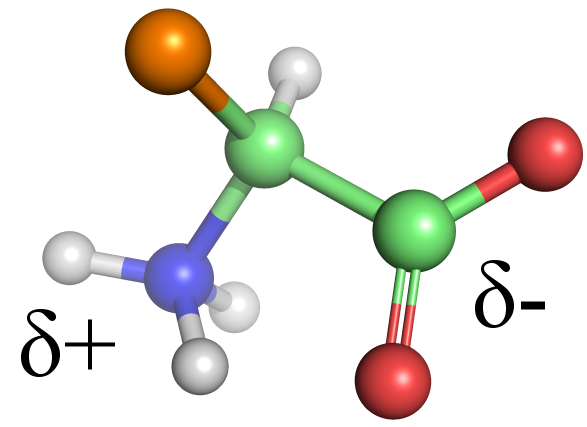
\includegraphics[width=0.40\textwidth]{./01-ProteinStructure/aminoacid/aminoacid.png}
\caption[An amino acid]{An amino acid. The R-group, which is variable between different amino acid types, is shown as a unified orange sphere. The net partial charges of the zwitterion
are shown in black text.}
\label{fig:intro:aminoa}
\end{center}
\end{figure}

The primary structure in turn dictates the formation of more complex secondary
and super-secondary structures. The core of globular proteins, which is compact and hydrophobic in nature, can be conceptually divided into  secondary structure elements which are stabilised by regular hydrogen bonding networks. Connecting these secondary elements are so-called ``random coil'' regions, also know as loops, which are intrinsically less regular
and more hydrophilic in nature.

Tertiary structure describes the association of these secondary elements. Longer single-polypeptide chains commonly form distinct globular
units termed domains, usually of around 100 amino acids in length. Domains are conserved throughout evolution both in terms of sequence and structure. It is their replication, mutation and recombination that
is thought to play a key role in driving the evolutionary process\cite{NATIVE:SUPERFAMILY:2007}. 

Finally, although not applicable to all proteins, quaternary structure describes the inter-relation of multiple polypeptide chains
 in the formation of protein complexes. These complexes can range in size from protein dimers totalling less than 150 amino acids to huge macromolecular complexes totalling many thousands of amino acids.



\subsection{The Native State} 

It is experimentally observed that denatured globular
proteins spontaneously refold into their native state once physiological
conditions are restored. This observation has the implication that the primary sequence of a polypeptide chain alone ultimately dictates its tertiary structure. The native fold represents an energetically stable structure on the hugely rugged folding landscape, postulated by the thermodynamic hypothesis to be the state with the lowest free energy\cite{NATIVE:Anfinsen1973}. The ability to predict this structural state from the polypeptide sequence alone is a central problem in molecular biology today, and is termed the
protein-folding problem. 

Despite a wealth of research, the problem of how the
chain folds into a single native conformation in the face of seemingly infinite conformational possibilities, is still poorly understood. The Levinthal paradox\cite{NATIVE:Levinthal1968} theorises that kinetic pathways for protein folding must exist, as it is estimated that a purely random conformational search of a \mer{100} polypeptide would take $10^{29}$ years\cite{NATIVE:Dobson1998}. 

By contrast, it is clear that the vast majority of naturally occurring proteins do spontaneously fold reliably and quickly into their native state, despite the astronomical number of possible conformations. They must, therefore, satisfy both a kinetic requirement for folding on an appropriate timescale and a thermodynamic requirement for a single stable folded conformation. The Levinthal paradox
is potentially
resolved by the concept that folding is guided by the rapid formation of local interactions, which then determine the further folding of the peptide. This suggests that local stretches of polypeptide form stable interactions and serve as nucleation points in the folding process.
 

Attempts to tackle the protein folding problem lie at the crossroads between the many avenues of science including biology, chemistry, physics, mathematics, statistics and computer science. Inroads towards greater understanding of native protein structure will result in more successful prediction of the native state
which will ultimately have many far reaching benefits.










\section{Protein Anatomy}

If the native state is to be predicted, it is critical that one has a clear picture of
the structural motifs that are found in globular proteins. This section illustrates common structural classifications and defines their major
features. 
\subsection{The Protein Backbone}
\label{section:intro:prot_backbone}

The polypeptide backbone can be well described in torsional space using just two backbone angles per residue, phi ($\Phi$) and psi ($\Psi$) (figure \ref{fig:intro:bb_torsion}).
The peptide group is a planar unit with a delocalised electronic structure and therefore inherently inflexible, owing to its partially double-bonded character. This  causes the Omega (\Omg) angle of the peptide group to usually lie very close to 180\degree\ corresponding to its trans-isomer, only very occasionally occupying 0\degree\ corresponding to the more sterically strained cis conformation (figure \ref{fig:intro:cis_trans}). 

\begin{figure}[hptb]
\begin{minipage}[b]{0.47\linewidth}
\centering
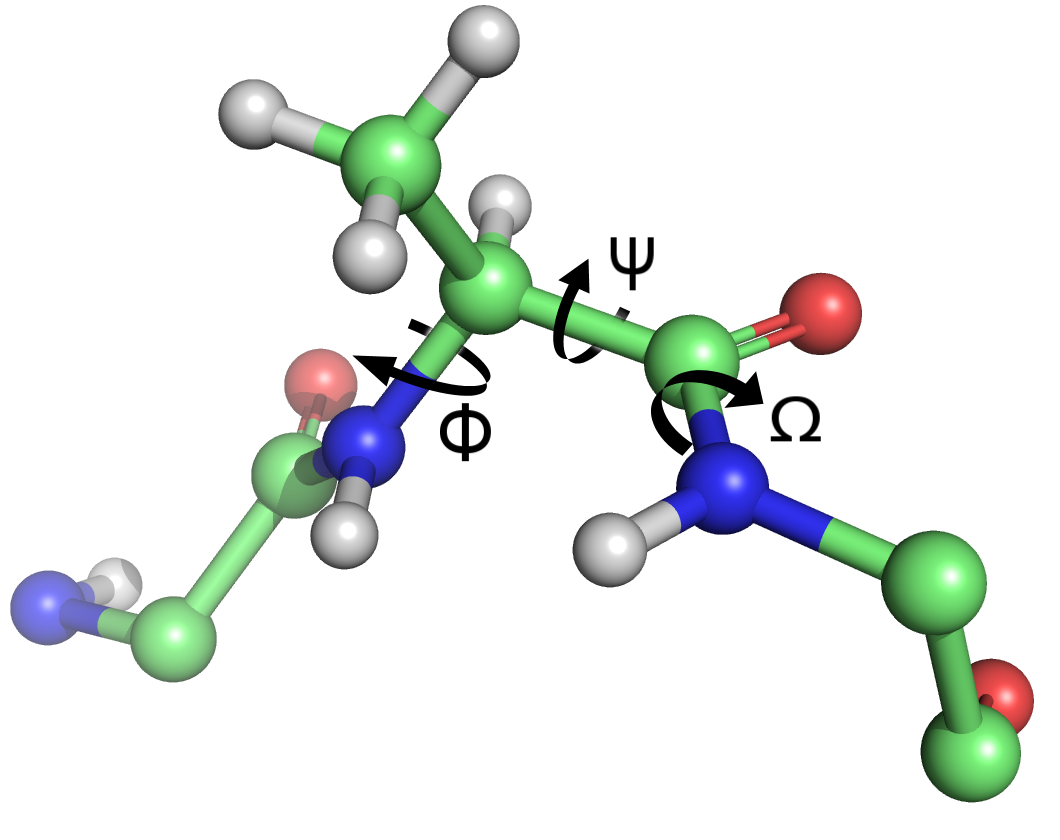
\includegraphics[width=1.0\textwidth]{01-ProteinStructure/structure/bb_torsion.png}
\caption{Protein backbone torsions.}
\label{fig:intro:bb_torsion}
\end{minipage}
\hspace{0.5cm} % To get a little bit of space between the figures
\begin{minipage}[b]{0.47\linewidth}
\centering
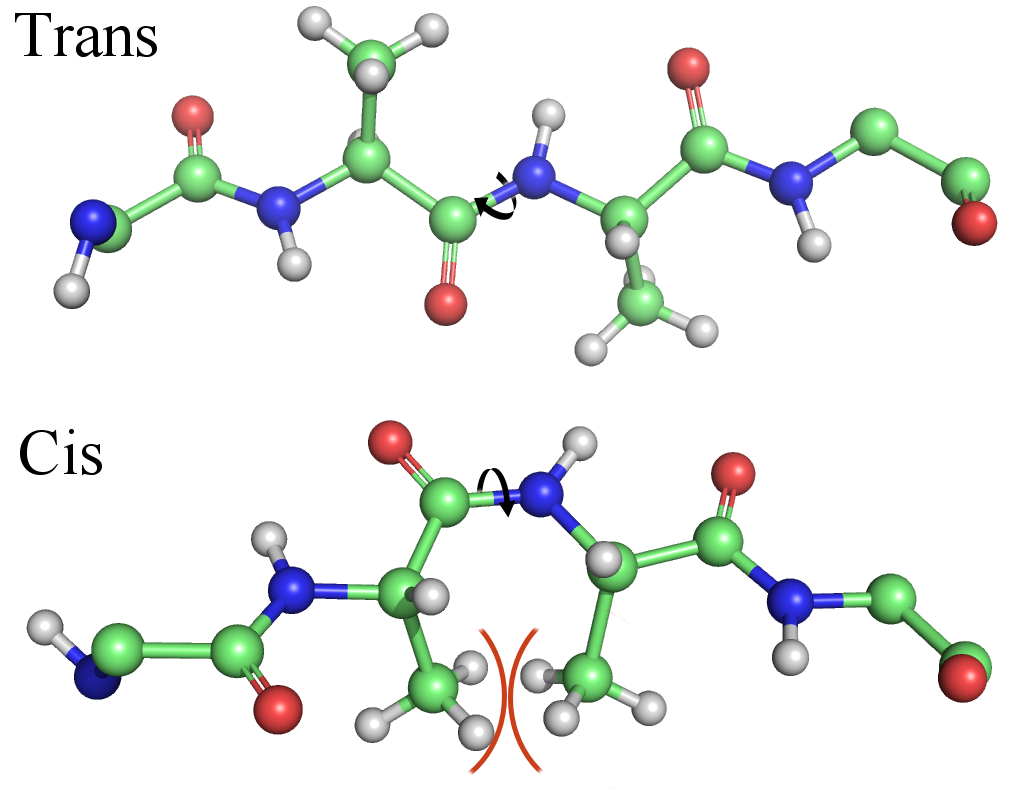
\includegraphics[width=1.0\textwidth]{01-ProteinStructure/structure/cis_trans.png}
\caption{The cis and trans-peptide group conformations.}
\label{fig:intro:cis_trans}
\end{minipage}
\end{figure}

\subsection{Amino Acid  \Sidechains}

Each of the 20 naturally occurring amino acids is defined by its  \sidechain. The major classes of these include   small, hydrophobic, nucleophilic, amide,
acidic, basic and aromatic residues. Figure \ref{fig:intro:chi} shows the bonds that are available for rotation, which are commonly annotated with the letter $\chi$ and numbered
away from the central \mainchain\ \ca-atom. The exact number of possible $\chi$-angles is obviously dependent on the residue. 


\begin{figure}[hptb]
\begin{center}
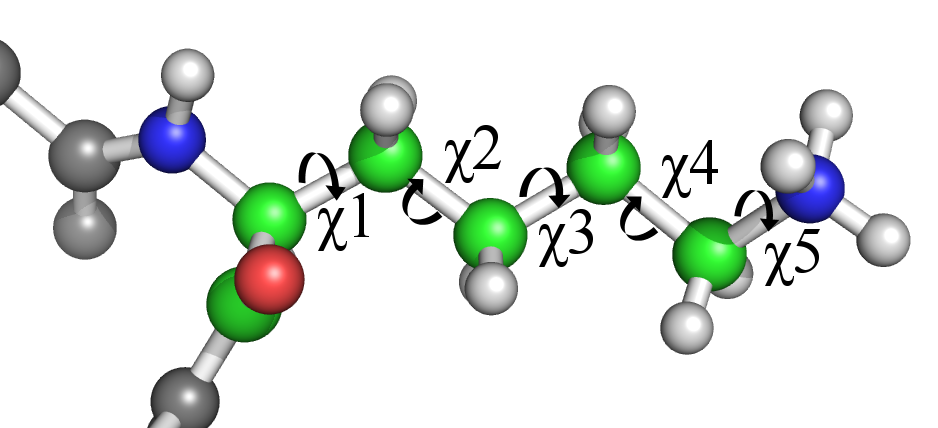
\includegraphics[width=0.6\textwidth]{01-ProteinStructure/sidechain/chi.png}
\caption{The \sidechain\ $\chi$ torsions of lysine.}
\label{fig:intro:chi}
\end{center}
\end{figure}

\Sidechain\ $\chi$-angles can be used to describe the rotational states  of the \sidechain. Following clustering of the the \sidechain\ conformations within the PDB, distinct conformational classes can be defined. Libraries of these commonly populated states, termed rotamer libraries\cite{NATIVE:Kan93,NATIVE:Dun97,NATIVE:Shetty2003}, are available for use in protein modelling.


\subsection{The Ramachandran Plot}
\label{section:intro:ramachandran}

Residue backbone conformations are generally visualised by the using a Ramachandran plot\cite{NATIVE:Ramachandran1963,NATIVE:Ramachandran1968} (Figure \ref{fig:intro:ramachandran}), which plots the values of the \phipsi\ backbone torsional angles against each other and in which regions of high population density can clearly be seen. 

\begin{figure}[hptb]
\begin{minipage}[b]{0.47\linewidth}
\centering
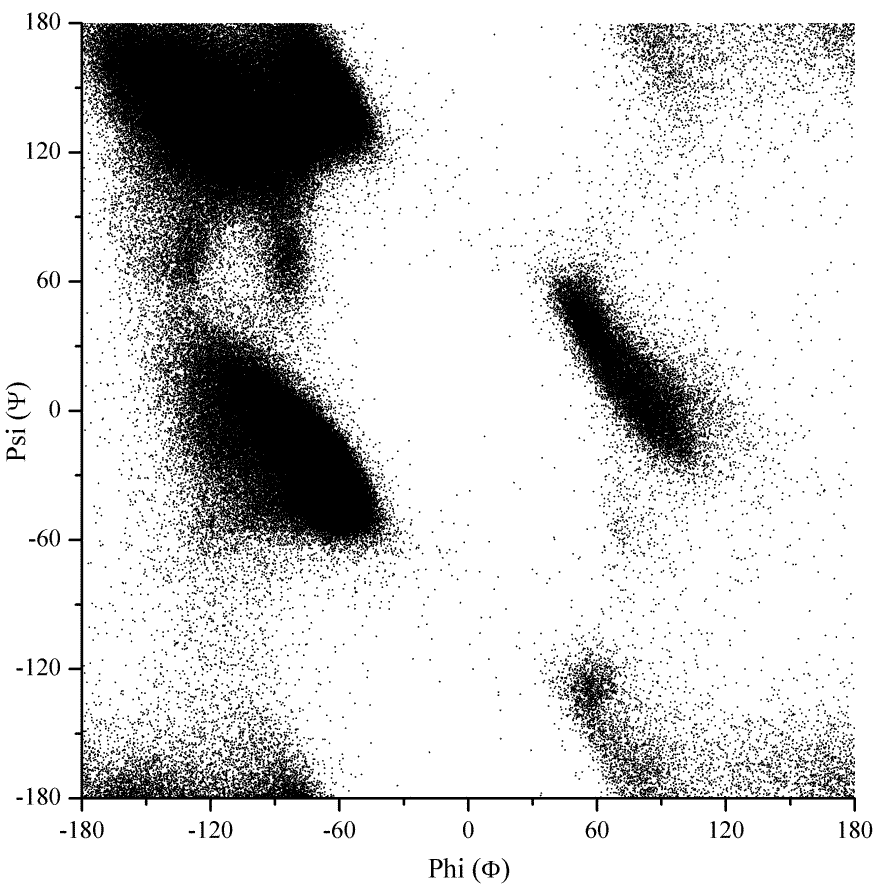
\includegraphics[width=1.0\textwidth]{./01-ProteinStructure/ramachandran/ram_scatter.png}
\end{minipage}
\hspace{0.5cm}
\begin{minipage}[b]{0.47\linewidth}
\centering
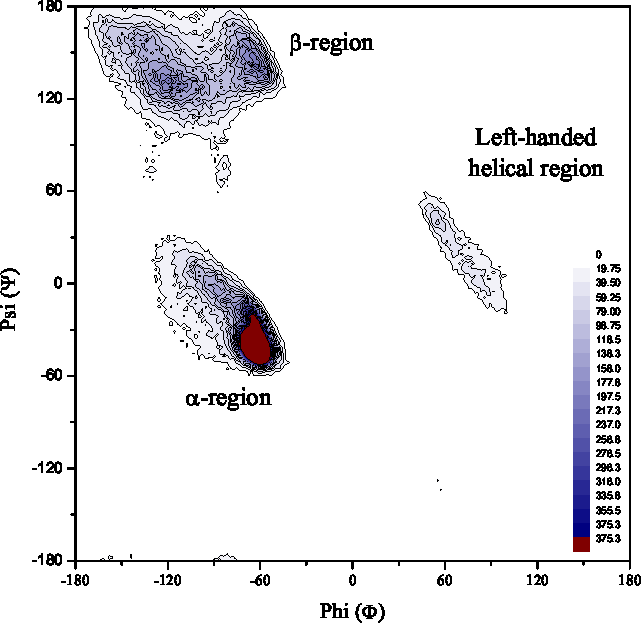
\includegraphics[width=1.0\textwidth]{./01-ProteinStructure/ramachandran/ram_Contour.pdf}
\end{minipage}
\caption[The typical Ramachandran plot]{The typical Ramachandran plot. Plotted using \xray\ crystallographic data from all non-proline and non-glycine residues from structures of \textgreater 1.8\AA\ resolution within the PDB. Left: A scatter plot. Right: A contour plot illustrating the density of data;  annotated with the class of secondary structure that each populated region represents. }
\label{fig:intro:ramachandran}
\end{figure}

A measure of structural quality can be obtained by looking at deviations from these ``ideal'' Ramachandran distributions for a given structural model, however at least mild deviations do occur in all high quality PDB structures. An individual amino acid may tolerate small local deviations from its idealised backbone torsion angles in order to optimise stabilising tertiary interactions in the protein as a whole, such as hydrogen bonding, hydrophobic burial or substrate and ligand interactions in an active site. These deviations can be clearly seen in the ``haze'' of data points around the high density idealised regions.






\subsection{Secondary Structures}

Inspection of the Ramachandran plot in figure \ref{fig:intro:ramachandran} clearly reveals three regions of extremely high propensity. These highly populated
regions represent the basic regularised secondary structural motifs of the
\ahelix, \bstrand\ and left-handed helix. The vast majority of the structure within the core of globular proteins  is described by these motifs. 


\al-helices\cite{NATIVE:Pauling1951:Helix} and \be-strands\cite{NATIVE:Pauling1951:Sheet}, shown diagrammatically in figure \ref{fig:intro:secstruc}, were originally predicted by Pauling and Corey, as early as 1951, on the grounds of geometry and hydrogen bonding alone.
The right-handed \ahelix\ is the most common form of helix in protein structure,
exhibiting 3.6 residues per turn. Critically it is the specific repeating
hydrogen bonding pattern which defines an \ahelix. Hydrogen bonds
within helices are local-sequence interactions whereby the N--H group of each participating amino acid forms a bond with the C=O group of the amino acid four residues earlier.
\bstrands\  are not  common in isolation, but instead form sheets stabilised by regular hydrogen bonding patterns. As opposed to the local bonding
interactions of helices, \bstrands\ require long-range interactions within
the polypeptide chain. \bsheets\ come in two varieties; the parallel and anti-parallel.

\begin{figure}[p]
\begin{center}
\subfigure[A typical \ahelix]{%
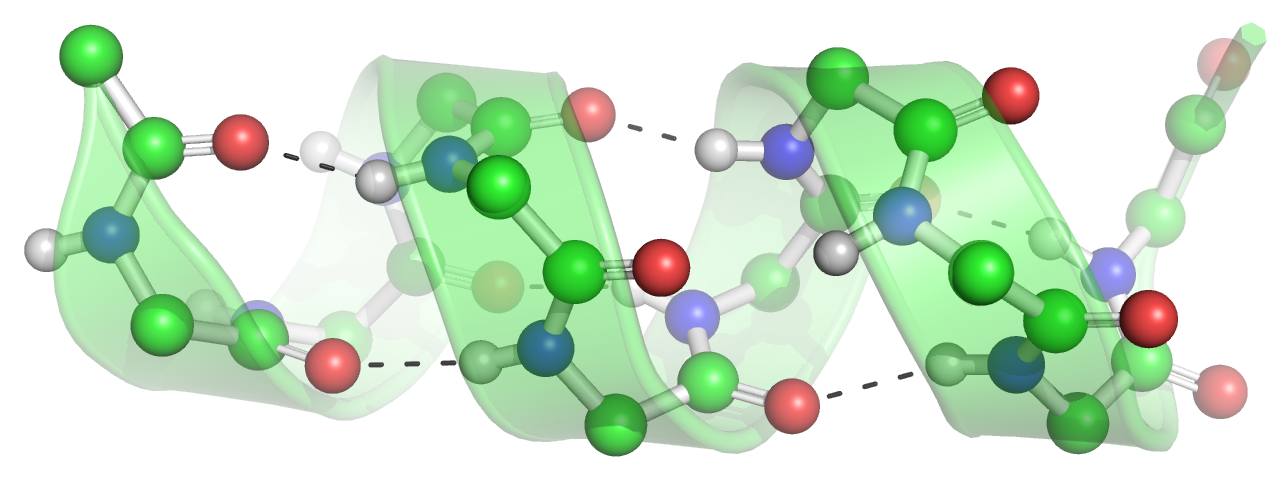
\includegraphics[width=0.8\textwidth]{./01-ProteinStructure/secstruc/helix.png}%
}
\quad
\subfigure[A typical anti-parallel \bsheet]{%
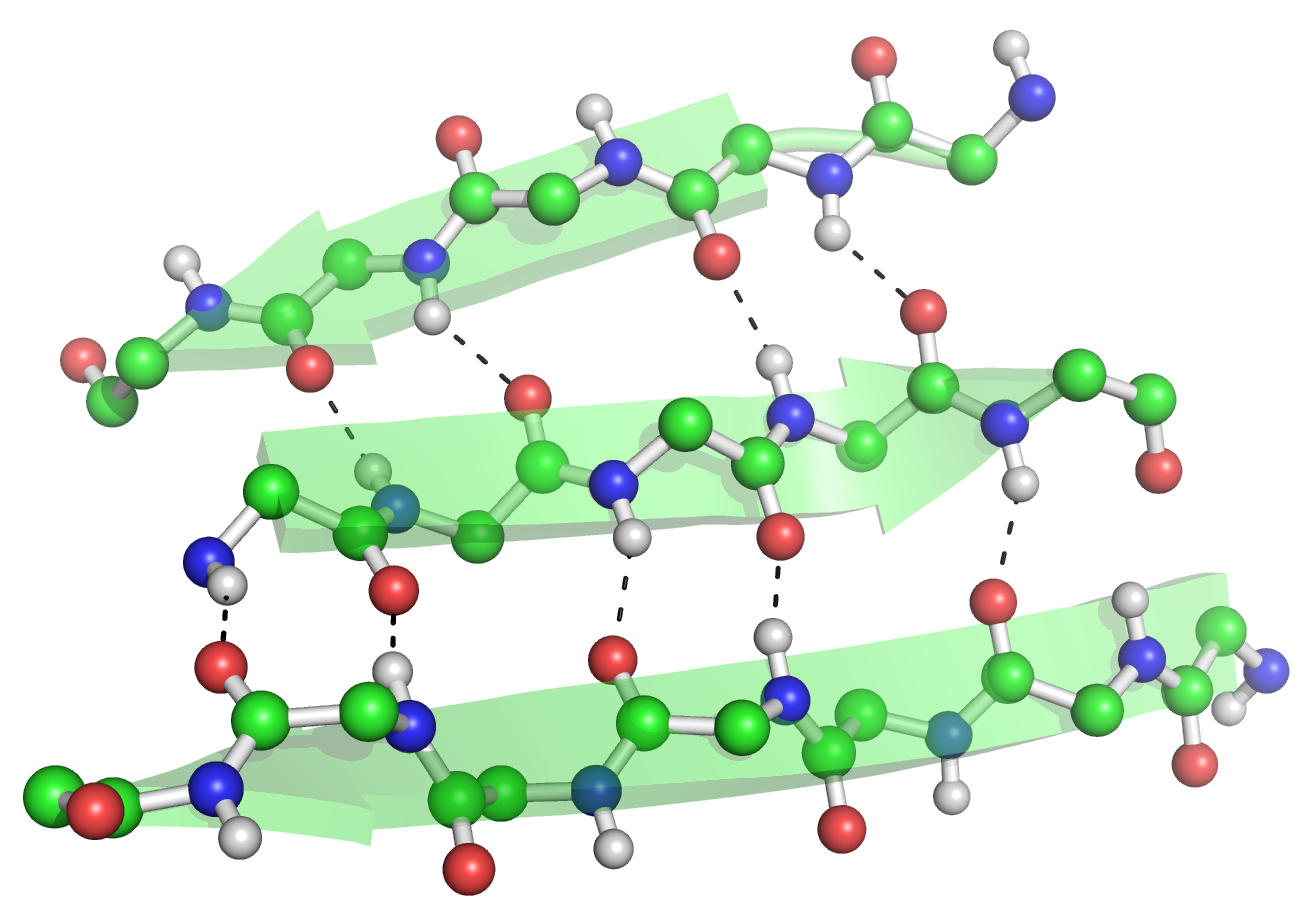
\includegraphics[width=0.8\textwidth]{./01-ProteinStructure/secstruc/antiparallel_strand.png}%
}
\quad
\subfigure[A typical parallel \bsheet]{%
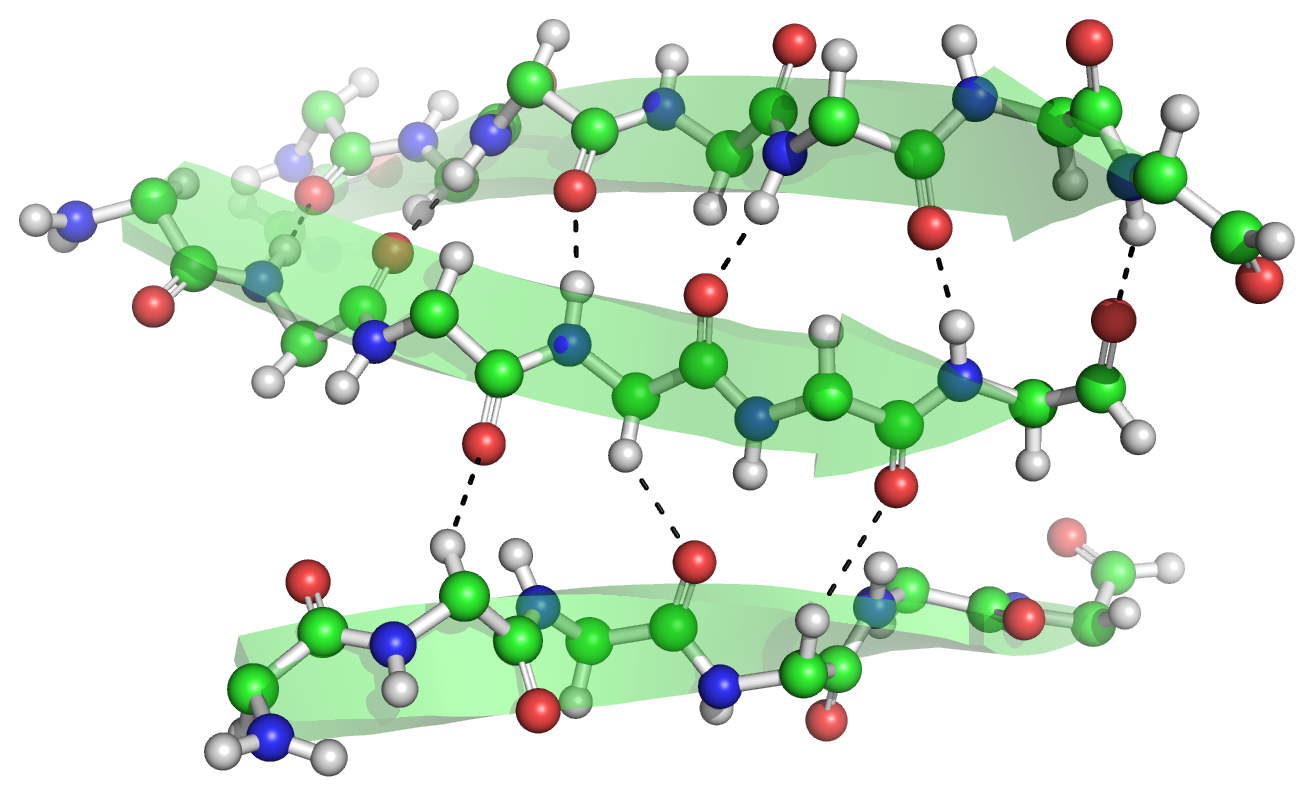
\includegraphics[width=0.8\textwidth]{./01-ProteinStructure/secstruc/parallel_strand.png}%
}
\caption[Basic secondary structure in globular proteins]{Basic secondary structure in globular proteins. Hydrogen bonds are shown as black dashed
lines. Images created using \pymolV.}
\label{fig:intro:secstruc}
\end{center}
\end{figure}

In addition to very common \al-helical and \bsheet\ structures in globular proteins, there are also other less common forms of secondary structure, as described in table \ref{table:intro:secstruc}. These include alternative helical forms
which are defined by repeating units containing different numbers of amino acids\footnote{For helical structural definitions, hydrogen bonding is defined in terms of $i$. $i \rightarrow i+x$ signifies that within a given repeat unit, the first residue forms a hydrogen bond with the residue $x$ further ahead in the primary sequence. This does not apply to \bstrands\ as their hydrogen bonding occurs between long-range
sections of the primary sequence.}. It is worth mentioning that these helices are less stable than the
\ahelix\ and are therefore typically much shorter. In all regular secondary structures, it is the  repeating pattern of hydrogen bonding that gives the
structure its stability.

\begin{table}[htbp]
\begin{center}
\begin{tabularx}{0.99\textwidth}{+l^r^r^c^X}
\toprule
\rowstyle{\bfseries}
  Name &   $\Phi$  &   $\Psi$  & Handed &  Comments \\
\midrule
  3\subscript{10}-helix   & -49 & -26 & right & Hydrogen bonded $i \rightarrow i+3$     \\
  \ahelix\                & -60 & -45 & right & Hydrogen bonded $i \rightarrow i+4$     \\
  $\pi$-helix             & -57 & -80 & right & Hydrogen bonded $i \rightarrow i+5$     \\
  Left-handed helix       &  57 &  47 &  left &                                         \\
  Type-II helices         & -79 & 150 &  left & Formed by poly-glycine and poly-proline \\
  Collagen helix          & -51 & 153 &  left & Formed by three left-handed helices     \\
\midrule
  \bstrand                &-119 & 113 &   --  & Parallel \bsheet                        \\
  \bstrand                &-139 & 135 &   --  & Anti-parallel \bsheet                   \\
\bottomrule
\end{tabularx}
\caption{The names, averaged \phipsi\ values and comments associated with the common regularised structure classifications.}
\label{table:intro:secstruc}
\end{center}
\end{table}









\subsection{Distortions in Secondary Structure }

When Pauling and Corey produced the original definitions for \ahelixs\ and \bsheets\, they were based purely upon strict geometric criteria and so made no comment
on the potential distortion of such structures. By contrast, in real proteins within the PDB
all manner of distortions in these structures can be found.  In light of
this, many examples exist where it is unclear as to whether a region should
be annotated as a regular structure, a secondary structure break or part of a surface loop structure. Within these ambiguous regions some distinct structural
motifs can be defined, which are termed secondary structure distortions.

 
\subsubsection{Helical Distortions}

Helices in real protein structures exhibit averaged \phipsi\ angles that differ slightly from those present for a textbook ideal helix. 
Of 48 analysed \ahelixs\, only 15\% are considered to be truly linear, of the remainder 17\% are kinked and 58\% are curved\cite{AUTO:HelixKinks}.

Helix curvature is generally caused by differences in hydrogen bonding geometry
on the two sides of the helix caused by carbonyl-solvent and \sidechain\ interactions on the solvent exposed helical face. This  curvature is often centred on the hydrophobic side of the helix. Overall, curvature is not expected to be energetically expensive and has been estimated at 
$<2$ \kcalmol\ for a five turn helix.

Kinks are often caused by proline residues, which are  conserved
 between homologous protein sequences, signifying their structural/functional importance. The angle of such kinks is usually of the order of 26\degree.
It is not the proline residue itself that causes the kink, as the \phipsi\
angle of proline is helical, but the  proline \sidechain\ which imposes
non-helical backbone torsions on the preceding residue. For this reason,
proline is commonly found at the start of \ahelixs.


\subsubsection{Beta-bulges} 

The $\beta$-bulge\cite{STRUCTURE:Mil87,STRUCTURE:Mil88:Bulge,STRUCTURE:Chan1993} is a small piece of non-repetitive structure that can occur by itself in loop regions, but which most often occurs as a common irregularity in anti-parallel $\beta$-structure. Almost all bulges occur at the edge of a sheet, with the
bulged strand being the outermost one. Most examples involve anti-parallel strands, with fewer than 10\% of $\beta$-bulges being between parallel strands
even though the ratio of anti-parallel to parallel $\beta$-sheets
is approximately 4.5 to 1\cite{STRUCTURE:Chan1993}. $\beta$-bulges usually occur due to the introduction of an additional residue with helical \phipsi\ angles into a \bsheet\ which causes a $\sim$10\degree\ twist. 
The two most common kinds are the Classic and G\subscript{1} bulges with other less common types, namely wide, bent and special. All $\beta$-bulge types have additional sub-types dependent on the
exact structural features.

\begin{figure}[hptb]
\begin{center}
\subfigure[A classic $\beta$-bulge from 1GL0 showing the accepted annotation of residues 1, 2 and X -- residues Phe41, Cys42 and Lys33 respectively.]{
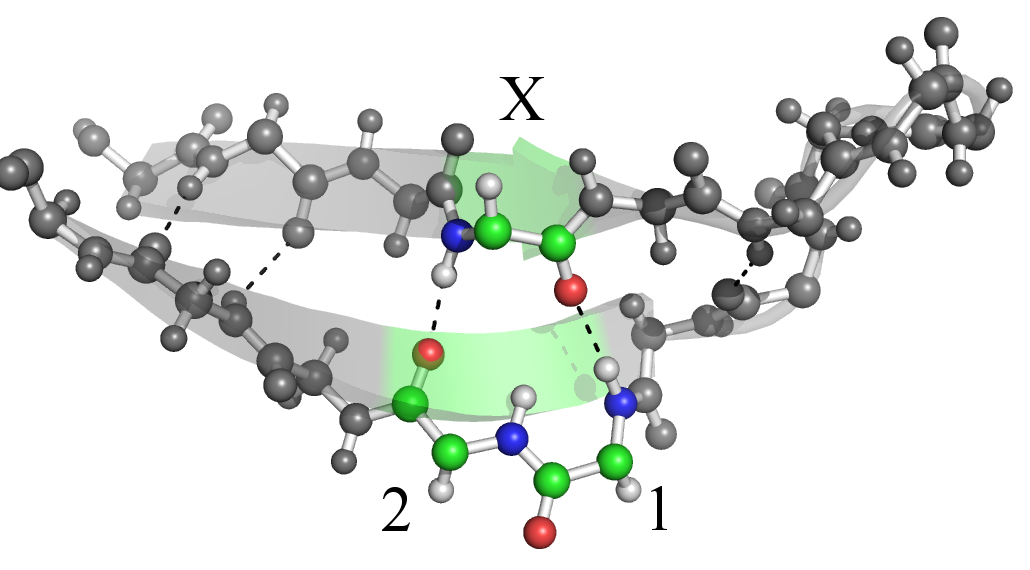
\includegraphics[width=0.8\textwidth]{01-ProteinStructure/bulges/bulge.png}
}

\subfigure[A wide $\beta$-bulge from 2ER7 showing the accepted annotation of residues 1, 2 and X -- residues Thr205, Ser206 and Thr195 respectively.]
{
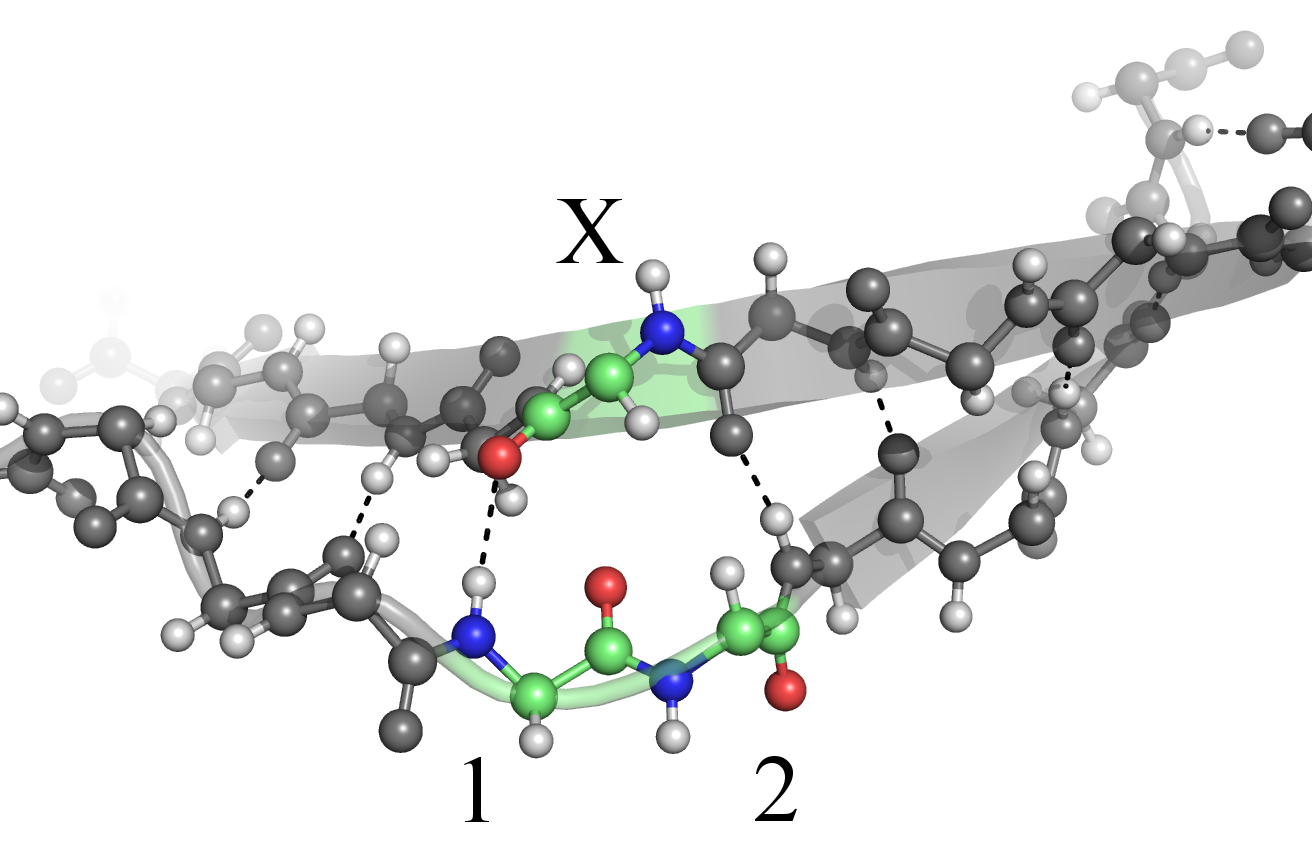
\includegraphics[width=0.8\textwidth]{01-ProteinStructure/bulges/bulge-wide.png}
}
\caption[Typical \be-bulges]{Typical \be-bulges. The classical and wide classifications
are shown. Hydrogen bonds are shown as dashed lines. Only the resides involved in the bulge itself are shown in colour.}
\label{fig:intro:bbulge}
\end{center}
\end{figure}

\begin{description} \isep

\item[Classic] $\beta$-bulges, illustrated in figure \ref{fig:intro:bbulge}-a, occur between the narrowly-spaced pair of hydrogen
bonds on anti-parallel strands. A single residue is inserted, causing the bulge. The \sidechains\ of positions 1, 2, and $X$ are all on the same side of the \bsheet. Residue 1 is in approximately $\alpha$-helical conformation and residues 2 and $X$ in approximately normal $\beta$ conformation.

\item[Wide] $\beta$-bulges, by contrast, occur between the widely-spaced pair of hydrogen bonds on anti-parallel strands. A typical example is shown
in figure \ref{fig:intro:bbulge}-b. They are apparently much less constrained than the narrow classic bulges, since they occur with a great variety of backbone conformations; they are however less common. 

\item[Special] $\beta$-bulges are the most unusual and include a G\subscript{x} sub-type, so named because they have a high propensity for glycine in position $X$.
Special bulges are defined to have between two and
four extra residues on one strand.
\item[G1] $\beta$-bulges are often observed to occur at the loop end of beta-hairpins. G1 $\beta$-bulges, defined by characteristic hydrogen bonding and dihedral angles, are sometimes found to act as a sort of turn in the absence of any adjacent anti-parallel $\beta$-hairpin.

\end{description}

$\beta$-bulges are not only of structural importance, but can also be functionally
relevant. For example, in superoxide dismutase, two bulges at the end of two functionally important loops causes them to curl away from the main $\beta$-barrel to enclose the active site\cite{STRUCTURE:Getzoff1989}. In specific cases like the Immunoglobulin-family proteins, $\beta$-bulges are conserved to aid in dimerisation of the Ig domains.
























\subsection{Loop Structure}
\label{section:loop_structure}

Mainly during the 1980s it was recognised that ``random-coil'' regions in
proteins are not, after all, completely random. Additional distinct structural motifs exist\cite{NATIVE:anatomy}, but are simply harder to categorise than regular secondary structure. It is convention to refer to shorter loops as ``simple~loops'', whereas longer loops which may contain one or more classified simple loop types are termed ``compound~loops''. 

Surface loops range in length from 1 to as many as 30 residues, although the majority are less than 12 residues in length\cite{METHOD:Fis2000}. Protein surface loops often play key functional roles and many residues are intimately involved in active sites. Some loops exhibit high structural diversity and flexibility, which may mean they are not structurally or functionally well defined\cite{METHOD:Heuser2004}.

This section describes the main classes that have been described in the literature. The knowledge of these structures should be exploited in order to make loop modelling more representative and efficient.





\subsubsection{Disallowed Regions of the Ramachandran Plot}

As has been discussed, the distribution on a Ramachandran plot shows clear bias
towards a small number of distinct \phipsi\ locations. There is however a significant
amount of data that does not occupy these regions, even in structures  which
have a high
degree of experimental confidence.
These regions  were originally referred to as
``disallowed'' in hard-sphere modelling studies performed on the protein
backbone\cite{NATIVE:Ramachandran1968}.  Recent studies however have analysed data
in these disallowed regions to see what structural motifs they relate to\cite{NATIVE:DISALLOWED,NATIVE:Gunasekaran1996}.
Other structural studies have focused on individual residues occupying specific disallowed regions\cite{NATIVE:Vega2000}. It is thought that excursions into the Ramachandran prohibited regions will usually incur a strain of at least 5 \kcalmol, in contrast to typical free energy changes for protein folding which are in the range of -5 to -15 \kcalmol\cite{NATIVE:Her91}.



In the most recent study, which focused exclusively on extremely high resolution
structures, it was found that out of a total of 63,949 non-glycine residues, only 241 (0.4\%) were found in the entirely disallowed region. Around a 70\% majority of residues located in disallowed regions are solvent-exposed, indicating
a vastly increased importance in loop structure\cite{NATIVE:DISALLOWED}. It is important to note that although a low proportion of residues exist in a disallowed region, around 3\%, 6\%
and 8\% short and medium and long length loops respectively do have at least one residue in a disallowed region (section \ref{section:loop_stats}). 

These large deviations from allowed Ramachandran regions, which cannot be ascribed to experimental error, are usually found exhibiting compensating interactions. The loss of hydrogen bonding is less important at the protein surface compared to the protein core due to solvation effects.
However, \sidechain\ or non-regular hydrogen bonds, are often be involved and many are described throughout the remainder of this section. 

Figure \ref{fig:intro:disallowed} shows clustered disallowed  regions. Clusters II and III normally correspond to residues which are stabilised by hydrogen bonds in turns. Residues in cluster I are sometimes stabilised by \sidechain\ hydrogen bonding and occur as part of distorted \bstrands. Cluster IV is found in some unusual conformations, one example of which involves a tyrosine residue \sidechain\ interaction.\ In this example, the aromatic face of the \sidechain\ was involved in a C--H $\to$ $\pi$-orbital interaction and a hydrogen bond was formed by the terminal oxygen\cite{NATIVE:Sam2000}. Cluster V can be considered to be an extension of the beta region -- a nomenclature artefact produced by the original definition of the \be-region in the original disallowed region study\cite{NATIVE:Gunasekaran1996}.
 
\begin{figure}[hptb]
\vspace{0.4cm}
\begin{minipage}[b]{0.47\linewidth} % 0.5 for half the page
\centering
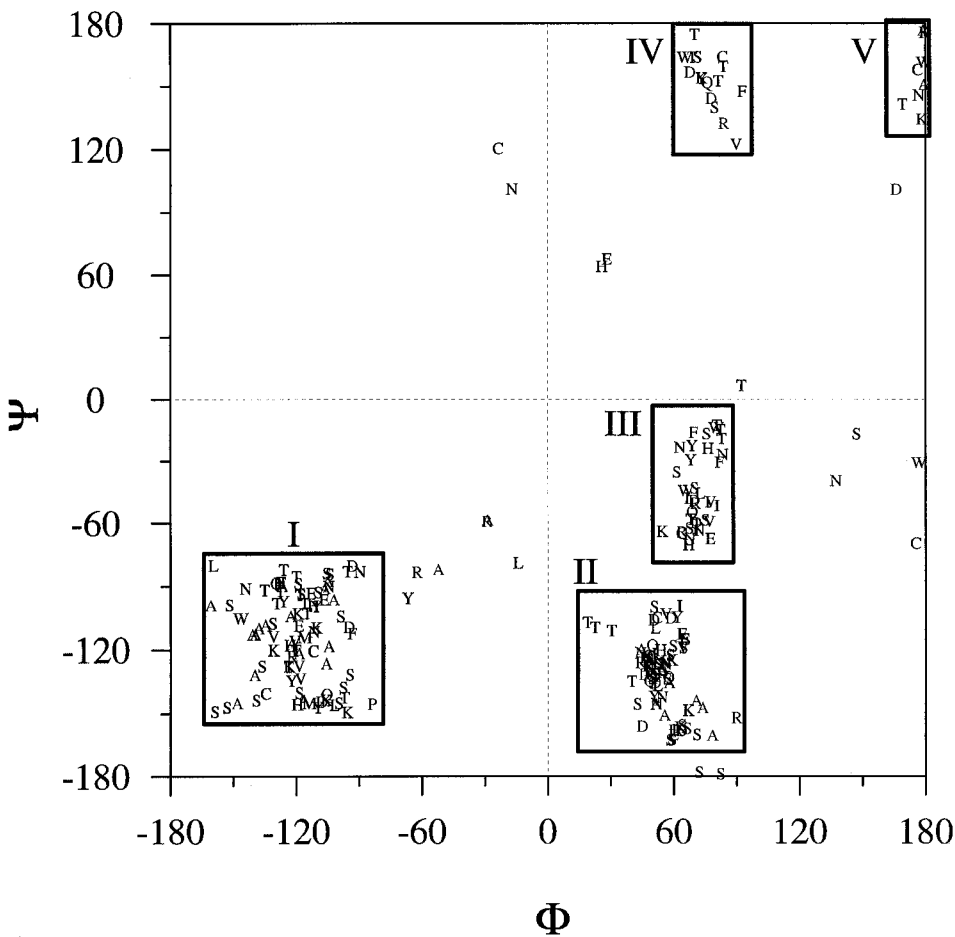
\includegraphics[width=1.0\textwidth]{01-ProteinStructure/ramachandran/disallowed.png} % 1.0 to take ALL the half page
\end{minipage} 
\hspace{0.4cm} % To get a little bit of space between the figures
\begin{minipage}[b]{0.47\linewidth} % 0.5 for half the page
\centering
\begin{small}
\begin{tabularx}{1.0\textwidth}{+c^X}
\toprule
\rowstyle{\bfseries} Cluster & Residue Preference \\
\midrule
 I & Ser, Pro (low incidence) \\
 II & Ser, Asp, Asn, Polar and Leu \\
 III & Ser, Aromatic, not Ala, Ile (low incidence)  \\
 IV & Ser, Aromatic, not Ala  \\
\bottomrule
\end{tabularx}
\end{small}
\caption[Disallowed regions of the Ramachandran map.]{Disallowed regions of the Ramachandran map in 363 high resolution chains. (Figure adapted from\cite{NATIVE:DISALLOWED}.)}
\label{fig:intro:disallowed}
\end{minipage}
\end{figure}

Conformational analysis reveals that for these disallowed regions and also cis-containing peptides\cite{NATIVE:Her91} there are actually relatively few sterically strained features present. Those steric infringements that do occur are located overwhelmingly in regions concerned with function, which is most likely due to the greater precision necessary for ligand binding and catalysis, compared with the requirements of satisfactory folding. 








\subsubsection{Tight-Turns}
\label{section:intro:tightturns}

Tight-turns are abundant in globular proteins and were recently reviewed\cite{STRUCTURE:Cho2000}. A tight-turn in protein structure is defined as a site of no more than six residues where the polypeptide chain reverses and folds back on itself by around 180\degree. The peptide concerned must not be in a helical conformation. A turn formed by seven or more amino acids is not considered as a tight-turn, but rather as a ``loose turn''. The classes of tight-turns are categorised by loop length -- $\delta$-turn\cite{STRUCTURE:Ton80}, $\gamma$-turn\cite{STRUCTURE:Nem72,STRUCTURE:Mil88}, $\beta$-turn\cite{STRUCTURE:Mil86,STRUCTURE:Mil87,STRUCTURE:Hut94}, $\alpha$-turn\cite{STRUCTURE:Ton80,STRUCTURE:Pav96}, and $\pi$-turn\cite{STRUCTURE:Raj96,STRUCTURE:Kim76} -- which are formed by two, three, four, five, and six amino acid residues respectively. 

Tight-turns usually exhibit the following
features: 
\begin{enumerate} \isep
\item A distance between the \ca\ atoms of the first and last residue of $<$7\AA.\
\item In most cases an intra-turn hydrogen bond between the backbone oxygen of the first residue and backbone nitrogen of the last residue is present.
\item Multiple populated trajectories to reverse the chain direction as reflected by distinct preferred residue types at each position and characteristic backbone dihedral angles of the inner residues.
\end{enumerate}

\paragraph{$\delta$-turns} \isep
Of the tight-turn classes, the smallest is a $\delta$-turn involving only two amino acid residues. It is categorised by 1$\rightarrow$2 type, 2$\rightarrow$3 type, or C\subscript{8} form. The intra-turn hydrogen bond for a $\delta$-turn is formed between the backbone atoms NH\subscript{(i)} and CO\subscript{(i+1)}. 

\paragraph{$\gamma$-turns} \isep
$\gamma$-turns involve three residues and a hydrogen bond between the backbone atoms CO\subscript{(i)} and NH\subscript{(i+2)}. Residues in the $i$+1 position of a $\gamma$-turn are partly responsible for disallowed cluster 3 -- the $\Phi$=80\degree\, $\Psi$=-70\degree\ region of the Ramachandran plot \mbox{(figure \ref{fig:intro:disallowed})}. The typical averaged \phipsi\ values for this residue position have been analysed and the two main classes named (table \ref{table:intro:gammaturn}).

\begin{table}[hptb]
\begin{small}
\begin{center}
\begin{tabular}{+l^r^r}
\toprule
\rowstyle{\bfseries}
  Type &  $\mathbf{\Phi^{\circ}_{\mathbf{(i+1)}}}$ &   $\mathbf{\Psi^{\circ}_{\mathbf{(i+1)}}}$ \\
\midrule
  Classic $\gamma$-turn           & \color{red}{75} & \color{red}{-64} \\
  Inverse $\gamma$-turn           & -79 &  69 \\
\bottomrule
\end{tabular}
\caption[Possible $\gamma$-turn \phipsi\ angles]%
{Possible $\gamma$-turn \phipsi\ angles.
Residues occupying disallowed Ramachandran space are listed in red.
(Data \cite{STRUCTURE:Nem72}.)}
\label{table:intro:gammaturn}
\end{center}
\end{small}
\end{table}



\paragraph{$\beta$-turns} \isep
Perhaps the best-characterised and described class of turn is the $\beta$-turn. The $\beta$-turn has a long history of being re-categorised
with significant debate over the poorly represented classes.
Classification was originally defined based on \phipsi\ torsions in three distinct conformational classes and their \ca\ mirrors; types I, II, III and I', II', III' respectively\cite{STRUCTURE:Ven1968}.
As more structural information emerged the classes were expanded to ten types \cite{STRUCTURE:Lew73} and then reduced to just six types with a miscellaneous ``catch-all'' class to cover outliers\cite{NATIVE:anatomy}. In the most recent studies involving significantly more data, eight defined classes are used along with the miscellaneous class\cite{STRUCTURE:Hut94,STRUCTURE:Wilmot1990}.
Examples of these turn types are shown in figures \ref{fig:intro:bturn1} and \ref{fig:intro:bturn2} which are derived from the PDB structures in table \ref{table:intro:bturn_chains}. The \phipsi\ data is shown in Table \ref{table:intro:betaturn}.

\begin{figure}[p]

\begin{minipage}[b]{0.5\linewidth}
\centering
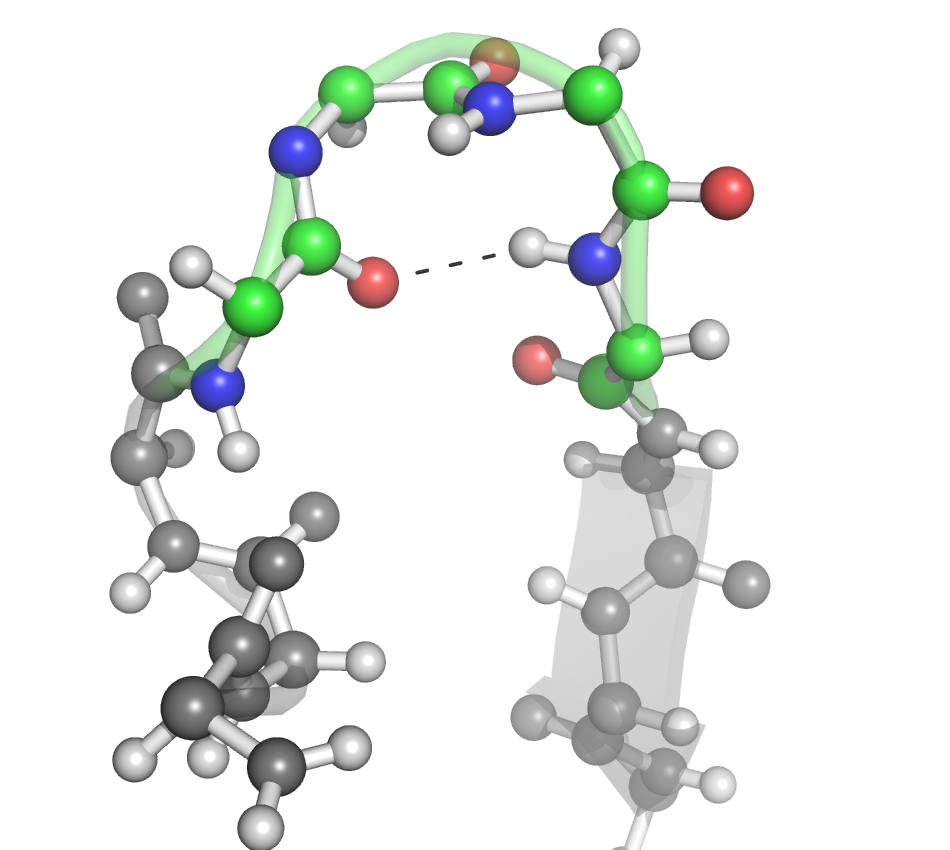
\includegraphics[width=1.0\textwidth]{./01-ProteinStructure/turns/beta-type-I.png}
\end{minipage}
\hspace{0.5cm}
\begin{minipage}[b]{0.3\linewidth}
\centering
Type I
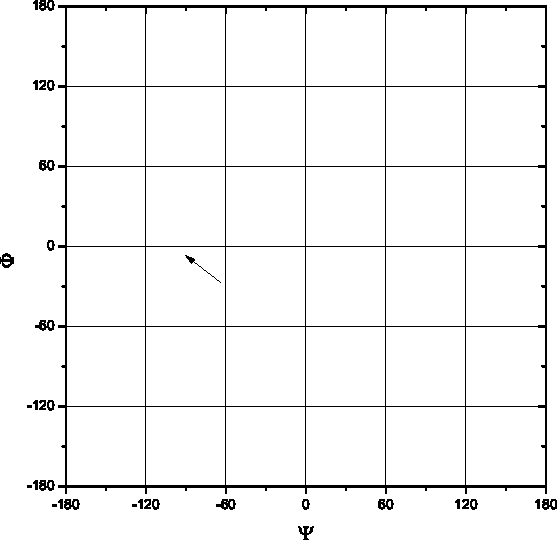
\includegraphics[width=1.0\textwidth]{./01-ProteinStructure/turns/beta-ram-type-I.pdf}
\end{minipage}

\begin{minipage}[b]{0.5\linewidth}
\centering
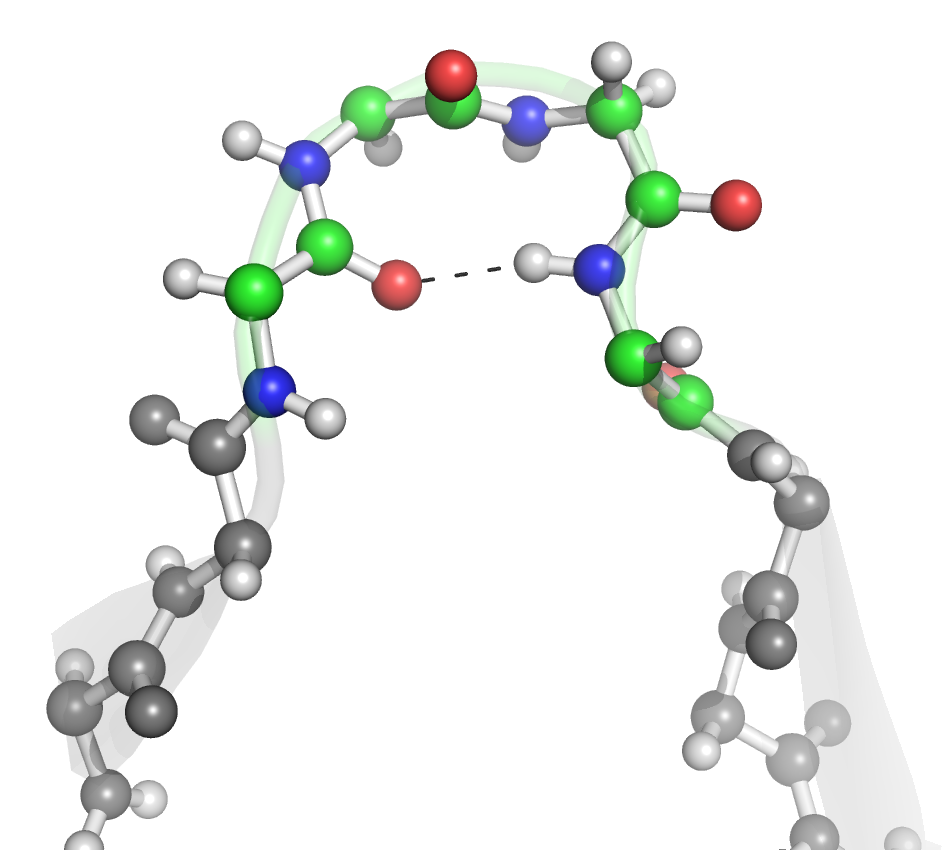
\includegraphics[width=1.0\textwidth]{./01-ProteinStructure/turns/beta-type-II.png}
\end{minipage}
\hspace{0.5cm}
\begin{minipage}[b]{0.3\linewidth}
\centering
Type II
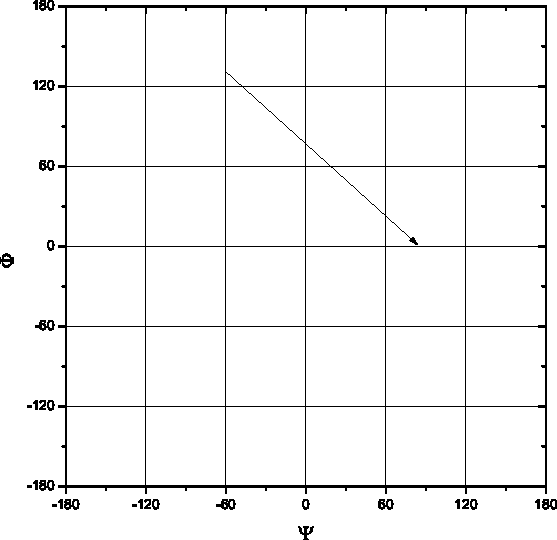
\includegraphics[width=1.0\textwidth]{./01-ProteinStructure/turns/beta-ram-type-II.pdf}
\end{minipage}

\begin{minipage}[b]{0.5\linewidth}
\centering
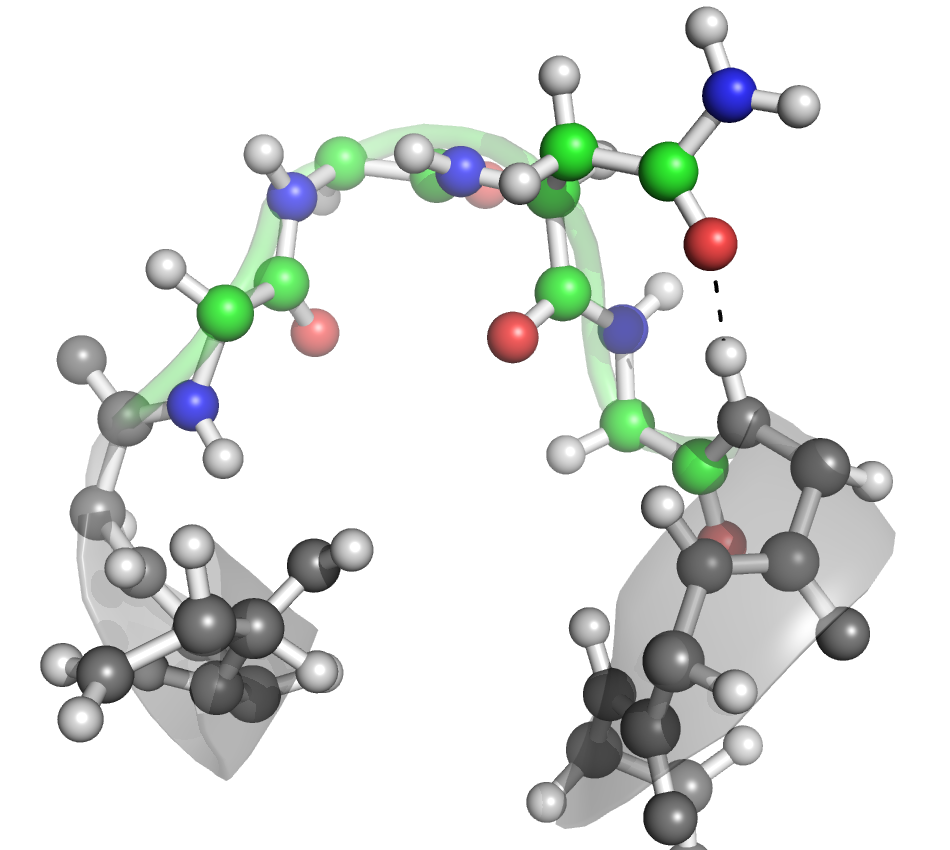
\includegraphics[width=1.0\textwidth]{./01-ProteinStructure/turns/beta-type-VIII.png}
\end{minipage}
\hspace{0.5cm}
\begin{minipage}[b]{0.3\linewidth}
\centering
Type VIII
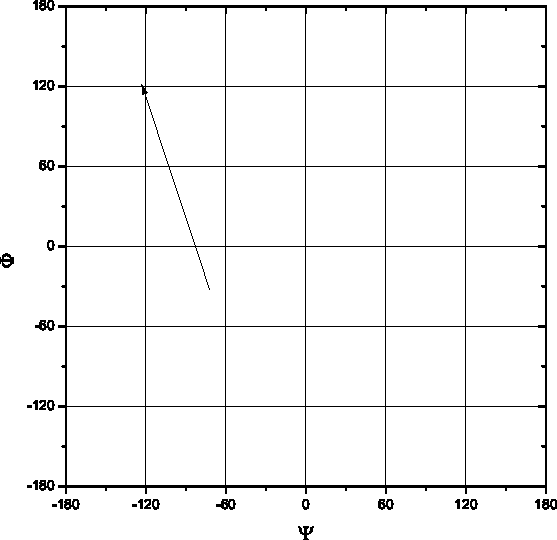
\includegraphics[width=1.0\textwidth]{./01-ProteinStructure/turns/beta-ram-type-VIII.pdf}
\end{minipage}

\caption[$\beta$-turns of class I, II and VIII]{$\beta$-turns of class I, II and VIII: Types I and II are the most common classical types. Non-classical
type VIII turns show no
intra-chain hydrogen bond, but are stabilised instead by a \sidechain$\rightarrow$backbone hydrogen bond. Ramachandran plots are presented showing residues $i$+1 and $i$+2.}
\label{fig:intro:bturn1}

\end{figure}

\begin{figure}[p]

\begin{minipage}[b]{0.5\linewidth}
\centering
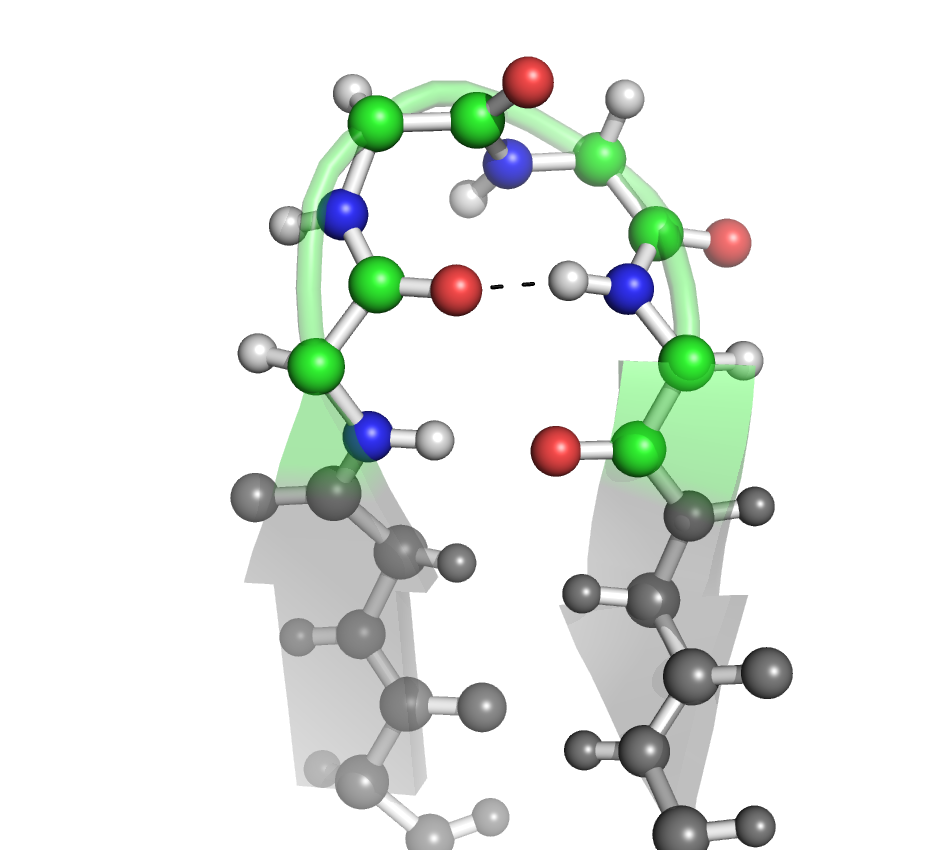
\includegraphics[width=1.0\textwidth]{./01-ProteinStructure/turns/beta-type-Ip.png}
\end{minipage}
\hspace{0.5cm}
\begin{minipage}[b]{0.3\linewidth}
\centering
Type I'
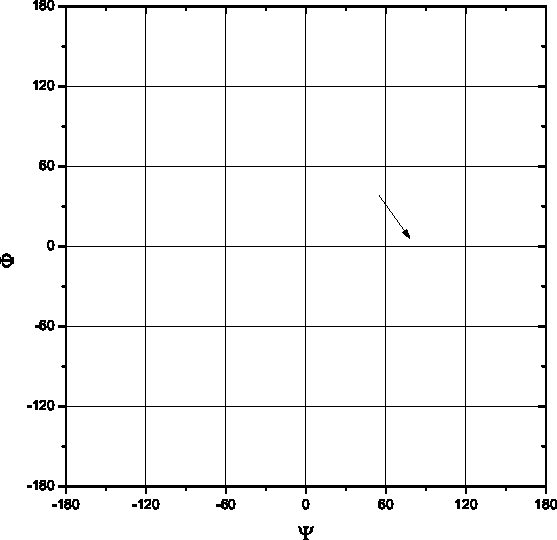
\includegraphics[width=1.0\textwidth]{./01-ProteinStructure/turns/beta-ram-type-Ip.pdf}
\end{minipage}

\begin{minipage}[b]{0.5\linewidth}
\centering
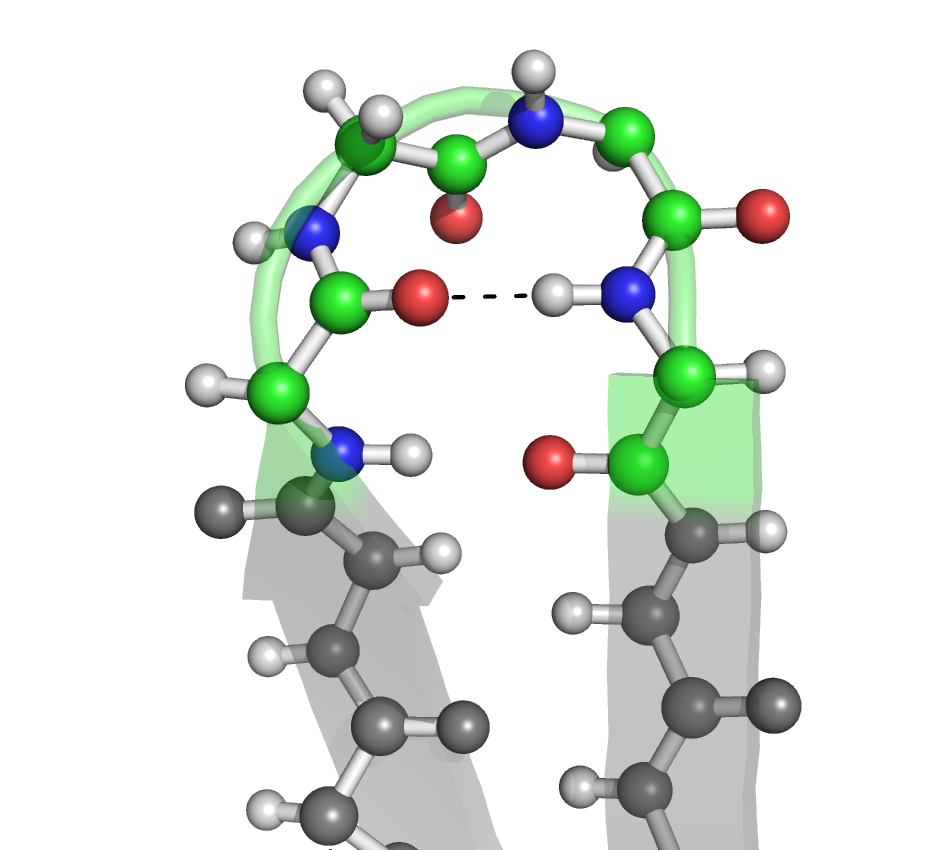
\includegraphics[width=1.0\textwidth]{./01-ProteinStructure/turns/beta-type-IIp.png}
\end{minipage}
\hspace{0.5cm}
\begin{minipage}[b]{0.3\linewidth}
\centering
Type II'
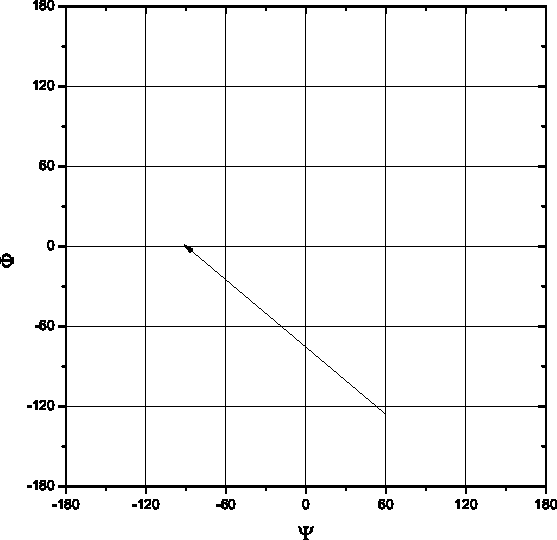
\includegraphics[width=1.0\textwidth]{./01-ProteinStructure/turns/beta-ram-type-IIp.pdf}
\end{minipage}

\caption[$\beta$-turns of class I' and II']{$\beta$-turns of class I' and II':
These are common classical turns involved in $\beta$-hairpins. Ramachandran plots are presented showing residues $i$+1 to $i$+2.}
\label{fig:intro:bturn2}

\end{figure}

\begin{table}[p]
\begin{small}
\begin{center}
\begin{tabular}{+c^c^c^c}
\toprule
\rowstyle{\bfseries}
  Type & PDBID & Residues & Sequence \\
\midrule
  I    & lCSE & 39-42   & HPDL \\
  II   & 1AAC & 38-41   & KVGD \\
  VIII & 1LZ1 & 86-90   & QDNI \\
  I'   & 1CGT & 293-296 & KDGA \\
  II'  & 1BBT & 19-22   & NGHT \\  
\bottomrule
\end{tabular}
\caption{PDB chains used in the $\beta$-turn figures \ref{fig:intro:bturn1} and \ref{fig:intro:bturn2}.}
\label{table:intro:bturn_chains}
\end{center}
\end{small}
\end{table}

\begin{table}[hbtp]
\begin{small}
\begin{center}
\begin{tabular}{+l^c^r^r^r^r^l}
\toprule
\rowstyle{\bfseries}
  $\beta$-turn & Plot\superscript{*}\ &
  $\mathbf{\Phi^{\circ}_{\mathbf{(i+1)}}}$ & $\mathbf{\Psi^{\circ}_{\mathbf{(i+1)}}}$
  &
  $\mathbf{\Phi^{\circ}_{\mathbf{(i+2)}}}$ & $\mathbf{\Psi^{\circ}_{\mathbf{(i+2)}}}$
  &
  Comment \\  
\midrule
I     & $\alpha_R\alpha_R$ &  -64  &  -27 &  -90 &  -7 & Most common type \\
II    & $\beta\gamma_L$    &  -60  &  131 &   84 &   1 & Common type \\
VIII  & $\alpha_R\beta$    &  -72  &  -33 & -123 & 121 & Common non-classic\\
I'    & $\alpha_L\gamma_L$ &   55  &   38 &   78 &   6 & Forms $\beta$-hairpins \\
II'   & $\epsilon\alpha_R$ & {\color{red}{60}}  & {\color{red}-126} &  -91 &   1 & Forms $\beta$-hairpins \\
VIal  & $\beta\alpha_R$    &  -64  &  142 &  -93 &   5 & --\\
VIa2  & $\beta\alpha_R$    & -132  &  139 &  -80 & -10 & --\\
VIb   & $\beta\beta$       & -135  &  131 &  -76 & 157 & --\\
IV    & --                  &  -61  &   10 &  -53 &  17 & Miscellaneous class\\
\bottomrule
\end{tabular}
\caption[$\beta$-turn classes and corresponding averaged \phipsi\ angles]{$\beta$-turn classes and corresponding averaged \phipsi\ angles.
Residues occupying disallowed Ramachandran space are listed in red. (Data\cite{STRUCTURE:Hut94} and Ramachandran plot nomenclature\superscript{*}\cite{STRUCTURE:Wilmot1990}.)}
\label{table:intro:betaturn}
\end{center}
\end{small}
\end{table}

Types I and II are the most common \be-turns, the essential difference between them being the orientation of the peptide bond between residues at $i$+1 and $i$+2. Most exhibit a hydrogen bond from the backbone atoms CO\subscript{(i)} to NH\subscript{(i+3)} which compensates for any unfavourable \vdw\ contact.

$\beta$-hairpins are a special case which occur when an extended strand reverses direction to
form two \bstrands\ hydrogen bonded to each other with a $\beta$-turn in-between.
A classification scheme for whole $\beta$-hairpins has been defined\cite{STRUCTURE:Mil86}.
The $\beta$-turn itself is restricted to a limited number of conformations\cite{STRUCTURE:Sib85,STRUCTURE:Sib89} with specific backbone torsion angles. The turn shows a distinct preference for the Type I' and Type II' conformations, which is thought to be as a consequence of compatibility of the twist of the turn with the natural right-handed twist of the beta-sheet\cite{STRUCTURE:Sib89}.

Figures \ref{fig:intro:bturn1} and \ref{fig:intro:bturn2} show typical structures
and typical \phipsi\ values on associated Ramachandran maps. Residue $i$+2
of type II $\beta$-turns is nearly always glycine as any \sidechain\
would yield steric contacts with the carbonyl oxygen of the preceding residue.
For both type I' turns at residue $i$+2 and type II' turns at residue $i$+1 glycine is almost always present, again due to steric considerations. Rarely, however, other residues can occur at these positions -- for example many of the non-glycine residues in disallowed cluster 2 of the Ramachandran map ($\Phi$=60\degree\ $\Psi$=-120\degree).  There is an energetic penalty for residues to adopt this conformation which is normally resolved by a strong \sidechain\ interaction.

\paragraph{$\alpha$-turns} \isep 
An $\alpha$-turn involves five residues where the distance between \ca$i$ and \ca$i$+4 is less than 7\AA\ and the penta-peptide chain is not in a helical conformation. The most systematic study\cite{STRUCTURE:Pav96} of $\alpha$-turn topology to date was based on structural clustering. A categorisation of nine different types based on the backbone dihedral angles of residues $i$+1, $i$+2, and $i$+3 was developed in the study. The representative \phipsi\ values for these classes are given in Table \ref{table:intro:alphaturn}. $\alpha$-turns mainly exhibit hydrophilic amino acids, meaning that these structures are not only often highly exposed to solvent, but also protrude outward from the protein surface with a ``hook-like'' shape. These structural motifs can often therefore function in protein interaction mechanisms\cite{STRUCTURE:Art81,STRUCTURE:Sto89,STRUCTURE:Wan90}.

\begin{table}[htbp]
\begin{small}
\begin{center}
\begin{tabular}{+l^r^r^r^r^r^r}
\toprule
\rowstyle{\bfseries}
  Cluster & 
  $\mathbf{\Phi^{\circ}_{\mathbf{(i+1)}}}$ & $\mathbf{\Psi^{\circ}_{\mathbf{(i+1)}}}$ &
  $\mathbf{\Phi^{\circ}_{\mathbf{(i+2)}}}$ & $\mathbf{\Psi^{\circ}_{\mathbf{(i+2)}}}$ &   
  $\mathbf{\Phi^{\circ}_{\mathbf{(i+3)}}}$ & $\mathbf{\Psi^{\circ}_{\mathbf{(i+3)}}}$ \\
\midrule
   I-$\alpha_\mathrm{RS}$ & -60$\pm11$ & -23$\pm13$ & -72$\pm14$ & -29$\pm15$ & -96$\pm20$ & -20$\pm17$\\
   I-$\alpha_\mathrm{LS}$ &  \color{red}{48$\pm22$} & \color{red}{-42}$\pm14$ &  67$\pm~9$ &  33$\pm14$ &  70$\pm11$ &  32$\pm12$\\
  II-$\alpha_\mathrm{RS}$ & -59$\pm10$ & 129$\pm15$ &  88$\pm15$ & -16$\pm19$ & -91$\pm22$ & -32$\pm18$\\
  II-$\alpha_\mathrm{LS}$ &  \color{red}{53$\pm15$} &\color{red}{-137$\pm25$} & -95$\pm12$ &  81$\pm23$ &  57$\pm~5$ &  38$\pm~8$\\
   I-$\alpha_\mathrm{LU}$ & -61$\pm12$ & 158$\pm15$ &  64$\pm17$ &  37$\pm21$ &  62$\pm12$ &  39$\pm~8$\\
   I-$\alpha_\mathrm{RU}$ &  \color{red}{59$\pm18$} &\color{red}{-157$\pm31$} & -67$\pm17$ & -29$\pm20$ & -68$\pm12$ & -39$\pm12$\\
  II-$\alpha_\mathrm{LU}$ & -65$\pm15$ & -20$\pm15$ & -90$\pm17$ &  16$\pm44$ &  86$\pm18$ &  37$\pm27$\\
  II-$\alpha_\mathrm{RU}$ &  54$\pm~8$ &  39$\pm15$ &  67$\pm13$ &  -5$\pm31$ &-125$\pm11$ & -34$\pm32$\\
   I-$\alpha_\mathrm{C}$  &-103$\pm23$ & 143$\pm4 $ & -85$\pm~8$ &   2$\pm~6$ & -54$\pm~6$ & -39$\pm~9$\\
\bottomrule
\end{tabular}
\caption[Possible $\alpha$-turn \phipsi\ angles]%
{Possible $\alpha$-turn \phipsi\ angles. Residues occupying disallowed Ramachandran space are listed in red. (Data \cite{STRUCTURE:Pav96}.)}
\label{table:intro:alphaturn}
\end{center}
\end{small} 
\end{table}


\subsubsection{Additional classifications}

\paragraph{$\Omega$-loops} first described in 1986\cite{STRUCTURE:Les86}, are a sub-set of loops characterised by a distinct shape. Being at least six residues in length, the ends of the $\Omega$-loop are close in Cartesian space. In an attempt to distinguish between $\Omega$-loops and the other simple loop types the number of residues was set between 6 and 16, with the distance between the end termini to a maximum of 10\AA\ and less than two thirds of the longest \ca$\rightarrow$\ca\ distance in the loop. Backbone torsions found in $\Omega$-loops are mostly from the highly populated Ramachandran regions, albeit by definition they do not contain repeating \phipsi\ angles or regular patterns of hydrogen bonding; many $\Omega$-loops do, however, contain a large number of \sidechain\ hydrogen bonds. It has become clear that $\Omega$-loops are often involved in protein function and molecular recognition, but those with a higher than average number of hydrogen bonds or hydrophobic contacts may play roles in protein stability and folding\cite{STRUCTURE:Fet95}. 

\paragraph{Long-loops} are defined as those containing more than ten residues. The most recent categorisation\cite{STRUCTURE:Mar95}  contains two sub-sets, the first of which is termed ``long-open'' and the second less abundant type termed ``long-closed''. The two classes are based on the distance between the ends of the loop and the nature of the of adjoining secondary structure.

\paragraph{$\alpha\alpha$-hairpins,} also known as $\alpha\alpha$-turns, have also been described in the literature\cite{STRUCTURE:Efi91,STRUCTURE:Win96}. They are defined as short connecting regions which join two \ahelixs\ together, where it was shown that each given type had very similar patterns of hydrophobic, hydrophilic and glycine residues in their respective sequences. Multiple classes have been defined, determined by the number of residues involved in the turn, defined as between one and five in the original work.

\paragraph{Generalised Languages} have been produced with the aim of describing
all loop structures.
Most notably, one definition\cite{STRUCTURE:Rin92} focuses upon the linearity and planarity of loops, proposing three global kinds called $\Omega$-loops, $\zeta$-loops, and strap-loops. Out of 432 loops (from 4 to 20 residues in length) extracted from 67 proteins, 205 were classified as linear (straps), 133 as non-linear and planar ($\Omega$) and 86 as non-linear or non-planar ($\zeta$). The classification system (as most are) was, however, imperfect as eight loops were classified as compound loops, because they contained a combination of strap, $\Omega$, and $\zeta$ morphologies.





\section{Concluding Remarks}

Most of the less well defined structural classifications are annotated primarily based upon human classification, sometimes arbitrarily, using known high-resolution protein structures. What is undisputed, however, is that many of the stronger structural
motifs have distinct \phipsi\ and residue preferences. It is, therefore, important to
keep these motifs in mind when undertaking protein modelling. Finally, it is critical
that each different residue type is treated independently in the modelling process, as it is clear that local sequence-specific effects are prevalent in globular protein structure. This is particularly true in tight turns where  \sidechain\
hydrogen bonds play an important role in backbone stabilisation.\ 
%  1. Introducing Protein Structure
\chapter{Protein Modelling}
\label{chapter:protein_modelling}

\begin{quote}
``Certainly no subject or field is making more progress on so many fronts at the present moment, than biology, and if we were to name the most powerful assumption of all, which leads one on and on in an attempt to understand life; it is that all things are made of atoms, and that everything that living things do can be understood in terms of jigglings and wigglings of atoms.'' \\
--- \textit{Richard Feynman, Nobel Prize Winner 1965}
\end{quote}

\section{Protein Modelling and Simulation}

This chapter discusses the important aspects of protein modelling and simulation, including the most popular methods and algorithms.
The chapter concludes with a more detailed discussion of the specific method classes which relate to the work described in this thesis.
\subsection{The Sequence-to-Structure deficit}

The rapid explosion in the number of available protein sequences is largely due to the success of  numerous genome-sequencing projects which are currently underway. The recently completed human  and other model organism genome sequencing projects alone have produced in excess of 250,000 expressed gene sequences in over 1,000 genomes. By contrast to this, an overview in 2004 stated that the PDB contained only $\sim$23,000 structures\cite{NATIVE:PDB:B}.
In the coming years, it is the task of structural biologists and bioinformaticians to fill the void between the known genome and the known structural proteome.


The primary experimental methods that are currently used to produce atomic resolution structures are \xray\ Crystallography and Nuclear Magnetic Resonance (NMR). Both these methods however are highly human-time intensive and require that the protein of interest can be expressed in sufficient quantities and purified to a high concentration. Other specific sub-groups of proteins, particularity membrane proteins, have additional properties that make experimental structure resolution inherently difficult. Therefore, to be able to experimentally resolve the structure of every protein of biological interest is scarcely feasible; \insilico\ modelling provides a highly attractive alternative with the caveat that, to be of genuine use, the models
produced \emph{must} describe protein structure to atomic resolution with a high degree of confidence.


\subsection{Structure Prediction}

Structure prediction is theoretically possible as it has been shown that the tertiary structure of a protein is dictated by its primary sequence alone\cite{NATIVE:Anfinsen1973}.
Predicting the tertiary structure from primary sequence was first attempted by Nemethy and Scheraga in 1965\cite{COMPCHEM:Nem65} and has since been an active area of research. Current techniques for protein structure prediction fall into three main groups -- comparative modelling, fold recognition, and \abinitio\ methods -- in decreasing order of reliance on known structure and increasing difficulty.

All protein structure prediction methods comprise three fundamental attributes. Firstly, a protein representation
is chosen which is required to be the  lowest complexity capable of reproducing the desired protein-like features. Secondly, some form of scoring function,
usually termed a ``forcefield'', is required to attempt the calculation of a good approximation to the real free energy of the system. This scoring function can be defined using a large number of approaches, ranging from knowledge-based statistically-derived functions to entirely physico-chemical functions. Finally, a conformational search method is required, which attempts to provide good coverage of conformational space, with the ultimate aim of locating the global energy minimum. The search itself is not a trivial problem as protein conformational space is both highly multi-dimensional and contains an extraordinary large number of competing local energy minima. The specific
details of choosing a protein representation, forcefield and conformational
search method are discussed further in sections \ref{section:protein_rep}, \ref{section:protmodel:energy_functions}
and \ref{section:protmodel:conformational_search} respectively.
These three elements can be developed, calibrated and evaluated separately, but are intertwined in the modelling process itself -- The search process
must be compatible with the chosen protein representation and will be directed by the results of the chosen energy functions.
 
Due to the limited nature of computational resources, \insilico\   methods must be developed which minimise the conformational space which must be explored, as well as using forcefields
which adequately define the  free energy of a given conformation. This represents the hugely complex task of protein structure prediction. Once \insilico\ prediction has truly matured it will no doubt be the method of choice for solving
the structure of all but the most unusual proteins. For the time being, however, all these methods come with associated difficulties. 


\subsection{CASP}
\label{section:prot_model:casp}

\casp, which stands for Critical Assessment of Techniques for Protein Structure Prediction, is a community-wide competition which has taken place every two years since 1994\cite{METHOD:CASP6}.
Its twofold aim is to provide a critical review of the current state of the
field and to allow research groups to perform genuine blind
tests on their respective prediction methodologies. During this work, predictions were submitted to \casp-7 and are presented in chapter \ref{chapter:casp}.

Briefly, the organisers of \casp\ release amino acid sequences  of proteins for which an experimental
structure is about to be published. The modelling community is then allowed
around two weeks to generate and select their models for each given
target sequence. The results are quantitatively analysed by the organisers and subsequently
conclusions are drawn.

Since \casp-7, method category nomenclature was redefined to reflect developments in current methods. The ``Template-based modelling'' category now includes all traditional comparative modelling, homologous fold based models and some easier analogous-fold-based models. As in \casp-6, the ``Template-free modelling'' category  includes models of proteins with previously unseen folds and difficult analogous-fold-based models.
These methodologies are described further below.



\subsection{Template-free Modelling}

Template-free methods attempt to predict protein structures using their primary
sequence as the only direct source of information; by definition they do not use whole protein templates\cite{METHOD:CASP6:NEWFOLD}.
Current template-free methodologies handle \al-helical-only proteins far more effectively than those containing \be-strands, mainly due to the difficulties
of dealing with strand register and high contact-order topologies\cite{NATIVE:Lackner1999}. Indeed, all structure involving contacts which are far apart in sequence
space are more difficult
to predict; mainly because the organisation of such contacts proves harder for conformational change
algorithms. At the time of writing, \abinitio\ methods cannot compete with the more empirical methods of structure prediction.

A subset of methods within this class, termed pure \abinitio\ methods, use
only the protein sequence and fundamental physical laws in order to predict the structure
of a protein, although these are comparatively computationally expensive and
so only applicable to smaller proteins\cite{COMPCHEM:Gib2001}. Some other more rapid methods, which arguably misuse the term \abinitio, are 
trained on libraries of known structures\cite{NATIVE:Sippl1992}, or involve energy functions derived from structural database information\cite{NATIVE:Sippl1996}.

The most successful modelling class is the fragment assembly methods, which are
sometimes referred to as \denovo\ methods. Such methods
stitch together and refine short fragments derived from the PDB\cite{METHOD:Rosetta}. Success is attributed to the fact that use of these fragments
implicitly accounts for  local structural propensities of each individual sequence.










\subsection{Template-based Modelling}

Template-based modelling methodologies all rely heavily on one or more
structural templates and usually on statistical information directly
derived from the PDB. There are two main approaches used in this class of methods. The first is
comparative modelling, which aims to predict a proteins structure using a
template of high sequence identity to the protein of interest. The
second is threading-based methods which score the energetic stability
of a given sequence within multiple possible protein folds. 

\subsubsection{The Strength of Template Modelling}



The underlying principle which makes template-based modelling so appealing is
that it seems certain that the great majority (\textgreater95\%) of the protein sequence families belong to just $\sim$1,000 common folds\cite{SEQUENCE:Zuck75}.
Other more recent estimates, that have used very different criteria, produce similar estimates of between
700 and 4,000 independent folds\cite{NATIVE:Govindarajan1999,NATIVE:Wolf2000,NATIVE:Zhang1998}; tiny numbers in comparison to the number of
different protein structures in nature. 

One such fold, the immunoglobulin\cite{BIOLOGY:Wil88} (Ig) super-fold, is a frequent motif of interest to many molecular biologists. Indeed many large immunoglobulin-like sequence families are to be found in the various  representative sequence databases. The Ig fold exemplifies that, following gene duplication and subsequent sequence divergence, a stable fold can be modified to provide thousands of novel functional roles. 

The sequence$\to$structure relationships for
three such Ig domains are illustrated in figure \ref{fig:intro:seqstrucrelationship}.
For all natural proteins discovered so far, moderate sequence-identity implies
a high degree of  structural similarity as evolution conserves protein structure over sequence\cite{NATIVE:Chothia1986}. 
In this figure, 2GK2A is first compared to 2DKSA and then to 1L6ZA, which share
72\% and 42\% sequence identity respectively. Following superimposition, a number of   structural traits are clear. 

The first is that even at just 42\% sequence identity, the level
of structural conservation is profound. It is known that structures with as little as 20\% sequence identity can still yield structures which still adopt the same overall topology\cite{NATIVE:SUPERFAMILY:2007}.
It is common for the hydrophobic core to
remain largely constant in terms of  both residue identity and packing within surprisingly high levels of sequence divergence \cite{STRUCTURE:Rod98}.
Indeed, in  figure \ref{fig:intro:seqstrucrelationship}
the core of the protein is clearly
almost completely identical, and where residues are different, they are almost
exclusively exchanged for alternatives with similar basic chemical properties.

 
Secondly, where there is sequence divergence, it is almost entirely in surface regions with corresponding structural divergence. These  surface structural modifications
are often extremely important to the
introduction of new function.
Such structurally variable
regions must be built during any modelling process, in the absence of structural template information.

 

\begin{figure}[p]

\begin{center}

\mbox{
      \subfigure[Structural alignment of 2GK2A to 2DKSA.]%
      {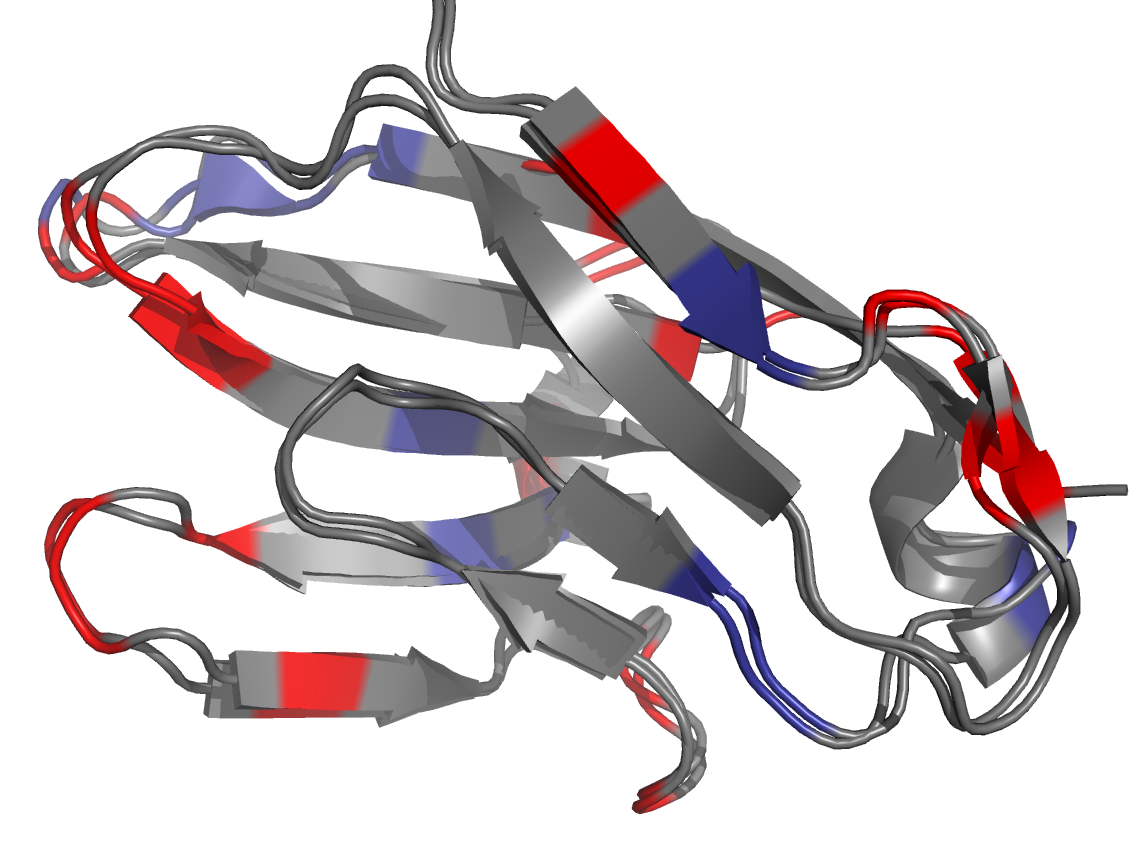
\includegraphics[width=0.58\textwidth]{02-ProtModelling/comparative/comp_72.png}}
}
 
 \mbox{
      \subfigure[High identity alignment: Alignment of 2GK2A length 111 and 2DKSA length 130. Alignment yields 80/111 (72\%)  identities and 92/111 (83\%) positives.]{
      
\begin{minipage}{0.9\textwidth}
\begin{tiny}
\tt %makes the font fixed-width so that all the columns line-up
\begin{tabbing}

\ \ \ \ \ \ \=1\ \ \ \ \ \ \ \ 10\ \ \ \ \ \ \ \ 20\ \ \ \ \ \ \ \ 30\ \ \ \ \ \ \ \ 40\ \ \ \ \ \ \ \ 50\ \ \ \ \ \ \ \ 60\ \ \ \ \ \ \ \ 70\ \ \ \ \ \ \ \ 80\ \ \ \ \ \ \ \ 90\ \ \ \ \ \ \ \ 100\ \ \ \ \ \ \ \ 111 \\
\>|\ \ \ .\ \ \ \ |\ \ \ \ .\ \ \ \ |\ \ \ \ .\ \ \ \ |\ \ \ \ .\ \ \ \ |\ \ \ \ .\ \ \ \ |\ \ \ \ .\ \ \ \ |\ \ \ \ .\ \ \ \ |\ \ \ \ .\ \ \ \ |\ \ \ \ .\ \ \ \ |\ \ \ \ .\ \ \ \ |\ \ \ \ .\ \ \ \ .| \\
2GK2A\ \textcolor{black}{SG}\textcolor{Red}{G}\textcolor{black}{AQLT}\textcolor{Red}{T}\textcolor{black}{E}\textcolor{RoyalBlue}{SM}\textcolor{black}{P}\textcolor{Red}{F}\textcolor{black}{N}\textcolor{Red}{V}\textcolor{black}{AEGKEVLLLVHNLPQ}\textcolor{Red}{QLF}\textcolor{black}{GY}\textcolor{RoyalBlue}{S}\textcolor{black}{WYKGE}\textcolor{Red}{R}\textcolor{black}{VD}\textcolor{Red}{G}\textcolor{black}{NR}\textcolor{RoyalBlue}{Q}\textcolor{black}{I}\textcolor{RoyalBlue}{V}\textcolor{black}{GY}\textcolor{Red}{A}\textcolor{black}{I}\textcolor{Red}{GT}\textcolor{black}{QQ}\textcolor{Red}{A}\textcolor{black}{TPGPA}\textcolor{Red}{N}\textcolor{black}{S}\textcolor{Red}{G}\textcolor{black}{RETIYPNASLL}\textcolor{RoyalBlue}{IQ}\textcolor{black}{NVT}\textcolor{RoyalBlue}{Q}\textcolor{black}{NDTG}\textcolor{Red}{F}\textcolor{black}{YTLQVIK}\textcolor{Red}{S}\textcolor{RoyalBlue}{D}\textcolor{black}{L}\textcolor{RoyalBlue}{VN}\textcolor{black}{EE}\textcolor{Red}{A}\textcolor{black}{TGQF}\textcolor{Red}{H}\textcolor{black}{VY}
\\
\>\textcolor{black}{SG}\textcolor{Red}{\ }\textcolor{black}{AQLT}\textcolor{Red}{\ }\textcolor{black}{E}\textcolor{RoyalBlue}{++}\textcolor{black}{P}\textcolor{Red}{\ }\textcolor{black}{N}\textcolor{Red}{\ }\textcolor{black}{AEGKEVLLLVHNLPQ}\textcolor{Red}{\ \ \ }\textcolor{black}{GY}\textcolor{RoyalBlue}{+}\textcolor{black}{WYKGE}\textcolor{Red}{\ }\textcolor{black}{VD}\textcolor{Red}{\ }\textcolor{black}{NR}\textcolor{RoyalBlue}{+}\textcolor{black}{I}\textcolor{RoyalBlue}{+}\textcolor{black}{GY}\textcolor{Red}{\ }\textcolor{black}{I}\textcolor{Red}{\ \ }\textcolor{black}{QQ}\textcolor{Red}{\ }\textcolor{black}{TPGPA}\textcolor{Red}{\ }\textcolor{black}{S}\textcolor{Red}{\ }\textcolor{black}{RETIYPNASLL}\textcolor{RoyalBlue}{++}\textcolor{black}{NVT}\textcolor{RoyalBlue}{+}\textcolor{black}{NDTG}\textcolor{Red}{\ }\textcolor{black}{YTLQVIK}\textcolor{Red}{\ }\textcolor{RoyalBlue}{+}\textcolor{black}{L}\textcolor{RoyalBlue}{++}\textcolor{black}{EE}\textcolor{Red}{\ }\textcolor{black}{TGQF}\textcolor{Red}{\ }\textcolor{black}{V+} \\
2DKSA\ \textcolor{black}{SG}\textcolor{Red}{T}\textcolor{black}{AQLT}\textcolor{Red}{I}\textcolor{black}{E}\textcolor{RoyalBlue}{AV}\textcolor{black}{P}\textcolor{Red}{S}\textcolor{black}{N}\textcolor{Red}{A}\textcolor{black}{AEGKEVLLLVHNLPQ}\textcolor{Red}{DPR}\textcolor{black}{GY}\textcolor{RoyalBlue}{N}\textcolor{black}{WYKGE}\textcolor{Red}{T}\textcolor{black}{VD}\textcolor{Red}{A}\textcolor{black}{NR}\textcolor{RoyalBlue}{R}\textcolor{black}{I}\textcolor{RoyalBlue}{I}\textcolor{black}{GY}\textcolor{Red}{V}\textcolor{black}{I}\textcolor{Red}{SN}\textcolor{black}{QQ}\textcolor{Red}{I}\textcolor{black}{TPGPA}\textcolor{Red}{Y}\textcolor{black}{S}\textcolor{Red}{N}\textcolor{black}{RETIYPNASLL}\textcolor{RoyalBlue}{MR}\textcolor{black}{NVT}\textcolor{RoyalBlue}{R}\textcolor{black}{NDTG}\textcolor{Red}{S}\textcolor{black}{YTLQVIK}\textcolor{Red}{L}\textcolor{RoyalBlue}{N}\textcolor{black}{L}\textcolor{RoyalBlue}{MS}\textcolor{black}{EE}\textcolor{Red}{V}\textcolor{black}{TGQF}\textcolor{Red}{S}\textcolor{black}{VH}
\\
\>|\ \ \ |\ \ \ \ .\ \ \ \ |\ \ \ \ .\ \ \ \ |\ \ \ \ .\ \ \ \ |\ \ \ \ .\ \ \ \ |\ \ \ \ .\ \ \ \ |\ \ \ \ .\ \ \ \ |\ \ \ \ .\ \ \ \ |\ \ \ \ .\ \ \ \ |\ \ \ \ .\ \ \ \ |\ \ \ \ .\ \ \ \ |\ \ \ \ .| \\
\>6\ \ \ 10\ \ \ \ \ \ \ \ 20\ \ \ \ \ \ \ \ 30\ \ \ \ \ \ \ \ 40\ \ \ \ \ \ \ \ 50\ \ \ \ \ \ \ \ 60\ \ \ \ \ \ \ \ 70\ \ \ \ \ \ \ \ 80\ \ \ \ \ \ \ \ 90\ \ \ \ \ \ \ \ 100\ \ \ \ \ \ \ 110\ \ \ 116


\end{tabbing}
\end{tiny}
\end{minipage}
}}

\vspace{0.4cm}

\mbox{
      \subfigure[Structural alignment of 2GK2A to 1L6ZA.]%
      {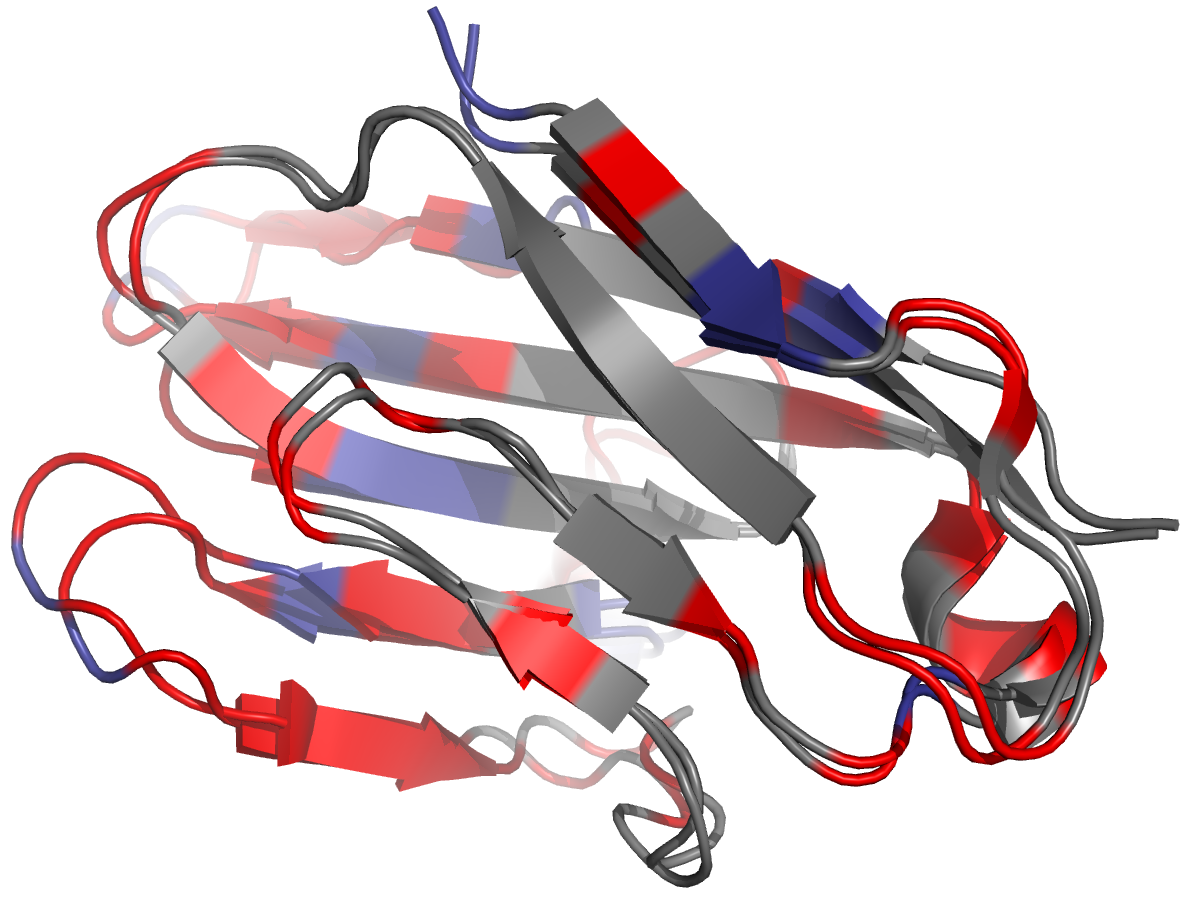
\includegraphics[width=0.58\textwidth]{02-ProtModelling/comparative/comp_42.png}}
}

\mbox{
      \subfigure[Low identity alignment: Alignment of 2GK2A length 111 and 1L6ZA length 107. Alignment yields 45/107 (42\%) identities and 62/107 (58\%)
positives.]{

\begin{minipage}{0.2\textwidth}
\begin{tiny}
\tt %makes the font fixed-width so that all the columns line-up
\begin{tabbing}

\ \ \ \ \ \ \=5\ \ \ \ 10\ \ \ \ \ \ \ \ 20\ \ \ \ \ \ \ \ 30\ \ \ \ \ \ \ \ 40\ \ \ \ \ \ \ \ 50\ \ \ \ \ \ \ \ 60\ \ \ \ \ \ \ \ 70\ \ \ \ \ \ \ \ 80\ \ \ \ \ \ \ \ 90\ \ \ \ \ \ \ \ 100\ \ \ \ \ \ \ \ 111\\\
\>|\ \ \ \ |\ \ \ \ .\ \ \ \ |\ \ \ \ .\ \ \ \ |\ \ \ \ .\ \ \ \ |\ \ \ \ .\ \ \ \ |\ \ \ \ .\ \ \ \ |\ \ \ \ .\ \ \ \ |\ \ \ \ .\ \ \ \ |\ \ \ \ .\ \ \ \ |\ \ \ \ .\ \ \ \ |\ \ \ \ .\ \ \ \ .|\\
2GK2A\ \textcolor{RoyalBlue}{QL}\textcolor{black}{T}\textcolor{red}{T}\textcolor{black}{E}\textcolor{RoyalBlue}{SM}\textcolor{black}{P}\textcolor{red}{FN}\textcolor{black}{VAE}\textcolor{red}{GKE}\textcolor{black}{VLLLVHNLP}\textcolor{red}{QQ}\textcolor{black}{L}\textcolor{red}{FG}\textcolor{RoyalBlue}{YS}\textcolor{black}{WYKG}\textcolor{red}{ERVDG}\textcolor{RoyalBlue}{NRQ}\textcolor{black}{I}\textcolor{red}{VG}\textcolor{RoyalBlue}{Y}\textcolor{red}{AIG}\textcolor{RoyalBlue}{T}\textcolor{red}{QQATP}\textcolor{black}{G}\textcolor{red}{P}\textcolor{black}{A}\textcolor{red}{N}\textcolor{black}{SGRE}\textcolor{red}{T}\textcolor{black}{IY}\textcolor{red}{P}\textcolor{black}{N}\textcolor{red}{A}\textcolor{black}{SLL}\textcolor{red}{I}\textcolor{black}{Q}\textcolor{red}{N}\textcolor{RoyalBlue}{V}\textcolor{black}{T}\textcolor{red}{QN}\textcolor{black}{D}\textcolor{red}{T}\textcolor{black}{G}\textcolor{red}{F}\textcolor{black}{YTL}\textcolor{red}{Q}\textcolor{RoyalBlue}{V}\textcolor{red}{IKS}\textcolor{RoyalBlue}{D}\textcolor{red}{LVNE}\textcolor{RoyalBlue}{E}\textcolor{black}{AT}\textcolor{red}{G}\textcolor{RoyalBlue}{Q}\textcolor{black}{FHVY}\\
\>\textcolor{RoyalBlue}{++}\textcolor{black}{T}\textcolor{red}{\ }\textcolor{black}{E}\textcolor{RoyalBlue}{++}\textcolor{black}{P}\textcolor{red}{\ \ }\textcolor{black}{VAE}\textcolor{red}{\ \ \ }\textcolor{black}{VLLLVHNLP}\textcolor{red}{\ \ }\textcolor{black}{L}\textcolor{red}{\ \ }\textcolor{RoyalBlue}{++}\textcolor{black}{WYKG}\textcolor{red}{\ \ \ \ \ }\textcolor{RoyalBlue}{+++}\textcolor{black}{I}\textcolor{red}{\ \ }\textcolor{RoyalBlue}{+}\textcolor{red}{\ \ \ }\textcolor{RoyalBlue}{+}\textcolor{red}{\ \ \ \ \ }\textcolor{black}{G}\textcolor{red}{\ }\textcolor{black}{A}\textcolor{red}{\ }\textcolor{black}{SGRE}\textcolor{red}{\ }\textcolor{black}{IY}\textcolor{red}{\ }\textcolor{black}{N}\textcolor{red}{\ }\textcolor{black}{SLL}\textcolor{red}{\ }\textcolor{black}{Q}\textcolor{red}{\ }\textcolor{RoyalBlue}{+}\textcolor{black}{T}\textcolor{red}{\ \ }\textcolor{black}{D}\textcolor{red}{\ }\textcolor{black}{G}\textcolor{red}{\ }\textcolor{black}{YTL}\textcolor{red}{\ }\textcolor{RoyalBlue}{+}\textcolor{red}{\ \ \ }\textcolor{RoyalBlue}{+}\textcolor{red}{\ \ \ \ }\textcolor{RoyalBlue}{+}\textcolor{black}{AT}\textcolor{red}{\ }\textcolor{RoyalBlue}{+}\textcolor{black}{FHV+}\\
1L6ZA\ \textcolor{RoyalBlue}{EV}\textcolor{black}{T}\textcolor{red}{I}\textcolor{black}{E}\textcolor{RoyalBlue}{AV}\textcolor{black}{P}\textcolor{red}{PQ}\textcolor{black}{VAE}\textcolor{red}{DNN}\textcolor{black}{VLLLVHNLP}\textcolor{red}{LA}\textcolor{black}{L}\textcolor{red}{GA}\textcolor{RoyalBlue}{FA}\textcolor{black}{WYKG}\textcolor{red}{NTTAI}\textcolor{RoyalBlue}{DKE}\textcolor{black}{I}\textcolor{red}{AR}\textcolor{RoyalBlue}{F}\textcolor{red}{VPN}\textcolor{RoyalBlue}{S}\textcolor{red}{NMNFT}\textcolor{black}{G}\textcolor{red}{Q}\textcolor{black}{A}\textcolor{red}{Y}\textcolor{black}{SGRE}\textcolor{red}{I}\textcolor{black}{IY}\textcolor{red}{S}\textcolor{black}{N}\textcolor{red}{G}\textcolor{black}{SLL}\textcolor{red}{F}\textcolor{black}{Q}\textcolor{red}{M}\textcolor{RoyalBlue}{I}\textcolor{black}{T}\textcolor{red}{MK}\textcolor{black}{D}\textcolor{red}{M}\textcolor{black}{G}\textcolor{red}{V}\textcolor{black}{YTL}\textcolor{red}{D}\textcolor{RoyalBlue}{M}\textcolor{red}{TDE}\textcolor{RoyalBlue}{N}\textcolor{red}{YRRT}\textcolor{RoyalBlue}{Q}\textcolor{black}{AT}\textcolor{red}{V}\textcolor{RoyalBlue}{R}\textcolor{black}{FHVH}\\
\>|\ \ \ .\ \ \ \ |\ \ \ \ .\ \ \ \ |\ \ \ \ .\ \ \ \ |\ \ \ \ .\ \ \ \ |\ \ \ \ .\ \ \ \ |\ \ \ \ .\ \ \ \ |\ \ \ \ .\ \ \ \ |\ \ \ \ .\ \ \ \ |\ \ \ \ .\ \ \ \ |\ \ \ \ .\ \ \ \ |\ \ \ \ .\ |\\\
\>1\ \ \ \ \ \ \ \ 10\ \ \ \ \ \ \ \ 20\ \ \ \ \ \ \ \ 30\ \ \ \ \ \ \ \ 40\ \ \ \ \ \ \ \ 50\ \ \ \ \ \ \ \ 60\ \ \ \ \ \ \ \ 70\ \ \ \ \ \ \ \ 80\ \ \ \ \ \ \ \ 90\ \ \ \ \ \ \ \ 100\ \ \ \ 107\\

\end{tabbing}
\end{tiny}
\end{minipage}
}}

\vspace{0.5cm}

\caption[Sequence:Structure relationships between homologous templates]{Sequence$\to$Structure relationships between typical homologous templates. The sequence alignment
was generated using a PDB  service. Colours in the sequence alignment correspond to those in the structural alignment. Structural images created using \pymolV.
}
\label{fig:intro:seqstrucrelationship}

\end{center}
\end{figure}

So, nature is inherently economical; once a stable protein fold has evolved, the same structural motif is then often reused, augmented with new function.
The implication is therefore that, as long as one can find at least one high-quality representative structure for each of a limited number
of protein folds, the representative member(s) of each fold can be used in the \emph{prediction} of any undefined structures which share high sequence
identity.




\subsubsection{Template Availability}

The future is promising for the scope of available 
modelling templates. \xray\ crystallography is traditionally only applied to proteins of direct interest. However, due to increasing use of template-based
modelling techniques, there has been a recent drive to use targeted high-throughput crystallography to get at least one representative structure for each basic
fold type\cite{COMPCHEM:Gou2002}. This process will inevitably increase the diversity of available templates and allow template-based modelling to be performed on a greater variety of proteins and with a higher degree of accuracy.


\subsubsection{Threading and Fold Recognition}

Fold recognition\cite{SIMULATION:FoldRecognition} and threading\cite{SIMULATION:Threading} methods involve the mapping of sequences onto known protein folds.  The
most recent methods use sequence$\to$structure profiles derived from multiple
sequence alignments in order to enhance
the mapping process\cite{SIMULATION:GenThreader,SIMULATION:Karplus2001}. By scanning fold libraries it is possible to identify structures which are potentially compatible with the target sequence.
This evaluation is performed independent of the sequence identity; only the
energetic stability of a given sequence within a given fold is scored. 
The
most energetically stable folds then progress into further stages of refinement.
Typically, the model represents only the spatially conserved positions of the fold, often the protein core, so the production of an all-atom protein model  requires further stages of surface loop placement and side-chain packing.

Protein threading has a role in protein structure prediction that is intermediate between comparative modelling and \abinitio\ prediction. Using threading, models can be produced for candidate sequences where there
is no high sequence identity template and can often identify the correct
fold; the main problem with these methods is that they often fail to correctly
align the sequence within the fold, resulting in erroneous final models\cite{METHOD:CASP:FoldRecognition}.

\subsubsection{Comparative Modelling}


Comparative or homology modelling is the process by which a 3D model structure is produced, for a chosen candidate sequence, using information
from one or more structural templates which share significant sequence identity. 
Enhancement of comparative modelling is a focus of the work presented in this thesis. The
specific issues in the field of comparative
modelling as a whole are discussed further in section \ref{section:comparative_modelling}
following the introduction of other prerequisite modelling considerations.


\subsubsection{Template-based Modelling Summary}

In summary, template-based modelling provides a shortcut to true \abinitio\ modelling. By effectively tightly pre-defining the topology of the candidate sequence of interest using structural templates, conformational space is vastly reduced and calculation detail can be increased. This not only results
in more accurate models of higher confidence, but also means that models can be generated for larger structures. 

The downside of the use of templates is that structures with novel folds
cannot be predicted. In addition, the models produced by this kind of modelling
say nothing about the pathways, forces and overall energetics of the folding
process itself.
Although template-based modelling will never be a complete solution for \insilico\ protein folding, multi-domain-sized proteins can be modelled using current levels of computer power, making this group of modelling techniques especially
valuable to the molecular biologist.









\section{Protein Representation}
\label{section:protein_rep}

The great dilemma for protein simulation is the balance between the complexity of the protein representation and forcefield used to describe a protein system and the coverage of the conformational search. This balance must be addressed within the scope of available computer power.
Increasing the complexity of the \forcefield, with the aim of increasing its discriminatory power, not only increases the time required to search conformational space, but also usually results in a more difficult search due to the increased number of competing
energy minima. 


The converse is a reduction in the complexity of the protein model, which can reduce the time required to evaluate the chosen scoring functions. This can be accomplished via a reduction in number of particles by using unified residues. For example, the \textsc{Unres}\cite{COMPCHEM:Cza2004,COMPCHEM:Liw97} and \raft\cite{COMPCHEM:Gib2001} representations use centroids to represent the backbone and \sidechain\ atoms. Alternatively, the various \mbox{united-atom}\cite{COMPCHEM:Der99,COMPCHEM:Osg99} representations also aim to reduce the number of particles in the system by amalgamating hydrogen atoms with their parent heavy-atom. Methods accomplishing reduction in conformational space have varied hugely, ranging from simplified coordinate lattice models\cite{COMPCHEM:Hin92,COMPCHEM:Hin94,COMPCHEM:Kol94,COMPCHEM:Cov94} over discretising the allowed values for the conformational variables (such as torsion angles\cite{COMPCHEM:Gib2001}) or by using polypeptide fragment libraries\cite{METHOD:Rosetta,METHOD:Rosetta:CASP3}. \Sidechain\ freedom can also be reduced by using rotamer libraries to represent highly populated conformational sub-states.

The problem with the use of low complexity methods is that oversimplification of protein geometry may severely compromise the specificity required to discriminate between native and non-native compact conformations, especially in the densely packed core regions, and may be partially responsible for the failure of such models with increasing protein size. Equally, over-restriction of backbone geometries may not enable the molecule to fold co-operatively in a way that maximises the attractive energies between interacting bodies, due to the restricted freedom of movement. This could partially account for the significant deterioration in the ability of models with restricted geometry to describe structures which are rich in \bstrands\ in comparison to their representation of \mbox{\al-helical} structure -- The energetic stability of \mbox{\be-structure} is much more sensitive to angle variations\cite{COMPCHEM:Gib2001}.

Continued development of a successful reduced
representation\cite{COMPCHEM:Gib2001} and its application to loop modelling is described further in chapter \ref{chapter:reduced_rep}.
As such representations are incapable of \emph{precisely} representing the native state,
but only native-like states, chapter \ref{chapter:prearcus} goes on to describe the refinement of viable conformations into final all-atom models.






\section{Energy Functions}
\label{section:protmodel:energy_functions}

Protein \forcefields\ play a crucial role in all avenues of protein modelling
including protein dynamics simulations, protein design calculations, modelling
of both protein:protein and protein:ligand interactions and in protein structure prediction. There is a wealth of current research dedicated to improving the ability of protein \forcefields\ to describe the free energy landscape of proteins; signified by a host of recent reviews\cite{FORCEFIELD:REVIEW:1,FORCEFIELD:REVIEW:2,FORCEFIELD:REVIEW:3,FORCEFIELD:REVIEW:4}.

Each of these simulation classes is clearly attempting to model the same underlying
physical laws, therefore theoretically, if infinite computer power were available, a single perfect \forcefield\ would be sufficient for all protein simulation. Critically however, computer power is finite and so, depending on the specifics of a given simulation, the chosen \forcefield(s) must strike the optimal balance between calculation detail and speed. For example, a docking
\forcefield\ is required to rapidly screen many millions of small compounds \insilico\ and therefore favours speed of execution. Even the most detailed docking \forcefields\ are usually only concerned with soft-sphere sterics, crude empirical hydrogen bonding and  desolvation terms within the active
site. By contrast, to make predictions of physical quantities like   folding rates, detailed protein folding simulations  are required. These  must employ the highest quality physical models and use  explicit solvent at the expense of calculation speed. 

Forcefields for protein structure prediction reside between these two poles.
The crucial difference is that these algorithms are not required to simulate
protein kinetics, but are instead required to distinguish between a  number of distinct
conformational states. The chosen \forcefield\ is typically required to screen many thousands of these potential protein models, but also needs to describe the native state with sufficient clarity to discriminate against protein-like competing minima.



It is important that the chosen forcefield successfully models, directly or indirectly, the hydrophobic effect, electrostatics, solvation effects and hydrogen bonding.
 Frequently in protein modelling, forcefields based upon statistical potentials, derived from the PDB, or simplified physico-chemical \forcefields\ are used. Molecular mechanics \forcefields,  particularly when augmented with implicit solvation models, provide increasingly successful physics-based energetic evaluations. Historically they have not been extensively used, due to their relative computational expense, but are now beginning to play an  important role.

\subsection{Molecular Mechanics Forcefields}

In a traditional molecular mechanics \forcefield, the potential energy of the system is broken down into a defined number of individual components. The sum of
these components is  used to represent the energetics of each competing conformation on the folding landscape. 

Equation \ref{eqn:intro:mmff:A} shows how the energy of the system is split between bonded and non-bonded terms.
Each of the terms shown is usually referred to as a potential energy function,
or PEF, as they aim to describe the potential as opposed to the kinetic energy
of the system. The parameters for the the various PEFs of molecular mechanics
forcefields are derived from many sources including both quantum mechanical calculations and thermodynamic, crystallographic and spectroscopic data for a wide range of systems\cite{FORCEFIELD:REVIEW:3,FORCEFIELD:REVIEW:4}.

\begin{equation}
\Delta E_\mathrm{System} = \Delta E_\mathrm{Bonded} + \Delta E_\mathrm{Non-Bonded}
\label{eqn:intro:mmff:A}
\end{equation}

The most popular ``Third Generation'' molecular mechanics forcefields are \amber\cite{FORCEFIELD:AMBER,COMPCHEM:Pon2003},
\charmm\cite{FORCEFIELD:CHARMM}, \textsc{Opls}\cite{COMPCHEM:OPLS,COMPCHEM:OPLS:B} and \textsc{Gromos}\cite{COMPCHEM:GROMOS}. Each implementation is based on the
same broad principles but varies in its specific details. These are all available in multiple versions and differing atomic detail.

\subsubsection{Bonded Energy Terms}
\label{section:protmodel:bondedterms}

Equation \ref{eqn:intro:mmff:B} shows the standard bonded \forcefield\ terms
which are concerned with the geometry of covalently linked atoms. Unfavourable energy is associated with deviations from optimal molecular geometry. Bond lengths, angles between bonded atoms and torsion angles along each bond are all constrained near populated equilibrium values using separate PEFs. 

Each covalently linked atom pair is joined by a bond; the energetics of 
which are usually
approximated
using a simple harmonic potential with an associated force constant. Each angle between these bonds
is also harmonically
restrained  to a given equilibrium value. Torsions on the other hand are modelled using a periodic function which aims to model the energetic barriers found during bond rotation. 

Bonded energies vary greatly with even small deviations away from equilibrium
values and are therefore meaningless unless a given protein conformation
is first locally energy minimized. As a simplification, some algorithms choose to work only with idealised geometry and therefore can completely ignore
both the bond and angle terms.

\begin{equation}
\Delta E_\mathrm{Bonded} = \Delta E_\mathrm{Bonds} + \Delta E_\mathrm{Angles} + \Delta E_\mathrm{Torsions}
\label{eqn:intro:mmff:B}
\end{equation}

\subsubsection{Non-Bonded Energy Terms}

Equation \ref{eqn:intro:mmff:C} defines
the non-bonded \forcefield\ terms, which are concerned with the interactions between atoms which are not covalently linked. These  PEFs  usually include
both the Lenard-Jones potential and Couloumbic interactions.
In order for the aqueous solvent to be represented without explicitly modelling water molecules, implicit solvent terms are often included to define solvent interactions. 

\begin{equation}
\Delta E_\mathrm{Non-Bonded} = \Delta E_\mathrm{Lenard-Jones} + \Delta E_\mathrm{Coulombic} + \Delta E_\mathrm{Solvation}
\label{eqn:intro:mmff:C}
\end{equation}

The Lennard-Jones potential, given in equation \ref{eqn:intro:mmff:lj}, aims to represent both weakly attractive \vdw\ (VDW)  forces and the strongly repulsive forces caused by orbital overlap. $\epsilon$ and $\sigma$ in this case are atom-dependent parameters. The functional form of the Lenard-Jones potential is very sensitive to atomic
radius overlap. This is sometimes replaced
by a soft-sphere alternative, which is more forgiving during protein simulation.

\begin{equation}
\Delta E_\mathrm{Lenard-Jones} = 4 \epsilon \left[  \left( \frac{\sigma}{r} \right)^{12} - \left( \frac{\sigma}{r} \right)^{6} \right]
\label{eqn:intro:mmff:lj}
\end{equation}

Couloumbic or 
electrostatic interactions are usually described by Coulomb's law using equation \ref{eqn:intro:mmff:couloumb}, in which  $\epsilon_0$ is the permittivity of free space, $\epsilon$ is the dielectric constant, $r_\mathrm{ij}$ is the separation of atoms $i$ and $j$ in angstroms and $q_i$ and $q_j$ are charges of atom $i$ and atom $j$ respectively.

\begin{equation}
\Delta E_\mathrm{Coulombic} = \sum^N_\mathrm{i=1} \sum^N_\mathrm{j=i+1} \frac{1}{4 \pi \epsilon_0 } \frac{q_iq_j}{r_\mathrm{ij}\epsilon}
\label{eqn:intro:mmff:couloumb}
\end{equation}

In the context of protein modelling, bonded forcefield terms can be satisfied by many different protein conformations.
 The real discriminatory power of a \forcefield\ must be derived from the treatment of hydrogen bonding, long range electrostatic effects and the highly complicated effects of solvent interaction. Protein modelling  is therefore critically linked to the representation of the electrostatic and solvation components of the forcefield.
The ultimate  driving force of the non-bonded components is to produce compact protein structures in a way that also satisfies molecular geometry.    

Modern molecular mechanics PEFs model hydrogen bonds within the careful balance
between the electrostatic and and Lennard-Jones interactions. Some alternatives
 implementations\ utilise specialised hydrogen bonding terms which can involve \emph{explicit} directional specificity.

\subsubsection{Implicit Solvation}
\label{section:protmodel:implicit_solvation}

Real globular proteins, of course, reside permanently within aqueous solvent. Good
atomic models for water, termed explicit solvent, do exist and are commonly used in high-detail MD simulations. Explicit solvent however poses a number of difficulties for protein structure prediction algorithms. Firstly, \forcefield\ calculations often involve pairwise comparisons between all atoms in the
system. If water is included
in the simulation  it introduces a large number of additional atoms and in
turn hugely increases the number of pairwise calculations.
Secondly, some prediction algorithms utilise  large changes in the protein conformation, meaning that after each move, the water must be re-equilibrated in order to make an energy calculation. Finally computing the energy of a protein embedded in explicit
solvent molecules is time consuming, because the energy
must be averaged over many solvent configurations. All these problems are avoided by treating the solvent as a time-averaged continuum, also known as an implicit solvent model. 

Equation \ref{eqn:intro:impsol} describes the basis of the implicit solvation model whereby the solvent is modelled as a continuous bulk property. The energetics between the protein and the solvent continuum are usually divided into two components. 

\begin{equation}
\begin{array}{ll}
\Delta E_\mathrm{Solvation} 
& = \Delta E_\mathrm{Vacuum \to Water} \\
& = \Delta E_\mathrm{Polarisation} + \underbrace{ \Delta E_\mathrm{VDW} + \Delta E_\mathrm{Cavity}}_{\mathrm{Surface~term}}
\\
& \approx \Delta E_\mathrm{Polarisation} + \displaystyle \sum^n_\mathrm{i=1} \sigma_i
\mathrm{SASA}_i \\
\end{array}
\label{eqn:intro:impsol}
\end{equation}

$\Delta E_\mathrm{Polarisation}$ is the solvation polarisation energy which accounts for the interaction of the partial charges
within the protein and dipoles which these charges induce within the bulk
solvent. The result of this is that atomic charges closer to the protein surface are more favourable and show weaker apparent charge-charge interactions with each other. The solvation polarisation energy is usually calculated using the generalised Born method and describes interaction of atomic charges.
The usual formulation of this PEFs is described further in the following section.

$\Delta E_\mathrm{VDW} + \Delta E_\mathrm{Cavity}$ accounts for the hydrophobic effect, describing the interfacial free energy of uncharged protein with the solvent continuum. The surface term consists of two basic components. The first is the favourable VDW interaction energy with the solvent. The second is an unfavourable cavity term which calculates an entropic cost for ordering solvent at the solute$\to$solvent interface upon the formation of the solvent cavity. It is assumed that these effects are strongest on the first shell of water around the solvent and therefore the energy would be proportional to the solvent-accessible surface area (SASA)\cite{FORCEFIELD:SASA}. For each atom ($a_i$), the surface constant $\sigma_i$
is  multiplied by $\mathrm{SASA}_i$ in the calculation.
Alternative pairwise methods are available which are computationally
more efficient but give less accurate results\cite{FORCEFIELD:POPS}.

 
\subsubsection{The Generalised Born Formulation}
\label{section:intro:gb}

In implicit models, the solvent is usually treated as a time-average
continuum with bulk solvent properties. The electrostatic interactions of a protein in solvent
are modelled as a set of point charges,  placed inside a low-dielectric cavity, surrounded
by a high-dielectric medium. In such a model, the Poisson-Boltzmann (PB) equation (\ref{eqn:intro:poisson})
relates the electrostatic potential ($\phi$) and the dielectric constant vector (r).   $\nabla$ (dell)\ is the differential operator.

\begin{equation}
\nabla.\epsilon\left(r\right)\nabla\phi\left(r\right)=\rho\left(r\right)
\label{eqn:intro:poisson}
\end{equation}

The PB equation, for all but the simplest systems, must be solved numerically 
via the finite difference method.
This places point charges and their associated radii of influence on a grid of finely spaced points, where the finer the grid, the more accurate the end result. This numerical technique makes any calculations using the PB equation
intrinsically slow.
The generalised Born\cite{FORCEFIELD:GB} (GB) model has recently received considerable attention as a rapid approximation to the numerical solution of the PB equation. Because the GB model is intrinsically based on the same underlying continuum approximation as used in PB theory, its accuracy is naturally assessed by comparison with the PB results. 

The GB model calculates the electrostatic polarisation free energy caused
by the movement of a protein solute into aqueous medium. This involves a change in the inherent polarisability of the medium, \ie the ability for the molecules to align themselves with the reaction field. This is described by a dielectric value ($\epsilon$), which accounts for the shielding of electrostatic interactions in the protein solute. As the protein moves from vacuum \mbox{($\epsilon$=1)} to aqueous solvent \mbox{($\epsilon$=80),} electrostatic effects within the solute become weaker.
The protein solute dielectric constant is poorly defined and has been assigned values between 1 and
20, although values between 2 and 4 are most common.

\begin{figure}[hptb]
\begin{eqnarray}
\Delta E_\mathrm{Polarisation} = -\left( 1 - \frac{1}{\epsilon} \right)
\sum^N_\mathrm{i=1} \sum^N_\mathrm{j=i+1} \frac{q_iq_j}{f_\mathrm{GB}}
 - \frac{1}{2}\left( 1 - \frac{1}{\epsilon} \right) \sum^N_\mathrm{i=1} \frac{q^2_i}{a_i}
\label{eqn:intro:gb} \\
f_\mathrm{GB} = \sqrt{ r^2_\mathrm{ij} + a_i a_j \exp{ \left( \frac{-r_\mathrm{ij}^2}{4a_ia_j} \right) } }
\label{eqn:intro:gb3}
\end{eqnarray}

\begin{tabular}{ll}
Where,&\\
$N$ & The total number of atoms \\
$\epsilon$ & The effective solute dielectric \\
$r_\mathrm{ij}$ & The separation of atoms i and j (\AA) \\
$q_i$ and $q_j$ & The charges of atom i and atom j respectively \\
$a_i$ and $a_j$ & The effective Born radius of atom $i$ and $j$ respectively\\
\end{tabular}

\caption{The formulation of the generalised Born equation}
\label{fig:intro:gb}

\end{figure}

The GB equation (\ref{eqn:intro:gb}) itself  has two components. The first term describes the reduction in electrostatic
energy as you move from vacuum to a dielectric medium. The second term is the favourable
energy that the system gains as its charges interact with their own induced field in the high dielectric medium. The Born radius applies to a point charge sitting at the centre of a perfectly spherical cavity whereas the effective Born radius, first introduced by Still et al.\cite{COMPCHEM:Still90}, is used for charges within non-spherical cavities. The effective Born radius of a point charge in a non-spherical cavity is equal to the Born radius of an identical ion, with the same charge and polarisation energy, in a spherical cavity. The exact methods to calculate effective
Born radii are beyond the scope of this discussion, but in essence a GB calculation using perfect effective Born radii for each atom in a given solute, will yield a very close approximation to the result of a fine-grid finite-difference PB calculation.
A host of recent advances in the precise formulation \cite{COMPCHEM:Tsu2000,COMPCHEM:Bas2000,COMPCHEM:Sim2001,FORCEFIELD:GB:ADVANCES:A,FORCEFIELD:GB:ADVANCES:B} have
resulted in GB solvation energies that now correlate extremely well with PB energies\cite{FORCEFIELD:PBGB:COMPARE}.



\subsubsection{Current Success}

Even the third generation molecular mechanics forcefield implementations, such as \ambergbsa, are still not truly reliable. It is certainly true that conformations are often found which are lower in energy than the experimentally defined native state\cite{METHOD:Plop}  and that current forcefields cannot always distinguish between native-like and protein-like decoy structures. In order to distinguish native-like conformations during protein simulation, future molecular mechanics \forcefields\ must become even more detailed, probably more extensively using quantum mechanical calculations for parametisation, although those methods are by no means mature at this stage.


\subsection{Knowledge-based and Statistical Energy Functions}


 Statistical \forcefields\ are typically derived from structural data within the
PDB. Geometric quantities and contacts are measured to obtain frequency distributions
which are averaged to derive pseudo-potentials, also known as potentials of mean force (PMFs). Commonly a single effective interaction site is chosen
for each residue, which is usually the \ca\ or \cb\ atom, from which distances
to other interaction sites are measured\cite{FORCEFIELD:REVIEW:KNOWLEDGEBASED}.

The principle advantage of statistical potentials is their raw speed. Compared
to full molecular mechanics \forcefields, even complex statistical potentials are at least an order of magnitude faster. The complementary disadvantage of statistical potentials is their great freedom of functional form causes
a highly tentative relationship to free energy. Crucially, statistical potentials derive from the finite PDB, which by its nature is a snapshot of the protein structures which are experimentally amenable.\
The PDB therefore is unlikely to accurately reflect all protein structures in nature.

One must be extremely careful not to introduce artifacts into the overall statistical potential. Many knowledge-based potentials completely disregard the context of each given
residue$\to$residue interaction.  An example of this would
be the naive observation that like-charged aspartic acid residues are found
in close proximity. Closer observation would reveal that the majority of
this probability density stems from the fact that aspartic acid residues
are frequently found in coordination with strongly positive metal ions. Thus
the interaction energy of these two \sidechains\ is required to be very different
between a metal and non-metal binding context. The issue of context is also
important for some rare, but strong interactions found in very specific contexts.
Such low-frequency observations would be given an unfavourable energy by
statistical potentials even though they are perfectly valid states. More
recent implementations attempt to remedy these issues by utilising sequence
similarity to select between multiple sets of derived potentials\cite{FORCEFIELD:Skolnick2000}.

In spite of all this, database potentials have been shown to be effective at discriminating between correct and incorrect model structures. It has also been shown that the best knowledge-based forcefields can reproduce physical quantities such the likelihood of a residue to be buried\cite{COMPCHEM:DFIRE}.



\subsection{Simplified Physico-Chemical Forcefields}

For coarse-level simulation of protein folding, it can be appropriate to
use heavily cut-down forcefields which are still based on underlying physical
principles. These physico-chemical forcefields attempt to approximate, to
varying extents, the fundamental forces between atoms and groups within the
protein. 

It is generally found that the hydrophobic effect alone is insufficient to
find protein-like conformations of small proteins. By including both hydrophobic
and polar pair-wise potentials, however, some success has been found in the
discrimination of native from non-native conformations\cite{FORCEFIELD:Huang95}. Further success has been found in the use of backbone hydrogen bonding potentials\cite{FORCEFIELD:Lee1996}. A comparatively more complex method uses similar hydrophobic and hydrogen bonding
functions with additional molecular mechanics style bonded potentials\cite{FORCEFIELD:Wallqvist1994},
however this additional level of complexity somewhat goes against the purpose
of such a reduced forcefield.



\subsection{Comparing Molecular Mechanics and Statistical Potentials}

Molecular mechanics and statistical \forcefields\ have clear advantages and
disadvantages and are ultimately suited to different roles within different
protein modelling applications. An example of where simplified physico-chemical
and statistical potentials are far more suitable is in discrimination between un-optimised structures, as molecular mechanics forcefields are exquisitely
sensitive to small changes in atom positions. Even small atomic overlap in
a given non-energy-minimised model will result in any molecular mechanics forcefield producing a meaningless energy evaluation.

The ultimate test of these very different styles of \forcefield\ is to test
them against each other, with an emphasis on the ability to distinguish between correct and incorrect structures. Recently, the \charmm\ molecular mechanics forcefield and a statistical potential
were compared for a range of conformations of the GCN4 leucine zipper\cite{FORCEFIELD:Mohanty1999}.
The study found excellent correlations both between the two forcefields and the
RMSD of each conformation to the native conformation. Neither forcefield
however identified the native state as the lowest energy conformation.

It is usual for statistical potentials to be described with somewhat arbitrary
mathematical representations which are computationally efficient and facilitate rapid calculations. Molecular mechanics \forcefields\ score protein
conformations in real units of enthalpy, by contrast statistical potentials
by nature must score based upon the frequencies of occurrence of structural
features found within high-resolution proteins structures. These frequencies
are then interpreted as free energies by assuming that the Boltzmann hypothesis\cite{FORCEFIELD:Shortle2003}
holds true, a practice that is not agreeable to all\cite{FORCEFIELD:REVIEW:KNOWLEDGEBASED}. 

An additional issue
that is related to simulation of the folding landscape is that  statistical
potentials are derived from compact folded proteins and therefore will
not be effective in representing the energetic interactions along the folding
pathway. By contrast, molecular mechanics \forcefields\ have the advantage of resting on a clear theoretical basis, allowing an in-depth analysis of energetic contributions to folding. A caveat to this is that current molecular mechanics
forcefield implementations utilise simplifications which are  necessary for tractable computing. Following further development and advances
in computer capacity, theoretical detail can be increased, thus allowing some
of these underlying simplifications to be removed. This should result in an improvement
in the discriminatory capacity of such \forcefields. 





\section{Searching Conformational Space}
\label{section:protmodel:conformational_search}

An exhaustive conformational search is impossible for all but the simplest model systems, hence
in order to find energy minima, an effective non-exhaustive search method is  required.
There are three main classes of search method, where each contains many sub-classifications:

\begin{itemize} \isep
\item 
Deterministic algorithms include build-up procedures.
Deterministic algorithms have a defined solution, thus given a particular input, they will always produce the same output.
\item
Stochastic algorithms include Monte Carlo (MC), replica
exchange, branch-and-bound and simulated
annealing. Stochastic algorithms are often faster than deterministic alternatives, however, they may return sub-optimal results.
\item
Heuristic algorithms include genetic algorithms. In general, a heuristic is a ``rule of thumb'' that guides the selection of a set of candidates at each stage of a search process. \\[-0.9cm]
\end{itemize}

If information on the dynamics of folding is required, then conceptually either MD or  MC with small conformational moves can allow the polypeptide to follow a folding pathway.
Each of these methods are briefly discussed in the following sections.

Search frustration is defined here as calculation-time spent re-exploring
the energy well of a single local minimum. The level of frustration is closely related to two important aspects of each search method.\ The first is the type and scale of conformational moves which are made to the system. Too small and the system will become frustrated, too large and nonsense structures will frequently be generated. The second aspect is
the technique which is used to escape
frustration during the search.  These aspects are discussed
in the remainder of this section where appropriate.

 

 

\subsection{Build-up}

Build-up procedures   function by joining successively long pairs of 
 polypeptide chain fragments, beginning from a single residue\cite{SIMULATION:BUILDUP}. At each stage of joining all combinations of the minima for each fragment are tested. Each fragment combination is screened for high-energy and steric overlap and subsequently minimised in \phipsi\ space. Highly similar fragments are removed to reduce redundancy. As the algorithm progresses, the chain increases in length, hence the term build-up. Such methods have been criticised
for not treating the protein as a whole during the early stages of structure
generation.

 
\subsection{Monte Carlo}

Monte Carlo (MC) searches involve pseudo-random sampling of the potential
energy surface\cite{SIMULATION:MC}. By applying a number of different types of conformational perturbations such as torsions, Cartesian coordinates, \sidechain\
rotamers as well as other more specialised moves, the conformational space
of the polypeptide chain may be explored. 

In simple MC, conformational changes are only kept if they result in an energetic
improvement.  In a system such
as protein modelling, many competing local minima exist and therefore the
conformational search is easily frustrated. This makes simple MC intrinsically inefficient, however, some common improvements which vastly improve the search process are outlined below.  

\subsubsection{The Metropolis Criterion}

The Metropolis Criterion\cite{SIMULATION:Metropolis}, shown in equation \ref{eqn:intro:metropolis}, is
used to relieve frustration in the MC\ search process by allocating a probability
that conformational changes can be made which result in an \emph{increase} in energy.
The formalism defines that decreases in energy are always accepted, whereas
an increase may be accepted at random, dependent on the Boltzman constant
($k_e$),
the magnitude of the energy increase ($\Delta E$) and the temperature of the system ($T$).
The end result is that jumps between competing local minima are more likely
as higher energy \emph{intermediate} structures may be visited.

 
\begin{equation}
P_\mathrm{accept} = \left\{ \begin{array}{ll}
 \Delta E \ge 0
  & exp^{ \left( \displaystyle \frac{- \Delta E}{k_eT} \right) } \\
\Delta E < 0
  & 1 \\
\end{array}
\right.
\label{eqn:intro:metropolis}
\end{equation}

\subsubsection{Simulated Annealing} 

Simulated annealing\cite{SIMULATION:SimulatedAnnealing} was originally formulated
as an extension to general MC, but can be utilised in all simulations where
some manner of temperature is included. The basic principle is that if
a hot dynamic system is cooled infinitely slowly to absolute zero it will cool to
the global minimum. By  cooling slowly enough, usually multiple times, possible
low energy minima can be found.


\subsubsection{Stochastic Tunneling}
\label{section:protmodel:stun}

Stochastic tunneling, or STUN\cite{SIMULATION:STUN}, aims to circumvent the slow dynamics of ill-shaped energy functions  by tunneling through energy barriers. It accomplishes this by modifying the acceptance function of standard MC  using a nonlinear
transformation to the potential energy surface. All energy wells that lie above the best minimum found so far are suppressed, so that when the simulation escapes the current well, it will not be trapped by local minima that are higher in energy. Energy wells with deeper minima are both preserved and enhanced.

 
The mathematical formalism of the STUN transform is shown in equation \ref{eqn:intro:stun},
where $f$ is the energy of the current conformation, $f_0$ is the lowest minimum encountered thus far and $\gamma$ is a
scaling factor which controls the steepness of the
transformation. 
\begin{equation}
f_\mathrm{STUN}(x) = 1-exp \left(  -\gamma(f( x) -f_{0} \right)
\label{eqn:intro:stun}
\end{equation}

STUN has been used to successfully predict
the structure of the TrpCage mini-protein\cite{SIMULATION:STUN:trpcage}.


\subsubsection{Replica Exchange}

Replica exchange, also known as parallel tempering, improves the dynamic properties of MC simulations of physical systems and is also
applicable to molecular dynamics\cite{SIMULATION:REMD}. In such
algorithms, multiple simultaneous simulations are run at different ``temperatures'',
the higher the temperature the higher the probability of making changes which
increase the energy of the system. The replica exchange occurs when the conformations
are swapped between different temperatures. In the simplest case two parallel
simulations are used where the high temperature effectively causes large deviations in conformation and the low temperature simulation is responsible for exploring around the local energy minima. By recording the low-energy minima throughout the simulation, the global
minimum of the system can potentially be found. Through careful selection of both
temperatures and number of replicas an improvement in the mixing properties of a set of MC simulations can be achieved. This provides sampling efficiency
improvements that exceed the additional computational cost of running multiple parallel simulations.




\subsection{Branch-and-Bound}

In branch-and-bound algorithms conformational space is partitioned by a quantity
such as the backbone \phipsi\ angles or inter-residue distances. For each partitioned region of space, a range of candidates are generated and screened, from which a number of areas of conformational space can be eliminated. From this selection of candidates, more potential structures can be generated. By iteratively repeating this process large regions of conformational space can be eliminated,
removing it from the search scope and increasing the efficiency of the search
process. It is critical that the method of partitioning  conformational space and
the criterion for exclusion are carefully chosen so that they do not exclude a path that will lead to the
global minimum.
It was found in a recent branch-and-bound publication that the method can
potentially be more efficient than standard Monte Carlo at finding the global energy minimum\cite{SIMULATION:BranchAndBound}.

\subsection{Genetic Algorithms}

Genetic algorithms are based on the well defined genetics  doctrine of the
evolution of species via the survival of the fittest. The method begins by the generation of a host of  different conformations, by random means or otherwise, but with significant structural diversity. These conformations are then screened for fitness via an energy criterion and a proportion are retained. These are then mutated to generate a series of children for each conformation. In true genetic algorithms there is also crossover between parent structures.
By iteratively repeating this process, multiple low energy conformations
can be generated. Genetic algorithms have had success both for generation of native-like structures for short peptides\cite{COMPCHEM:Gib2001,SIMULATION:Genetic} and helical bundles\cite{SIMULATION:Genetic:HBundle}.

Genetic algorithms become Memetic algorithms when, as part of the algorithm,
some sort of local conformational optimisation is included prior to selection of the next generation. Such local optimisation has been shown to give greater
efficiency than a standard genetic algorithm\cite{SIMULATION:Memetic}. 




\subsection{Molecular Dynamics}

Protein structure prediction is commonly unconcerned with the dynamics and
pathways of the  folding process. If such properties are required, then simulations
of protein
dynamics must be performed. The usual manner of obtaining such information
is Molecular Dynamics (MD) which simulates individual atoms using
Netwon's laws of motion.

Previous work suggests that short molecular dynamics simulations have only limited use in convergence towards the experimental structure \cite{NATIVE:Venclovas1999}.
Simulations must sample enough of the conformational space to ensure that energetic minima are found. Ergodic theory, which is assumed to be applicable to molecular dynamics, relates to the long-term behaviour and properties of dynamic systems. The theory states that if a system is sampled for a sufficient time, all the possible states of the system will be visited. An adequate duration of sampling is consequently of high importance. 

To give an idea of the required computer power, a recent high-publicity molecular dynamics simulation on the Villin Headpiece (36 amino acids) in implicit
solvent of only 1$\mu$s of folding time took $\sim$2 months CPU time on a 256-CPU Cray Supercomputer\cite{COMPCHEM:Kol98}.
Since this time, simulations of the TrpCage mini-protein (20 amino acids) have been performed
in full explicit solvent\cite{SIMULATION:TRPCAGE:EXPLICIT}. This and other recent high detail simulations can now obtain measurements in agreement
with the Nuclear Overhauser measurements obtained in NMR experiments\cite{SIMULATION:TRPCAGE:IMPLICITNMR}.
Molecular dynamic of large systems is also possible over shorter timescales. At the time of writing, some of the most impressive simulations possible are an incredible 50ns simulation of an entire satellite tobacco mosaic virus in explicit solvent totalling over 1 million atoms\cite{SIMULATION:STMV} and a 2.64 million atom simulation of the ribosome\cite{SIMULATION:Ribosome}.

Today,  bio-simulations of the protein folding process itself are only a realistic prospect for sub-domain sized chains. Significant advances have been made in the last few years and simulations are increasingly being shown to be capable of quantitative predictions such as the folding rate of a given polypeptide\cite{SIMULATION:Snow05}.
Insights into  the physical process of protein folding will ultimately come from these protein folding pathway simulations and will facilitate identification of both transition states and folding intermediates, some of which will prove to be functionally important.





  
\subsection{Conformational Space: Final Comments}

Conceptually search methods which use large conformational shifts disregard any contribution that the folding pathway itself has in determining the native
state. A theoretical issue would be if the global minimum of the system was inaccessible to the polypeptide chain during folding, but could be visited by a large artificial conformational shift during simulation. 

As has been discussed, the native state is likely to be the global free energy minimum, although conceptually this may not be the case. It is impossible, both \insilico\ and \invivo, for a polypeptide to sample
the entirety of conformational space. It is, therefore, likely that \invivo\ folding is directed by local interactions, biasing
the populations within unfolded ensemble. This implies that the native state is a deep and defined minimum, close to that of the biased unfolded ensemble.

It is also true that, given time \invitro, both amorphous aggregates and amyloid fibrils form spontaneously in protein solutions; so these competing
states must be low in free energy. Evolutionary pressure
is likely to favour polypeptide sequences which exhibit high energy
barriers to these    
 states, as they impair the activity of the cell.  Crucially, therefore, it
is likely that these states are further from the unfolded ensemble
 in conformational space, and therefore are not visited within folding timescales. 

\al-lytic protease is an interesting isolated case where, following post-translational
processing
of the polypeptide chain,  the folded state is a actually \emph{higher} in free energy than the unfolded state\cite{NATIVE:unfolded:lowerenergy}. This
case, however, does \emph{not}  break the thermodynamic hypothesis, as it is the pre-processed
state
of \al-lytic protease
is still lower in free energy than the native ensemble.
It appears that a large energetic barrier to un-folding exists for the post-processed chain, being kinetically trapped by the post-processing event and giving it  its apparent stability. This can be shown experimentally,
as
if the post-processed form is unfolded \invitro, it no longer spontaneously
refolds when folding conditions are restored.






 



\section{Comparative Modelling in Detail}
\label{section:comparative_modelling}


Comparative modelling was traditionally performed by expert human modelers whereby
the  alignment of a candidate sequence to a chosen structural template  would be manually optimised. Individual residue
mutations and packing would be performed by eye using visual tools such as
\textsc{Accelrys' Insight II}~hosted on expensive Silicon
Graphics workstations. Such expert-based modelling is often augmented by
 the appropriate use of fragment stitching tools to aid surface loop prediction; implemented in applications such as \textsc{Swiss-PDBViewer}\cite{METHOD:SWISSPDB:A,METHOD:SWISSPDB:B}. Manual modelling is
however extremely labour intensive and hinged critically on correct human judgement.

The advent of more automated responses to the modelling process  has had
a profound impact on structure prediction. When suitable templates
are available such methods are commonly
among the most successful during the modelling competition \casp\cite{METHOD:CASP6:CM}. Modern
comparative modelling utilises these automated processes, guided by human
experts where sequence identity is low. 


\subsection{Archetypes for Automated Comparative Modelling}
\label{section:protmodel:comparativemodellingarchetypes}


All comparative modelling methodologies utilise one or more structural templates at their
heart. The exact method   for structure building however varies between different
implementations. In general, all comparative modelling methodologies are not only extremely rapid, but also do not
\emph{require} human intervention (although this is still entirely possible),
and most give quantification of the certainty
of each region in the final model. 

There are three archetypal implementations
of comparative modelling:
\begin{description} \isep
\item[Rigid-body Assembly] \eg \textsc{Composer}\cite{METHOD:COMPOSER} \\
The first and still widely used approach in comparative modelling is to assemble a model from a small number of rigid bodies obtained from aligned template structures. The approach is based on the natural dissection of the protein structure into conserved core regions, variable loops that connect them and \sidechains\ that decorate the backbone. First, the template structures are selected and superimposed. Second, the ``framework'' is calculated by averaging the coordinates of the \ca\ atoms in structurally conserved regions of the template structures. Third, the backbone atoms of each core region in the target model are obtained by superposing on the framework the core segment from the template whose sequence is closest to the target. This is followed by surface loop and \sidechain\ modelling.

\item[Segment Matching] \eg \textsc{Segmod}\cite{METHOD:SEGMOD} \\
The basis of modelling by coordinate reconstruction is the finding that most hexapeptide segments of protein structure can be clustered into just 100 structurally different classes\cite{METHOD:Unger1989}. Thus, comparative models can be constructed by using a subset of atomic positions from conserved regions of the template structures as ``guiding'' positions (usually \ca), and by identifying and assembling short, all-atom segments that fit these guiding positions. The segments are obtained in a representative database of all known protein structures\cite{METHOD:SEGMOD}.

\item[Satisfaction of Spatial restraints] \eg \modeller\cite{METHOD:MODELLER}
\\
This group of methods work by minimising global deviation from a set of spatial constraints. In \modeller\ these constraints (what it terms probability density functions, or PDFs) are derived from both idealised atomic geometry (obtained from the \textsc{Charmm22}\cite{FORCEFIELD:CHARMM,COMPCHEM:MacKerell1998} molecular mechanics forcefield) and homology derived restraints (distance and dihedral angle restraints) from a statistical analysis of relationships to the template structures. This system assumes that the corresponding distances between aligned residues in the template and the target structures are similar, which is why residue correspondence in the initial sequence alignment must be correct. The allowed range of values of distance or dihedral angle deviation depends on the degree of structural variability at the corresponding position in the template structures. In the final stage approximate 3D models are refined by restrained molecular dynamics with simulated annealing in water.

\end{description}




Modelling by satisfaction of spatial restraints, is generally deemed to be the most successful of the methods. The particular strength of  restraint-satisfaction methodologies is that restraints, empirically weighted by certainty, can be derived from many diverse sources. Such sources include homology-derived restraints,
rules for secondary structure packing\cite{METHOD:Coh89}, analyses of hydrophobicity\cite{METHOD:Asz94}, correlated mutations\cite{METHOD:Tay94}, empirical potentials of mean force\cite{METHOD:Sip90}, cross-linking experiments, NMR data\cite{METHOD:COMPOSER}, image reconstruction in electron microscopy and site-directed mutagenesis\cite{METHOD:Boi93}. This allows as much information as possible to be incorporated into the final ensemble of models. These should all be compliant with all known experimental data and with more general knowledge about protein structure.



\subsection{Web-based Comparative Modelling}

As comparative modelling has become increasingly popular, many modelling programs have been converted into automated
internet-based servers. These include \textsc{Swiss-Model}\cite{METHOD:SWISSMODEL},
\textsc{3D-Jigsaw}\cite{METHOD:3DJIGSAW} and \esypred\cite{METHOD:Esypred3D}
which uses \modeller\ as its internal structure generation engine and augments
it with superior sequence alignment. 

These servers greatly simplify the modelling
process, making it accessible, even to those with limited computer experience. The caveat of this is that simulation detail must therefore be compromised in order to provide a publicly available high-throughput server
which can produce models rapidly on demand. A more accurate model can potentially be generated if a more exhaustive systematic process is utilised off-line;
for example a greater number of surface loops could be sampled, or multiple alternative alignments could be attempted. 


A recent trend that has emerged since \casp-6 is the advent of the consensus server\cite{METHOD:CASP6:CM}. This new class of server interrogates multiple modelling servers for
a given candidate sequence. As all the different servers rely on difference
primary sources of information, they yield slightly different final results. By comparing
this wealth of data and finding elements that are in agreement, it is possible to produce an even more accurate final model. An example of this system is provided by the \textsc{3D-Jury} server\cite{METHOD:3DJURY}. 





\subsection{Sequence Alignment}

A candidate sequence can be obtained from many sources, for example by sequencing a gene found to be involved in a process under study or from a genome-sequencing project. Once the sequence is obtained, homologous sequences must be found for which a 3D structure has been experimentally
resolved.
Comparative modelling starts with  sequence alignment techniques to find these homologous structures. 


The single most important factor that determines the quality of a model is the quality of the alignments that can be made. 
If the sequence alignment is incorrect, then the final model, no matter how detailed the energetic
evaluations, is guaranteed to be incorrect.
Alignment procedures only produce correct results for sequences with higher than around 30\% sequence identity\cite{NATIVE:Moult1999}. Currently, comparative
modelling applications should not be used in fully automated modes unless the sequences are so similar that the calculated alignment is likely to be correct, requiring sequence identity of 50\% or more. This requires that the poorer alignments are carefully inspected and optimized by hand before use in modelling. Moreover, several iterations of alignment and modelling may be necessary. To increase the probability that alignments are correct, information from multiple methods and multiple templates can be used and weighted by their similarity to the template.


Originally, pairwise methods were used to compare a single candidate  with a single template sequence is order to find a likely alignment. These included programs such as \textsc{Fasta}\cite{SEQUENCE:FASTA} and \textsc{Blast} (Basic Local Alignment Search Tool)\cite{SEQUENCE:BLAST}. There are now many newer methodologies that can be used to find structural templates. These include the use of many statistically based mathematical techniques such as HMM (Hidden Markov Models), Parametised Neural Nets and Support Vector Machine learning models. Sequence comparisons using multiple sequences have been shown to detect three times as many remote homologs as pairwise methods where the sequence identities of homologous pairs are less than 30\%\cite{SEQUENCE:Par98}. Two respected
alignment methods that use sequence profiles are:

\begin{description}

\item[PsiBlast\cite{SEQUENCE:PSIBLAST},] or Position-Specific Iterative \textsc{Blast}, constructs a position specific substitution matrix (PSSM) from a multiple alignment of the highest scoring hits in an initial BLAST search. Highly conserved positions receive high scores and weakly conserved positions receive scores near zero. The profile is used to perform a second (etc.) BLAST search and the results of each iteration used to refine the sequence profile. This iterative searching strategy results in increased sensitivity.

\item[ClustalW\cite{SEQUENCE:CLUSTALW}] is a general purpose multiple sequence alignment program for DNA or proteins which compares sequence profiles. It produces biologically meaningful multiple sequence alignments for divergent sequences; calculating the best match, and aligning them so that the identities, similarities and differences can be seen.

\end{description}




\subsection{Surface-Loop Refinement}

Surface loops are the most variable and least regular regions in protein structural families, exhibiting large sequence and structure changes between
homologous templates. Their modelling remains the most taxing process in comparative modelling, largely due to the lack of homology information in the template structures for these regions\cite{METHOD:CASP6:CM}. Generally all the information available for the modelling process is the location at which the loop enters and leaves the protein core, meaning that the structure of the loop must be modelled using non-comparative methodologies. Loop modelling is a large topic in itself and is covered in more detail in section \ref{section:loopmodelling}.



\subsection{\Sidechain\ Packing}

\Sidechain\ packing is commonly performed using an efficient packing algorithm
with a sufficiently fine-grained rotamer library. Rotamer definitions suffer from some of same issues as database derived loops;
primarily the scope of the underlying PDB. For most rotamer libraries, it is found that 5-30\% of \sidechains\ in crystal structures differ significantly from their closest rotamer conformations and that 6\% of the $\chi$1 or $\chi$2 values are not within $\pm$40\degree\ of any rotamer conformation. It is
therefore important to use rotamer libraries with a significant number of
alternative structures during the final stages of model refinement.




\subsection{Errors in Comparative Modelling}

The errors in comparative models are highly dependent on the degree of similarity between a given candidate and its template. Above 40\% sequence identity the majority of errors are in \sidechain\ placement and minor global \mainchain\ distortions. Between 30\% and 40\% homology, the most significant problems are caused during the creation of the rigid body of the model.  Here distortions or shifts are common in regions that do not have an equivalent segment in any of the template structures. Large insertions and deletions are common and require large regions of the template to be rebuilt. There is scope here for the use of multiple templates to define common regions of structural change. At 30\% sequence identity there is typically 1.5\AA\ RMSD following optimal superimposition the core backbone atoms\cite{NATIVE:Chothia1986}.
Below 30\%, identification of a template with enough structural similarity becomes the main problem. Below 20\% sequence alignment programs are unable to find any templates with any high degree of similarity. Finally,
if a given sequence is repeatedly randomised and compared to a sequence of the same length, with propensity weighting for the natural occurrence of amino acids, they will share between 14\% and 18\% ``homology''. This gives an effective benchmark for zero homology at about 15\% sequence identity, dependent upon
the exact sequence.

Structure refinement still proves a serious problem.  
The critical issue found during tests of final comparative models is that the model produced bears more resemblance to the template from which it is built than the experimental crystal structure of the candidate sequence. This shows that during the modelling process, the core structure of the template is not allowed to deviate in any significant way from its starting structure -- in many applications the output structure is often only generated via an  energy minimisation of the final assembled model. This procedure is typically adequate for higher homology candidate sequences where their core does not usually deviate considerably from template structures; it is however less appropriate as the sequence identity drops and changes become more pronounced. This shows a need for improvement in the local conformational space search during the modelling process. 









\section{Loop Modelling in Detail}
\label{section:loopmodelling}

Loop prediction methods are intrinsically linked to comparative modelling and are
used for SVRs where there is no template information. As the problem remains an intriguing unsolved challenge there are many methods available which attempt to solve it. 

Historically, loop modelling was a  labour-intensive interactive process. In many cases, potential fragments  which fitted
between the available anchor residues were selected \emph{manually}\cite{METHOD:FRODO}. In the case of Greer et al.\cite{METHOD:Greer1980}, who modelled
surface loops for a serine protease, each  loop was initially built using the \mainchain\
conformation of the longest
loop in a homologous template. Residue mutations were also performed manually
and any additional residues deleted. The gap was then joined by
a ``spring closing potential''. In one case, where a 17 residue insertion
was found, the loop was left undefined in their final model.  Clearly such arbitrary
methods required improvement and subsequently a multitude of a \emph{automated}
methods have been developed.

Within a given structural representation, loop modelling can be thought of as two conceptually separate and individually complex problems. The first is the method by which the vast conformational space open to a protein surface
loop is sampled. An optimal search
method will result in geometrically sensible \emph{closed} loop conformations and also sample conformations proximal to the averaged native ensemble. Secondly, the energy function(s) by which valid loop candidates are both screened and selected
must be of sufficient quality to discriminate native-like from low-energy
protein-like
conformations. 

Just as for whole protein modelling, automated loop modelling methods can be coarsely separated into the two broad groups of
database / knowledge-based and \abinitio\ methodologies, with varying shades of grey in between. These are discussed further in sections
\ref{section:loop:database} and \ref{section:loop:abinitio} respectively.





 



















\subsection{Mathematical Loop Closure}

Mathematical loop closure methods have been under development for many years. Simple numerical studies show that geometrically there are up to a maximum of eight solutions to describe the conformations of a given tri-peptide, where the backbone is described as a series of \ca\ positions constrained by the orientation of the planar peptide group\cite{METHOD:Go70}. Even at this small length, the numerical method requires sampling of space from multiple start points. The equations used are fully generalised and can be applied to longer loops, however they do not guarantee that a solution is present for a given conformation in more extreme cases. 

Exact analytical loop closure\cite{METHOD:Wed99} is possible for loops of three residues in length, with up to nine explicit backbone atoms in the definition. Using spherical geometry and polynomial equations, the loop-closure problem can be solved exactly. The number of valid loop closures can be evaluated by the method of Sturm chains, which counts the number of real roots of a polynomial. Within this mathematical definition, longer loops can be treated by three methods: by sampling enough dihedral angles to reduce the problem to a soluble loop-closure problem; by applying the loop closure algorithm hierarchically; or by dividing the chain into independently moving rigid elements that can be reconnected using loop-closure algorithms\cite{METHOD:DivideConquer}. 

In conclusion, the prediction of normal protein loop lengths cannot be simplified to an analytical  method and so requires conformational sampling. The remainder of this section looks at the various ways that sampling has been employed and some of the optimisations that have been attempted.






\subsection{Knowledge-based Methods}
\label{section:loop:database}
All knowledge-based methods function in approximately the same manner; differing in the exact methods used to filter, select and stitch candidate loops. In essence each method relies upon a database constructed by trawling the PDB to obtain viable loop structures. The resultant fragments are categorised, collated and then stored. When a loop prediction is subsequently requested, the database is consulted, fragments scored, and loop models returned, usually following stitching of the candidate(s) onto the protein body\cite{METHOD:Petra}. 




\subsubsection{The Databases}

Some of the most tried and tested protein structure prediction methods utilise  fragment databases, some of which retain sequence-specific information. By using a large enough database, the contained fragments automatically represent the local conformational propensities of a given sequence within varying protein
environments. These fragments can be found by geometry and sequence similarity before being stitched onto the protein core. Multiple databases implementations have been developed and some of the most successful, recent or popular
are shown in table \ref{table:intro:databases}.


\begin{table}[hptb]
\begin{center}
\begin{tabularx}{0.95\textwidth}{+l^X}

\toprule
\rowstyle{\bfseries}
Name & The nature of the database \\
\midrule\\[-0.2cm]

\textsc{Fread} &
The modelling method \textsc{Fread} relies upon PDB-derived databases which consist of  distances between \ca\ atoms.  The F20 database contains
1,010 protein chains with up to 20\% pairwise identity with a resolution better than 2.5\AA\cite{METHOD:FREAD:F20}.
All all non-terminal \ca\ separations are included which are separated by more than three residues and less than thirty\cite{METHOD:CODA}.\\[0.3cm]

\textsc{SLoop} &
\textsc{SLoop} is a database of super-secondary fragments containing protein loops classified by structural similarity. It contains 10,000 loops, which cluster into $\sim$560 populated classes\cite{METHOD:SLoop:A,METHOD:SLoop:B,METHOD:SLoop:C,METHOD:SLoop:D}. Loops with up to 20 residues are included.
\\[0.3cm]

\textsc{ArchDB} &
\textsc{ArchDB} is a compilation created via an automated structural classification of loops extracted from known protein structures\cite{METHOD:ArchDB:A,METHOD:ArchDB:B}.
Each loop is included with its complementary bracing structure. The categorisation
is defined by the orientation of the bracing structure, the consensus sequence profile  and the loop length. The \textsc{ArchDB} database is linked with the prediction method \textsc{ArchPred}\cite{METHOD:ArchPRED}.
\\[0.3cm]

\textsc{Lip} & 
\textsc{Lip}\cite{METHOD:LIP} is a comprehensive compilation of backbone conformations found in the PDB. It includes all protein segments of between
1 and
15 amino acids in length within the PDB, which amounts to $\sim$$10^8$
structures.  The loop length,
a 2D vector and two angles were stored to describe the orientation of the
loop with respect to the planes formed by the two anchor residues.
A rather poor resolution cutoff of 3.5\AA\ or better was used in the work.\\[0.3cm]


\bottomrule
\end{tabularx}

\caption{Some of the current popular  loop database implementations}
\label{table:intro:databases}
\end{center}
\end{table}






\subsubsection{Database Problems}

There is no guarantee that current databases derived from the PDB are a homogeneous representation of the conformational space of all  surface loops. As the length of a loop increases, there is an exponential increase in the number of possible conformations that it can adopt.
Therefore for each increase in loop length,  to cover both the additional conformational \emph{and} sequence space during modelling,
many orders of magnitude more loop  structures are required. 

Using sequence identity arguments, the authors of a recent loop database
claim that the PDB is now saturating in terms of data for loops up to 12 residues in length\cite{METHOD:DB:Fuentes2006}. This, however, is clearly still
not the case; supported by the authors'  own comment that conformations with a single representative exist within their database. Critically, it is widely accepted that it is the \emph{structural context} that is the paramount issue in determining loop conformation and not the sequence alone. A more realistic view based upon structural alignments within the PDB concludes that only
loops of up to 7 or 8 residues in length are well represented\cite{NATIVE:RepresentationOfLoopsInPDB}. The same study also concludes that as the fragment size becomes longer, loop structure
becomes more fold-specific, \ie fragments from different folds
are less likely to share similar structure. Therefore, despite rapid growth
in the PDB, 9 residue loops are unlikely to be well represented in the near future.
Accentuating the problem of database coverage is the fact that for a loop to be stitched onto the protein body, at least
two anchoring residues are needed -- this in turn means that for a 5 residue loop to be built, a 7 residue fragment is required. 

In terms of computer capacity, even if the PDB contained an exhaustive representation for
loops of up to the required 12 residues, the size of such a loop database would
become prohibitive. The size of the published LIP database amounted to 6.71\gb\ of disk space; this would increase by orders of magnitude with a truly representative
 PDB.

Finally, it has been described that ionisation states of titratable \sidechains\
 are of critical importance in determining the most energetically stable loop conformation\cite{METHOD:Plop}. Conformations in loop databases are
not annotated with such information, which is potentially of importance in
the orientation of the backbone in its original context. This is especially
true in tight turns, which were described in section \ref{section:intro:tightturns}, where it is primarily \sidechain\ interactions which stabilise unfavourable backbone conformations.




\subsubsection{Knowledge-based Scoring Functions}

There are a multitude  different techniques and parametisations of knowledge-based
methods for use in  loop modelling. Some of typical methods
are described in table \ref{table:intro:knowledgebasedloop}. In some cases
knowledge-based potentials are parametised to a particular problem such as the prediction of immunoglobulin variable domain loops. These are  useful in their own context,
but unsuitable for the generalised problem and are not discussed further.


\begin{table}[hptb]
\begin{center}
\begin{tabularx}{0.95\textwidth}{+l^X}
\toprule
\rowstyle{\bfseries}
  Name & Description \\
\midrule\\[-0.2cm]
  
\textsc{Hmmstr} & 
A  hidden Markov model (HMM) for selection of loop geometries using the I-sites library of sequence-structure motifs\cite{METHOD:Bys2000}. \textsc{Hmmstr}
importantly uses the sequence-structure motifs to score each loop structure
in its new sequence context.
\\[0.3cm]  

N/A &
Neural networks, trained on PDB fragments, have been used in the prediction of antibody
hypervariable loops\cite{METHOD:NeuralN}. Neural networks are more sensitive
to over-training than HMMs and are therefore rare within the literature.
\\[0.3cm]

\coda\ &
Loop prediction using environmentally constrained substitution tables and rule-based filters.\cite{METHOD:CODA}. \coda\ is described further in section
\ref{section:methcomp:coda}.
\\[0.3cm]

\textsc{Rapdf} &
\textsc{Rapdf} is around two orders of magnitude faster than using the molecular
mechanics energy-function \ambergbsa. It has however been shown to be significantly less accurate for loop prediction.
\\[0.3cm]

\textsc{DLoop} & 
\textsc{DLoop} implements the \dfire\cite{COMPCHEM:DFIRE} potential in the context of loop structure prediction\cite{COMPCHEM:Zha2004}. \dfire\ focuses on breaking the tendency of typical knowledge-based functions to violate or ignore basic physical principles. This is achieved by accounting for the significantly different compositions at the surface, core, and interface
of proteins. It was shown that this highly successful potential can quantitatively reproduce the likelihood of a residue to be buried and the stability scale
of amino acids derived from mutation data.
\\[0.3cm]

\bottomrule
\end{tabularx}
\caption{Common knowledge-based scoring methods.}
\label{table:intro:knowledgebasedloop}
\end{center}
\end{table}



\subsection{Concluding Remarks}

In spite of the difficulties associated with  database-derived methods, they are used with significant success for modelling shorter loops of up to $\sim$7 residues in length. This is due to the good representation of the fragment sequence space in PDB fragments of this size. All these fragments represent real low-energy structures and therefore have a built-in bias towards the local structural propensity of a given loop sequence; explaining the success for short loops. The defining
feature of all knowledge-based and database methods is rapid speed of calculation.
As such, they are especially suited to high-throughput modelling.












\subsection{\AbInitio\ Methods}
\label{section:loop:abinitio}

All \abinitio\ loop modelling methods take a given protein core with two anchor residue definitions and a loop sequence to be built between them. A build operation is then conducted which positions the loop atoms between the two anchors. This can occur in the presence of other protein body atoms or in isolation in which case the loop structure must subsequently be attached to the protein body. Following the build process the loop candidates must be scored in some way. Some methods cluster multiple representations together in order to find the best representative from a similar collection of successful structures. Some methods focus on the efficient generation of backbone conformations and must be augmented with additional functionality in order to provide \sidechain\ conformations.


The term \abinitio\ covers a wide variety of methodologies.  These include random tweak\cite{METHOD:Xia2002,METHOD:AntibodyB,METHOD:Antibody}, analytical methods\cite{METHOD:Kinematic,METHOD:Wed99,METHOD:DivideConquer}, constraint optimisation\cite{METHOD:RapperB}, scaling relaxation\cite{METHOD:Zhe94}, robotics derived algorithms\cite{METHOD:Robotics} and a contact-matrix method\cite{METHOD:Gal2001}. Other more computationally expensive methods sample low-energy conformations using detailed all-atom energy calculations derived from either molecular or statistical mechanics. This class of methods includes those based on Molecular Dynamics\cite{METHOD:Bru87}, Monte Carlo\cite{METHOD:Abagyan94,METHOD:Zha97}  and simulated annealing\cite{METHOD:Fis2000}. In addition to basic molecular dynamics, some methods attempt to increase sampling efficiency by using soft-core non-bonded potentials\cite{METHOD:Levitt1983,METHOD:Tappura2001}. 

A comparison of \abinitio\ loop modelling methodologies was performed
for this thesis. Individual applications that were involved in this comparison
are presented and critically compared in more detail in chapter \ref{chapter:methods}. 

\subsection{Successful Traits for Loop Modelling}

Throughout the literature a number of important factors which define successful modelling methods have emerged:

\begin{itemize} \isep
\item 
It has been shown that inclusion of the surrounding protein body atoms is essential to discriminate native-like from non-native models\cite{METHOD:CLOOP}.
\item 
The long-standing debate as to wether knowledge-based potentials are suitable
in determining native-like conformations continues. Many authors of successful methods\cite{METHOD:Plop,METHOD:RapperA} have commented that, especially for longer loops, realistic physico-chemical forcefields qualitatively outperform standard knowledge-based potentials\cite{METHOD:Modloop}.
By contrast, the authors of the most successful knowledge-based potentials conclude
superiority over physico-chemical forcefields\cite{COMPCHEM:Zha2004}. What is undisputed is that knowledge-based
potentials are both rapidly calculated, less sensitive to poor
steric conformations than molecular mechanics forcefields and inherently suitable for filtering poor structural conformations.
\item
Many of the latest and most successful methods utilise a hierarchical modelling
approach with each successive level feeding candidate structures to the next
for further refinement\cite{METHOD:Plop,METHOD:RapperB}.
Computational modelling is always a compromise between the detail of the energetic calculation and the
scope of the conformational search within the constraints of available computer power. These  successful  methods ensure that the relevant level of detail is invoked at each process level. This ensures that enough of conformational space is sampled, poor candidates are screened early in the modelling process and that sufficient loop candidates are evaluated on the most detailed energy functions. This in turn will yield the best chance of obtaining near-native loop conformations.
\end{itemize}


\subsection{Applications for Loop Modelling}

As has been discussed, loop prediction is intimately entwined with the process
of comparative modelling. Surface loops are often critically  important to function and indeed most active sites are formed by the \sidechains\
of surface loops. As such, both molecular  interaction and active site design or re-engineering will become a real possibility
as loop prediction matures. Such sites can include those for protein/ligand interaction, the hyper-variable loops of antibodies\cite{METHOD:Antibody} and the long loops of G-Protein-Coupled Receptors (GPCRs)\cite{METHOD:AP:GPCR1,METHOD:AP:GPCR2}.






\section{Final Comments}

Protein structure prediction is becoming increasingly important in many diverse
fields of work including both drug and catalyst design. Whilst experimental structure determination is the gold standard, current methods are still labour intensive and slow. Worse still, many classes of proteins remain difficult
to deal with experimentally, such as those which can not be expressed at high concentration, those with a tendency to aggregate and the very substantial class of membrane proteins. For these structures, \insilico\ modelling methodologies
are a tempting alternative, including the most successful current method of
comparative modelling. As advances are made to  the comparative
modelling methodology, confidence in the models produced will grow, and so the
method should become increasingly accepted. A critical element of comparative modelling is the refinement of surface loops for which little structural information is present in template structures; this is the focus of the work in the following chapters of the dissertation.
   %  2. Introducing Protein Modelling
\chapter{Software Development}
\label{chapter:software}

\begin{quote}
``The strange flavour of AI work is that people try to put together long sets of rules in strict formalisms which tell inflexible machines how to be flexible.'' \\ 
--- \textit{Douglas Hofstadter}
\end{quote}

\section{Introduction and Aims}

The primary aim of this work is the development of enhanced methods for modelling short sections of polypeptide, usually at the surface of proteins. The main use of such a protocol is as a tool in the more general process of comparative modelling. 
It is almost impossible to know \textit{a priori} whether or not a novel methodology will show promise when applied to a given real-world problem. Often the only way of verifying a given approach is the process of trial and error. It is clearly of benefit to be able to rapidly experiment with multiple different algorithms in order to pragmatically find the best solution -- as Linus Pauling once said, ``The best way to have a good idea is to have lots of ideas''. For various reasons discussed in this chapter, traditional software engineering concepts do not lend themselves well to this process; mainly because such software requires a clearly predefined implementation before development begins. 

The solution to these concerns is the creation of a molecular simulation framework, or ``toolkit'', that allows the user to experiment with new algorithms. Novel algorithms can be created by the recombination of well-established and fundamental building-blocks, without the need to constantly start from the beginning. It is therefore crucial to have an adaptable foundation and modularity is paramount. 

Mike Tyka and I felt, at the beginning of our PhDs, that such a framework was not available to us. A fruitful collaboration quickly ensued, which has ultimately resulted in the creation of a novel simulation engine, currently combining over seven man-years of development. This engine focuses on rapid algorithm development, both for ourselves and for new researchers in the future. It is now in a state to be of real use, representing a significant advance over traditional implementations.

In addition to the simulation engine, it is also important to implement facilities for the extraction and subsequent processing of data from the PDB and other experimental sources. To this end, a second framework has also been developed in parallel with  a different overall aim to that of the first. This framework lacks simulation capabilities, but is instead concerned with error-tolerant data extraction and supplies many convenient methods for subsequent processing and visualisation.  It again focuses on the primary principles of flexibility and extensibility and the current implementation is used throughout this work. Additional tools for 3D molecular visualisation and data graphing have been developed which rely upon the common underlying framework.

The aim of this chapter is threefold. Firstly current coding practices are discussed to orient the reader with respect to recent software engineering advances. These advances are used throughout the software developed for this thesis. Secondly, existing third-party simulation frameworks are discussed. Finally, the simulation and data extraction engines are discussed in turn. Initially an overview of the implementation of each framework is presented. Potential roles and typical usage of the software are then discussed. Finally the core code elements are discussed. It is not the intension here to provide a manual for any of the software; as such documentation is available in a more comprehensive form online from the group website. The development snapshot of the source code at the time of writing is included on an enclosed CD.


\section{Modern Coding Practice} 

Before discussing the specifics of the software developed for this thesis, it seems pertinent to briefly discuss modern coding standards and techniques.
It is hoped that this will illustrate how the developed code-bases  relate
to cutting-edge software development.
 
 
\subsection{Compiled Source Code}

The fundamental language of a modern computer is \emph{machine code}; essentially
a short list of basic operations that can be performed on data. Such language, to
a human, is incredibly verbose, cryptic and generally  difficult to understand. As such,
higher level languages have been developed which are human readable, but
can be \emph{compiled} into machine code. Modern compilers are well tailored
to this practice and generate highly efficient machine code from the
corresponding human readable source code. This results in what is termed an executable,
or binary, which can then be invoked on a host computer to manipulate data.

A choice of computer languages exist, all of which are best suited to different applications.
Historically, procedural languages have been extensively used throughout the academic environment.
Through experience within the software industry, a number of difficulties with this paradigm have been
found and are discussed briefly below. To address these issues, modern applications
are written under a new paradigm termed object oriented programming
(OOP). This is extensively used throughout this work and is also discussed below.  
 
\subsection{Procedural Languages}

The procedural programming paradigm is based upon the concept of top-down functional decomposition -- essentially, breaking
a problem down into a collection of procedural calls, conditional statements and primitive data arrays.
Procedural calls are also termed function calls, but should not to be confused with mathematical functions; each one performs a list of defined operations on data. After a procedural program is initiated, based on user input, a defined execution path ensues.

Common procedural languages used in the academic environment are Fortran and C, which have been around since the 1950s and 1970s respectively. As C is a more recent language
it less common in the academic environment. Both languages exhibit a minimalistic design with tightly defined language structure.\ This results in code which can be highly optimised
by the compiler and thus run in less time. This makes both languages especially suited to numerically intensive computation and scientific computing.  
Importantly, over the abilities of Fortran-77, C facilitates very powerful low-level access to computer memory.

\subsection{Object Oriented Languages}

Today, software applications are larger and more complex than ever before. The majority
of the cost of a modern software is in its maintenance --  fixing errors, modification, adding options -- often costing twice that of the
original software development. As such, it is critical that software frameworks
never ``re-invent the wheel''; meaning that overlapping functionality should be minimised and that standardised libraries, techniques and algorithms should be used wherever possible. This new emphasis on modularity and reusability fits neatly within the object oriented programming (OOP)  paradigm. 

In OOP, the conceptual currency of the language is the \emph{object}, as opposed to the procedural call. An object, put simply, is a logical grouping of data and functions which manipulate that data. Each object has a conceptually tightly-defined purpose and if designed properly can be \emph{reused}. As each of these reusable objects can be independently tested, the development process can be simplified. 
What is ultimately gained, is that programs can be developed much more quickly, with a greater likelihood of correct behaviour.


\section{Solving Difficulties in Legacy Frameworks}
\label{section:software:proceduralprobs}

It has long been realised, not only in science but in the software industry
as a whole, that classic programming techniques have some fundamental limitations.
In this section, we discuss some of the difficulties that arise from
the use of the procedural paradigm and how OOP attempts to solve some of these
problems. This is by no means intended as a comprehensive review of OOP practice,
as such literature is available in abundance, but is intended as a brief
overview for potential advantages of OOP in the scientific software environment. All the enhancements described here are used throughout this work.

\subsection{Problem 1: Global Data Scope}

The following code-snippet, listing \ref{listing:software:prob1}, shows a tiny but typical procedural application which accomplishes a given task based on user input. In this simple example all is well; the user is given just two options and the application behaves as expected, reporting the user-chosen code-path and the resultant calculated energy. This procedural paradigm, however, begins to fail as   one wants to give the user additional options and application size
increases.  

\lstset{language=CSharp}
\begin{lstlisting}[float, caption={Example procedural pseudo-code (C-like).}, label=listing:software:prob1] 
double energy; // A global variable storing the energy of the system

// A fixed-length global array of double precision floating point numbers holding atomic radii
double radius[100]; 

void setupRadii( int codePath ); // A function to fill the radius array based on the code path

// Global forcefield function calls which calculate the energy of the system using
// the global radius array, and stores the result in the global variable `energy'.
void forcefieldA(); // A forcefield calculation, coded by person A
void forcefieldB(); // A forcefield calculation, coded by person B

// Our program begins with a call to the function main()
void main(int pathID)
{
        setupRadii( pathID ); // Setup the radii dependent on the user specified code path

        if( pathID == 1 ) { forcefieldA(); } // Run forcefieldA
        else if( pathID == 2 ) { forcefieldB(); } // Run forcefieldB
        else 
        {
            printf{"Please enter either option 1 or 2. You entered %d",pathID);
            return; // Exit early without printing the energy
        }

        // Report the execution path and calculated energy to the user
        printf("Mode %d yields an energy of %f kcal/mol", pathID, energy );

        return; // We completed successfully
}

\end{lstlisting}

The main concern in this implementation, is that both forcefield() calls use the same global data array to store radii. What if each forcefield calculation requires different atomic radii? An easy solution might be to simply create two independent and persistent global arrays of radii, radiusA and radiusB. However, this practise quickly becomes impractical as the total number of forcefield functions increases. As all data is global, it can be modified by any function at any time, which makes tracking down errors intrinsically difficult. Each array must be separately maintained, typographical errors can result in the modification of the wrong data array \emph{without warning} and many of the arrays will be completely redundant for multiple code-paths.
Naive array duplication is clearly not a good solution.


Instead, as in listing \ref{listing:software:prob1}, we could call a setup() function prior to each forcefield() call, with each function reliant on the same global data array. Each function then has specific requirements about when and where it can be called and what \emph{must} be called beforehand. Critically, it is common for this practise to result in incompatibilities, especially when different code-paths are implemented by different people. In addition,
when a user requests an unusual selection of application parameters, strange and undefined effects can occur. The application itself must therefore be carefully designed and documented; but this process \emph{requires} specialist knowledge of the entire code-base, not just for the developer, but in the worst cases also the \emph{user}.

Even if one is very careful, with multiple developers, this process rapidly becomes unmanageable and so classical procedural applications are usually small and limited to a single well-defined task. This, however, results in applications with overlapping functionality. For these separate applications to interact, they must communicate via common-format input and output files, coordinated by shell scripts; a process that is again  messy and error-prone.  Many small scientific applications actually share a good deal of common ground, such as how to read structural data from a file, but each one must be maintained and upgraded separately when new features or performance enhancements are created.


\subsection{Solution 1: Class-based Architecture}

 We have already mentioned that in OOP, the fundamental building-block of an application is
the \emph{object}. Put simply, an \emph{object} is a humanised grouping of data. Each object is self-contained and combines both data and functions into one neat package. The technical terminology is that an \emph{object} is as an instance of a \emph{class} -- a \emph{class}
being the blueprint for a given type of \emph{object}. The rules for the interrelationships between various objects are subsequently enforced by the compiler. 

\subsubsection{Class Scope}

Procedural applications essentially only have global and local \emph{scope} -- scope simply defines the lifetime of data. Global
scope data persists from initiation to termination of the application as a whole and can be changed at any time by any function. Local scope data,
defined at the start of a function call, expires  when the function terminates.
OOP\ languages extend this by adding class scope, where the data is only accessible via the  object to which it belongs and exists for the lifetime of that object.

Not all persistent data and associated functions need to be accessed globally and hence their interface should be tightly defined;
only a function that needs access to data should be granted such access. Importantly, class scope  data and functions can be made \emph{private}, which means that they can only be accessed from within the object itself.  This greatly reduces software development time and maintenance cost because there are fewer potential sources of logical errors -- the compiler will catch data-access logic errors at compile-time, preventing their propagation to run-time.

\subsubsection{An Example}

Let us revisit the example put forward in listing \ref{listing:software:prob1}.
In the new version, shown in listing \ref{listing:software:sol1}, we introduce
the ForcefieldA class, which conceptually embodies everything to do with  implementation-A of a forcefield as a single self-contained unit. Importantly,  the radius array and setupRadii() call are class-scope and made private; meaning that they can only be used by functions belonging to ForcefieldA. By contrast, print() and evaluate() represent the \emph{public interface} and can be called at any time, but only by client functions that possess a reference to a ForcefieldA object. 

\lstset{language=CSharp}
\begin{lstlisting}[float, caption={Example  OOP pseudo-code (C++).}, label=listing:software:sol1] 
// The *abstract* concept of a forcefield is embodied by a class structure
// Implementation A
class ForcefieldA
{
public:
        // The class constructor is called automatically when an instance of ForcefieldA is made
        ForcefieldA()        
        {
            setupRadii();    // the object configures itself when it is created
        }

        double evaluate();   // Returns the current energy
        void   print();      // Prints the current energy, calling 'evaluate' internally
private:
        void   setupRadii(); // Fill the radius array based on the code path
        double radius[100];  // Private radius array belonging to this instance
};

// Implementation B
class ForcefieldB
{
public:
        // The class constructor is called automatically when an instance of ForcefieldB is made
        ForcefieldB()
        {
            setupRadii();    // the object configures itself when it is created
        }
        double evaluate();   // returns the current energy
        void   print();      // prints the current energy, calling 'evaluate' internally
private:
        void   setupRadii(); // Fill the radius array based on the code path
        double radius[100];  // Private radius array belonging to this instance
};

// Our program begins with a call to the function main()
void main(int pathID)
{
        if( pathID == 1 ) 
        { 
                ForcefieldA ff; // Here we create an instance of ForcefieldA
                ff.print();     // and ask it to print its energy
        }
        else if( pathID == 2 ) 
        { 
                ForcefieldB ff; // Here we create an instance of ForcefieldB
                ff.print();     // and ask it to print its energy
        }
        else 
        {
            printf{"Please enter either option 1 or 2. You entered %d",pathID);
            return; // Exit early without printing the energy
        }
        return; // We completed successfully
}

\end{lstlisting}

Therefore, by using objects, we solve problem 1. Firstly there is predominantly no longer any need for global data.
Each data element is tightly associated with its parent object, and can \emph{only}
be accessed through that object.
Secondly, we no longer have the difficulty that ForcefieldA can be, in any way, influenced
by the actions ForcefieldB. Finally, there is no waste, because a class instance is only created in memory when it is needed.
 
\subsubsection{Additional Benefits}
 
Importantly, as
each class tightly defines only its public interface, classes also provide intrinsic
modularity in the code. This means that the internal implementation of a given feature can be changed
at a later date, usually to increase efficiency or correct errors. As long as the interface itself doesn't change,  no other
code which depends on it will be broken. This means that testing is
confined to a single class and reduces maintenance time. Finally, after a
set of complementary class interfaces are agreed, a single developer can work on the implementation
of each interface, simplifying and accelerating the development process.   






\subsection{Problem 2: Code Duplication and Stagnation}

In procedural programming, tasks such as sorting a list of atomic Cartesian coordinates are usually performed by a single specialised function which looks at independent
x, y and z arrays. The same underlying algorithm
however may also be used elsewhere in the code that simply sorts a list of integers
or floating point numbers. Critically, each \emph{requires} a separate function, all of which must be separately maintained
but in essence implement the same underlying algorithm but for different data structures. What is needed is a way of allowing
a single copy of the algorithm to work on multiple different but analogous data types. 



\subsection{Solution 2A: Class Inheritance}
\label{section:software:inheritance}

We have already discussed how conceptual groups of data and functions can be combined within a single object. Many of these objects actually share a good deal of logic. As has been discussed, code duplication should be avoided at all costs, to
decrease the maintenance burden for a given application.  A mechanism for sharing common functionality between objects is a technique
called \emph{inheritance}, illustrated in listing \ref{listing:software:inheritance}.

\lstset{language=CSharp}
\begin{lstlisting}[float, caption={Class inheritance.}, label=listing:software:inheritance] 
class Position // A class describing a Cartesian position
{
public:
    double x;
    double y;
    double z;
    
    void moveToOrigin();                // Move to 0,0,0
    void moveTo( Position& newPos );    // Move to a position in Cartesian space
    void moveBy( Position& newPos );    // Displace by a Cartesian vector
    void rotate( RotationMatrix& rot ); // Rotate in space using this matrix
    void print();                       // Print the current location
}

class Atom : public Position // Derive Atom from Position
{
public:
   int index;
   std::string name;
   double radius;
}

// A function which does something to a position in space
void manipulatePosition( Position& pos );

void main()
{
    Atom a;                // Create an atom
    a.x += 12.0;           // Add 12 to the X coordinate of Atom a
    a.moveToOrigin();      // Move the atom to the origin
    manipulatePosition(a); // Perfectly legal, as an atom IS also a position
}

\end{lstlisting}

Take, for example, an atom. In a typical implementation of a molecular simulation, an atom is essentially
a position in Cartesian space with additional properties, such as a  radius, numeric index or name. For geometric manipulation, the kind of things one wants to perform on an atom are essentially the same as for any other position in space. What is needed is a way of giving an atom the same properties
as a position without duplicating the underlying code. To do this we \emph{derive} \textsl{Atom}
from \textsl{Position}, and subsequently \textsl{Atom} gains all the properties of a Cartesian position; consequently, \textsl{Position} is the \emph{base class} of \textsl{Atom}.

This has a number of important implications. Firstly, any function that can
work on a \textsl{Position}, such as sorting, can now also work on an \textsl{Atom}. This requires
no code duplication. Secondly, when we upgrade Position with new features or a
performance enhancement, \textsl{Atom} implicitly gains these new abilities.  Finally,
and perhaps most importantly, such abstractions are very intuitive to the user -- one expects to be able to move an \textsl{Atom} in space and therefore treat
it as a \textsl{Position}.

\subsection{Solution 2B: Template Meta-Programming}
\label{section:software:templates}

A recent and extremely useful language development is template meta-programming.
Meta-programming is essentially code which creates further tailored code on demand. Say for example we need a function that adds together all the
elements in an array and we have integer, floating-point and position arrays.
In standard procedural and indeed more basic OOP languages, one would have to create three
specialised functions which essentially do the same thing, but on different
data types. Listing \ref{listing:software:template} shows how templates allow the programmer to tell the compiler to \emph{automatically}
create these functions.  This means that common algorithms need only be coded and maintained once and can be re-used between multiple problems. 

\lstset{language=C++}
\begin{lstlisting}[float, caption={Template meta-programming.}, label=listing:software:template] 
// The traditional method; copy and paste the algorithm.
double   sumArray( double* data,   int count ); 
int      sumArray( int* data,      int count );
Position sumArray( Position* data, int count );

// The template form, whereby T is essentially a wildcard. The compiler automatically duplicates
// the function body and replaces T with each type that is actually used within the application.
// The end result is that the three functions are defined by just one general function, 
// In this case, 1/3 of the effort is thus required.
<template T>
T sumArray( T* data, int count )
{
   T sum = 0;
   for( int i = 0; i < count; i++ ) // iterate over all data
       sum += data[i]; // add data element `i' and sum, storing the result in sum
       
   return sum;
}
\end{lstlisting}

It should be noted that the same effect may be obtained with weakly-typed and dynamic languages such as Perl and Python respectively, whereby interpretation of a given code line
occurs at runtime rather
than at compile time. It is worth noting, however, that such practice comes
with an associated performance penalty and so is less suitable for use with high performance
scientific code. An additional problem with these languages is that, as machine code is
generated at runtime, some logic checks cannot be performed by the compiler.
This means that some types of code error can be retained until further along the development path. 







\subsection{Problem 3: Static Memory Allocation}

Fortran-77 does not allow dynamic memory allocation, requiring that the
size of all arrays be pre-defined at compile time. The programmer decides
that the largest molecular system that will be imported will contain 10,000
atoms and sets this limit. As is usual, some time later someone has a more powerful
computer and wants to simulate a larger system -- they can't. If the application
source code is still available and has been well designed, these limits
can easily be increased and the application recompiled. However, this results in multiple
versions of the application, where the new version will no longer execute on older computers. In addition, not all of the static arrays will be used to capacity,
resulting in significant waste for the original smaller molecular systems and requires higher specification hardware to facilitate
execution.
Furthermore, the addressing of larger memory ranges inevitable has an associated performance penalty, as larger data arrays are less likely to remain within the limited CPU level 1 and level 2 caches.

\subsection{Solution 3A: Dynamic Memory Allocation}

Compared to Fortran-77, newer procedural languages like C are more powerful as they allow dynamic memory allocation. Thus, the issue is not directly with procedural languages  \mbox{\textit{per se}}, but relates more to the limits imposed by the use of legacy languages and compilers. In listing \ref{listing:software:memory} we show how memory could dynamically be created in C to hold a set of $n$ Cartesian coordinates.
The principle advantage of this is that, at any given point, only the memory that is needed has been allocated. The disadvantage is that this memory then needs to be \emph{managed} by the programmer, a task which is non-trivial and error prone.
\lstset{language=C++}
\begin{lstlisting}[float, caption={Static versus dynamic memory allocation.}, label=listing:software:memory] 
// The legacy way - a static, fixed-length structure of arrays
#define SYSTEM_SIZE 100;
double x[SYSTEM_SIZE];
double y[SYSTEM_SIZE];
double z[SYSTEM_SIZE];

// The C way - a dynamic array of structures
typedef struct pos_data
{
    double x;
    double y;
    double z;
} Position;

Position* makePositions( int n )
{
    // Allocate new memory to contain the new atoms
    // and return the address of the allocated memory.
    // This memory *must* be freed later...
    Position* atoms = (Position*) malloc( sizeof(Position) * n ); 
    return atoms;
}
\end{lstlisting}



\subsection{Solution 3B: Container Classes}

Modern OOP takes dynamic memory allocation a step further by making
it more user friendly, powerful and less error-prone with the advent of container
classes; illustrated in listing \ref{listing:software:containerclass}.
These are used frequently in OOP programs when the programmer requires \emph{dynamic} arrays of a given type of object. There 
are different types of container for different purposes, including lists, stacks (first
in, first out) and queues (first in, last out).
Each container class utilises templates (section \ref{section:software:templates}) and can, therefore, be created for any object type. 
All containers classes automatically manage their internal memory and come with built-in functionalities, allowing
them to be dynamic -- they can change size during program flow, having elements deleted or maybe duplicated.

\lstset{language=C++}
\begin{lstlisting}[float, caption={The power of container classes.}, label=listing:software:containerclass] 
void print( std::vector<double>& data )
{
    printf("Data: "); // Print a header
    for( size_t i = 0; i < data.size(); i++ ) // data knows its own array length via size()
    {
        printf("%3.1f, ",data[i]); // print data element i to 1 decimal place
    }
    printf("\n"); // New line
}

void main()
{
    std::vector<double> myData; // A container for double precision floating point numbers
    myData.push_back(4.0);
    myData.push_back(9.0); // Add some data to the container
    myData.push_back(1.0);
 
    std::vector<double> myDataB; // Create a second container
    myDataB = myData; // Copy all the data from myData into myDataB

    print( myDataB ); // Print the copied data
    myDataB.erase(myDataB.begin()+1); // Erase the second container element (element 1)
    print( myDataB ); // Print the data following manipulation
    myDataB.insert( myDataB.begin(), 8.3 ); // Insert 8.3 at the beginning
    print( myDataB ); // Prove its worked
    print( myData ); // Show the original array remains unchanged

}

// Application Output:
// Data: 4.0, 9.0, 1.0, 
// Data: 4.0, 1.0, 
// Data: 8.3, 4.0, 1.0, 
// Data: 4.0, 9.0, 1.0,
\end{lstlisting}

All these highly optimised and well planned container classes are provided as standard with all modern OOP languages. In \CPP\ they are provided within the standard template library (STL). Importantly, every programmer will be instantly familiar with these classes, reducing  the learning-curve for any new developers. 

A second major advantage of container classes is the built-in provision for common every-day algorithms, such as sorting, illustrated in listing \ref{listing:software:sort}. In algorithms like sorting, the bulk of the logic is constant no matter what data is being operated on.  Traditionally, each data type required its own function with duplication of the underlying algorithm. In the example, std::sort() is provided by the STL; the only logic that is missing is exactly what makes a \textgreater\ b. The programmer provides this in what is called a \emph{predicate} -- in the context of sorting, quite simply a function that returns true if $a>b$. This vastly reduces code duplication and means that any data can be sorted by any criteria with a trivial amount of new code.\   
 

\lstset{language=C++}
\begin{lstlisting}[float, caption={Sorting.}, label=listing:software:sort] 
// Legacy!
void sortAtoms(); // Single purpose function
void sortAtoms( Position* p, int count ); // Function to sort ANY position array

// Modern -- separate the sort algorithm from the element comparison
bool testByXCoordinate( Position& a, Position& b ) // returns true if a > b
{
   // Sort based upon the X coordinate alone
   return a.x > b.x;
}
void sortAtoms(std::vector<Position>& pos )
{
    // Sort position vector via a predicate.
    std::sort( pos.begin(), pos.end(), testByXCoordinate );
}
\end{lstlisting}

As the standard container classes come with such a wealth of advantages and are both heavily-optimised and error-tested, they should be used at the core of all new applications based upon the OOP\ paradigm.











\subsection{Problem 4: Managing Program Flow}
\label{section:software:prob4progflow}

Listing \ref{listing:software:prob1} can be further used to illustrate an issue with
the chosen user interface. What if we want to execute both forcefieldA() and forcefieldB() because they describe different but complementary energetic aspects? In this simple case, a new code path must be created which calls both in turn and sums their results. The difficulty with this is when an application has been in development for a decade, it is likely to have  hundreds of different possible forcefield calls, the combinatorial management of which is likely to be very difficult.

Most scientific applications are controlled by the user via the
command line, whereby the executable is started with a series of arguments
which affect program flow. The difficulty with this model is that a user
interface for each implemented
code feature must be explicitly defined; usually by some sort of alpha-numerical
flag read from the command line or a file.
Each of these must be separately maintained and documented, but also means
that a significant amount of code is dedicated to reading and checking
these flags before execution begins.

In order to facilitate greater flexibility of execution, the creators of some well established applications such as the \amber\ and \charmm\ molecular
mechanics frameworks, have even implemented their own internal scripting languages. These, whilst
very useful, are not as powerful as a full blown programming language, allowing
only simple features like incrementation of counters, conditional statements
and the notoriously error-prone goto statement. An example of a \charmm\ script for a simple energy minimisation is shown in listing \ref{listing:software:charmm}.

\lstset{language=charmm}
\begin{lstlisting}[float, caption={Example \charmm\ script to perform an
energy minimisation, adapted from official \charmm\ documentation. The standard use of highly abbreviated commands is detrimental to the user experience; for example ``CTOFnb'' means nothing to the user without searching though complementary documentation.}, label=listing:software:charmm] 
! Read in Topology and  Parameter files
open unit 1 card read name top_all22_prot.inp 
read RTF card unit 1
close unit 1

open unit 1 card read name par_all22_prot.inp 
read PARA card unit 1
close unit 1

! Read sequence from the PDB coordinate file
open unit 1 card read name myprotein.pdb 
read sequ pdb unit 1 
close unit 1

! now generate the PSF and also the IC table (SETU keyword)
generate prot setu

! build in hydrogens if using a crystal structure
hbuild sele all end

! build in missing coordinates using values in
! the parameter set
ic fill
ic para
ic build

! non bonded interaction
NBONd  CUTNb  15.0  CTONnb  14.0  CTOFnb  14.5  SWITch  VSWItch CDIElectric EPSilon  1.0

! minimise structure
energy
mini sd nsteps 500 nprint 50
energy

stop
\end{lstlisting}



If multiple simulations are required to be integrated, it is common for these
to be managed by crude customised shell scripts. These often use error-prone
calls, with limited sanity-checks, to parse data from the output files of one application and from it somehow create an input file for the next application. 




\subsection{Solution 4: Integrated Scripting}
\label{section:software:integratedscripting}

A fairly recent innovation, to aid in the export of the features in a software framework to the user, is the integration of an existing independently-developed scripting engine. These languages, such as Python and TCL are incredibly powerful languages
in their own right. By presenting entire  classes from an underlying code-base directly to the user,
robust and easy-to-develop applications can  be written quickly. This removes all
need for explicit command line flags and associated setup functions, with the caveat that underlying
code-base is required to be very well designed to be intelligible to the end-user. Such a system is used in this work, and is discussed in more detail in section \ref{section:software:pd} 










\section{The Future of Algorithm Design}
Moore's Law\cite{COMP:Moore65} is the empirical observation first coined in 1965, stating that the number of transistors on a basic cost integrated circuit boards roughly doubles every 18-24 months. It is assumed that the number of transistors correlates with chip complexity and therefore the number of floating point operations per second (FLOPS)  for a given processor. This law has held true from 1965 until the present day, however in terms of single processor cores, Moore's Law has begun to fail. Due to the physical limitations of the electrical properties of silicone, making smaller transistors in the future will not
be possible. In order to maintain the same rate of performance increase CPU manufacturers are now releasing multi-core processors; a trend that is likely to continue for the foreseeable future. 

In the light of this transition toward multi-core architectures, within the high performance computation (HPC) community,  several prominent spokespeople\footnote{Dr. John Gustafson, ClearSpeed Technology Ltd.} have begun to raise certain issues over current algorithm design and choice of implementation. New software implementations  \emph{must} take full advantage of parallel processing techniques in order to remain competitive in performance on the latest architectures. This involves utilising parallel processing application programmers interfaces (APIs) such as OpenMP, MPI and the new
Threading Building Blocks from Intel.\ These can also be used in combination with new hardware technologies such as dedicated co-processor boards now hosted in several HPC institutions, including Blue Crystal at the University of Bristol.

A second important issue is that within current architectures a processor now takes hundreds of times longer to read a number from main memory than it does to perform arithmetic on it with fifteen-digit accuracy. Reading data from a hard drive takes orders of magnitude more time again. This intrinsically means that methods using large-scale pre-calculated
databases waste available resources as the CPU lays dormant waiting for IO access. With that in mind, high-detail all-atom calculations are becoming more computationally feasible for use as evaluators in protein structure prediction -- such calculations require comparatively little data access,
but require \emph{significant} processing power.


\section{Competing Simulation Packages}

When developing any application it is important to be aware of the competition: its strengths and weaknesses and where improvements could be  made. The following section details the most important and widespread simulation frameworks currently available.

\subsection{The Sleeping Giants}

\amber\cite{FORCEFIELD:AMBER,COMPCHEM:Pon2003} and \charmm\cite{FORCEFIELD:CHARMM} are very large and well established simulation packages written in Fortran-77.
Each package is available to academics for a small fee.
 Both have been developed by large teams of researchers over many years, originating from the archetypal molecular mechanics forcefield developments which go by the same names.
They are still under rigourous development, but are based upon the  ageing procedural paradigm.  
Notoriously inflexible, partly due to procedural code limitations discussed in section \ref{section:software:proceduralprobs}, they are difficult to
extend to provide new functionality.

In addition to the main distributions, additional code-patches exist, each of which have been developed by other individuals or groups for a given purpose. These can be logic tweaks to allow an unusual experiment or extend whole new features. Patches like this are reasonable temporary solutions, but are intrinsically hard to combine as they often conflict with each other. Eventually, some patches are integrated into the main distributions.


\subsection{More Recent Packages}

\tinker\cite{COMPCHEM:TINKER} is a free package, again written in Fortran and intended for experimentation
with new methods. It is more flexible than both \amber\ and \charmm\, but
still within the limits of Fortran. \tinker\ supports a large number of \forcefields\ and methods. There is, however, a significant amount of code duplication, mainly due to the lack of inheritance as described in section \ref{section:software:inheritance}.
\tinker\ is comprised of comparably very slow code as development has disproportionably favoured code features over performance. 

\modeller\cite{METHOD:MODELLER} is a more specialised package designed to produce comparative
protein models. Many features are built into \modeller, including\   single and multiple
sequence and
structural alignment, energetic evaluation and structure optimisation by the
satisfaction of spatial
restraints. As such, it is an excellent tool for its purpose, but lacks
more general simulation features in other packages.
\modeller\ is written in Fortran-90, but has been augmented with an explicitly defined Python-based front-end to provide scripting support.


\gromacs\cite{COMPCHEM:GROMACS} is written in C and pure Assembler (essentially machine code). Assembly language is used for core functions within the package and reflects
the developers desire for ultra-optimisation of their code-base. These inner loops
make use of all manner of the latest commonly available hardware extensions
such as SSE (Streaming Single Instruction Multiple Data Extensions). Whilst hand-written
 machine code can yield a very significant reduction in execution time, it also means that the code
is less general and much more difficult to maintain, sacrificing both flexibility and extensibility. In summary, as a platform for molecular dynamics simulation, \gromacs\ is a formidable
tool, but falls short as a development environment for new methods.
\gromacs\  is distributed under the GNU public licence and is therefore free for
use, however, any dependent code must also be released under the same licence which
prohibits commercial development.

\namd\cite{COMPCHEM:NAMD}, as a more recent package, is written in \CPP\ and
focuses both on multi-processor scalability and performance. It supports the popular \amber, \charmm\ and \textsc{Opls} forcefields as well as some popular simulation methods and is free for academic use. As discussed in section \ref{section:software:integratedscripting},
\namd\ supports the integrated full scripting language TCL, but as it was added late in development, the overall code design is not oriented around this feature. 

Two additional smaller packages, which focus on flexibility, are \textsc{Mmtk}\cite{COMPCHEM:MMTK} and \textsc{Ball}\cite{COMPCHEM:BALL}. \textsc{Mmtk} is written almost entirely in Python, with only time-critical code such as  energy evaluations being written in C.
This blurs the boundary between Python and C functionality meaning that the
two cannot be separated, reducing flexibility. In addition, as the bulk of
the framework is Python-based, the scope for optimisation is greatly reduced
as many of the most powerful language features available
in \CPP\ are unavailable in both Python and C. \textsc{Mmtk} is still under development, available
as free open source, but currently has limited functionality;
for example the only implemented forcefield is \amber\ ff94. \textsc{Ball}
by contrast is coded in full \CPP, but seems to focus on molecular visualisation
as opposed to bio-simulation. \textsc{Ball} does have a Python interface, but every option is
explicitly exported, which offers little development-time reduction over the use of either a custom scripting language
or specialised command-line flags.


\subsection{Parallelisation}

As has been discussed, parallelisation is becoming an increasingly important
consideration in modern software development as a whole, but especially in high performance
software. In recent times, both \amber\ and \charmm\ have seen
sizable performance increases and improved parallelisation, but they are
dwarfed by that of \textsc{Namd} and \textsc{Gromacs}. \textsc{Namd} is known to scale very well with additional processors, whereas
the current release of \textsc{Gromacs} scales less well, but has a higher
efficiency per node. In the current development release of \textsc{Gromacs},
scaling has been greatly improved\footnote{In-house experience}.
\textsc{Mmtk} and \textsc{Ball} have little parallelisation support.
Tinker currently appears to have no support for parallelisation.


\subsection{Concluding Statements}

This section has discussed the range of simulation packages available today. Following
initial conception, apart from optimisations and some new features, an application
is usually locked in a given development path. Fundamental changes to the
implementation are usually prohibitive and counter-productive. Each of
these packages has a different design goal, but what is true is that none
of them could directly facilitate the rapid algorithm development required
for this thesis. Indeed, this same conclusion is shared by many other researchers who typically create
small, single-purpose modelling and simulation applications.

It was thus the secondary goal of this work to develop such a simulation
environment which makes algorithm design and testing easy, without sacrificing performance
to any great extent. This project is named \pd\ and is described in detail in section \ref{section:software:pd}.


\section{Diagrammatic Conventions}

Throughout the remainder of this chapter, a number of conceptual diagrams
are shown to illustrate the hierarchical relationships between different
software components. These are colour-coded by type as show in figure \ref{fig:software:conceptkey}.

\begin{figure}[hptb]
\begin{center}
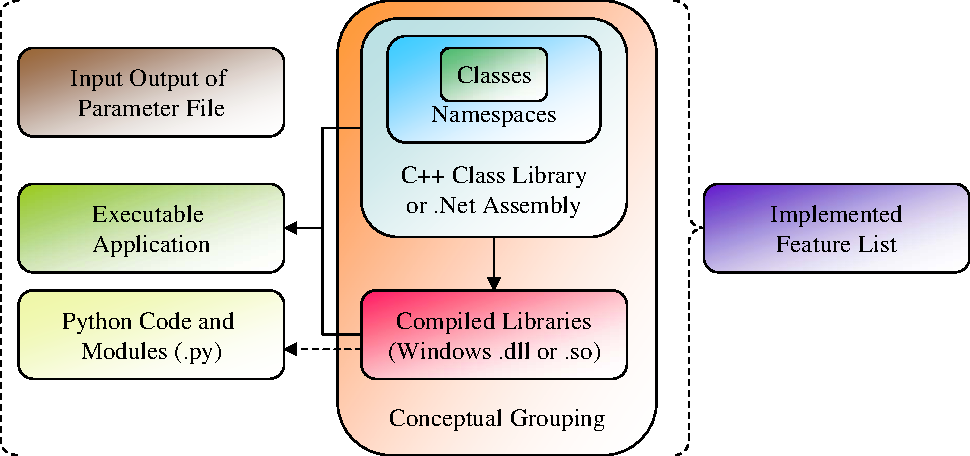
\includegraphics[width=0.8\textwidth]{03-Software/key/key.pdf}
\end{center}
\caption{The key for the conceptual software diagrams presented throughout the remainder of this chapter.}
\label{fig:software:conceptkey}
\end{figure}

We have already discussed the technical terms compilation, binary, executable and class. In addition to this a \emph{namespace} is simply a logical grouping of classes; two classes can share the same name as long as they reside within different \emph{namespaces}. Classes themselves can be distributed together in the form of a single library file as opposed to individual source code files. The subsequent compilation of such a compiled library results in a .dll (dynamic link library) file under Windows or a .so (shared object) file under Linux. Both of these essentially fulfil the same role of supplying a single logical code-base to multiple applications. Such compiled code can also be used by Python scripts, but requires non-trivial wrapper-code to import functionality. Class libraries for Microsoft's \dotnet\ also use the .dll filename extension and essentially perform the same role, but  work in a completely different way internally, meaning the two types are not compatible.


\clearpage
\section{PD}
\label{section:software:pd}

\pd\ is the name for the novel simulation framework developed, from the ground up, for this work in collaboration with Mike Tyka. 
\pd\ was developed with several principle objectives:

\begin{description} \isep

\item[Rapid and Easy Development] The central purpose of \pd\ is that it
should facilitate rapid algorithm and methodology development. 
\item[Coding Standards]
OOP principles should be used extensively throughout development.
Thus, all core concepts should be abstracted into a series of  highly-modular and intuitive base-classes. The number of base-classes should be minimised for simplicity, but remain representative of all common usage. Example class structures should be provided to guide novice programmers into the internal structure of \pd.
\item[User Interface]
Each component should be made completely
available to the user, through a powerful scripting interface, so that they can be logically recombined to form novel algorithms.

\item[Generality] \pd\ should provide a framework on which a very broad variety of applications in computational chemistry and biology can be built. It should presume as little as possible about the nature of the molecules to be simulated,
or indeed the nature of the simulation.
It is a core design decision that parameters are \emph{never} hard-coded. 

\item[Execution Efficiency] Many features in a simulation framework like  PD require high efficiency of simulation.
Importantly, these features \emph{must} all be implemented in a well established \emph{compiled} language.
As long as standard coding practices are used, this should allow both out-of-the-box efficiency and significant scope for optimisation.

\item[Platform Independence] It is important that \emph{only} ANSI/ISO standards are used for all code. 
Code must be both platform and compiler independent, which should make \pd\ intrinsically portable.

\end{description}



\subsection{Implementation}

Fundamentally, \pd\ is the conceptual unification of a high performance molecular mechanics library called \mmlib,  written predominantly in \CPP\ and exhibiting an automatically generated Python wrapper. Essentially, to use \pd\, the user simply writes a short
Python script which invokes functionality within \mmlib.

Python is intrinsically superior to the custom scripting engines used in other molecular mechanics frameworks like \amber\ and \charmm.
By contrast, applications written in
pure \CPP\ are capable of extremely high performance. The converse is not true. The performance of Python does not match that of \CPP. \CPP\ requires compilation and is therefore  intrinsically unsuitable as a scripting language. The solution to this conflict is a cross-language bridge, where code-division aids the fulfillment of the principle objectives. 

A potential disadvantage of defining \CPP:Python bridge-code
is increased developer overhead -- in fact this is a problem with the competing package \textsc{Ball}. In \pd\ this is completely avoided via automation of the wrapping process.
 The entire Python interface  is created automatically by an open source application called SWIG\cite{COMP:SWIG}.
Importantly, Python, SWIG and a host of efficient \CPP\ compilers are available for virtually all major operating systems and architectures.
Figure \ref{fig:software:pdusage} illustrates the interplay between the various framework elements. Primary usage is illustrated in the central grouping.

\begin{figure}[htbp]
\begin{center}
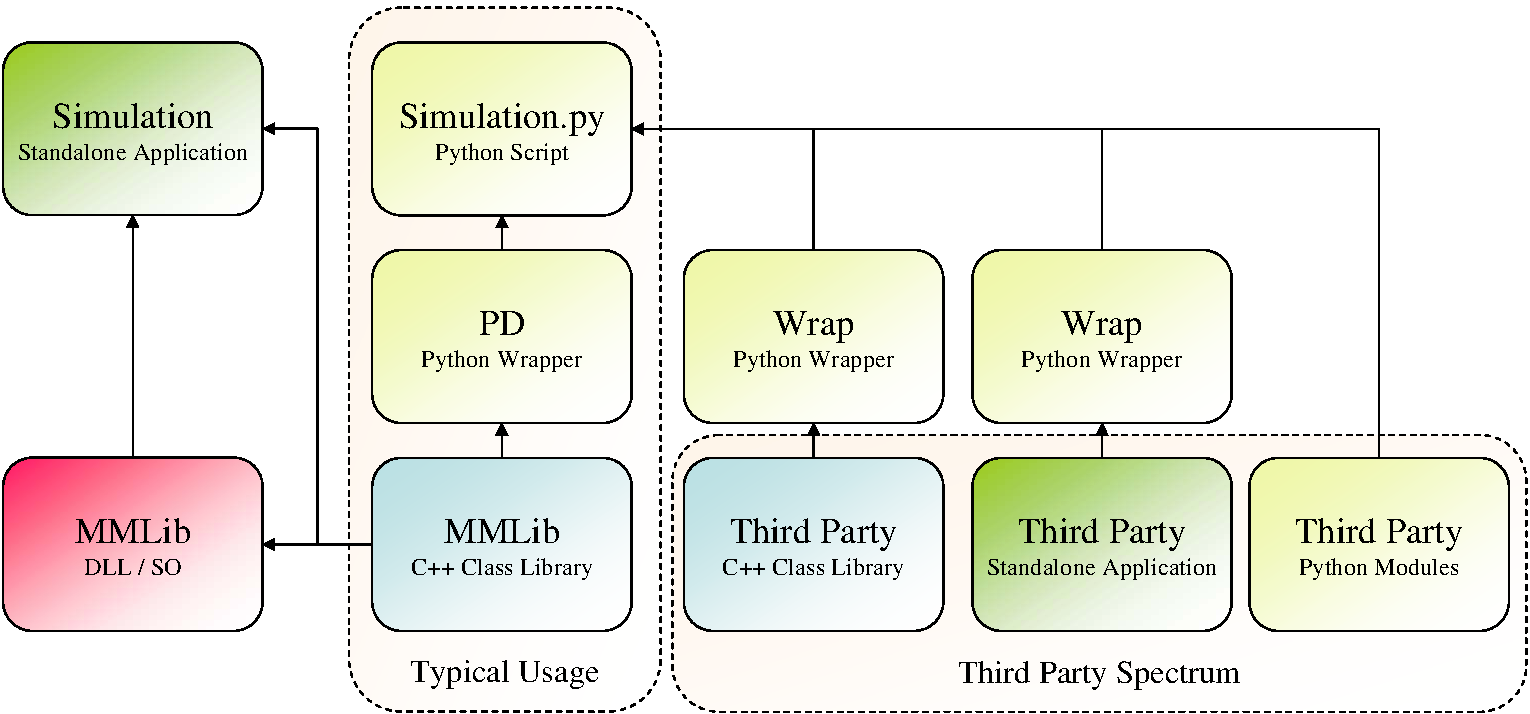
\includegraphics[width=0.95\textwidth]{./03-Software/pd/pd_framework.pdf}
\caption{Overall PD Structure and linking opportunities.}
\label{fig:software:pdusage}
\end{center}
\end{figure}




\subsubsection{The Core Library: MMLib}

The underlying framework of \pd\ is called \mmlib\ and coded in pure \mbox{\CPP.} \mmlib\ uses 
a \emph{minimal} series of abstract base classes to describe key ideas, which are are defined in section \ref{section:software:pd_code_overview}.
These base-classes are intuitive, well defined and interact in a modular manner. 
As most execution time is spent in the inner loops of forcefield calculations,
the use of this high-level abstraction comes with no measurable performance loss.
It is the view of the developers that this modular paradigm fits perfectly into the research environment.

Internally, \mmlib\ adopts standard OOP practice including industry standard design patterns,
pure ANSI \CPP\ and heavy use of the STL (the \CPP\ standard template library); which makes the code intrinsically
portable.
Although OOP principles are used throughout \pd, an important design choice was not to over-use
highly technical and non-intuitive code patterns. By keeping code inter-relationships
more simple there are a number of advantages. Primarily, over-complication
would go against the principle design ideals of \pd\ --  such practice
makes the code more difficult to understand and therefore makes algorithm
development \emph{less} rapid. Secondly, some language features (such as
virtual function calls), if used
inappropriately, can result in a significant performance penalty.




\subsubsection{The Python Interface}


Python is a fully-featured, well established, programming
language in its own right. A wealth of documentation and tutorials are available on the internet, meaning that the language is easy to learn for new programmers. All standard OOP constructs are available in addition
to the principle elements of procedural code such as arrays, conditional
statements and loops structures. These features are all far in excess of what you would expect to find built
into the input script parsers of the \amber\ and \charmm\ frameworks.
Python can also be used to completely replace traditional shell scripts in
terms of multiple job management. 

 
\pd\ takes integrated scripting to a new level. In addition to the rudimentary commands provided by other simulation engines, \pd\ provides all the basic building-blocks to formulate complex algorithms in abstract terms \emph{at the scripting level}. As the entire usable code-base is wrapped and exported automatically as a Python module, the latest features are \emph{implicitly} available to the Python user. Virtually every feature available by direct use of the underlying \CPP\ framework
is available through the Python interface.  By contrast to command-line flags, a Python interface vastly reduces the amount of manually written code necessary to expose available functionality. Not only is this incredibly powerful, but also extremely easy, freeing the programmer to worry less about code architecture and more about what he would like to accomplish. Use of the Python interface requires no recompilation --
it is often of benefit to be able to implement and tweak algorithms
in Python without the need to constantly recompile base-code.

In this
way
all the advantages of a custom scripting language are maintained as the
interface remains simple; however, as the user becomes more advanced, all
of the underlying functionality is available which allows complex algorithms can be created. For large developments, developers can add to the underlying \CPP\ framework
itself, whereby  their efforts will be \emph{implicitly} exported to the public Python interface for others to use.



 



 
 


\subsubsection{Alternative Code-base Access}

Typical usage of \pd\ is through the Python
interface, however, it is worth mentioning at this stage that although Python was chosen for
this work, SWIG is also capable of exporting for other common languages
such as TCL, Perl, PHP, and \CS\ (the \dotnet).

 
  
Figure \ref{fig:software:pdusage} also shows how the functionality of \mmlib\ can  be extended through
three potential Python-related paths. Python is sometimes described as having ``batteries included''. That is
to say, a great deal of third party functionality is available, very often free of charge, in what are called Python modules. These features can all be directly imported
into Python scripts. This includes modules for numeric analysis, SQL database interaction, networking, web services, graph
plotting and even OpenGL (3D Rendering). Secondly, entire third party applications could potentially be invoked via a Python-based manager. The subsequent output would be parsed and returned to the main script. Finally, just as with \mmlib, any other \CPP\
code library can also be wrapped using SWIG to make its functionality available.


The result of such modularity is that one could create, with minimal new code, an application which: loaded a series of  PDB identifiers from an\ SQL database; downloaded the files;  performed molecular dynamics simulations; all whilst plotting a graph of the energy. One such planned amalgamation
is an interface between \pd\ and \pymol; a very powerful and well-established molecular
graphics viewer, written mainly in Python, and free for academic use. This would give \pd\ very powerful graphical capabilities as well as greatly extending the simulation capabilities
of \pymol.

The Python interface is not the only way that functionality within \mmlib\ can be accessed --
two additional routes exist. The first is to statically link the \CPP\ class library
directly into a stand-alone simulation executable  which would perform a
specific function, but use the functionality within \mmlib. A second option
is the creation of a .dll file under
Windows or a .so file under Linux, which can be dynamically linked against other applications to give them bio-simulation capabilities.



\subsection{A Real-World Example}


The best way to illustrate just how well the small number of base classes
that \pd\ uses are able to very concisely describe typical molecular simulations is to show an example.
Each class has a clear purpose and each links into the next, ultimately  defining the  simulation.
Each of the code-boxes below represents a  section of the same python script.
Each section is discussed in turn. 

\lstset{language=Python} % For all listings in this enumerations
\begin{enumerate} \isep

\item The first thing one needs to do in any python script is to import all
required modules. As we are only defining  a simulation, all that is needed is the \pd\ module.

\begin{lstlisting} 
from pd import *                   # Load the pd module!
\end{lstlisting}

\item Next  \pd\ format forcefield parameters are loaded. These are contained within a parameter file that
describes both molecular topology and parameters for various
energetic forcefield components; previously described in section \ref{section:protmodel:energy_functions}. The topology is essentially
a list of named molecules, their atoms and associated properties.
\begin{lstlisting}
ffps = FFParamSet()
ffps.readlib("amber03aa.ff")       # Load the standard AMBER ff03 parameters
\end{lstlisting}

\item The forcefield parameters are now passed to a newly created \textsl{System} class which can represent any molecular system. Internally, it contains a
number of hierarchical dynamic arrays which contain \textsl{Molecules}  and functions required for their manipulation. In the example below we
use PDB\_In which \emph{derives} from System, augmenting it with the abilities to
read molecules from PDB files.

\begin{lstlisting}
sim = PDB_In( ffps, "myprotein.pdb" ) # PDB_In is a type of System
sim.load()                            # Load everything from the PDB file
\end{lstlisting}

\item The primary purpose of the \textsl{System} is to represent molecules in a hierarchical
manner, which makes manipulation of the underlying system more simple, for
example it is very easy to duplicate molecules. A hierarchical representation
however does not lend itself to efficient computation -- for this a more classical
linear array of atoms is required. This is provided by the class \textsl{WorkSpace},
which is generated from either the entire system or a defined sub-section which
requires efficient simulation. Such a sub-section could be a surface loop and
surrounding protein core residues.
Each of the appropriate atoms is then replicated within the \textsl{WorkSpace}.

\begin{lstlisting}
wspace = WorkSpace( sim )
wspace.info()                     # Prints a small block of info about the contents    
\end{lstlisting}

\item A \textsl{Forcefield} is now required to describe the energetics of the system.
In the example below we add the standard \amberff\ bonded forcefield and
a simple non-bonded forcefield with VDW\ interactions and vacuum electrostatics. \pd\ also implements many other more sophisticated forcefield components beyond the scope of this discussion.  

\begin{lstlisting}
ff = Forcefield(wspace)           # Initialise a Forcefield container with a link to 
                                  # a WorkSpace instance
bonded = BondedForcefield()       # Create the bonded forcefield component
nonbonded = NonBondedForcefield() # Create the non-bonded forcefield component

ff.add( bonded )                  # Add both to the parent container
ff.add{ nonbonded )               # 

ff.info()                         # Print the energetics of the pre-simulation system
\end{lstlisting}

\item In this particular example, the user wishes to perform a 1,000 step
conjugate gradient energy minimisation. We simply create an instance
of the \textsl{Minimisation} class.

\begin{lstlisting}
min = Minimisation( ff )          # Tell the minimisation what its forcefield is
min.Steps = 1000                  # Change the number of steps from the default to 1000
min.UpdateScr = 10                # We choose to update the screen every 10 steps
\end{lstlisting}

\item We may also decide that we wish to monitor changes in a given set of system properties, such as structural deviation from the starting conformation. As such,
one or more \textsl{Monitors} can be added to the simulation. \textsl{Monitors} can include
those for energy terms, RMSD values and other geometric quantities. After such
monitors have collected data, multiple statistical quantities can be requested.

\begin{lstlisting}
mon = CRMSMonitor( wspace )       # Create a new cRMS Monitor
min.addMonitor( mon )             # Add it to the simulations monitor container
\end{lstlisting}

\item Finally, we execute the simulation. The requested 1,000 steps of energy
minimisation are performed and  the screen is updated with energetic
information. 

\begin{lstlisting}
min.run()                         # Execute the simulation
\end{lstlisting}

\item Once complete, we can ask the Forcefield to print an energy
report and the monitors to show their measurements. 

\begin{lstlisting}
ff.info()                         # Print the energetics of the post-simulation system

mon.printHeader()                 # Print a nicely fomatted title
mon.printCurData()                # Print the curent cRMS
mon.printHistogram(0.1)           # Print a histogram of the recorded data
\end{lstlisting}

\end{enumerate}

So in only 23 code lines, we have represented and executed a complex energy minimisation,
reporting only the data that was relevant to the user. Even though this
script is short, it embodies almost every major aspect of \pd\ and illustrates
the use of 7 of the 10 primary base-classes.

The defining feature of the \pd\ Python interface is that it is clear, intuitive and
human readable; especially in comparison to
the equivalent \charmm\ script (listing \ref{listing:software:charmm}, discussed in section \ref{section:software:prob4progflow}) which doesn't have the same extensibility or
encapsulated data monitoring capabilities. Legacy custom scripting languages  also tend to
use rather cryptic commands such as ``hbuild sele all end'' which make incomplete sense without complementary well-written  documentation.
It is, therefore, the view of the \pd\ developers that \pd\ has features which are unprecedented in comparison to all older frameworks. This   makes \pd\ \  clearly superior in terms of user interaction.

\subsection{Fundamental Class Overview}
\label{section:software:pd_code_overview}

In the following section, a \emph{brief} overview of the defining elements
of \mmlib\ will be presented along with simplified typical usage. Figure
\ref{fig:software:pdclasses} shows the primary class relationships within
\pd\  (although there are others) which will be described below.

\begin{figure}[htpb]
\begin{center}
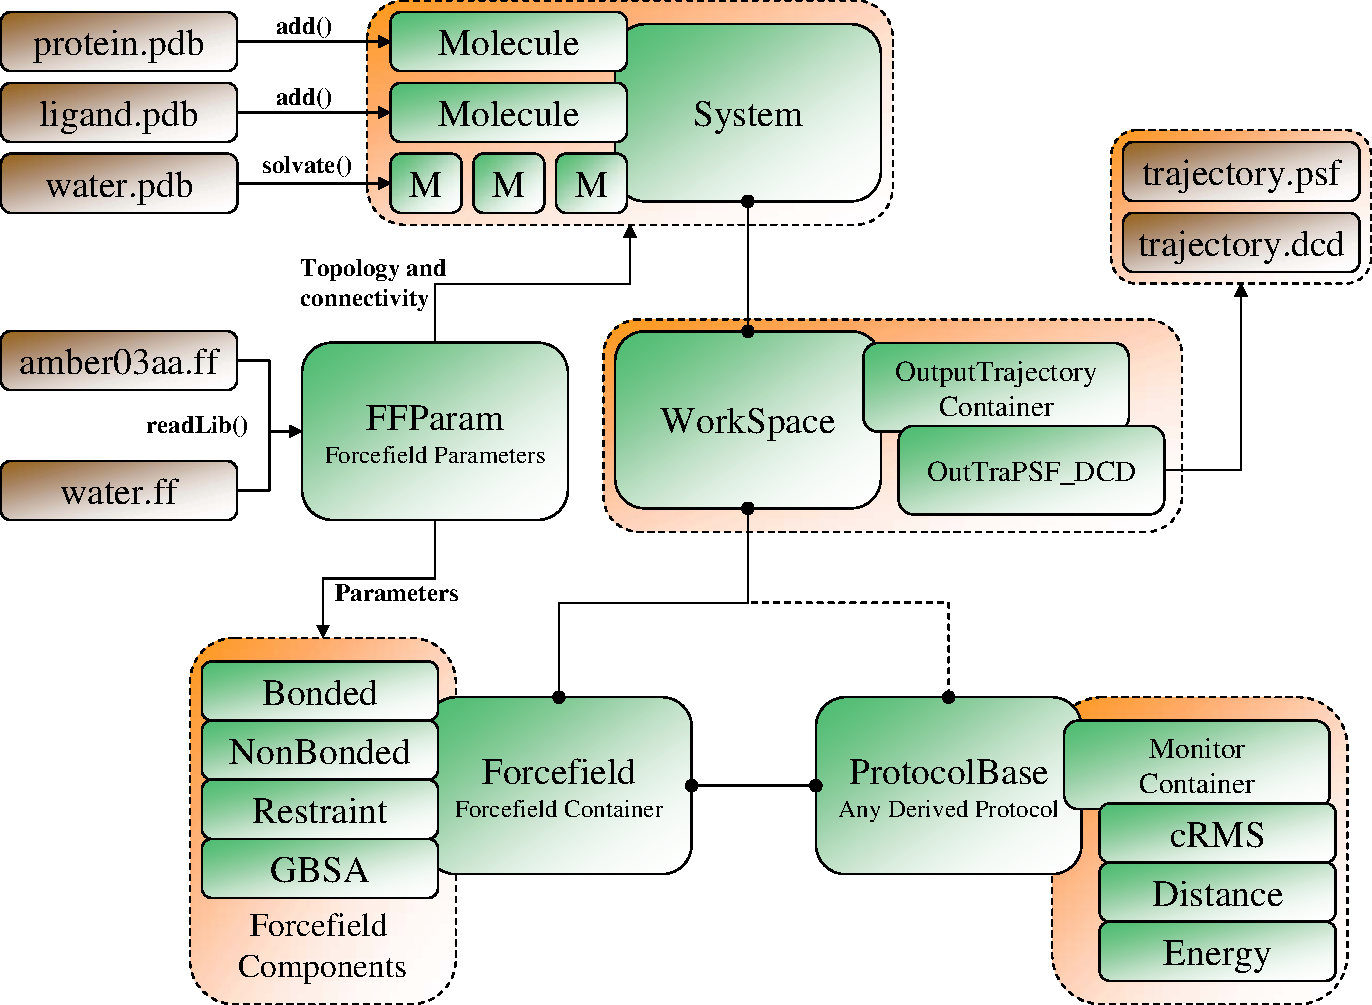
\includegraphics[width=0.95\textwidth]{03-Software/pd/class_Relationship.pdf}
\caption[\pd\ base-class relationships]{\pd\ base-class relationships. System is used to manipulate the pre-simulation molecular state. The central triad of the \textsl{WorkSpace}, Forcefield and \textsl{ProtocolBase} are used to embody the simulation itself. The various leaf elements and files are used to either import or export information.}
\label{fig:software:pdclasses}
\end{center}
\end{figure}

\subsubsection{A Consistent Model}

To reduce the learning-curve for both the use and development of \pd, it is important to maintain consistency
between different aspects of the framework. 
One such common theme throughout \pd\ is an abstract base class, with complementary
collection class. This statement might seem complex, but is actually quite
simple and is defined below.

In section \ref{section:software:inheritance} inheritance and its advantages were briefly discussed, along with a definition for the term base-class.
An \emph{abstract} base class is essentially the same, but does not implement one
or more of its member functions. You can never create an object from an abstract base class, you can only derive form it. Classes which derive from abstract base classes
must implement the missing functions, or they remain abstract themselves.

This concept makes sense in \pd: An excellent example for the use of an abstract base class in \pd\ is \textsl{ForcefieldBase}, which embodies the concept
of a forcefield component. Every derived forcefield component \emph{must} implement
the function calcEnergies(), which of course cannot be done until one knows
exactly what the component does. Each forcefield component does, however, share a good
deal of common functionality, including the need for addition into a common forcefield
container to perform its function. Another perspective of this is that, once a programmer has derived from \textsl{ForcefieldBase} and implemented all the required functions, his class is guaranteed to fit into the framework and can therefore
be used with all other available functionality.
 
Secondly, the \textsl{Forcefield} class \emph{is} simultaneously a
collection class and a type of \textsl{ForcefieldBase}. The role of the \textsl{Forcefield} collection is to hold other forcefield components. When the  \mbox{calcEnergies()}
function of the collection is called, it simply sums the return value of the \mbox{calcEnergies()} call
for each of its children. As such, the Forcefield container itself may be added
to a parent Forcefield container and thus forcefields can be \emph{managed as groups}, adding hierarchical flexibility to the framework.

The paradigm
of an abstract
base class and a container class which itself derives from that base is used again and again for each of \textsl{MoveBase},
\textsl{FilterBase}, \textsl{MonitorBase} and \textsl{OutputTrajectory}.

\subsubsection{FFParamSet}

\textsl{FFParamSet} is a \emph{run-time} database of chemical information and complementary
simulation parameters. Following creation of the class instance, data is imported form one or more \pd\ format ``.ff'' files, which are inspired by the
\charmm\ format, but borrow some superior elements from other formats. Code to parse the\  \charmm\ forcefield
format itself is, at the time of writing, undergoing further development. This additional parser implicitly extends the available forcefield sources
for \textsl{FFParam}, as many varied forcefields are already publicly available in
\charmm\ format, such as the \textsc{Opls} \forcefield. 

Once data is loaded, definitions are present for the chemical make-up of
polymers, residues and atoms. These data include atomic types, connectivity, radii, force constants, torsional parameters, amongst specific parameters
for individual specialised forcefield components. Robust data parsing is one of the most code-intensive activities within a given framework.  
As all simulation parameters can be loaded and stored via this class, which also facilitates subsequent structured
data access, no other components ever need to parse their parameters from separate files.
This greatly reduces the amount of IO code required and therefore reduces
both code complexity and maintenance requirements.

\subsubsection{System}

A \textsl{System} class is a container for the class \textsl{Molecule} and contains functions
concerned with the forcefield-independent geometric manipulation and duplication
of these
molecules. \textsl{Molecule}, in turn, owns both atom coordinates and properties.
Importantly, \textsl{System} is a hierarchical container representing intuitive relationships between chemical entities. All connectivity information is supplied by the \textsl{FFParamSet} class instance which is passed to \textsl{System} in its constructor. 


\subsubsection{\textbf{FileInBase}}

\textsl{FileInBase} is an abstract base class which derives from system, representing a file format which
contains molecular information, such as the PDB format. As an \textsl{FileInBase} \emph{is a} \textsl{System}, it merely adds functions that can import molecules from a file, but is essentially used as a standard \textsl{System} instance.

\subsubsection{WorkSpace}

The \textsl{WorkSpace} is always created from a \textsl{System} and is intended to hold the current simulation state. Potentially, multiple \textsl{WorkSpaces} can be created for a given \textsl{System}, in a one-to-many relationship. A practical example of this could be in protein surface remodelling where
each loop could be treated as a separate \textsl{WorkSpace} with minimal surrounding
atoms.

Each atom has properties
like Cartesian position, force and velocity, which may or may not be used
in use for a given simulation. Importantly, it is the classes that derive from \textsl{ForcefieldBase} and \textsl{ProtcolBase} which are allowed to modify these properties. The \textsl{WorkSpace} retains an internal link to its parent \textsl{System}, so that \textsl{System} properties can be updated following simulation. 

The \emph{critical} aspect of the \textsl{WorkSpace} is its internal linear atom array,
which is the primary distinction from the \textsl{System} class. This
concept allows in-code logic optimisations, but also critically benefits
the highly-optimised memory pipe-lines of modern computing architectures. Briefly,
memory is brought to the processor in \emph{pages}, which are defined as
short sections of contiguous memory. If memory is requested outside this range, then the processor must wait for it to be delivered, drastically reducing performance. By ensuring that the underlying memory is contiguous -- \ie\ the linear atom array -- the computers paging operations become more
efficient and thus execution times are reduced. 

\textsl{WorkSpace} supplies a number of additional plug-in components, each of which
provides easy access to pre-defined information regarding the nature of the
underlying molecular system. These include
the \textsl{BondOrder} array, which defines the order of the connectivity between
atoms in the \textsl{WorkSpace}; the \textsl{NeighbourList} which stores information as to
which atoms are proximal to one another; the rotatable bond array,
\textsl{RotBond},
which dictates which bonds can be rotated within a torsional representation;
and finally the \textsl{OutTra} container which can hold one or more output trajectory objects of any defined format.
\textsl{WorkSpace} also supplies a vast variety of functions to alter the Cartesian
and torsional states of the molecules that it contains.

\subsubsection{ForcefieldBase}

Each \textsl{ForcefieldBase}-derived class represents a forcefield component. When it makes sense
to do so, for example if it is more computationally efficient, some related
components are calculated together. An  example of this is the bonded forcefield components described in section \ref{section:protmodel:bondedterms} and shown as a single unit in figure \ref{fig:software:pdclasses}.

Each derived class 
is ultimately going to implement  two key functions; \mbox{calcEnergies()} and, if it is capable of supplying first derivatives, also \mbox{calcForces()}.
All parameters for execution are supplied by the \textsl{FFParamSet} instance passed
to the component when it is created. Following execution of these statements, the variables holding energetic terms within the \textsl{WorkSpace}
are incremented and the forces summed onto each atom's current force. It is
the Forcefield container class which is responsible for invoking the calcEnergies()
or calcForces() of each of its subordinate \textsl{ForcefieldBases} \emph{when directed} by the currently active \textsl{ProtocolBase}. 
 



A useful feature is that individual forcefield components can be activated
or deactivated as the user sees fit during execution. Additional \forcefield\ components
can also be added at any time as the user sees fit. This gives the user full
control over the progression of the simulation. Individual components can
also be made passive, whereby they do not contribute to the energy of the
system. This can be useful if one wants to monitor what the value of a given term would be, whilst not wanting to influence the active \textsl{ProtocolBase}. 

It was discussed in section \ref{section:protmodel:comparativemodellingarchetypes},
that the most successful comparative modelling methods are those which can include a variety of experimentally and statistically derived restraints. The modularity of the forcefield component paradigm used in \pd\ lends itself
perfectly to this, as forcefield components can be dynamically added for any imaginable
restraint or constraint. 

\subsubsection{ProtocolBase}

Classes derived from \textsl{ProtocolBase} are responsible for moving atoms in the
\textsl{WorkSpace} in response to the energies and forces described
by the \textsl{Forcefield}. As such, the \textsl{ProtocolBase} is essentially at the core
of the entire simulation. The simulation behaviour is provided by the implementation
of the function run\_core(), which makes all the decisions.
Each protocol owns a \textsl{MonitorBase} container which monitors the
result of its activities.

The basic set of implemented protocols is essentially most of the conformational search algorithms
defined in section \ref{section:protmodel:conformational_search}, along with other
techniques such as energy minimisation and higher-level protocols for loop
building and protein docking. These basic protocols do not have to act alone, but can be nested, partnered and extended by the user to
create novel kinds of simulation. Importantly, it is the common interface\ which allows this to work, as by definition all protocols must implement run\_core().
Good examples of how this can be done
are described later in section \ref{section:software:extendpd}.

 
\subsubsection{MonitorBase}

The idea of a Monitor is a very low-level abstract concept. As such, classes
which derive from \textsl{MonitorBase} really can monitor any quantity.
Each derived class simply implements the function setcurdata(), which is required
to set
a single member variable to the value of the measurement. The remainder of the functionality, such as producing histograms, calculating statistical properties and  printing
data is all provided by the base class. Creation of a new Monitor is trivial
as only one function need be implemented.

 
The measurements themselves are directed by the parent \mbox{\textsl{ProtocolBase}},
which informs its \textsl{MonitorContainer} to sample at a defined interval throughout
the simulation. As per the \pd-standard paradigm, the container is then responsible
for calling the measure() function of its children, causing them in turn
to call their own setcurdata(). This process results in a neat and intuitive
division of labour and a clear order of power.

\subsubsection{MoveBase}

Classes which derive from \textsl{MoveBase} are useful to a more limited set of \textsl{ProtocolBase}
classes which utilise discrete moves within their conformational search.
An example of such a class is  \textsl{MonteCarlo}. This Protocol owns a
\textsl{MoveBase} container (the paradigm returns) and calls each contained move in turn during the course of the simulation. Such moves could include Cartesian perturbations, torsional perturbations and rotamer assignments, as well as other more specific kinds. The exact composition is always defined by the users requirements.

\subsubsection{PickBase}

Some \textsl{ProtocolBases} use atom pickers, which derive all from \textsl{PickBase}.
These classes simply implement a single function which takes a reference
to a given atom and returns true or false as to wether that atom is within its
selection. Figure \ref{figure:software:pickingvenn} illustrates how basic pickers can be easily combined. As the protocol \textsl{PickedMinimisation} has been
implemented, this selection of pickers could be used, for example, to resolve \sidechain\ steric clashes in the N-terminal section of a protein model, without disturbing the remainder of the model. 

\begin{figure}[htpb]
\begin{center}
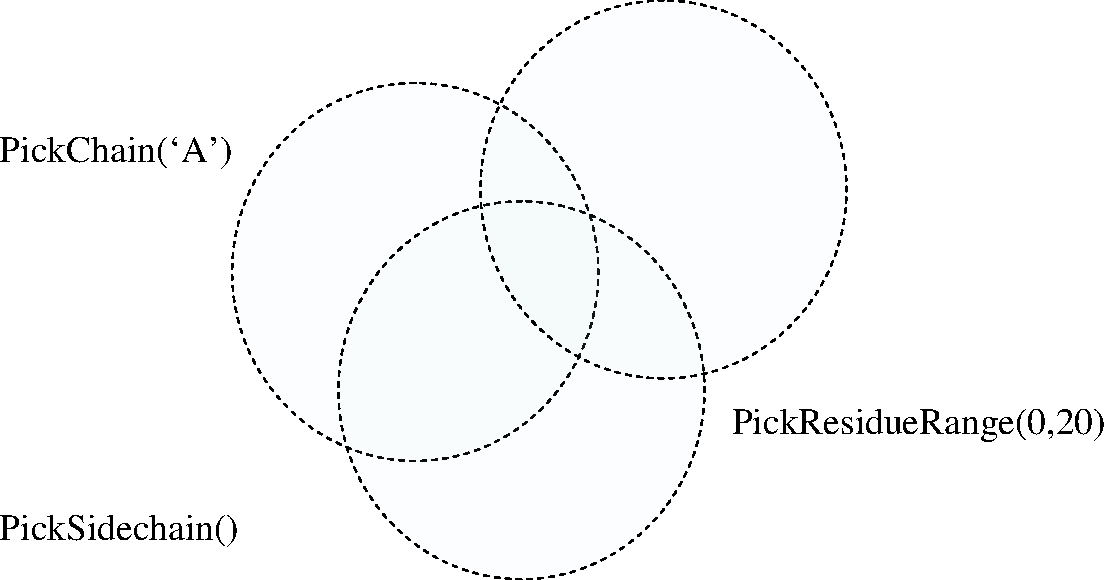
\includegraphics[width=0.7\textwidth]{03-Software/pd/picking.pdf}
\end{center}
\caption[Atom Picking in \pd]{A venn diagram showing how 3 basic pickers can
be combined to select only the \sidechain\ atoms of the 20 N-terminal residues of chain A.}
\label{figure:software:pickingvenn}
\end{figure}


\subsubsection{FilterBase}

\textsl{FilterBase} is intended as a mechanism to improve the sampling efficiency
of a given \textsl{ProtocolBase}. In some cases, especially when
large conformational change \textsl{MoveBases} are utilised, non-sensical conformations
can be generated during a simulation. As the main forcefield calculations are comparatively expensive,
it can be helpful to pre-screen conformations, only performing the  full evaluation on those which pass all filters.
Good examples of such filters are hard-sphere steric filters in MC simulations,
a bond-length filter, or a filter that tests to see if the \Omg\ peptide-group
torsion is within a given tolerance of 0\degree\ or 180\degree.  

\subsubsection{OutputTrajectory}

Output trajectories capture snapshots of a given workspace as directed by
the active \textsl{ProtocolBase}. As usual, these classes derive from a single class called \textsl{OutTraBase}, 
which embodies the basic properties of a trajectory such as the file-stem. It has already been stated that the 
\textsl{WorkSpace} owns an \textsl{OutTraContainer} object, which is commonly called by instances of \textsl{ProtocolBase}.  


\subsection{Examples of Extending PD Functionality}
\label{section:software:extendpd}

The aim of the following section is to describe how \pd\ can be extended
both by the user and the developer and how the supplied class framework acts to supply maximum flexibility in this endeavour. By allowing extension
and reuse of existing elements, development time can be reduced. 



\subsubsection{Extension Using Python Code}

\pd\ can be extended at the user interface itself, via the nesting of existing protocols. Unlike other frameworks, this does not require a single line
of new \CPP\ code to be written. 

Take for example the \textsl{MonteCarlo} protocol, which has a vast number
of uses\cite{SIMULATION:MC}. In its simplest form, the \textsl{MonteCarlo}
algorithm makes conformational changes which are then evaluated by ``the evaluator''. The conformational changes are supplied by the \textsl{MoveSet,} which contains multiple
component perturbations added by the user. By default
the protocol functions by the standard Metropolis criterion of acceptance\cite{SIMULATION:Metropolis};
rejected structures are restored to their previous valid state. In the simple case,
the evaluator is a \textsl{ProtocolBase} which does nothing except trigger a \textsl{Forcefield} energy calculation.


The following examples assume that we have already configured a \textsl{FFParamSet},
\textsl{System}, \textsl{WorkSpace} and \textsl{Forcefield}; ignoring both
\textsl{Monitors} and \textsl{Filters,} although of course these could easily be added. In this example, we exploit the MC algorithm
to pack \sidechains.



\lstset{language=python}
\begin{lstlisting}[float=h] 
# Add together an appropriate selection of MoveBases
moveset = MoveSet(wspace)                     # An empty container...
moveset.add( SidechainRotamerLibMove( ... ) ) # add a low probability move
moveset.add( SidechainTorsionalMove( ... ) )  # than a high probability move

# Configure the simplest evaluator, a ProtocolBase 
# which triggers a forcefield calculation
evaluator = Energy(ff) 

# Create a MonteCarlo protocol instance
mc = MonteCarlo( evaluator, moveset )   # Giving it some moves and a Protocol by which to evaluate
mc.Steps = 200                          # Perform 200 MonteCarlo iterations
mc.TargetTemp = Temp(300)               # Simulate at a constant temperature of 300K

mc.run()                                # Lets go!
\end{lstlisting}

Now that we have created an underlying system, the user can begin to experiment
with many different options. Firstly, we can change the temperature profile
from static to a linear decay. 

\lstset{language=python}
\begin{lstlisting}
# Create a MonteCarlo protocol instance
mc = MonteCarlo( evaluator, moveset )   # Giving it some moves and a Protocol by which to evaluate
mc.Steps = 200                          # Perform 200 MonteCarlo iterations
mc.TargetTemp = TempLinear(300,10)      # Simulate at a constant temperature of 300K

mc.run()                                # Lets go!
\end{lstlisting}

The linear temperature regulator automatically scales the temperature factor
from 300K to 10K over the course of the 200 steps. Other temperature profiles
are implemented such as exponential decay. Thus, with a single code line change, we have now implemented Metropolis MC with simulated annealing. 

A second potential change is of the evaluator, which is invoked prior to the
decision as to wether a structure should be accepted. If large conformational
moves are used, an obvious choice is an energy minimisation. 

\lstset{language=python}
\begin{lstlisting}
evaluator = Minimisation(ff)            # Configure a minimisation

# Create a MonteCarlo protocol instance
mc = MonteCarlo( evaluator, moveset )   # The passed evaluator is now different...
mc.Steps = 200                          
mc.TargetTemp = Temp(300)  

mc.run()                                # Lets go!
\end{lstlisting}

Again, with a single code change, we now have a Protocol with completely different
properties -- we have implemented Metropolis Monte Carlo with minimisation\cite{SIMULATION:MCM}.
A similar nested protocol change would be to use Molecular Dynamics with
a small number of steps at the
evaluator, creating Hybrid Monte Carlo\cite{SIMULATION:HybridMC} -- again this
only requires minor changes to the code, but creates a completely different algorithm. 


Finally, we have mentioned that Python can be used as a replacement for shell
scripts for managing multiple complementary simulations. Both replica exchange
molecular dynamics and replica-exchange Monte Carlo, REMD\cite{SIMULATION:REMD} and REMC\cite{SIMULATION:REMC} respectively,
require the coordination and exchange of parallel simulations. For these, the management
and exchange logic would need to be implemented in Python; essentially the
algorithm controlling the
temperature and coordinate exchange. 
This should be done in a generic manner; REMD and REMC actually share a majority of the same Python code and like the MC examples the only real difference
is the choice of evaluator. This single simulation script, as opposed to using
shell scripts, puts all code in one place, making it easier to maintain and more powerful due to the specific
advantages of Python.




\subsubsection{Extending Using New C++ Code}

Although the recombination of features via the Python interface is incredibly useful,
completely new features and algorithms will always require new \CPP\ code. It is hoped that the comprehensive nature of the \pd s base classes will mean that no additional bases are required. Inheritance, described in section \ref{section:software:inheritance},
is therefore an important mechanism. 
 
 
 
 As discussed in section \ref{section:protmodel:stun}, STUN\cite{SIMULATION:STUN}
 is a method which shares a significant amount of functionality with the
 standard MC algorithm, differing only by its acceptance function. Because
of this, there is little point in creating new code for anything apart from the acceptance function itself. By \emph{deriving} from \textsl{MonteCarlo}, \textsl{STUN} gains all of its functionality and is allowed to replace or \emph{overload} the accept() function call with new logic, reusing all other
code.

An advanced topic that is used throughout \pd\ is \emph{multiple} inheritance.
Rather than deriving from a single base class, in some circumstances, it can be appropriate to derive from two or more. 
An example of where this could be useful involves a class which derived both from \textsl{MonitorBase} and \textsl{NormalMode} and adds a small amount of stitching-code. 
This hybridisation, via multiple inheritance, effectively defines a crude entropy monitor for use during the course of a given simulation.  


\subsection{The List of Implemented Features}

At the time
of writing, a large number of features have already been implemented in \pd\  and a significant amount of functionality is planned for imminent
implementation.
The features that are used in this thesis are only a subset of the available scope of \pd. 

\begin {itemize} \isep
\item{Forcefield Components}

    \begin {itemize} \isep
     \item\textit{Bonded:}    Harmonic bonds, angles, fourier harmonic torsions and impropers. 
     \item\textit{Non-Bonded:} Lennard-Jones, \vdw, simple electrostatics. Energy and force switching functions.
     \item\textit{Spaces:} Infinite vacuum, periodic boundary conditions (orthogonal)    
     \item\textit{Solvation:} Distance-dependent dielectric constant\cite{FORCEFIELD:DistDepDi}, solvent accessible surface area (SASA) based solvation including both Eisenberg et al.\cite{FORCEFIELD:SASA:Eisenberg} and Ooi et al.\citep{FORCEFIELD:SASA:Ooi}, POPS\ algorithm for SASA by pairwise distance approximation\cite{FORCEFIELD:POPS}, generalised Born / surface area (GB/SA) \citep{COMPCHEM:Still90,FORCEFIELD:Qui1997,FORCEFIELD:Zhang2003}.      
     \item\textit{Knowledge Based:} Residue:residue interaction-matrix.     
     \item\textit{Restraints:} Harmonic, Cartesian distance and torsional restraints. Miscellaneous custom forces.
     \item\textit{Other:} G\={o} type forcefield, soft-sphere VDW Forcefield
    \end {itemize}

\item{Forcefield implementations:}
        \begin {itemize} \isep
           \item\textit{\amber}:  ff94 \cite{FORCEFIELD:AMBER:94}, ff99\cite{FORCEFIELD:AMBER:99}, ff03\cite{FORCEFIELD:AMBER:03}   
           \item\textit{\charmm}\cite{FORCEFIELD:CHARMM}: \charmm-19, \charmm-22
           \item\textit{\opls}:   \opls/aa\cite{COMPCHEM:OPLS:C}
           \item\textit{Other}:   \textsc{Bude}\cite{THESIS:SOPHIE}, \raft\cite{COMPCHEM:Gib2001}
        \end {itemize}  
        
\item{Protocols \& Algorithms:}         
        \begin {itemize} \isep
           \item\textit{Gradient based Minimisation}: Steepest Descent, Conjugate Gradients and Torsional\cite{THESIS:BREWER}.               
           \item\textit{Monte Carlo}\cite{SIMULATION:Metropolis}: Monte Carlo with minimisation (MCM) \cite{SIMULATION:MCM} 
           \item\textit{Structural Perturbations}: A large variety including rotamer libraries\cite{COMPCHEM:RICHARDSON} and
          fragment insertions.  
          \item\textit{Comparative modelling}: Sequence alignment, threading, missing atom rebuild, \sidechain\ packing and loop modelling.          \item\textit{Conformational space annealing}\cite{SIMULATION:CSA}
          \item\textit{Molecular Dynamics}: Beeman \cite{SIMULATION:MD:Beeman}, Verlet and velocity Verlet integrators, Andersen \cite{SIMULATION:MD:Andersen} and Berendsen thermostats \cite{SIMULATION:MD:Berendsen}. (NVE, NVT and NPT).           \item Langevin Dynamics \cite{SIMULATION:Langevin}
           \item \textit{Replica Exchange Dynamics}  (REMD) \cite{SIMULATION:REMD}
           \item Numerical second derivate matrix (Hessian) calculation and normal mode analysis
           \item Quasi harmonic analysis \cite{SIMULATION:QuasiHarmonic,SIMULATION:QuasiHarmonic:B}
           \item\textit{Free-energy calculations}:  Free energy perturbation (FEP) \cite{SIMULATION:Zwanzig54}, thermodynamic integration \cite{SIMULATION:Kirkwood35,SIMULATION:Beveridge89}, umbrella sampling \cite{SIMULATION:UmbrellaSampling} and confinement methods \cite{THESIS:TYKA:PAPER06,THESIS:TYKA}
           \item Peptide \& protein docking\cite{THESIS:SOPHIE,THESIS:CRISP}
        \end {itemize}  
                        
\item{Monitors:}
        \begin{itemize} \isep               
          \item\textit{Structural deviation}: Cartesian and torsional RMSD measures
          \item Inter-atomic distances
          \item Native contacts
          \item Radius of gyration
          \item Energy components
        \end{itemize} 
        
\item{Rotamer Libraries:}
        \begin{itemize} \isep               
          \item Shetty\cite{NATIVE:Shetty2003}
          \item Rickardson\cite{COMPCHEM:RICHARDSON}
          \item Dunbrack\cite{NATIVE:Dunbrack2002} (Backbone dependent and independent)
        \end{itemize}
        
\item{Rotamer Packing:} 
        \begin{itemize} \isep               
          \item \textsc{Scwrl}\cite{METHOD:SCWRL_1,METHOD:SCWRL_2}
        \end{itemize}
                  
\item{Major file and trajectory formats:}
        \begin{itemize} \isep               
         \item PDB
         \item TRA (Bristol Trajectory Format)
         \item DCD \& PSF (used by \charmm\ and \namd)
         \item TRR \& XTC (Compressed trajectory format used by \gromacs)
        \end {itemize} 

\end {itemize} 





\subsection{Accessory Features and Advantages}

\pd\ as a framework comes with other implemented management features and benefits over
some other frameworks, including:

\begin{description} \isep
\item[Automatic Documentation] It is often said that the most up-to-date documentation is always the code itself. \pd\ uses the Doxygen code documentation system, whereby comments embedded within the code are parsed and corresponding documentation automatically generated. Output can be produced in many popular formats such as HTML and PDF. An excellent feature is that code-relationship diagrams are generated automatically and have hyperlinks allowing direct exploration of  code and associated comments. Currently such documentation is generated automatically on a nightly basis on the \pd\ web-server.
\item[Version Control] \pd\ is archived using Subversion -- an open source and well-supported version control system. As such, there is only ever one official version of \pd, whereby all developers work on their snapshot of the primary version and regularly commit updates. This greatly simplifies collaboration and implicitly documents all code changes and who made them.
\end{description}


\subsection{Benchmarks}

\pd\ is still in rigorous development and so far 
little time has been spent directly on code optimisation. Some
preliminary benchmarks have been made to test the feasibility of the underlying code-model.
Three separate benchmarks have been made against other respected packages, including \charmm\cite{FORCEFIELD:CHARMM}, Tinker\cite{COMPCHEM:TINKER}, NAMD\cite{COMPCHEM:NAMD} and Amber v8 (Sander)\cite{FORCEFIELD:AMBER}, and are shown in figure \ref{fig:software:pdbench}.

\begin{figure}[htbp]
\begin{center}
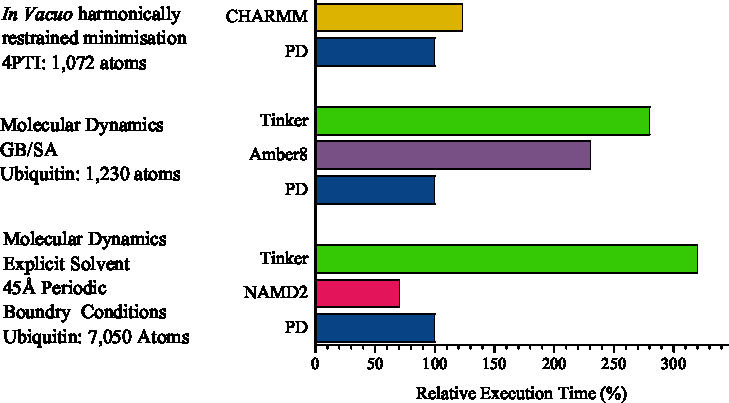
\includegraphics[width=0.9\textwidth]{03-Software/pd/benchmark.pdf}
\caption[Initial \pd\ Benchmarks]{Initial \pd\ Benchmarks. The MD data is reproduced courtesy of M. Tyka.}
\label{fig:software:pdbench}
\end{center}
\end{figure}

For a basic restrained minimisation protocol, \pd\ is shown to outperform \charmm\ version 3.0 (beta 2), reducing execution time by around 20\%. 
\pd\ also outperforms the Sander version of \amber\footnote{It should be noted that the Sander module
of \amber-8 is reported to be slightly slower than that of the newest GB/SA implementation in
\amber-9 (pmemd), which was unavailable within our group at the time the
benchmarks were computed. Thus, the performance of  \pd\ is most likely comparable to the latest \amber\ code.} and is competitive in execution time with \namd; each of which are respected applications in the
simulation community. \pd\ performs significantly better than \textsc{Tinker} on both MD examples, reflecting \textsc{Tinker}s lack of emphasis on raw performance.
The increased performance of \pd\ over \amber\ is attributed to code sections within \mmlib\ which have received most optimisation, especially
the GB/SA component. \namd\ is one of the most respected packages in terms of performance, having been developed by a large team for some time. It is therefore unsurprising that it outperforms \pd\ at the current time, although the relatively small difference is encouraging. It should
be noted that the periodic boundary code in \pd\ is still in developmental
form and lacks some of the most recent algorithmic enhancements that will
be present in \namd.


 \subsection{Concluding Remarks}


The main purpose of \pd\  is
as a highly flexible simulation framework. It is hoped that this overview has demonstrated that \pd\ achieves greater flexibility for the user than most competitors and where equal, already achieves 
higher performance. In addition, there is still significant scope for further optimisation.
Now that an impressive feature list has been implemented, the main development drive in \pd\ is now going to revolve around improvements for parallel architectures. Parallelisation has been planned since \pd\ was created, therefore whilst far from trivial to implement, there are no design choices which intrinsically prohibit parallel implementations.

The current \pd\ development snapshot at the time of writing comprises some 66,530 lines of in-house \CPP\ code, 7,809
lines of integrated third party code and 124,434 lines of automatically generated wrapper code.
It is clear that if the wrapping process were not automatic, it would represent a significant development burden.







\clearpage
\section{The UoB-Framework}
\label{section:software:uob}

As discussed, \pd\ is designed primarily as a simulation framework and so visual analysis tools are beyond its scope. In order to complement the simulation capabilities of \pd, it is also important to implement facilities for the extraction and subsequent processing of data from the PDB and other experimental sources. To this end, a second framework has also been developed in parallel, called the \uobf. It lacks simulation capabilities, but is instead concerned with error-tolerant data extraction and supplies many convenient methods for subsequent processing and visualisation. 

\subsection{Language Choice}

The \uobf\  has been developed \denovo\  using the \CS\ programming language\ and Microsoft's \textsc{.Net} framework on which it depends. As the \uobf\ does not provide simulation capabilities, the raw performance of the code generated from the language is less important. The language choice therefore stemmed from the superiority of \CS\ over the likes of \CPP\ for file processing and database interaction and over Python in terms of superior development tools. 


\subsection{Data Exchange -- Bristol Trajectory Format}

A new, storage-efficient, 
binary file format was developed in collaboration with Mike Tyka and Allan Brewer. All manner of energetic information 
is stored from the simulation that originally generated the file. 
This information is in excess of what is found in other file formats and varies dependent upon the exact simulation and 
\forcefield\ components loaded. The exact format is beyond the scope 
of this discussion, but is defined on the group web server. By standardising the format in which simulation data is stored, 
this data can easily be shared between applications that are produced within the research group.
Both \pd\ and \uobf\ are capable of reading and writing such files, as shown in figure \ref{fig:software:tra} 
-- the \uobf\ can then be used for simple visualisation, analysis and extraction of specific data produced by \pd\ 
simulations.

\begin{figure}[hptb]
\begin{center}
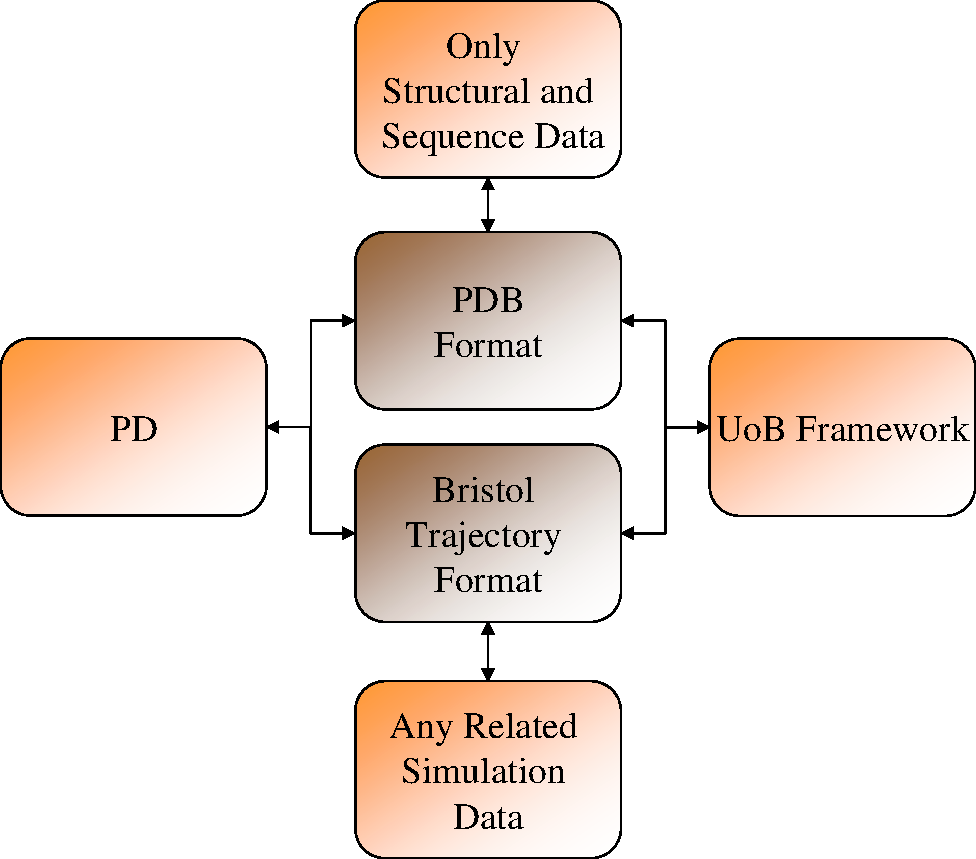
\includegraphics[width=0.5\textwidth]{03-Software/tra/tra.pdf}
\caption{Exchange and storage of data.}
\label{fig:software:tra}
\end{center}
\end{figure}


\subsection{Framework Structure}

The \uobf\  is highly modular in nature, comprising multiple  code assemblies which interact.\ These focus on the primary principles of flexibility and extensibility. The components can be rapidly intergraded into host applications for any given purpose, thus, the current implementation is used throughout this work. 

Figure \ref{fig:software:uobassemblies} illustrates that the \uobf\ is comprised of four primary \textsc{.Net} assemblies, each of which has a well defined role and is described in the following sections.

\begin{figure}[hptb]
\begin{center}
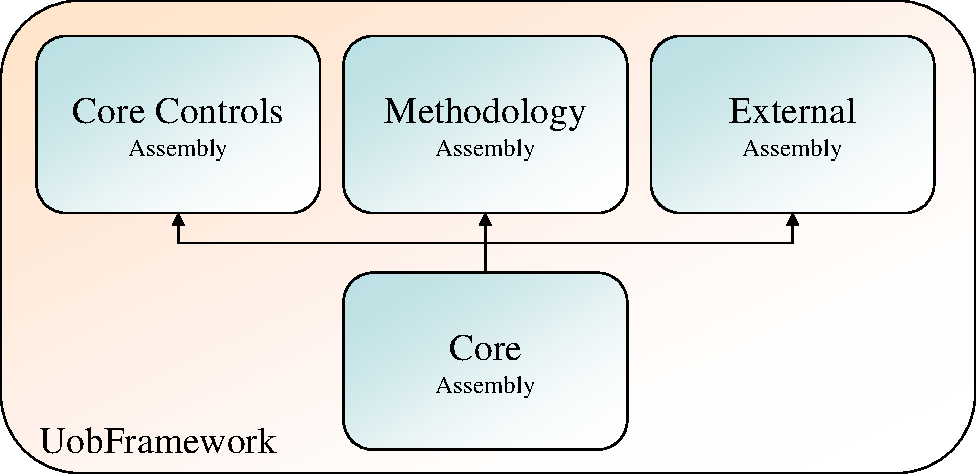
\includegraphics[width=0.5\textwidth]{03-Software/uobframework/assemblies.pdf}
\caption{The assemblies which compose the \uobf.}
\label{fig:software:uobassemblies}
\end{center}
\end{figure}

\subsubsection{The Core Assembly}
\label{section:software:uob:core_assembly}

Figure \ref{fig:software:uob:Core} shows a conceptual map of the functionality present within the core assembly of the framework. Structure and sequence data can be imported using functionality in the FileIO namespace. Development has focused on protein structures, however it could be easily extended to define other molecule types such as nucleic acids. Implemented structural manipulations include the rebuilding of missing atoms from library definitions and structural truncation and concatenation. Both structural and sequence alignments are available along with common functionalities like calculating sequence identities and \crms\ values. The data namespace is dedicated to the processing, statistical analysis and export of data. Finally, a number of additional tools are provided to simplify common labour intensive tasks. 

\begin{figure}[hptb]
\begin{center}
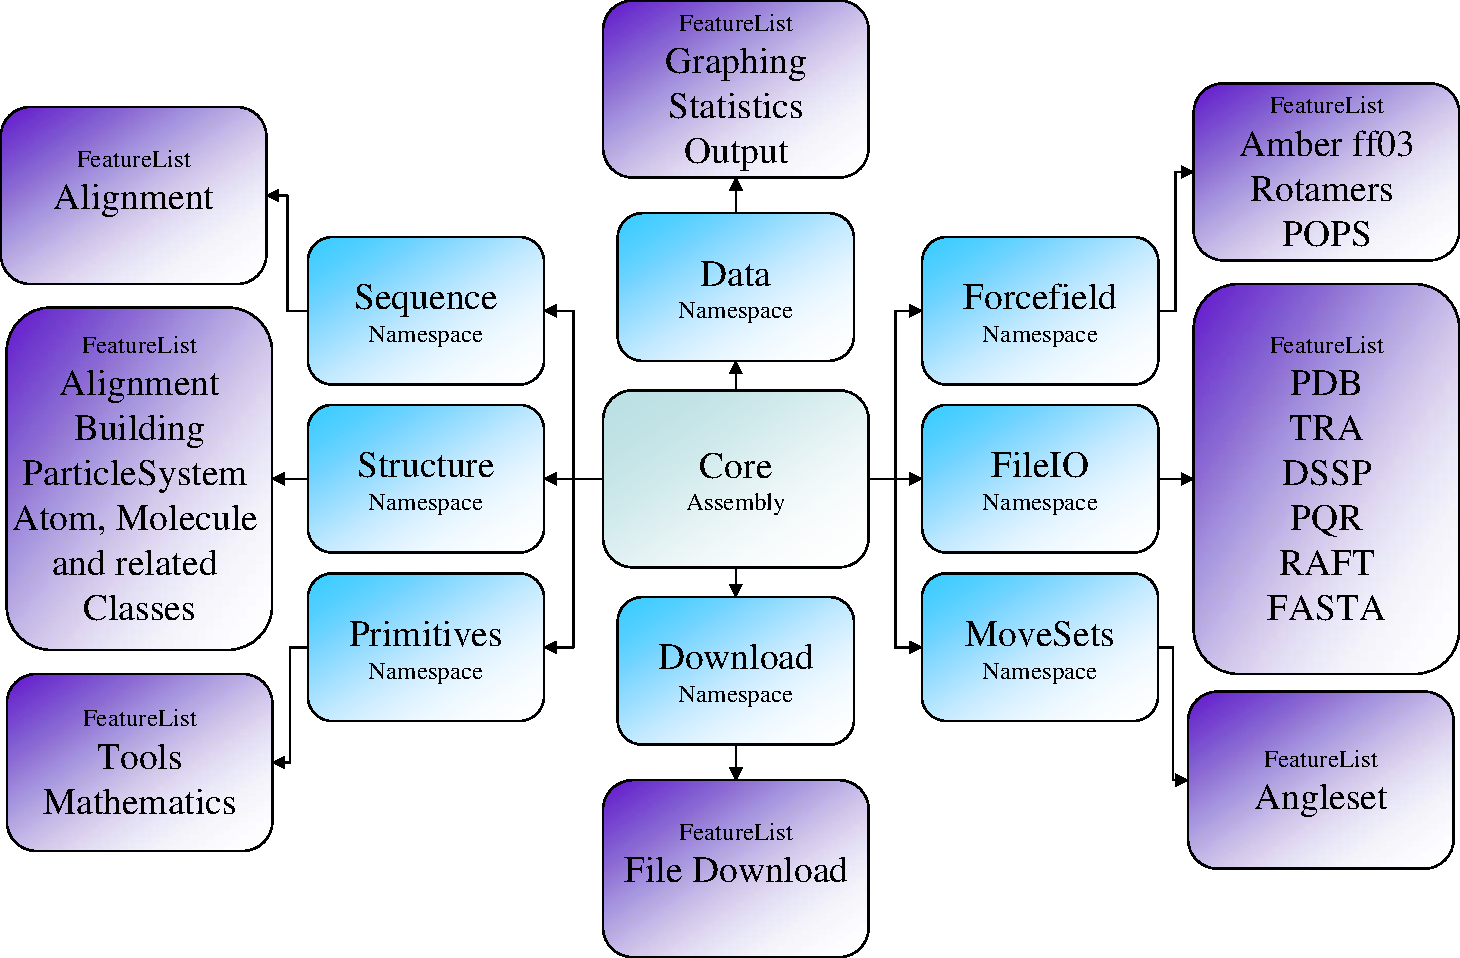
\includegraphics[width=0.75\textwidth]{03-Software/uobframework/core.pdf}
\caption{The component namespaces of the Core assembly and associated functionality.}
\label{fig:software:uob:Core}
\end{center}
\end{figure}

\subsubsection{The Core Controls Assembly}
Figure \ref{fig:software:uob:CoreControls} shows a conceptual map of the functionality present within the Core Controls assembly, which contains the visual components for user interaction with the Core assembly. This can be utilised by any application to allow user interaction with the underlying molecular data. Data visualisation is highly useful when analysing the large data sets that are typically produced during simulation.
The main included components are the molecular render controller and tool windows to control it; an associated OpenGL 3D graphics engine; and tool windows to control and display the underlying trajectory and  its data.
Each of these link together in a logical network, triggering each other to update as data is changed. For example, when the current trajectory position is changed using a trajectory control, it will  result in any linked OpenGL\ window refreshing to display the corresponding coordinates. 

\begin{figure}[hptb]
\begin{center}
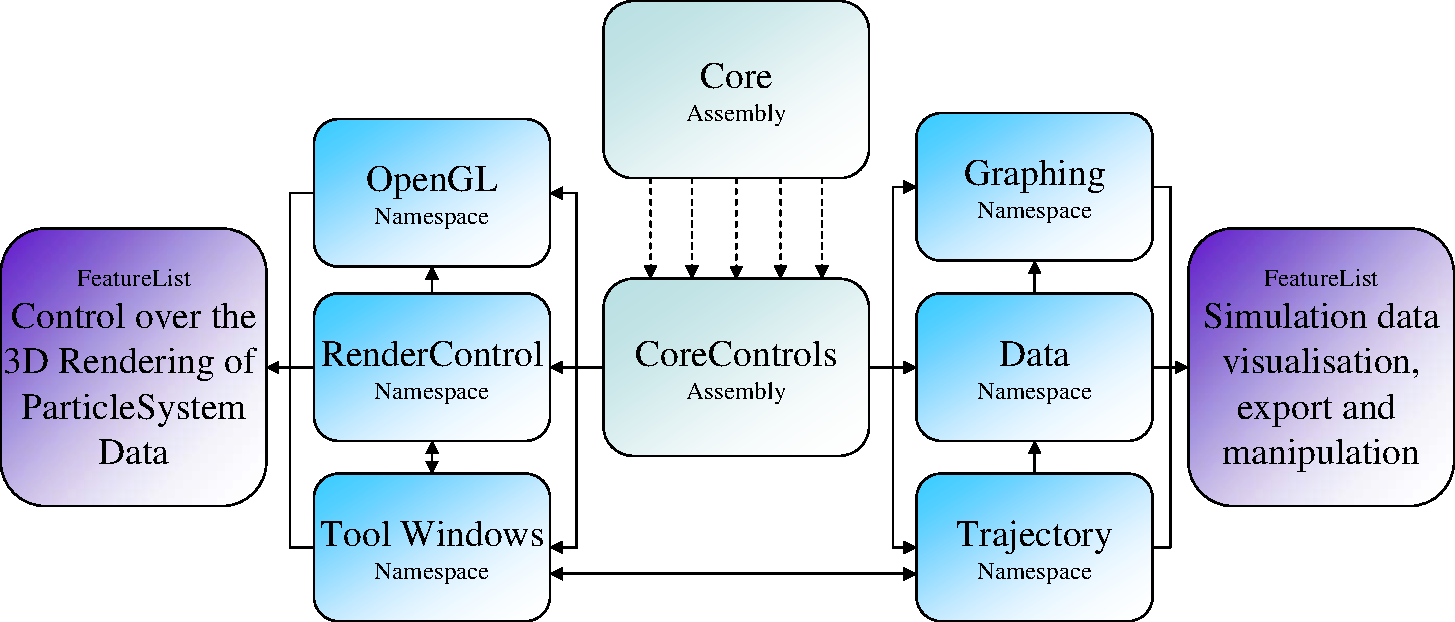
\includegraphics[width=0.75\textwidth]{03-Software/uobframework/corecontrols.pdf}
\caption{The component namespaces of the Core Controls assembly and associated functionality.}
\label{fig:software:uob:CoreControls}
\end{center}
\end{figure}

\subsubsection{The External Assembly}
The external assembly allows the \uobf\ to interactively distribute tasks to external applications. These applications are invoked asynchronously and their progress and data output is monitored. An example is the ability to launch an energy minimisation in \pd. By combining this with the core controls assembly, the   progress of the minimisation can be displayed and  minimised structure automatically imported for analysis. The external assembly also contains wrapper-code for a free file compression utility, therefore providing  an in-code user-friendly interface to any data stored within compressed files.

\subsubsection{The Methodology Assembly}
\label{section:uobf:methodology}

The Methodology assembly, shown in figure \ref{fig:software:uob:Methodology}, concerns the encapsulation a given task
into a class which derives from \textsl{TaskDirectoryInteration} and a set of complementary child classes. Each of these individual tasks is based around a single file-system folder  -- termed the Task Directory -- which may contain one or more libraries, a script generation folder, a result folder and a report folder. This system has been used throughout many of the developments in this work, including those in chapters \ref{chapter:database}, \ref{chapter:reduced_rep}, \ref{chapter:casp} and especially in \ref{chapter:methods}. Each application or application sub-mode uses a single Task Directory and performs its current operation upon it -- whether that be generating scripts to submit a simulation to a computer cluster, verifying produced data, fitting functions to data or producing reports based upon simulation output.

As discussed later in section \ref{section:loopcriterion}, \dssp\ has been used as the secondary structure annotation application throughout this work. As such, a common base class named \textsl{DSSPTaskDirectory} was derived from \textsl{TaskDirectoryInteration}, which is concerned with tasks that use a \dssp\ file library. Each of these tasks analyses some property that is contained within \dssp\ files, usually the \dssp\ secondary structure annotation, but sometimes useful auxiliary information such as \phipsi\ angles, SASA and per-residue temperature factor.


The final namespace is used to interact with a third party application called Origin, used to produce publication-quality statistical graphs. The classes within this namespace interact with the Origin's COM interface
in order to automatically produce reports containing graphs.
An example of such use is figure \ref{fig:intro:ramachandran}, which was actually originally part of an automated per-residue-type Ramachandran distribution analysis. The software engine for this analysis is contained within a class which derives from \textsl{DSSPTaskDirectory}. This then uses the Origin namespace to automatically produce both contour and scatter Ramachandran plots from the current database.

\begin{figure}[hptb]
\begin{center}
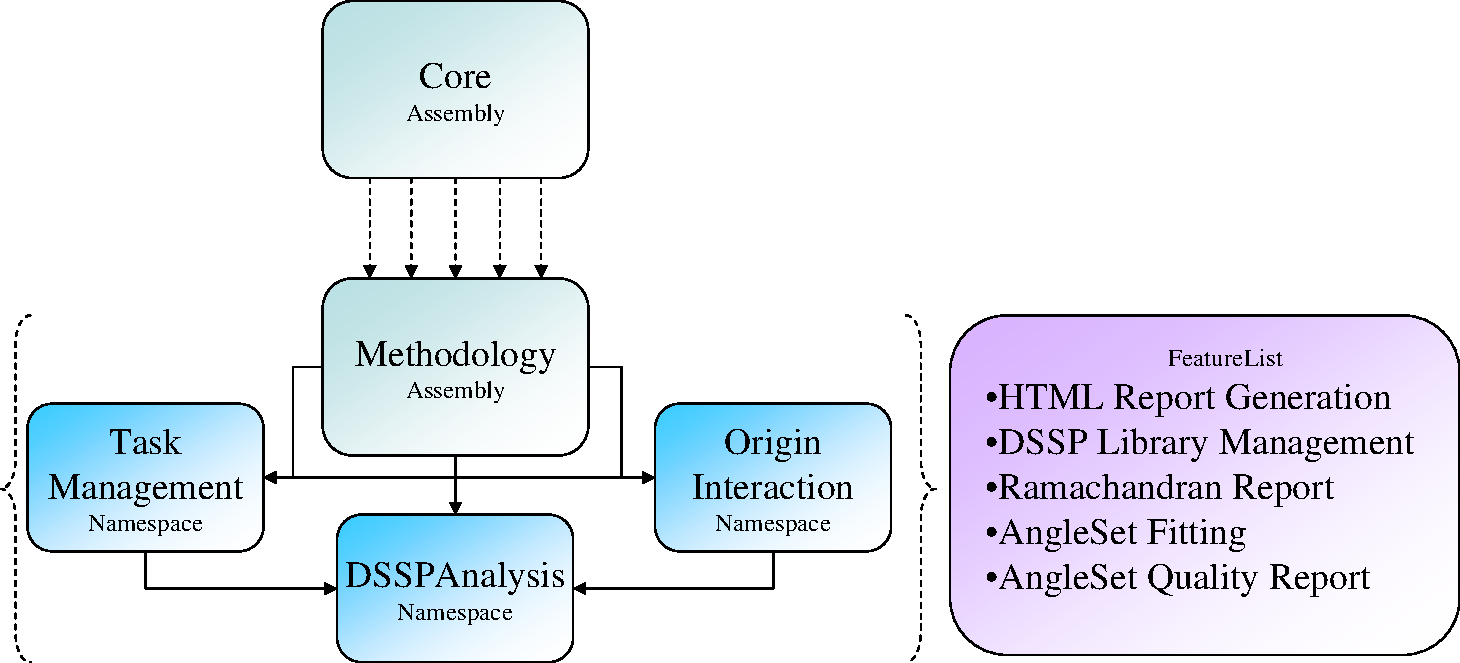
\includegraphics[width=0.85\textwidth]{03-Software/uobframework/methodology.pdf}
\caption{The component namespaces of the Methodology assembly and associated functionality.}
\label{fig:software:uob:Methodology}
\end{center}
\end{figure}

\subsection{Developed Applications}

Many applications have been developed which use the functionality contained within the \uobf\ and are listed in figure \ref{fig:software:uobapps}. These are discussed in detail in the relevant chapters of this dissertation. \dave\ is discussed briefly in the following section. A structural database creation engine named \pdbdb , is discussed in chapter \ref{chapter:database}.
The applications for \angleset\ viewing and fitting are discussed in chapter \ref{chapter:reduced_rep}. Finally, the ``Method Calibration'' software plays a critical role in chapter \ref{chapter:methods} -- without such software, the analysis would have been reduced to a convoluted set of hard-to-document shell scripts with poor error-checking.



\begin{figure}[hptb]
\begin{center}
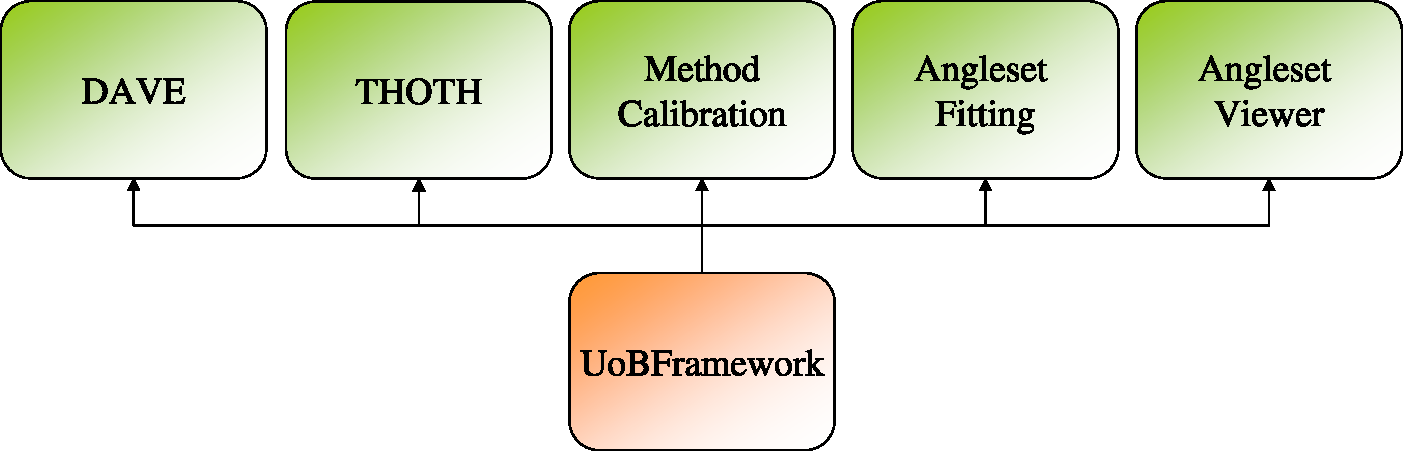
\includegraphics[width=0.8\textwidth]{03-Software/uobframework/apps.pdf}
\caption{The developed applications which rely on the \uobf.}
\label{fig:software:uobapps}
\end{center}
\end{figure}



\subsubsection{DAVE}

\dave, or Dynamic Atomic Visualisation Environment, is intended as a viewer of simulation data in its structural context. Importantly, \dave\ is not intended for use in the production of publication-quality molecular graphics, as there are many superior applications for this purpose. Instead \dave\ primarily deals with PDB and Bristol trajectory format files.

\dave\ possesses chemical knowledge of the molecules it is displaying, derived from a \pd\ format forcefield parameter file containing the \amberff\ definitions. As such, unlike in other viewers which must guess atomic connectivity and hence show incorrect bonding when close atomic contacts are present (common in unrefined models), \dave\ always displays the correct atomic connectivity. \dave\ can also display a tree-view for easy visualisation of any present polypeptides and provides drawing controls to change their appearance in the 3D display, both of which are side-bars in figure \ref{fig:software:davemain}. 

Any stored simulation data can be displayed directly in a simple data box, plotted graphically (figure \ref{fig:software:davegraph}) or exported in .csv format to applications like Microsoft Excel or Origin for further analysis. If the file was generated by \pd, there is also the option of displaying additional coloured vectors on the screen to represent arbitrary  aspects of the simulation. These lines are defined by the simulation and stored within the Bristol Trajectory format file. An implemented use of these lines is in displaying the force vector on each atom. They could also be used to display artificial inter-atomic restraints used during the simulation which are not part of the standard forcefield.

In addition to displaying pre-calculated information, \dave\ is also capable of its own analysis. One such display, which is generated on-the-fly, is the dynamic Ramachandran plot shown in figure \ref{fig:software:davemain}. As the current displayed simulation frame changes, the \phipsi\ angles are updated in the plot. 

Finally, \dave\ provides some more advanced tools including the ProSup structural alignment protocol\cite{COMPCHEM:ProSup}, launching an energy minimisation in \pd, displaying aligned sequence information and finally, a facility to rebuild missing atoms.

\begin{figure}[p]
\begin{center}
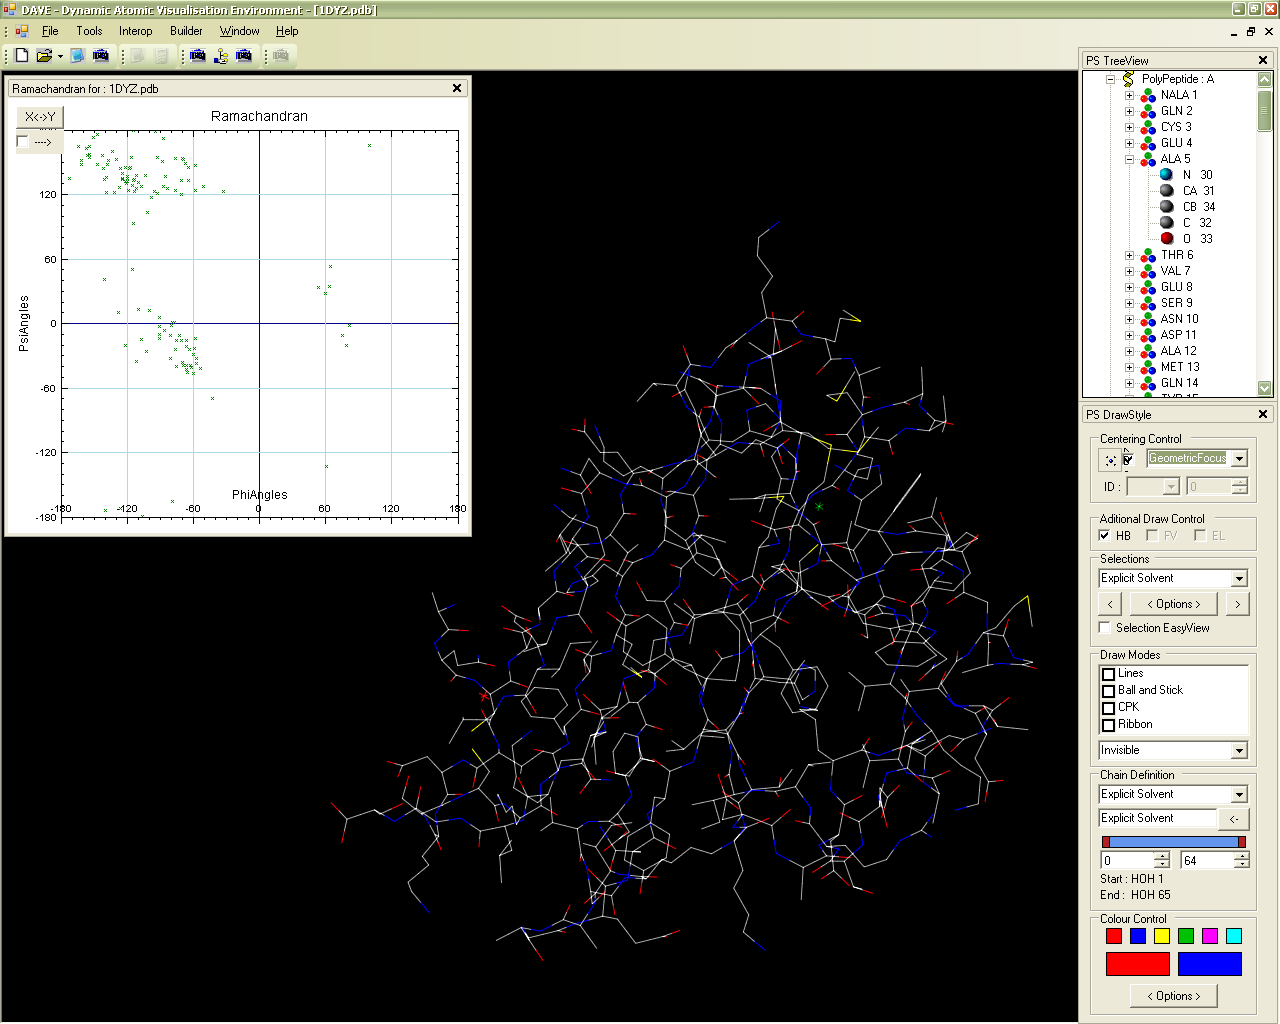
\includegraphics[width=0.75\textwidth]{03-Software/dave/main.png}
\caption{\dave: shown with a protein view, a tree-view representation of the atoms present, graphical options and dynamic Ramachandran plot.}
\label{fig:software:davemain}
\end{center}
\end{figure}

\begin{figure}[p]
\begin{center}
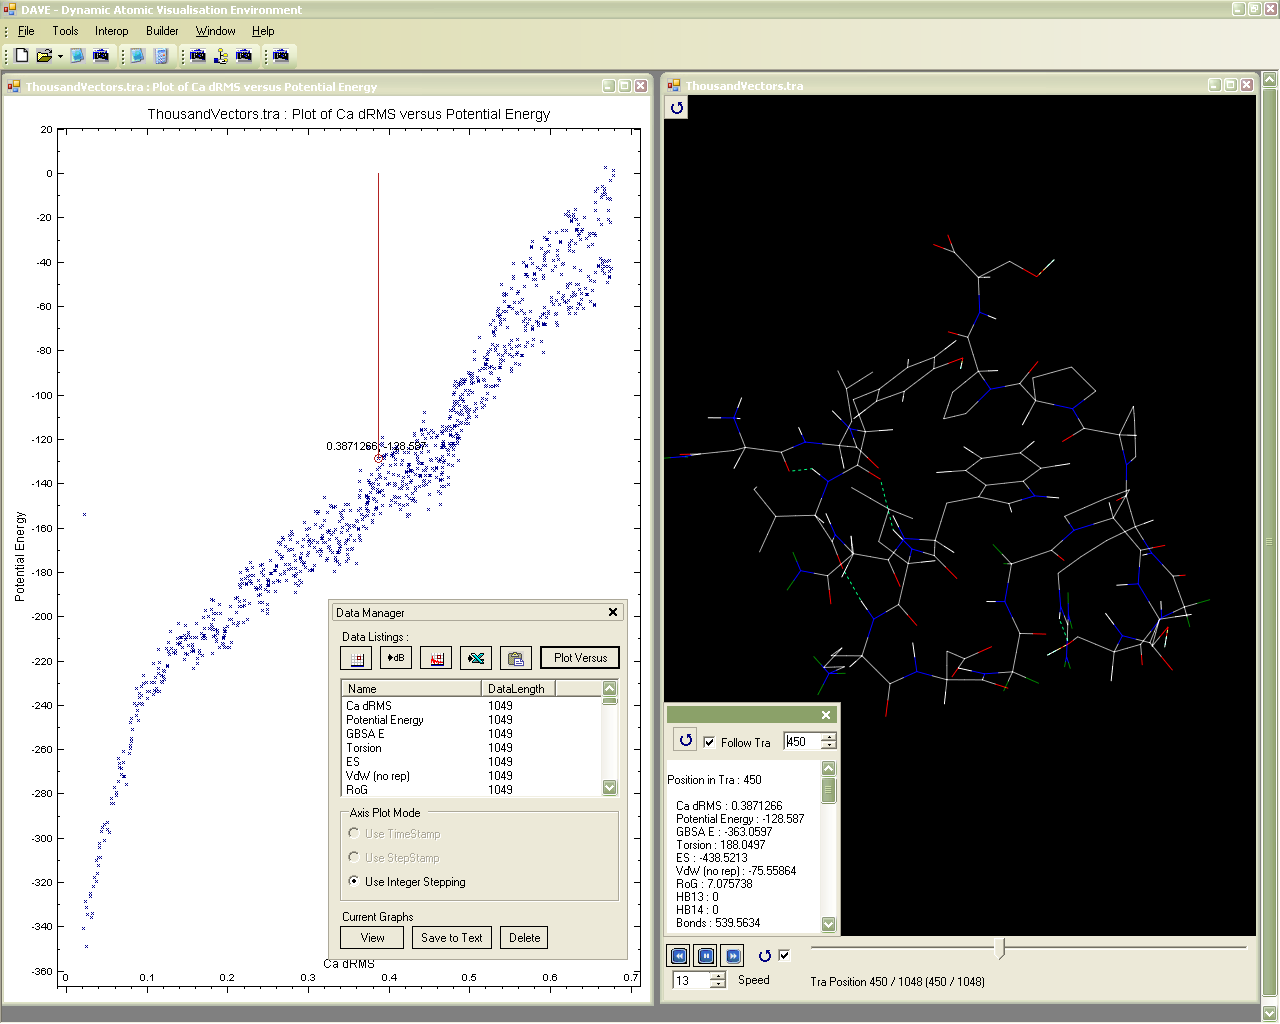
\includegraphics[width=0.75\textwidth]{03-Software/dave/graphing.png}
\caption{\dave: shown with a simulation of the TrpCage mini-protein and associated data. This includes a plot of energy vs. \ca-RMSD and a dynamic per-frame data box.}
\label{fig:software:davegraph}
\end{center}
\end{figure}

\subsection{Concluding Remarks}

The current implementation of the \uobf\ includes 55,497 lines of \CS\ source code, including 30,973 for the Core assembly, 18,169 lines dedicated to user interface components and just 5,961 lines dedicated to analysis tools. The relatively small amount of code dedicated to analysis stems form the concise interface that the framework core provides to its functionality. This is also represented by the fact that \dave\ and \pdbdb, although exhibiting significant functionality, are written in only 3,225 and 956 lines of code respectively.
It is clear that many other new scientific applications could potentially benefit from this shared base-code.
\clearpage
\section{Conclusions}

For this work two complementary frameworks have been developed to aid both molecular simulation algorithm development and data mining, totalling over 126,000 lines of code. This software, whilst still in rigourous development, is beginning to mature and as such is of real potential benefit to the research community. Both frameworks are soon to be made publicly available with a free academic licence. In terms of simulation, it is hoped that by combining a vast wealth of functionality into a single framework with a powerful front-end, the historical practise of having multiple small applications with separately maintained and overlapping functionality will be stemmed.  




         %  3. Software Framework Development
%&latex
\chapter{A Protein Structure Database}
\label{chapter:database}

\begin{quote}
``Chance favors the prepared mind.'' \\
--- \textit{Louis Pasteur}
\end{quote}

\section{Introduction}

The Protein Data Bank\cite{NATIVE:PDB:A,NATIVE:PDB:B,NATIVE:PDB:C,NATIVE:PDB:D} (PDB) is a large database of  experimentally derived protein structures, which at the time of writing contains 43,045 entries (table \ref{table:db:pdb}). There is significant redundancy within the PDB, such as structures of single-point mutants and multiple versions of a given protein in complex with different ligands.  In order to perform any meaningful statistical analysis on the sequence-structure relationships within the PDB, a non-redundant set is required.

Critical investigation of protein modelling methodologies requires such an idealised data set for the purpose of calibration and testing. To this end, two databases have been created in this work. The primary database is a subset of the entire PDB and is intended to be a representative set of all known protein structures to date. This \dataset\ facilitates statistical analyses of protein structure and acts as a \testset\ for protein modelling. Derived
from this database is a representative set of medium to long length loop structures for use in
the calibration and benchmarking of loop modelling methods.

\begin{table}[htbp]

\begin{center}
\begin{small}        
\begin{tabular}{+c^c^c^c^c^c}

\toprule 
\rowstyle{\bfseries} Experimental & \multirow{2}{*}{Proteins} & Nucleic Acids & Protein/NA  & \multirow{2}{*}{Other} & \multirow{2}{*}{Total} \\ 
\rowstyle{\bfseries} Method       &          & (NA)          & Complexes &       & \\
\midrule
   X-ray    & 34,017 &   963 &  1,570 & 28 & 36,578 \\
   NMR      &  5,346 &   753 &    129 &  7 &  6,235 \\
   EM       &     97 &    10 &     38 &  0 &    145 \\
   Other    &     80 &     4 &      3 &  0 &     87 \\
\midrule
   Total    & 39,540 & 1,730 &  1,740 & 35 & 43,045 \\
\bottomrule

\end{tabular}
\end{small}
\end{center}

\caption{PDB holdings breakdown: 27\superscript{th} April 2007.}
\label{table:db:pdb}

\end{table}


\section{Caveats of Atomic 3D Structure}
\label{DB:NativeProbs}


In nature, protein structures are highly dynamic and heterogenous entities in aqueous solvent\cite{NATIVE:Frau1991}. They are known to show
anisotropic motion and exhibit discrete conformational sub-states, the dynamics of
which can be functionally important\cite{NATIVE:DePristo2004}.
Surface loops, which have the least contact with the rest of the fold can exhibit structural transitions.
These include both rare transitions between competing isoenergetic minima and large structural fluctuations around a single minimum, termed static and  dynamic disorder respectively.

Traditionally, it is usual to represent proteins as a single structure unless strong evidence exists to support specific
multiple conformational sub-states. The majority of reliable publicly available experimental data is therefore published
as single structural representations. It is unfortunately not usual to quantify perceived uncertainty by showing valid conformational sub-states. In more recent times there have been
calls to halt this trend, by rejecting the practise of using single models,
in favour of representative ensembles\cite{NATIVE:Terwilliger2006}. This would particularity benefit models with regions of low certainty and would provide greater clarity for applications such as drug docking
and surface loop prediction.

For the time being, however, PDB \subsets\ can only be derived from the data contained
within the PDB itself. This work will therefore utilise a single native state
for each polypeptide chain, with the caveat that only those where there is high
structural certainty should be included. This practise
also simplifies structural analysis as it would be difficult to score
a given model structure against an entire ensemble.  \subsection{ NMR Spectroscopy for Proteins}

NMR, or Nuclear  Magnetic Resonance, has been used successfully to determine around 13.5\% of the PDB entries to atomic detail. Briefly, in NMR, a concentrated protein solution is prepared and usually multiple complementary NMR spectra are obtained. From these spectra, resonances are assigned and a series of spatial constraints are generated.
These constraints include distance restraints from NOESY spectra, angle constraints from coupling constants and orientation restraints from residual dipolar coupling.
From the satisfaction of this constraint matrix, an ensemble of candidate structures can be generated
and validated. Figure \ref{fig:db:nmr} shows PDB entry 1A57 as a typical example of an NMR structure.


\begin{figure}[p]
  \begin{center}
  
  \subfigure[The Full Structural Ensemble]{\scalebox{0.65}{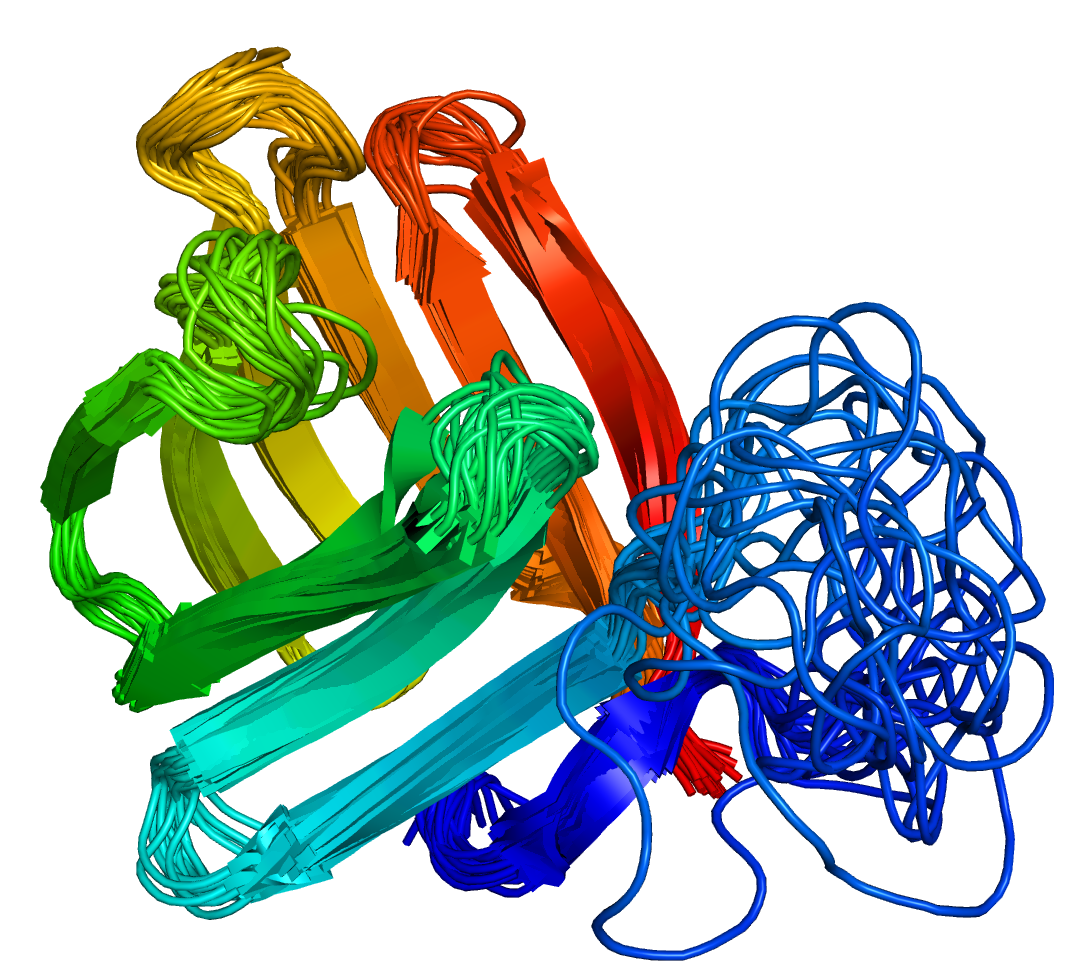
\includegraphics[width=1.0\textwidth]{04-Database/nmr/nmr_ensemble.png}}}
  \label{fig:db:nmr:a}
  \subfigure[Structural variation: Protein core \sidechains\ (Models 1-6 residues 33-36)]{\scalebox{0.75}{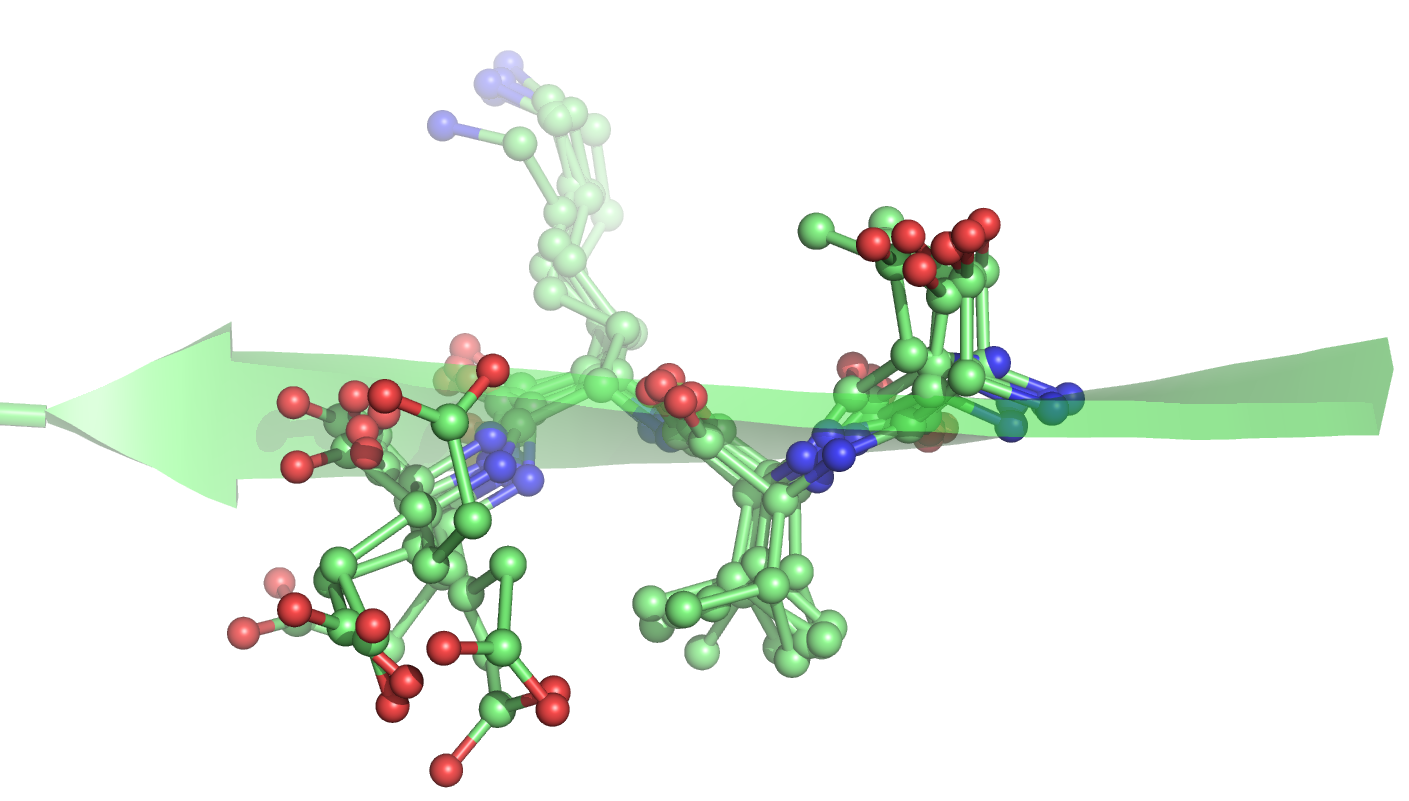
\includegraphics[width=1.0\textwidth]{04-Database/nmr/nmr_core.png}}}
   \subfigure[Structural variation: Surface \mainchain\ (Models 1-8, residues 98-111)]{\scalebox{0.75}{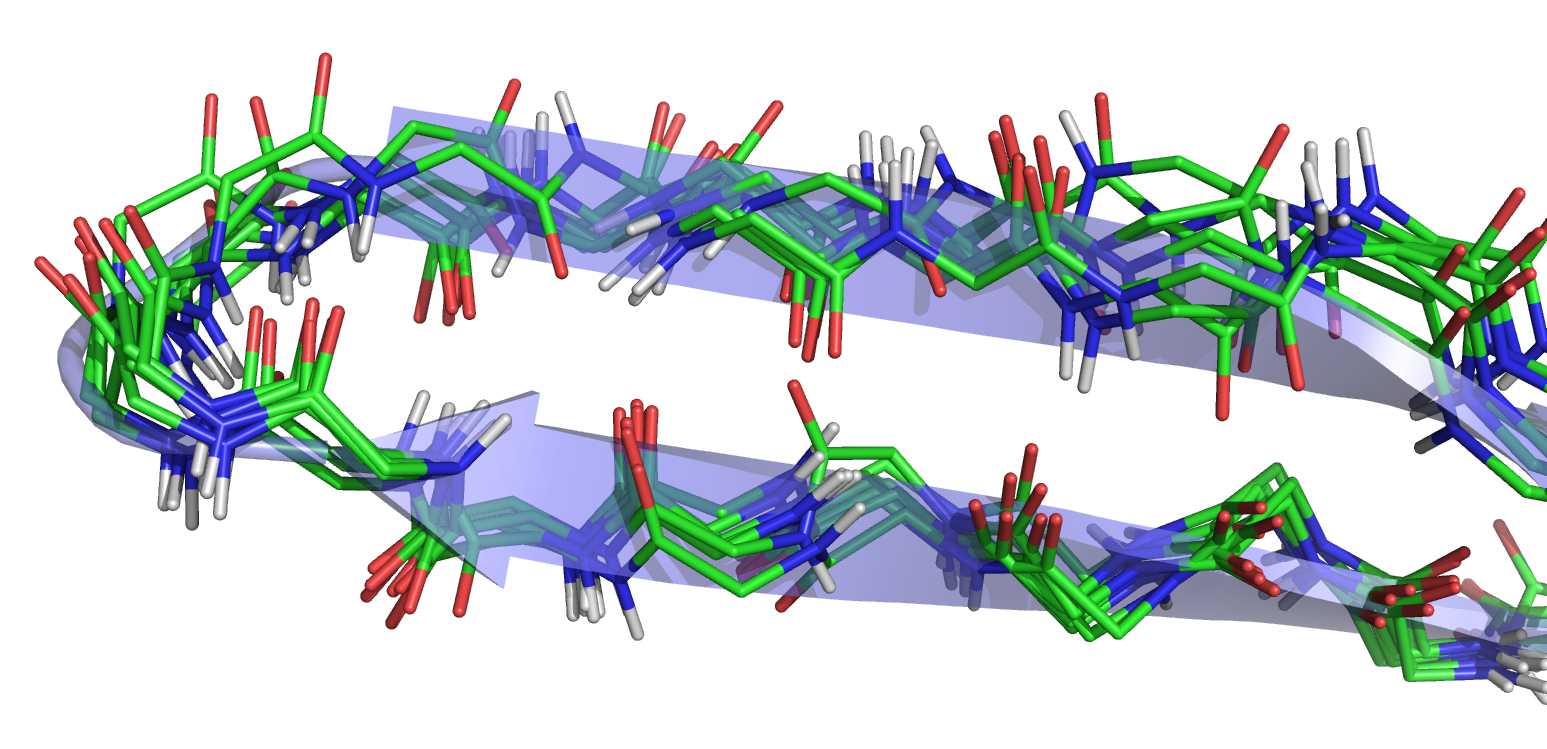
\includegraphics[width=1.0\textwidth]{04-Database/nmr/nmr_backbone.png}}}
      
    \caption[NMR Structure 1A57]{NMR structure 1A57, which contains 20 models.}
    \label{fig:db:nmr}
  \end{center}
\end{figure}



Originally most NMR structures were solved using metric matrix distance geometry (\mbox{\textsc{Diana}\cite{METHOD:DIANA:A,METHOD:DIANA:B}}), however current state of the art programs (\eg\ \mbox{\textsc{Xplor}\cite{NATIVE:XPLOR}}, \mbox{\textsc{Dyana}\cite{METHOD:DYANA:A,METHOD:DYANA:B}}) employ a combination of distance geometry and restrained molecular dynamics
(MD). MD has also been used in similar contexts such as protein model production from limited constraint sets\cite{METHOD:van94} and homology structure refinement\cite{METHOD:Fan2004}. Other NMR techniques have utilised conjugate gradient minimisation, molecular dynamics and simulated annealing in combination\cite{METHOD:Clo86}. There are however difficulties with the use of NMR structures within an idealised
PDB \mbox{sub-set}: 

\begin{enumerate} \isep
\item 
NMR data does not provide information about bonded
interactions, such as bond lengths and angles -- only non-bonded interactions are defined. The NMR restraint list therefore must included similar harmonic bond, angle and torsion terms to those in molecular mechanics \forcefields.
This in turn introduces structural bias if NMR derived information is used for benchmarking models produced using similar \forcefield\ terms. 

\item Most NMR structures are published as an \emph{ensemble} of valid structural states which satisfy the available restraints. There is however a large variation in the number of presented
structures in the ensemble from 1 up to 50, although most have around 20, complicating analysis of the ensemble. Some models are even presented as a single energy-minimised average
of all generated structural models, meaning that the information contained
within the ensemble is lost.

\item Following the satisfaction of the constraint matrix, there can still be large
deviations within the structural ensemble. This is exemplified by figures \ref{fig:db:nmr}-b
and \ref{fig:db:nmr}-c which show that both core \sidechains\ and surface \mainchain\
structures show significant deviations within the ensemble. 

\item Only protein segments for which restraints are present will have defined structure, often meaning that the N and C-termini and some more flexible surface loops will either have poor or no
structural definition in the final model \mbox{(figure \ref{fig:db:nmr}-a, blue C-terminal structure).} There is  no single standard for per-atom or per-residue quantification of structural certainty. Critically, therefore, such flexible regions are often present within the structure definition file, but sometimes have little quantification
of their certainty, making interpretation against
model structures difficult. Such scores could potentially be derived from
the structural ensemble and the original restraint list; The restraint list itself, however, is sometimes not published or of variable format. 

\end{enumerate}



Overall these facts make NMR data unsuitable for the work described in this
dissertation.





\subsection{X-Ray Crystallography}

Structures derived via \xray\ crystallography are currently the best standard available for benchmarking protein models. The majority are presented as single averaged structures and modelled with Gaussian, isotropic thermal motion. Each structure is an iteratively refined best fit of a structural model to available \xray\ diffraction data. There is, however, some debate about just how accurate and representative these structures are.
Automated refinement methods are in development\cite{NATIVE:DePristo2005,NATIVE:Adams2004}, but for the foreseeable future the majority of the PDB will have been produced using traditional crystallographic refinement, which is both labour intensive and directed by human judgement. 

Over 90\% of \xray\ structures diffract to $>$1.6\AA\ resolution, at the level where heterogeneity is hard to identify and model. It is thought that disregard for structural heterogeneity could cause difficulties in structural determination, as multiple isotropic models can explain the diffraction data equally well\cite{NATIVE:DePristo2004}.
More importantly, significant differences between these models shows that the accuracy of \xray\
crystallography for lower resolution structures is over-estimated as a whole.

Observed diffraction intensities are averaged over both space and time. Crystallographic B-factors, also known as temperature factors, are a measure of thermal motion of each atom and hence its structural
order.  If a group or single atom simultaneously occupies two isoenergetic positions within the unit cell, then they are said to have fractional occupancy; that is to say their position within the unit
cell is not constant. Selection of structures for a reduced PDB \jsubset\
should, therefore, take these two parameters into account.  

In a recent work comparing the 25 available non-isomorphous crystal forms of T4 lysozyme\cite{NATIVE:Zhang2004},
it was shown that varying crystal contacts perturb backbone atom positions by between 0.2\AA\ and 0.5\AA. Interestingly, the thermal factors of \sidechain\ atoms in individual structures correlate well with  the averaged values, whereas those for backbone atoms do not. This suggests that \xray\ structure thermal values are representative of \sidechain\ motion in solution, but not of backbone motion. This, in turn, shows that in some cases surface backbone conformation can be constrained by the crystal lattice. Such
findings are supported by other work on the effects of crystal packing\cite{METHOD:Plop:Jacobson2002A}.

Studies on the conformational quality of \xray\ structures often focus on
the Ramachandran map. As described in section \ref{section:intro:ramachandran}, the Ramachandran map can be conceptually divided into regions annotated ``allowed'' and ``disallowed'' based
on hard-sphere modelling of the protein \mainchain. This modelling is largely
successful as the bulk of the distribution lies within the allowed regions, however,
there are notable exceptions. These specifically include the disallowed population at $\Phi$ = 60\degree, $\Psi$ = -120\degree\ which is used in a \mbox{type II'} $\beta$-turn \cite{NATIVE:Gunasekaran1996}.
It is also noted that there are a number of \sidechain\ rotameric states which exist in small but structurally defined populations\cite{NATIVE:DePristo2004}. 

It is generally observed that scatter in torsional
distributions is reduced  as resolution improves, signifying an improvement
in overall stereochemical quality\cite{NATIVE:Morris1992}.
Multiple groups have however observed that lower resolution structures actually have a {\em lower} fraction of examples in the ``disallowed'' regions of conformational space. This rather counter intuitive observation suggests that the increased uncertainty in the placement of atoms in lower resolution structures causes the crystallographer to assume conformations lie within a high-propensity
region. In addition to this, other groups observe than many crystallographic structures contain
a small number of significant steric overlaps\cite{METHOD:Plop}; these discrepancies are both attributed
to incomplete model refinement.



\subsection{Summary}

In summary, \xray\ data is currently the best experimental source of  information available. The caveat of using these data is that one
has to assume that a given single high-resolution structure is truly representative of the underlying average  native
ensemble. In order to maximise the
confidence in a given test \dataset\ it is critical that stringent filter criteria for structural quality are applied. Such a filter should utilise per-structure
cutoffs for resolution and R-factor and per-atom cut-offs for temperature-factor and occupancy.
As the ambiguity is reduced by filtering such structures, this should minimise the level of bias introduced by human judgement within the selected \dataset. In terms of protein surface structure prediction, test cases should be chosen where the thermal motion of the surface atoms is minimal within  crystal structure and multiple degenerate \sidechain\ conformations do not exist. 



\section{Standardised PDB Subsets}

The overall aim of the work described in this chapter was to produce a refined subset of the PDB containing only representative polypeptide chains of high quality. Within this \dataset\ all structurally unique protein families should be represented. Several implementations exist in the literature with the ability to create culled PDB subsets by given criteria; all with respective advantages and disadvantages. 

The PDB itself can provide a set of sequences from a given query, culled at either 50\%, 70\%
or 90\% sequence identity; although for the purposes of this work the required single list of all \mbox{high-resolution} chains is not available.

\textsc{Cath}\cite{COMPCHEM:CATH,COMPCHEM:CATH:B} and \textsc{Scop}\cite{COMPCHEM:SCOP,COMPCHEM:SCOP02,COMPCHEM:SCOP04}
are the archetypal domain annotation implementations, providing lists of protein domains, as opposed to entire polypeptide chains. Flat file databases are available with structure quality annotations such as \xray\ resolution. The \textsc{Astral}\cite{NATIVE:ASTRAL} server provides lists of the \textsc{Scop} domain sequences culled at fixed sequence identity cutoffs or E-values derived from \textsc{Blast}\cite{SEQUENCE:BLAST} pairwise alignments. \textsc{Astral} also serves  PDB format files which correspond to the \textsc{Scop} protein domains.

The popular \pdbselect\ server\cite{NATIVE:Hob92,NATIVE:Hob94} had a widespread impact on statistical analysis of the PDB in the literature by providing pre-defined lists of chains with fixed maximum percentage sequence identities. \pdbselect\ follows strict selection criteria to produce its non-redundant protein database. The database is, however, not updated at any regular interval --
at the time of writing the most recent update of the 90\% identity list was March 2006.

\pdbselect\ functions by firstly removing all chains which do not fulfil
the ``Hard-Exclude'' criterion  (table \ref{table:db:pdbselect}).
An efficient sequence alignment algorithm\cite{SEQUENCE:Huang1991} is then utilised in order to group chains by respective pairwise sequence similarity. Chains which cannot be aligned over more than 10 residues are considered to be unrelated, irrespective of their sequence identity. Finally, the ``Soft-Exclude'' criterion is applied to the clustered groups and the best member picked by chain quality, scored using equation \ref{eq:pdbselquality}. 

\begin{table}[tbhp]
\begin{small}\begin{center}
\begin{tabular}{+c^r^p{0.6\textwidth}}
\toprule
\textbf{Exclude} &\multicolumn{2}{l}{\textbf{Description}} \\
\midrule
\textbf{Hard} 
&\textbullet& Length of $<$30 residues \\
&\textbullet& Number of non-standard amino acid residues (including chain breaks) more than 5\% chain length \\
&\textbullet& A resolution $>$3.5\AA \\
&\textbullet& An R-factor $>$30\% \\
&\textbullet& Some chains of known inferior quality \\
\midrule
\textbf{Soft} 
&\textbullet& Number of residues without \sidechain\ coordinates $<$90\% chain length \\
&\textbullet& Number of residues without backbone coordinates is $<$90\% chain length \\
&\textbullet& The content of alanine and glycine $>$40\% chain length \\
&\textbullet& No data on resolution or \mbox{R-factor} are available  \\
&           & (i.e. NMR-structures) \\
\bottomrule
\end{tabular}
\caption{The \pdbselect\ selection criteria.}
\label{table:db:pdbselect}
\end{center}\end{small}
\end{table}


\begin{equation}
\label{eq:pdbselquality}
\mathrm{Quality} = \mathrm{Resolution} + \left( \frac{\mbox{R-factor}}{20} \right)
\end{equation}

The \pdbselect\ implementation has many appealing quality control features, but is inherently not customisable
as it only provides two flat file lists at 25\% and 90\% sequence identity. This is problematic because 25\% would yield too few structures, whereas 90\% will yield highly redundant structural data, even for some surface loops. It also has the disadvantage of not facilitating the complete removal of NMR structures.
 
The \textsc{PDB-ReprDB} server\cite{NATIVE:Noguchi2000} provides a number of the features
which \pdbselect\ lacks, including the ability for the user to set parameters to generate customized lists \mbox{on-the-fly at any sequence identity cut-off}. The server also allows filtering
based on a wide range
of  criteria such as RMSD similarity and the exclusion of mutants, complexes and membrane proteins. \textsc{PDB-ReprDB} uses a Needleman �Wunsch global alignment algorithm\cite{SEQUENCE:Needleman1970} to provide its pairwise sequence identities.
It is updated approximately monthly.

\textsc{Pisces}\cite{NATIVE:Pisces:A,NATIVE:Pisces:B} is provided by the Dunbrack group. It supersedes their previous \mbox{\textsc{CulledPDB}} server and can provide lists culled from the entire PDB or from lists of PDB entries or chains provided by the user. It is updated more frequently than the other lists
at approximately weekly. Importantly for this work, \textsc{Pisces} provides a fine-grained array of pre-compiled chain lists using varying sequence criteria, R-value cut-off and resolution cut-off.

Critically, \textsc{Pisces} utilises PSI-BLAST\cite{SEQUENCE:PSIBLAST} 
with position-specific substitution matrices (PSSM), derived from NCBI's non-redundant protein sequence database\cite{SEQUENCE:Wheeler2005}, to obtain its pairwise sequence identities. The list is, therefore, intrinsically superior to other lists that utilise BLAST-like alignment as PSI-BLAST can identify longer evolutionary distance relationships, including  many below 40\% sequence identity, by aligning only well-conserved fragments. This, in turn, creates the longest lists currently possible of the highest resolution structures that fulfill the sequence identity and structural quality cutoffs.

In summary, \textsc{Pisces} has the overriding advantage of a superior sequence alignment at its core; The only disadvantage  is that, in order to filter against criteria such as chain length or number of chain breaks, the user must supply a custom source list to \textsc{Pisces} for culling or post-screen the pre-compiled lists. To this end, \textsc{Pisces} has been selected as the best option to provide the \basechainlist\
for this work. 

\section{The Protein Database}
\label{chapter:database:protein}

This section describes the development of the protein database used throughout this dissertation.

\subsection{Software Capabilities}

As described in section \ref{section:software:uob}, the \uobf\ suite was developed for the purpose of computational-biology file manipulation and data extraction. This allows the automatic, rapid and error-tolerant parsing and extraction of information from the notoriously inconsistent PDB format.
As such, it was the ideal candidate
for the basis for a small application to obtain and post-filter the \basechainlist. The application \pdbdb\ was developed, so named from the Egyptian god of record keeping, knowledge, and written language. \pdbdb\ itself contains very few code lines, depicting the significant functionality and flexibility of the \uobf\ as a code library for this type of application.

 
\pdbdb\ has the capability to not only post-screen PISCES chain-lists, but also those from \pdbselect, CATH and SCOP. As CATH
and SCOP provide structural classifications, these can be used to create
\subsets\ of a particular type of protein domain, simply by supplying the latest definition files and the appropriate class identifier. This additional functionality is available for future work, but is not used or described
further here. \subsection{Further Selection Criteria and Refinement}
% cullpdb_pc70_res1.8_R0.25_d060604_chains3359

The \basechainlist\ was obtained from \textsc{Pisces} on the 15\superscript{th} October 2006. This list is already assured to contain only  structures derived from \xray\ crystallography. From the selection of possible pre-compiled lists, a resolution cut-off of 1.8\AA,  an R-factor cutoff of 0.25 and a sequence identity cutoff of 70\% were chosen. A cut-off of 1.8\AA\ is far higher than 2.0$\to$2.2\AA\ which is often used in previous works\cite{METHOD:Modloop}. This ensures a very high quality of data
whilst maintaining a significant number of structures. It is worth considering that although structures with 70\% pairwise identity are expected to be  similar, most structural variability will be in surface regions, which are of particular interest in this work.
  For all these chains, the corresponding complete PDB file was automatically downloaded from the PDB  using the \pdbdb. The reduced \dataset\ used in this study needed to meet a number of greater quality standards than those in the \textsc{Pisces} chain-list itself. Multiple successive filters were utilised to remove inappropriate data for the purposes of creating a normalised set for protein simulation.

Non-standard residue types and indeed small chemical modifications to standard residues, require new \forcefield\ definitions and hence non-trivial \forcefield\ \mbox{re-parametisation}. This would be a significant amount of work to accommodate a small percentage of PDB entries and also impossible when using most applications
supplied by third\ parties. To accommodate these files, the first database refinement stage modified the residue definitions in the affected PDB structures. Firstly, any files containing multi-residue aggregates (table \ref{TABLE:DB:AGREDATES}), usually chromophores, were removed completely from the base chain-list.
Secondly, files containing either N-terminal acetylation or residues with 
minor \sidechain\ modifications were substituted with the standard base-residue. This was performed by utilising
the MODRES statements in the PDB file. The rationale behind this, is that these modifications are post-translational; hence, as a protein exits the ribosome, it will still fold stably when containing
only un-modified residues. In this work it is assumed that the overall protein structure will not be affected in any significant way by substituting standard residues. This defines the top-level refined structural database - the
\standardchainlist. 

\begin{table}[htbp]
\begin{center}
\begin{tabular}{+c^c^l^l}
\toprule
\rowstyle{\bfseries} PDBID & Residue & Chemical Nature & Involving \\
\midrule
 1OEW & SUI & Succinimide & Asp-54, Gly-55 \\
 2A46 & CR7 & Chromophore & Lys-68, Tyr-69 Gly-70\\
 2G6Y & CQR & Chromophore & Gly-58, Tyr-58, Gly-58 \\
 1ZGO & CRQ & Chromophore & Gln-66, Tyr-67, Gly-68 \\
 1W27 & MDO & Chromophore & Ala-202, Ser-203, Gly-204 \\
 2AWK & CRO & Engineered Chromophore & Ser-65, Tyr-66, Gly-67 \\
 2DDD & CR8 & Auto-Catalytic Chromophore & His-62, Tyr-63, Gly-64 \\
\bottomrule
\end{tabular}
\caption{Multi-residue aggregates present in PDB files.}
\label{TABLE:DB:AGREDATES}
\end{center}
\end{table}

The \standardchainlist\ was then put through two additional filters. Many simulations scale poorly with chain length, the first additional
filter therefore removes any chains $>$350 amino acids in length. This should avoid over-stretching computational resources, whilst still including multi-domain proteins.
Secondly, some computational simulation software deals poorly with missing atoms. By contrast  even \xray\ structures resolved to extremely high resolution often contain regions of missing electron density, especially amino acid \sidechains,\, but often complete surface loops.  The latter occurs because some surface loops exhibit significant dynamic behaviour. The second major filter therefore removes any structures that contain complete chain-breaks. This defines the \finalchainlist\ for use in this work. In
total 2,349 high quality chains were defined as shown in figure \ref{fig:db:cull_pie}.

\vspace{0.4cm}
\begin{figure}[hbtp]
\begin{center}
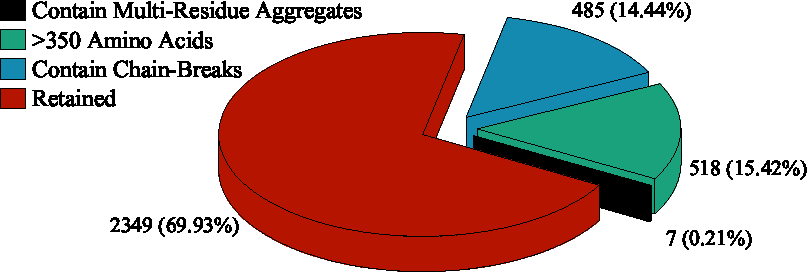
\includegraphics[width=0.8\textwidth]{./04-Database/CullPDBCounts/CullPDBCounts.pdf}
\caption{A summary of PDB structure culling for \thothdb.}
\label{fig:db:cull_pie}
\end{center}
\end{figure}

The final stage involved the structural refinement of the \finalchainlist\
using the functionality implemented in \pdbdb.
Missing \sidechain\ atoms were rebuilt using the highest propensity standard rotamer state which had minimal hard-sphere steric interaction with other defined atoms;  selected
from Richardson's penultimate rotamer library\cite{COMPCHEM:RICHARDSON}. Next, hydrogen atoms, which are missing from all \xray\ structures, were rebuilt using standard geometry as defined by \amber. 

As has been discussed in Section \ref{DB:NativeProbs} PDB structures sometimes contain atom positions in moderate steric overlap. In light of this, the structures were finally subjected to a short and gentle minimisation protocol
using the \pd\ simulation suite (section \ref{section:software:pd}). Thus,  any heavy steric clashes were removed, which could have caused simulations to fail or
behave unexpectedly. The gentle minimisation protocol used was extremely tolerant of any poor protein
geometry:\begin{enumerate} \isep
\item Minimise to a 0.1 \kcalmol\ energy gradient using \emph{only} the
standard \amberff\ bond, angle and torsion \forcefield\ terms. This will amend even extreme bond lengths without causing the minimisation to fail.
\item Minimise to a 0.1 \kcalmol\ energy gradient using the previous
\forcefield\ augmented with a soft-sphere steric \forcefield\ (figure \ref{fig:db:softvdw}).
This  results in atoms with heavy clashes moving gently away from each other until steric forces are satisfied. 
\item 
Finally, just 500 steps of minimisation were performed on the standard \ambergbsa\
\forcefield\ implemented in \pd. This ensured that electrostatic contacts were maintained whilst
the structure deviated little from its starting conformation.
\end{enumerate}
                   
                                 

\begin{figure}[hptb]
\begin{center}
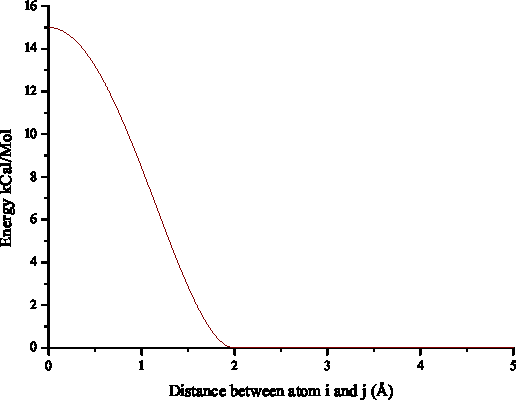
\includegraphics[width=0.5\textwidth]{04-Database/soft_sphere/potential.pdf}

\begin{equation}
E_\mathrm{softij}(h,x,d_\mathrm{ij},d'_\mathrm{ij}) = \left\{ \begin{array}{ll}
 h \left( 1.0 - \left(  d_\mathrm{ij}  / \left(  d'_\mathrm{ij} - x \right) \right) ^2 \right) ^2
  & \mbox{if $d_\mathrm{ij} < \left( d'_\mathrm{ij} - x \right)$ }\\
0 
  & \mbox{if $d_\mathrm{ij} \ge \left(d'_\mathrm{ij} - x \right)$ } \\
\end{array}
\right.
\end{equation}

\vspace{-0.5cm}

\begin{equation}
E_\mathrm{soft} = \sum^n_{i=1} \sum^n_{j=i+1} E_\mathrm{softij}
\end{equation}

\caption[The chosen soft-sphere potential]{The chosen soft-sphere potential,
where $h$ is the y-axis intercept which controls the hardness of the spheres
(default 15.0),
$d_\mathrm{ij}$ is the distance between atoms $i$ and $j$, $d'_\mathrm{ij}$ is the sum of their VDW radii (3.0 for the graph) and finally $x$ is an empirical  overlap tolerance
(default 1.0\AA). The calculation is summed for all atoms ($1\to n$) against
each atom with a higher numerical index.}
\label{fig:db:softvdw}
\end{center}
\end{figure}

As the minimisations were short, the minimised structures show a small all-atom \crms\ to the native structure, but some show a very significant difference in energy (figure \ref{datbase:minim}). The final mean, median and maximum
heavy-atom cRMS values for the 2,349 structures were 0.43\AA, 0.43\AA\ and 0.85\AA\ respectively.

\begin{figure}[htbp]
\begin{center}

\subfigure[Structural deviation following the gentle minimisation protocol
in an arbitrary typical section of the protein 
surface. The native and minimised structures are the blue and magenta respectively. ]{
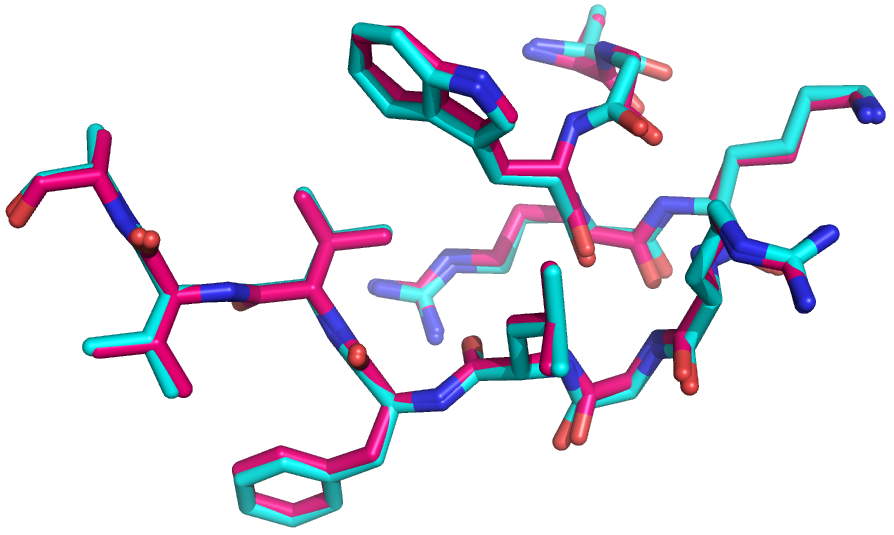
\includegraphics[width=0.75\textwidth]{./04-Database/img_protdb/MinStructureNoChange_zoom.png}}

\vspace{0.5cm}

\subfigure[The distribution of all heavy-atom \crms\ values between the native and \xray\ structures.]{
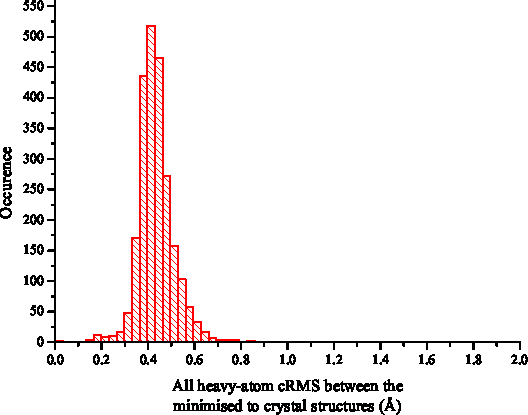
\includegraphics[width=0.75\textwidth]{04-Database/min_dev/MinimDeviation.pdf}}

\caption{Structural deviation following the gentle energy minimisation protocol.}
\label{datbase:minim}
\end{center}
\end{figure}


\subsection{Summary}

This section has described the process by which the PDB \jsubset\ for this
work was generated. For the task a specific application called \pdbdb\  was
developed which has the capabilities to both download the required PDB files
automatically and generate the required scripts to perform energy minimisation
using \pd. From this point, the resultant database of 2,349 high quality PDB structural files will be called \thothdb. 


\section{The Loop Database}
\label{section:intro:loop_db}

In true comparative modelling, a typical structurally variable region (SVR) or ``loop'' is usually defined as a region for which there is no discernible template sequence homology. In the majority of cases these regions  connect sections of regular secondary structure, but their exact bounds are dependent upon the method of sequence alignment,  the chosen template(s) and on the structural
alignment of those templates.
For calibration purposes in this study, the definition of a loop must be unambiguous.  Due to the close correlation between sections which span secondary
structures and those which are structurally variable between template structures, it was
decided that the loop definition of this work should be dictated by a solid secondary structure annotation algorithm.







\subsection{Secondary Structure Annotation}

In the past, secondary structure annotation was left to the structural biologist and was often inconsistent,
ambiguous and error prone. The advent of software applications for secondary structure annotation improved
this situation, however,
defining secondary structure from atomic coordinates alone is an inexact process due to differences in the exact definition used.
A study of three annotation methods exemplifies this by showing that on a non-redundant set of 154 proteins, all three methods agreed at only 63\% of residue positions\cite{NATIVE:Colloc1993}.
The choice of annotation method is, therefore, paramount as it is a cornerstone of the loop database definition
in this work.

\subsubsection{Annotation Methods}

\dssp \cite{NATIVE:DSSP}, or Dictionary for Secondary Structure Prediction, was released in 1983; implemented as a pattern recognition process of both geometric
and hydrogen bonded features and tested on a set of experimental coordinates. Overall, \dssp\ interprets \emph{cooperative} secondary structure from patterns of successive hydrogen bonded turns and bridges. Each residue is given one of a series of
characters  corresponding to its structural classification, shown
in table \ref{table:db:dssp}. \dssp\ is still seen today as one of the most consistent and accepted algorithms in secondary structure annotation and indeed bioinformatics as a whole; being cited in the scientific literature more than 1,000 times. However, alternatives do exist and were considered in this work. 

\begin{table}[hptb]
\begin{center}
\begin{tabular}{+c^l}
\toprule
\rowstyle{\bfseries}
     Code & Secondary Structure \\
\midrule
     H & \ahelix \\
     B & Isolated \be-bridge \\
     E & Extended strand, participates in \be-ladder \\
     G & 3\subscript{10}-helix \\
     I & $\pi$-helix\\
     T & Hydrogen bonded turn \\
     S & Bend \\
     -- & No structural annotation \\
\bottomrule
\end{tabular}
\caption{The secondary structure dictionary used by DSSP.}
\label{table:db:dssp}
\end{center}
\end{table}

In \dssp\ `E' is the annotation for a \bstrand. \dssp\ also allows \be-bulges to be assigned `E', allowing up to four residues on one side of sheet and one on the opposite side to be included in such a structure. The same is often not true of author annotations on the PDB \website\ or under other automated annotation methods. \be-bulges are, however, expected to be largely conserved between homologous structures.

\stride \cite{NATIVE:STRIDE} shows a number of similarities to \dssp\, but has a greater emphasis on backbone
torsions resulting in the inclusion of more residues at the termini of secondary structures.
\stride\ also adds an additional term in the expression of hydrogen bond energy,
which attempts to ensure planarity of the bond whilst allowing longer bonds to be included. Compared to \dssp, \stride\ tends to provide slightly
longer secondary structure annotations, although when compared pairwise, \dssp\ and \stride\ agree for approximately 95\% of residues\cite{NATIVE:Cuff1999}.

Part of the same method-family as \dssp\ and \stride\ is \secstr \cite{NATIVE::SECSTR}, which was developed
specifically to enhance the detection of $\pi$-helices. Unsurprisingly the
method therefore succeeds in categorising  additional structures to be $\pi$-helices when compared to \dssp. 

The method \define \cite{NATIVE:DEFINE} uses the distance separation between \ca\ atoms, variable between structure types, as its criterion for annotation. \define, however, has been shown to over-accommodate backbone distortion and therefore result in over-assignment of regular secondary structure. As a consequence \define\ assigns more than twice as many \bstrands\ of length four than most other methods\cite{NATIVE:Colloc1993}. \psea\ also relies solely on \ca\ coordinates and distance and angle criteria between
them\cite{NATIVE:PSEA}, but has been shown to largely agree with \stride \cite{NATIVE:KAKSI}.

\pcurve \cite{NATIVE:PCurve} is a third method type  which calculates
annotations using parameters like the tilt and roll between peptide planes. \pcurve\ also has a tendency to assign overly long elements of regular secondary structure. \xtlsstr\cite{NATIVE:XTLSSTR} analyses amide-amide interactions in an attempt to reproduce the same secondary structure annotations as would be derived by human visual inspection. \votap\cite{NATIVE:VOTAP} utilises Voronoi tessellation to produce contact matrices which are then used for annotation. 

Finally, \kaksi\cite{NATIVE:KAKSI}, one of the most recent additions to the field, uses both \ca\ distances and \phipsi\ angles during annotation, paying special attention to kink-detection in helices. Uniquely,
as annotation is sensitive to experimental determination method and resolution,
annotation parameters can be chosen dependent on the these properties. \kaksi\ was often shown to give several short secondary structures annotations with short breaks as opposed to a single large annotation. This generally results in fewer helix kinks and shorter more regular  secondary structures, which was an aim for the work.




\subsubsection{Structural Considerations for Annotation}


Residue geometry and hydrogen bonding patterns are less well defined towards the ends of regular secondary structures. That is to say, each amino acid still has similar backbone torsional angles, but those residues at either end of the structure often no longer exhibit hydrogen bonds.
This in turn means that, as sequence identity falls in comparative modelling, the ends of regular structures show significant variation  between multiple homologous templates.
In light of this, the \emph{under}-annotation of secondary structure length is preferable to over-annotation for the purposes of loop modelling calibration. On average,
this  yields longer loop definitions, but their use will result in a  fairer measure of the ability
of individual tools in real comparative modelling. 




\subsection{The Final Loop Definition}
\label{section:loopcriterion}

In summary, \dssp\ is still a solid bioinformatics standard and the most respected
annotation method currently available. Its annotations are typically shorter when compared to most other methods, however, this is desirable in this work
as the termini of secondary structures are the most structurally variable
in comparative modelling. \dssp\ also does not consider secondary structural
distortions like \be-bulges
to be separate structural types, which is again of benefit to this work as such structural distortions
are also expected to be  conserved. The use of DSSP should therefore ensure that the \dataset\ is especially representative of surface loops.
The exact loop definition used in this work is as follows:
\begin{enumerate}{} \isep
        \item  Using DSSP\cite{NATIVE:DSSP}, secondary structure annotation files were produced for non energy-minimised
PDB structures.        
        \item  ``Continuous'' regions of secondary structure are defined as a minimum of three residues of \bstrand\ (`E') or five residues of \ahelix\ (`H').
        \item  Loops are then defined as the connecting regions between these
continuous secondary structures, excluding the N and C-termini.       
        \item  Loops must be unbroken polypeptide in the available experimental data with all \sidechain\ heavy atoms
defined.
        \item  The standardised database itself does contain modified
residues which have been converted to standard residues. In contrast to this,
the loops themselves must \emph{not} have contained any modified residues
in the original PDB structure.

\end{enumerate}



\subsection{Loop Database Implementation}

As has been discussed, \thothdb\ represents a set of 2,349 high quality PDB and complementary \dssp\ files. The loop database itself is created on-the-fly by parsing the \dssp\ files as required. The inner details of the parsing process are encapsulated within a base-class called \textsl{DSSPTaskDirectory} which is present in the Methodology assembly of the \uobf\ as described in section
\ref{section:uobf:methodology}. Listing \ref{listing:db:dsspcode} shows that by deriving from this class, all the details of dealing
with this library of \dssp\ files and the subsequent extraction of information is abstracted away, leaving the user to deal solely with the problem at hand.


\lstset{language=CSharp}
\begin{lstlisting}[caption={Example code for \thothdb\ interaction.}, label=listing:db:dsspcode] 
// Derive a class from the base class `DSSPTaskDirectory' which
// embodies the abstract concept or parsing a folder of DSSP files
class Example_Thoth_DB_Client : DSSPTaskDirectory
{
    private static const int[] loopLengths = new int[] { 6, 7, 8, 9, 10, 11 };
    
    public void Execute()
    {
        // For each loop length we want to look at, run this loop...
        foreach (int loopLength in loopLengths)
        {
            ParsingFileIndex = 0; // reset IMPORTANT
            while (true)
            {    
                // *** The task we would like to perform ***
                SomeFunction( CurrentFile );

                // While we have further DSSP files, set CurrentFile to the next one...
                if (ParsingFileIndex < FileCount - 1) { ParsingFileIndex++; }
                else { break; } // Otherwise, break when we are done
            }
        }
    }
}

\end{lstlisting}

For each derived class, once the Execute() function has been added to the code, the object \textsl{CurrentFile} can be used. \textsl{CurrentFile} is an instance of the class \textsl{DSSPFile} and encodes all the
properties and information within a given \dssp\ output file. Listing \ref{listing:db:dsspoptions}
shows the three main function calls which can be made to \textsl{CurrentFile} dependent
upon the task at hand. For example, if the current task involves looking at loop structures, the function GetLoops() is called which returns all the loops
of the requested length(s) in the current \dssp\ file. These loops can then
be filtered and analysed as required by each individual task.

\lstset{language=CSharp}
\begin{lstlisting}[caption={Example code for DSSPFile class interaction.}, label=listing:db:dsspoptions] 
private void SomeFunction( DSSPFile currentFile )
{
    // Option 1) : GetResidues()
    // Perform analysis on individual resudues
    ResidueDef[] residues = CurrentFile.GetResidues();
    for (int j = 0; j < residues.Length; j++) 
              { DesiredFunction(residues[j]); } // act upon each residue


    // Option 2) : GetLoops()
    // Perform analysis on individual loops
    bool includeTerminii = false;
    bool validityFilter = true; // Remove unsatisfactory loops
    int loopLength = 8; // Include only 8-mers
    SegmentDef[] loops = CurrentFile.GetLoops(loopLength, includeTerminii, validityFilter);
    for (int j = 0; j < loops.Length; j++) 
              { DesiredFunction(loops[j]); } // act upon each loop


    // Option 3) : GetSecondaryStructures() 
    // Perform analysis on individual secondary structures 
    SegmentDef[] secStruc = CurrentFile.GetSecondaryStructures();
    for (int j = 0; j < loops.Length; j++) 
              { DesiredFunction(loops[j]); } // act upon each secondary structure
}
\end{lstlisting}

In this way, each given
task to be performed on the loop database can be easily encapsulated into a single
class. All of the analyses performed in chapter \ref{chapter:methods} are represented by
one or more of these classes which derive from \textsl{DSSPTaskDirectory} and utilise
the function call GetLoops().
 
\subsection{Loop Database Properties}
\label{section:loop_stats}

Following generation of the loop database in this work, structural features
were analysed and corresponding statistics generated. The difference in residue occurrence in all protein structure versus loop structure is shown in table \ref{table:database:propensity}, where in general the trends are as expected. The occurrence of hydrophobic residues is greatly reduced in surface
loops, whereas polar and charged residues are more prevalent. Proline, which
acts as a \mbox{helix-breaker} occurs 61\% more frequently in loop structure, whereas
helix-promoting alanine shows a 20\% reduction. Finally, due to its greater conformational freedom, glycine shows a 57\% increase in loop structure.
 
 

\begin{table}[htbp]
\begin{center}
\begin{tabular}[b]{+l^r^r^r^r^r^r}
\toprule
\rowstyle{\bfseries} 
 & \multicolumn{2}{c}{\textbf{All\ Structure}} & \multicolumn{2}{c}{\textbf{Loop\ Structure}} & Expected$^*$ & \% \\
\rowstyle{\bfseries} 
Residue / Class & Count & \multicolumn{1}{c}{\textbf{\%}} & Count & \multicolumn{1}{c}{\textbf{\%}} & \multicolumn{1}{c}{\textbf{Count}} & Difference  \\
\midrule
All Residues      & 733,048 & -      &  294,464   &  -      & -       & -                     \\
Charged           & 183,631 & 25.05  &  76,543    &  25.99  & 73,764  & 103.8   \\
Short Hydrophobic & 218,885 & 29.86  &  61,045    &  20.73  & 87,925  & \textcolor{red}{69.4} \\
Polar             & 183,629 & 25.05  &  80,642    &  27.39  & 73,763  & 109.3   \\
Bulky Aromatic    & 84,251  & 11.49  &  29,778    &  10.11  & 33,843  & \textcolor{red}{88.0} \\
Not Gly Or Pro    & 641,437 & 87.50  &  235,937   &  80.12  & 257,664 & \textcolor{red}{91.6} \\
Ala               & 61,446  & 8.38   &  19,849    &  6.74   & 24,682  & \textcolor{red}{80.4} \\
Arg               & 34,764  & 4.74   &  12,637    &  4.29   & 13,964  & \textcolor{red}{90.5} \\
Asn               & 32,510  & 4.43   &  17,887    &  6.07   & 13,059  & 137.0   \\
Asp               & 43,245  & 5.90   &  23,735    &  8.06   & 17,371  & 136.6   \\
Cys               & 10,653  & 1.45   &  3,861     &  1.31   & 4,279   & \textcolor{red}{90.2} \\
Gln               & 27,015  & 3.69   &  9,619     &  3.27   & 10,851  & \textcolor{red}{88.6} \\
Glu               & 46,337  & 6.32   &  16,312    &  5.54   & 18,613  & \textcolor{red}{87.6} \\
Gly               & 57,437  & 7.84   &  36,329    &  12.34  & 23,072  & 157.5   \\
His               & 16,921  & 2.31   &  7,377     &  2.51   & 6,797   & 108.5   \\
Ile               & 40,689  & 5.55   &  9,919     &  3.37   & 16,344  & \textcolor{red}{60.7} \\
Leu               & 63,696  & 8.69   &  17,987    &  6.11   & 25,586  & \textcolor{red}{70.3} \\
Lys               & 42,364  & 5.78   &  16,482    &  5.60   & 17,017  & \textcolor{red}{96.9} \\
Met               & 14,699  & 2.01   &  4,383     &  1.49   & 5,904   & \textcolor{red}{74.2} \\
Phe               & 29,478  & 4.02   &  9,643     &  3.27   & 11,841  & \textcolor{red}{81.4} \\
Pro               & 34,174  & 4.66   &  22,198    &  7.54   & 13,727  & 161.7   \\
Ser               & 44,551  & 6.08   &  22,238    &  7.55   & 17,896  & 124.3   \\
Thr               & 42,163  & 5.75   &  17,960    &  6.10   & 16,936  & 106.0   \\
Trp               & 11,115  & 1.52   &  3,681     &  1.25   & 4,464   & \textcolor{red}{82.5} \\
Tyr               & 26,737  & 3.65   &  9,077     &  3.08   & 10,740  & \textcolor{red}{84.5} \\
Val               & 53,054  & 7.24   &  13,290    &  4.51   & 21,311  & \textcolor{red}{62.4} \\
\bottomrule
\end{tabular}
\end{center}
\caption[\thothdb\ residue occurrence statistics]{\thothdb\ residue occurrence statistics: Observed and expected residue propensities are compared between all types of structure and loop structure only. 

$^*$The expected counts are theoretical extrapolations
created by multiplying the observed \%\ occurrence of each structural class by the total
number of loop total number of residues found in loop structures (294,464). Of course, as loop structure exhibits alternative residue propensities, the
observed occurrence is different. A reduction in residue propensity in loop regions is illustrated by
a red value in the
\% difference column.}
\label{table:database:propensity}
\end{table}




The distribution of loop lengths is shown in figure \ref{fig:Loop_DB_Hist},
where the majority of loops are under eight residues in length; although longer loops
of up to twelve residues are still very significant in number. Most of the ultra-long loops are highly convoluted regions containing only very small regions of secondary structure outside the definition used in this work. An example of this is shown
in figure \ref{fig:LDP_LongLoop} which depicts a \mer{56} surface region of 1AFWB where only two short regions of secondary structure exist and regular hydrogen bonding is minimal. The Ramachandran plot for this fragment shows some \mainchain\ torsional angles are on the outskirts of the normal Ramachandran regions.

\begin{figure}[htbp]
\begin{center}
    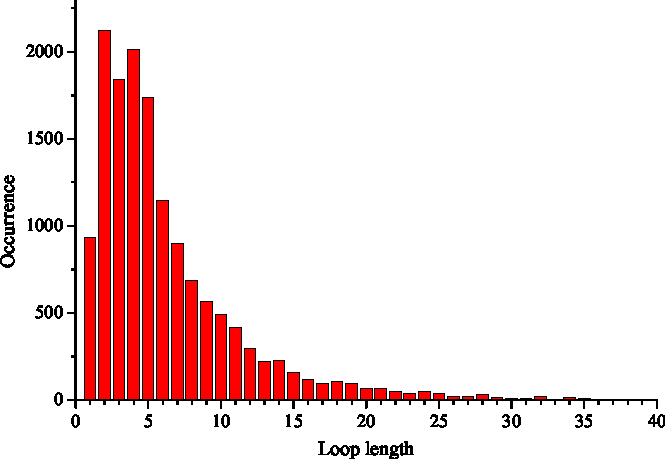
\includegraphics[width=0.8\textwidth]{./04-Database/img_loopdb/loop_length.pdf}
    \caption{Histogram showing the distribution of loop lengths resulting from the
chosen loop definition.}
    \label{fig:Loop_DB_Hist}
\end{center}
\end{figure}

\begin{figure}[htbp]
\begin{center}
  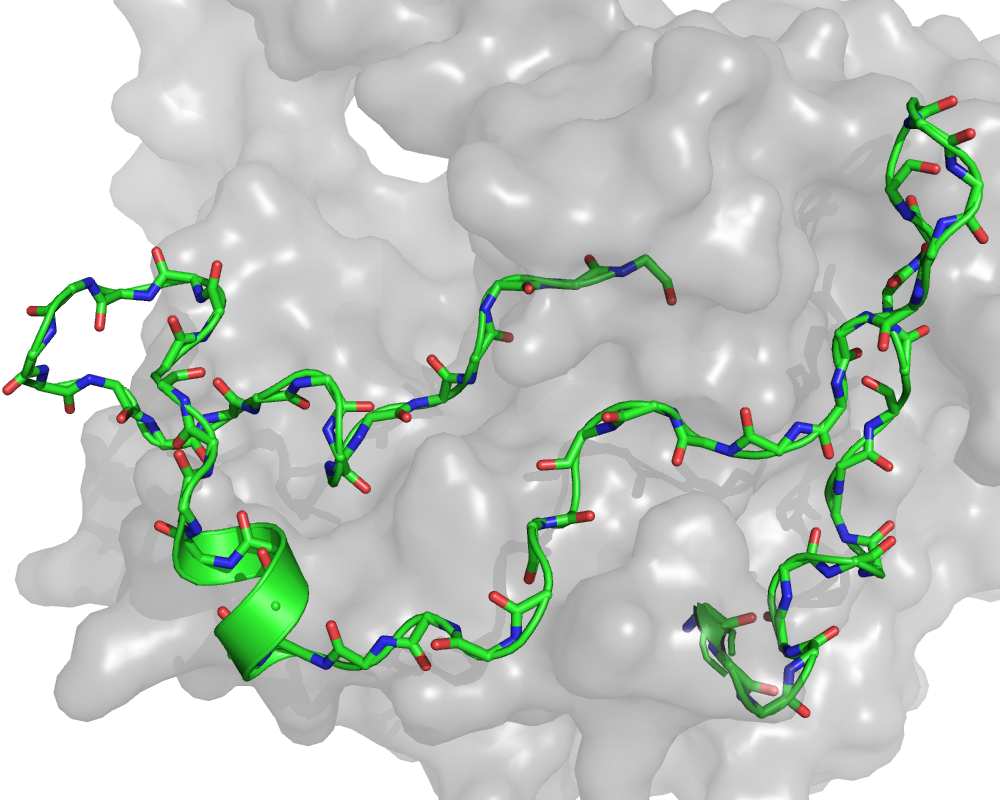
\includegraphics[width=0.8\textwidth]{./04-Database/img_loopdb/longloop.png}
  \newline                
  \mbox{ \small{DSSP Descriptor\cite{NATIVE:DSSP}}: \tiny{`TTTTTTTB--EE-TTS-EE-S-S---TT--HHHHTT---SSSTTT----TTSB---'}}
  \caption[A convoluted \mer{56} compound loop]{A convoluted \mer{56} compound loop taken from 1AFWB comprising of residues 221 to 276. Image created with \pymolV.}  
  \label{fig:LDP_LongLoop}
\end{center}
\end{figure}

This study focuses on medium to long  loops, which for the purposes
of this work will be defined
as those containing between 6 and 12 residues. As typical examples of 
this class of loop, some \mer{8} loops are shown
in figure \ref{fig:db:typicalloops}. The motifs, previously explained in section \ref{section:loop_structure}, are present in both  shorter length simple loops as well as parts of longer compound loops. The simplest class of loop is segments which span
two secondary structures that are distant in space, thus, a medium-length loop is required in order to span the gap; an example of this is shown in figure
\ref{fig:db:typicalloops}-a. These are usually packed tightly against the protein surface and often have hydrophobic residues inserted into the protein core
and solvent exposed hydrophilic residues.  In some cases a long loop is actually a heavily distorted secondary
structure, that was detected by \dssp\ as having no regular hydrogen bonding
pattern. Such a region is likely to have a poor sequence signal and therefore
would also be treated as a loop for the purposes of comparative modelling. An
example of this is in  figure \ref{fig:db:typicalloops}-b where the loop
folds across the back of two \bstrands\ in a large 8 strand \bsheet. This distorted loop
still shows some minor helical character, which if more defined would form
a standard strand-helix-strand motif. Finally, many longer loops are compound loops of the common motifs which characterise shorter loops. An example of this is shown in \mbox{figure \ref{fig:db:typicalloops}-c,} which is composed of a small helical region and a structure that resembles a \be-turn.



\begin{figure}[hptb]
  \begin{center}
  
            \subfigure[\mer{8} loop in 1O5XA from residue 29.]{\scalebox{0.54}{
            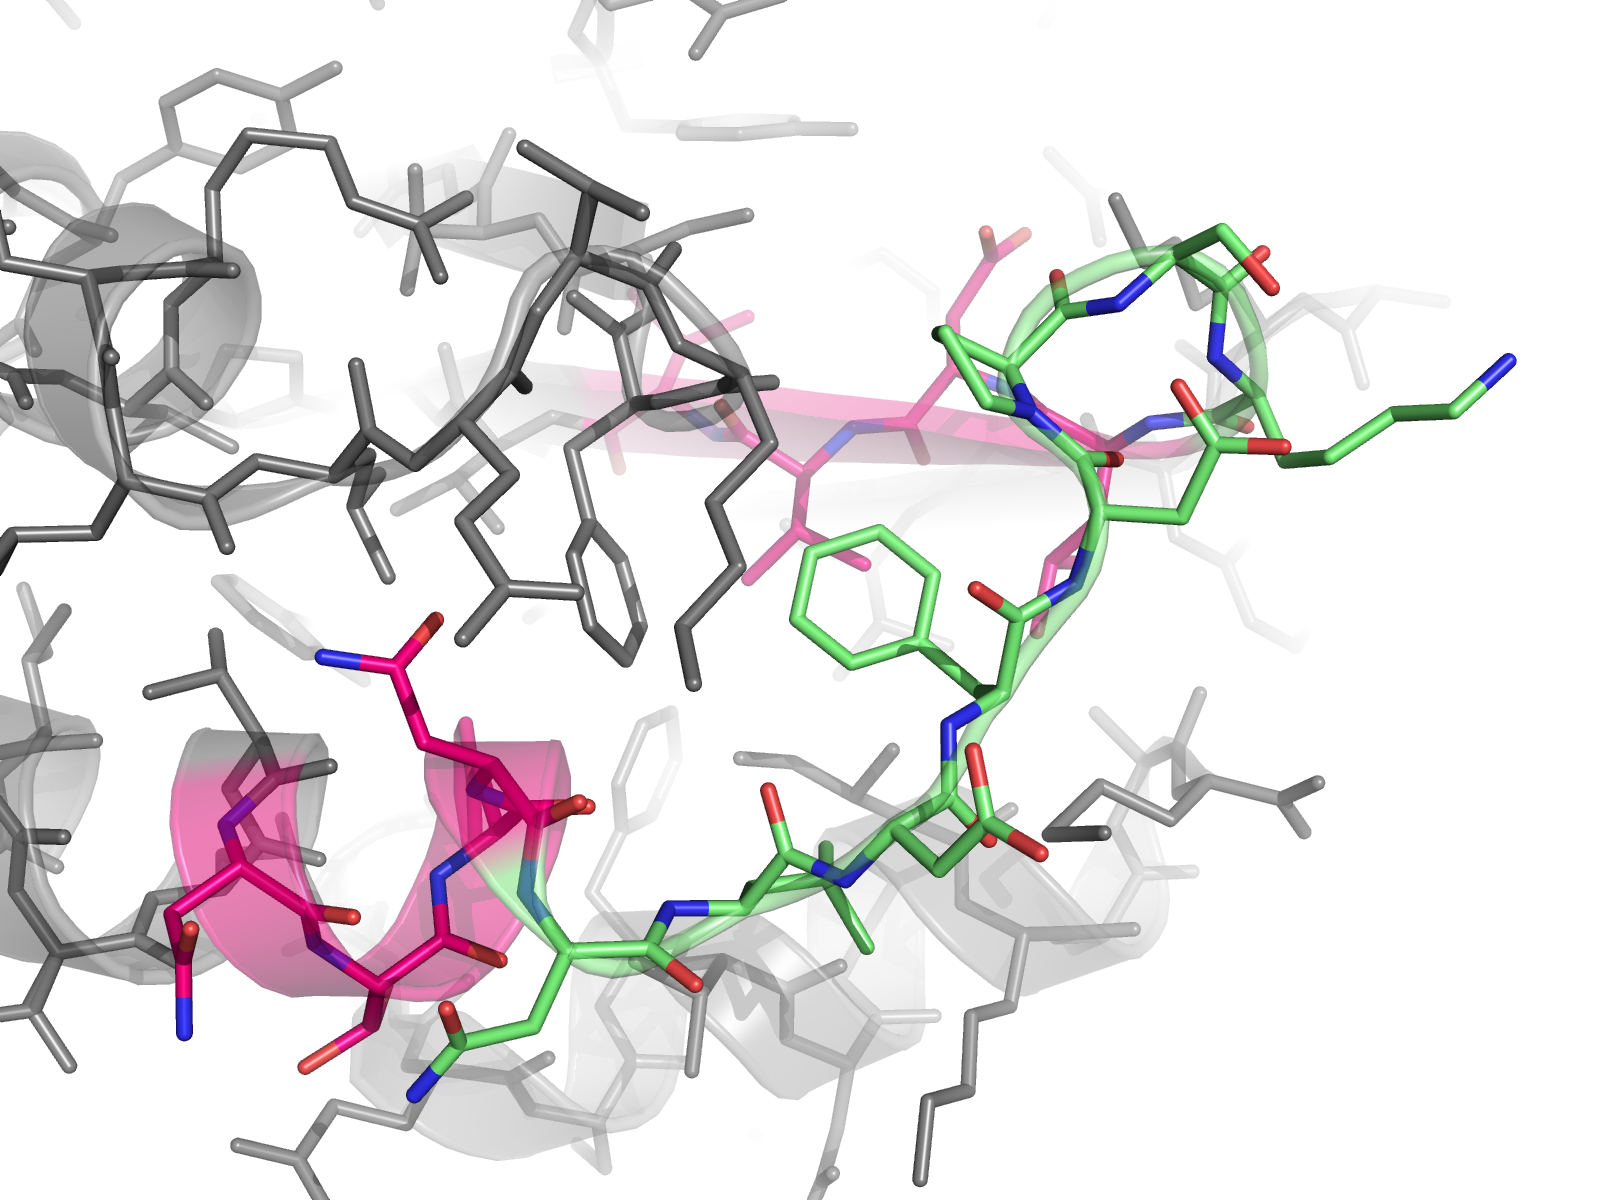
\includegraphics[width=1.0\textwidth]{04-Database/allowed/strand-helix.png}
            }}
            
           
            \subfigure[A typical loop formed within a distorted super-secondary structure motif. \mer{8} loop in 1OOEA from residue 35.]{\scalebox{0.54}{
            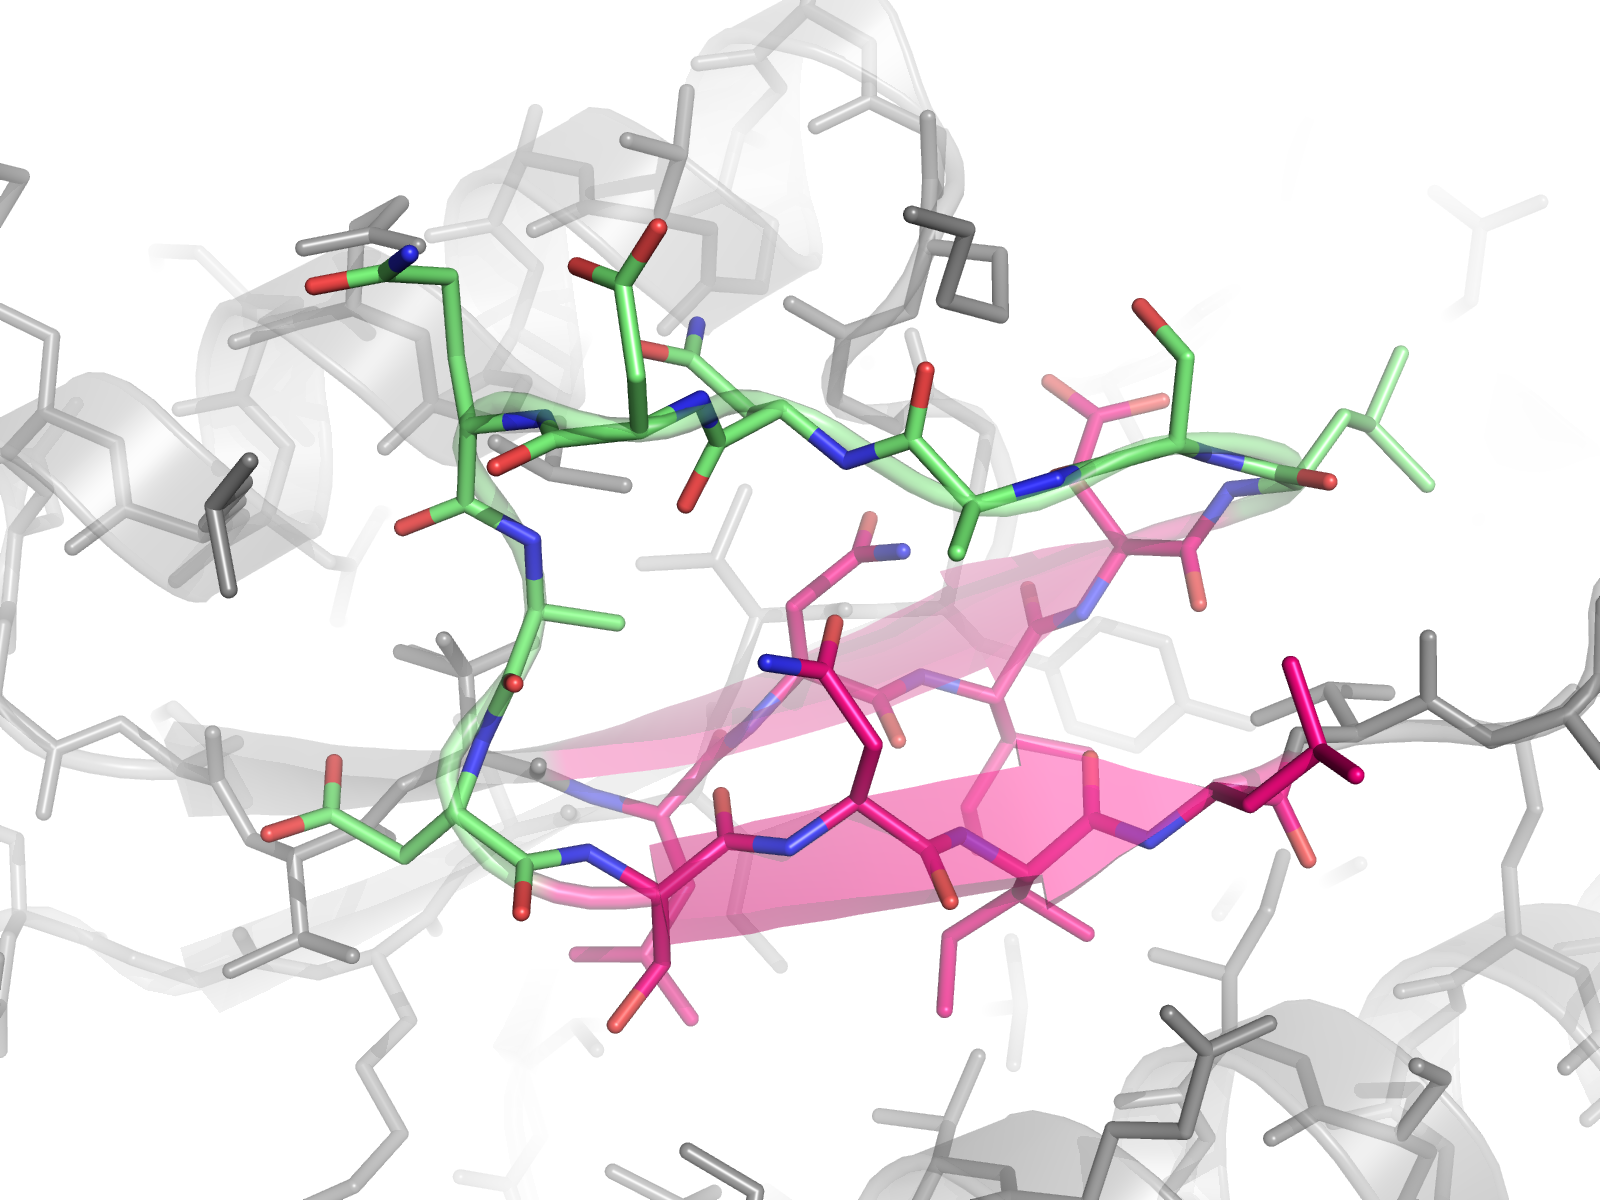
\includegraphics[width=1.0\textwidth]{04-Database/allowed/surface.png}
            }}
            
            \subfigure[A typical compound loop. \mer{8} loop in 1PFBA from residue 48.]{\scalebox{0.54}{
            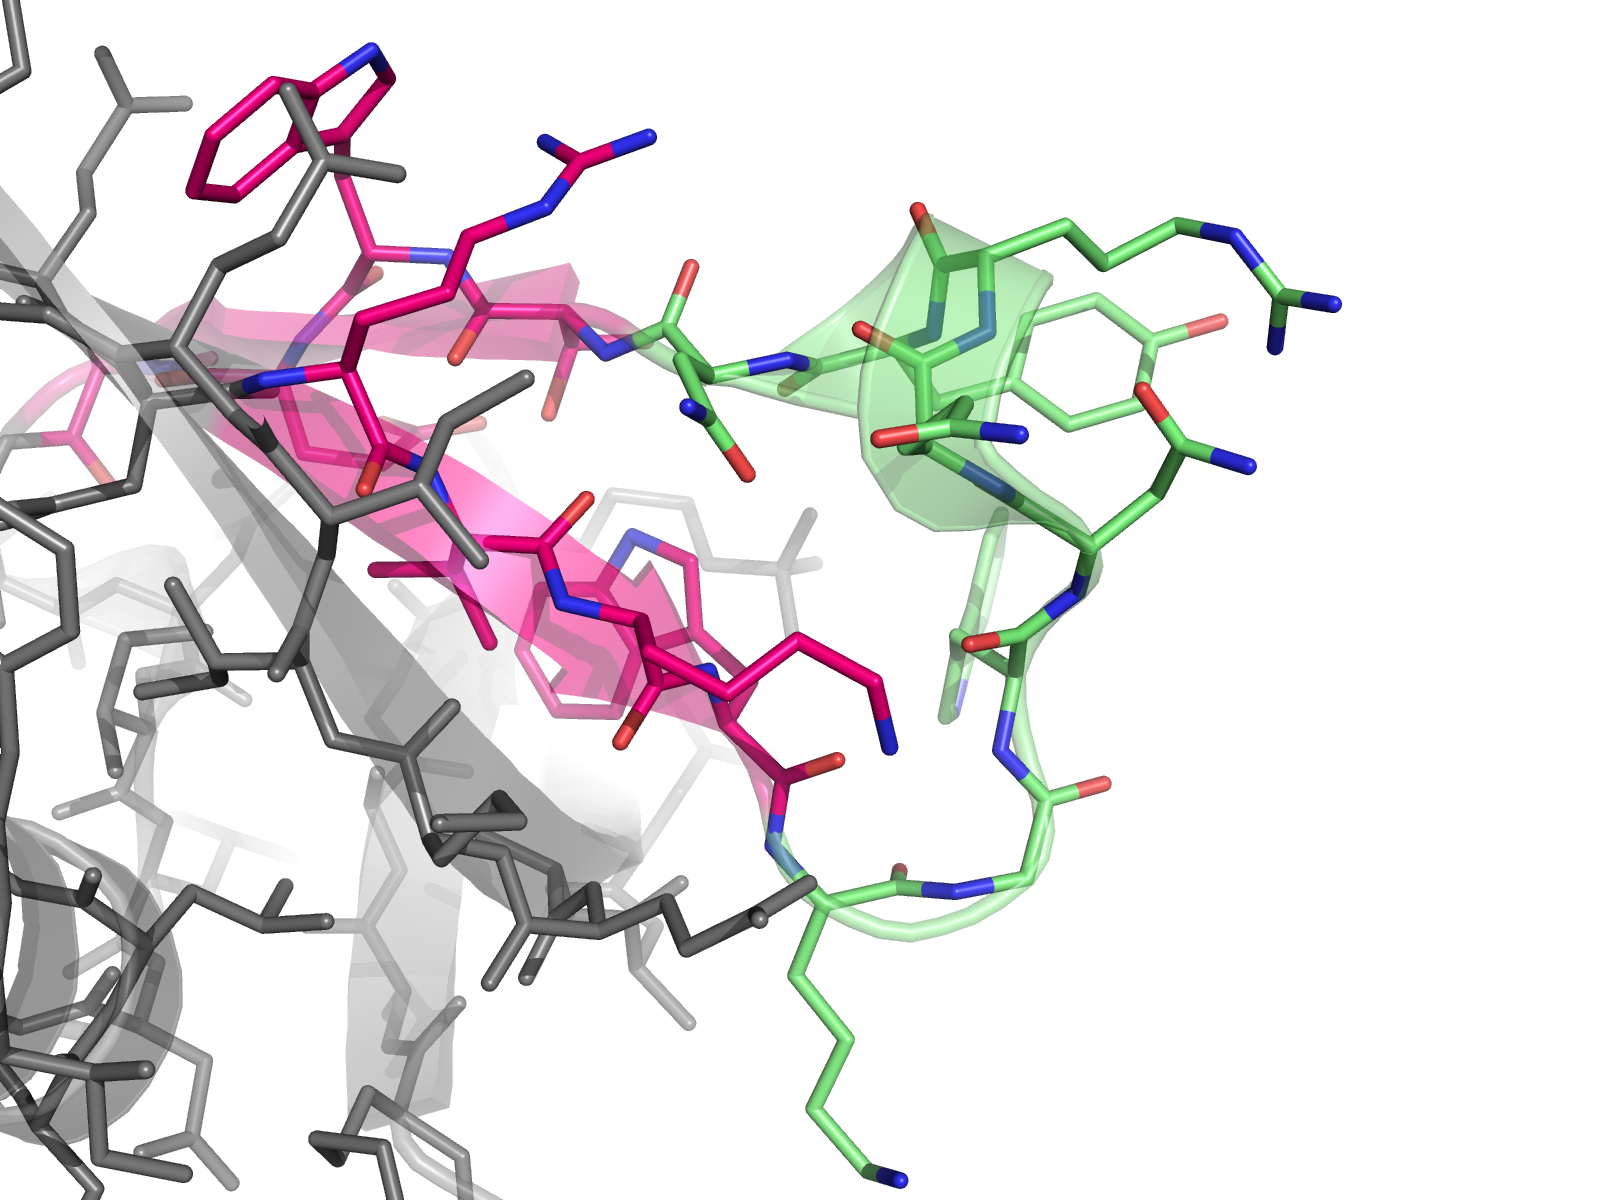
\includegraphics[width=1.0\textwidth]{04-Database/allowed/compound.png}
            }}
 
\caption[Typical medium to long range loops]{Typical medium to long length loops. 8-mers were chosen to illustrate the gross structural trends found
in this approximate size of  loop.
The loop and secondary structure anchors are shown in green and magenta respectively.
Images created with \pymolV.}

\label{fig:db:typicalloops}

\end{center}
\end{figure}







Importantly, table \ref{table:db:disallowedloop} shows that for longer loops the fraction 
of loops containing residues within
the disallowed regions of Ramachandran space increases several fold. Examples
of such loops are shown in figure \ref{fig:db:disallowedloop}. The fact that
up to 13.5\% of medium to long length loops have residues which populate these
regions of Ramachandran space (table \ref{table:db:disallowedloop}) has implications for the process of modelling
loops, specifically the scope of the conformational search.



\begin{table}[hp]
\begin{center}
\begin{tabular}{+c^c^c^c^c^c^c^c}
\toprule
  \multicolumn{2}{c}{\textbf{Loop}} & \multicolumn{6}{c}{\textbf{\% with Disallowed Angle}}\\

\rowstyle{\bfseries}
Length & Count  & I     & II    & III   & IV    & V    &  Any  \\
  
   \midrule
   0   &  321   &  0.0  &  0.0  &  0.0  &  0.0  &  0.0 &  0.0  \\
   1   &  930   &  0.4  &  3.1  &  0.2  &  0.1  &  0.0 &  3.9  \\
   2   &  2116  &  0.6  &  2.8  &  0.4  &  0.0  &  0.0 &  4.0  \\
   3   &  1817  &  1.8  &  0.8  &  0.6  &  0.0  &  0.1 &  3.2  \\
   4   &  2001  &  0.7  &  0.3  &  0.7  &  0.0  &  0.0 &  1.8  \\
   5   &  1730  &  1.9  &  1.1  &  0.7  &  0.6  &  0.1 &  4.3  \\
   \midrule
   6   &  1140  &  1.6  &  1.7  &  0.6  &  0.4  &  0.2 &  4.3  \\
   7   &  895   &  1.6  &  1.0  &  0.8  &  0.3  &  0.1 &  3.8  \\
   8   &  683   &  2.9  &  1.8  &  1.3  &  0.0  &  0.0 &  6.0  \\
   9   &  565   &  2.8  &  1.6  &  0.4  &  0.2  &  0.0 &  5.0  \\
   10  &  488   &  2.3  &  2.5  &  2.3  &  0.2  &  0.0 &  7.0  \\
   11  &  412   &  5.3  &  2.7  &  1.2  &  0.7  &  0.5 &  10.2 \\
   12  &  296   &  6.8  &  4.1  &  3.0  &  0.3  &  0.7 &  13.5 \\
   \midrule
   13  &  213   &  3.3  &  3.8  &  1.9  &  1.4  &  0.5 &  10.3 \\
   14  &  220   &  3.2  &  1.4  &  1.4  &  0.0  &  0.0 &  5.9  \\
   15  &  158   &  3.8  &  1.3  &  1.9  &  0.6  &  0.0 &  7.6  \\
   16  &  117   &  3.4  &  1.7  &  0.9  &  1.7  &  0.0 &  7.7  \\
   17  &  98    &  7.1  &  3.1  &  0.0  &  0.0  &  0.0 &  10.2 \\
   18  &  103   &  3.9  &  1.0  &  1.0  &  0.0  &  0.0 &  5.8  \\
   19  &  95    &  6.3  &  2.1  &  3.2  &  0.0  &  0.0 &  11.6 \\
   20  &  62    &  4.8  &  1.6  &  0.0  &  0.0  &  1.6 &  8.1  \\

\bottomrule
\end{tabular}
\caption[Loops containing residues in the disallowed Ramachandran regions.]{Loops containing residues in the disallowed Ramachandran regions. N.B. a zero length loop refers to a \ahelix\ directly joined to a \bstrand\ or visa-versa.}
\label{table:db:disallowedloop}
\end{center}
\end{table}





\begin{figure}[hptb]
  \begin{center}
  
    \mbox{  
    
            \subfigure[Ramachandran plot showing the five disallowed regions\cite{NATIVE:DISALLOWED}.]{\vspace{0.5cm}\scalebox{0.47}{
            \includegraphics[width=0.884\textwidth]{04-Database/disallowed/disallowed.png}
            }}
            
            \quad
  
            \subfigure[Region I: A \mer{8} loop in 1SNNA from residue 21. Disallowed residue Lys-25 is stabilised by a close salt-bridge interaction.]{\scalebox{0.47}{
            \includegraphics[width=0.884\textwidth]{04-Database/disallowed/region_1.png}
            }}
            
    } \mbox{ 
            
            \subfigure[Region II: A \mer{8} loop in 1JHJA from residue 83. A compound loop composed of a \be-turn and a very short helical region. Like in typical type II' beta turns, disallowed \mbox{Glu-87} is stabilised by an \mainchain\ \mbox{hydrogen bonding} interaction.]{\scalebox{0.47}{
            \includegraphics[width=0.884\textwidth]{04-Database/disallowed/region_2.png}
            }}
    
            \quad
    
            \subfigure[Region III: A \mer{8} loop in 1LZLA from residue 203. A particularly compact loop, where disallowed Leu-208 is packed tightly into the protein core.]{\scalebox{0.47}{
            \includegraphics[width=0.884\textwidth]{04-Database/disallowed/region_3.png}
            }}
            
    } \mbox{
        
            \subfigure[Region IV: A \mer{7} loop in 2PTH\_ from residue 64. A compound loop involving a short helical region.]{\scalebox{0.47}{
            \includegraphics[width=0.884\textwidth]{04-Database/disallowed/region_4.png}
            }} 
    
            \quad
    
            \subfigure[Region V: A \mer{7} particularly extended loop in 1O6DA from residue 119. In this case, Ser-120 is stabilised by a \sidechain$\to$\mainchain\ hydrogen bond.]{\scalebox{0.47}{
            \includegraphics[width=0.884\textwidth]{04-Database/disallowed/region_5.png}
            }}}%
\caption[Loops with residues occupying disallowed regions of Ramachandran
    space]{Loops with residues occupying disallowed regions of Ramachandran
    space. For all images the disallowed residue, loop and anchor residues
    are in yellow, green and magenta respectively. Images created with \pymolV.}%
\label{fig:db:disallowedloop}
    
  \end{center}
\end{figure}







\subsection{Final Comments}

\subsubsection{Previous Loop Test Sets}

The most common benchmarks used in previous individual loop modelling calibrations are the test sets from Xiang et al.\cite{METHOD:Xia2002} and Fiser et al.\cite{METHOD:Fis2000}. These sets both used structures of $<$2.0\AA\ resolution,  a pairwise sequence identity cutoff of 20\% and 60\% respectively and contain loops of length 5$\to$12 and
1$\to$14 residues respectively. Fiser et al. chose 40 loops at random of each length with no more than one from each original PDB structure. By contrast Xiang et al. used all loops present within their smaller \dataset\ which contained 135 proteins derived from CulledPDB. The loop definitions used by these studies are similar to the definition developed during this work in that \dssp\ was used to define loop
boundaries. By contrast however, Fiser defines no prescribed lower limit on secondary structure length and Xiang uses any secondary structure annotation instead of only `H' and `E'.

 
It has been noted that the \mer{11} and \mer{12} residue loops in the Fiser \testset\ contain a high degree of secondary structure from the protein core\cite{METHOD:Plop},
although it is unclear why these would not have been filtered by their criteria. In any case these structures are inherently more appropriate for comprehensive building algorithms that utilise knowledge of either \ahelix\ packing or \bsheet\ strand register to build elements of the protein core. They are, therefore, less appropriate to loop modelling as bulk secondary structure prediction is not  required in high sequence-identity comparative modelling. As the loop selection definition
used in this work is derived from strict secondary structure annotation, such concerns are removed. Only very short regions of secondary structure remain, which should lie within the attainable scope of any viable loop modelling methodology.



The largest structural test set used in a method calibration prior to this study was 833 loops ranging from 4 to 12 residues in length\cite{METHOD:Plop}. In comparison to this, this study uses a database of unprecedented size, using all loops of between 6 and 11 residues in length, from the set of 2,349 extremely high-resolution structures described in section \ref{chapter:database:protein}. The exact counts are shown in table \ref{table:db:exactloopcount}. The software can generate loops of any user-defined length, however, the upper limit of 11 residues was chosen to in this work limit the duration of 
simulations with such a large test set and limited computational resources.
 Methods such as \plop\cite{METHOD:Plop} specify that on a 1.4\ghz\ AMD based PC, the maximum time for a \mer{12}
 was 160 hours. Even with more powerful processors available now, performing this test on the 4,183 test loops is unrealistic with current computational resources.


\begin{table}[hbtp]
\begin{center}
\begin{tabular}{+c^c}
\toprule
\rowstyle{\bfseries}
  Length & Count \\
\midrule
6     &  1,140 \\
7     &  895 \\
8     &  683 \\
9     &  565 \\
10    &  488 \\
11    &  412 \\
\midrule
Total &  4,183 \\
\bottomrule
\end{tabular}
\caption{Exact counts for the chosen range of loops derived for this work.}
\label{table:db:exactloopcount}
\end{center}
\end{table}


\subsubsection{The Chosen Loop Definition}

Within the loop definition chosen for this work, it is possible to obtain short sections of secondary structure within longer compound loops. These could be for example a short \ahelix\ packed against the protein surface or a short additional \bstrand\ in hydrogen bonding contact with a \be-sheet. Within a given set of structural templates, longer regions of secondary structure are very likely to be structurally conserved and possess a strong sequence signal. These would, therefore, be included as part of the rigid body in standard comparative
modelling studies. The converse is true of short secondary structure.


In light of this, it is assumed
that the loop definition used in this work is compatible with the types of loop found in comparative modelling tasks and will therefore result in a fair test set. Of course, some particularly long regions will be also found, however derived statistics obtained from the analysis of these irregular regions will nonetheless remain valid. Calibration of loop modelling can be performed on a subset of these loops of a range of suitable lengths. 




\section{Summary}
In summary, PDB culling servers were compared to find the most suitable for use in this study. \textsc{Pisces} was chosen because of its continuing support, regular updates, and enhanced feature set. \pdbdb, which utilises
the \uobf, was used to post-screen this \basechainlist. The relevant PDB files were downloaded, parsed, modified, filtered, rebuilt and then energy minimised
using \pd. This final \jsubset\
of 2,349 PDB files and complementary \dssp\ files will be referred to at \thothdb.

 From \thothdb, using the structural annotation output of \dssp\ as the basis for the loop definition,\ a representative set of medium to long length loops was defined for use in this study. Any loop database derived on-the-fly
will be referred to as \thothloopdb. Unless otherwise stated, the loops contained within
\thothloopdb\ are defined exclusively by the filtered structures in \thothdb\ and the
loop definition provided in \mbox{section \ref{section:loopcriterion}}.
         %  4. Development of the PDB databases
\chapter{Development of a Reduced-Complexity Protein Representation and Coarse-Grained Build Strategy}
\label{chapter:reduced_rep}


\begin{quote}
``I have opinions of my own -- strong opinions -- but I don't always agree with them.'' \\
--- \textit{George Bush}
\end{quote}

\section{Introduction}

As has been discussed, the structure of globular proteins can be conceptually divided into regions of regular secondary structure, mainly \ahelixs\ and \bstrands, termed the protein-core and  loop-structures which connect them. The prediction of these loops remains the most taxing element of comparative modelling, largely due to the lack of homology information in the template structures for these regions. Generally, other than the primary sequence, the only information available to the modelling process is the location at which the loop enters and leaves the protein core. The conformational space, of loops greater in length than around seven residues, is not well represented by available PDB\ fragments. The structure of these longer loops must, therefore, be modelled using non-comparative methodologies.


The overall aim for this chapter is to describe the development of a torsional reduced-representation, coupled to a rapid method  for the enumeration  of conformational states and a complementary structural filtering procedure. The output of such a build-method is a list of   defined torsional states, which represent the available coarse-grained conformational space. This is an ideal foundation for a hierarchical torsional-refinement procedure, as large regions of conformational space may be eliminated from the more computationally costly refinement process. The development of the refinement levels is described in chapter \ref{chapter:prearcus}.
\section{Reducing Complexity}
\label{section:complexity}

The idea behind reduced protein representations has already been partially discussed in section \ref{section:protein_rep}. Studies have also been performed which look at the applications for reduced state models\cite{METHOD:Kol2004,METHOD:Sko98}. The central concept is that conformational space can be reduced to a large extent, without compromising the detail of the protein model. The reduction should be planned carefully to ensure that its ability to represent the native state is not  fundamentally impaired.
 
 When designing a reduced-representation a number of key choices are made. The first is the atomic representation, the second is how space will be described, third is the energy function that will discriminate between the states and finally some form of sampling mechanism must be chosen. The majority of reduced models utilise a much lower number of particles than would be contained within an all-atom model, for example using single-particle centroids positioned along the \ca$\to$\cb\ vector to represent the \sidechain\ atoms\cite{COMPCHEM:Gib2001}. The exact definition of the \forcefield\ is tightly-coupled to the chosen protein representation, because the shape of the energy wells has to take any simplified-geometry into account. 

Many different method developments have explored the discretisation of conformational space. Several have attempted to use lattice models, which simplify Cartesian space using discretised coordinate systems, at least for the \mainchain\ atoms in the model.  These lattice definitions include tetrahedral lattices\cite{COMPCHEM:Hin92},  extended face-centred cubic lattices\cite{METHOD:Cov90} and ``knights-walk'' lattices\cite{METHOD:Sko93}, with conformation counts of \mbox{$3^{n/2}-3$}, \mbox{$41^{n-3}$} and \mbox{$55^{n-3}$} respectively. At the crudest cubic-grid level, the representation is relatively poor, however, non-cubic fine-grid systems have been shown to approximate the native state of a protein to near-atomic accuracy\cite{METHOD:Kol2003}. Other methods, use continuous-space models with reduced degrees of freedom, for example some have used optimised limited sets of backbone torsion angles to represent the path of the protein chain\cite{COMPCHEM:Gib2001,COMPCHEM:Rooman91}. 

The central question is, how detailed does a reduced conformational representation need to be in order to represent the native conformation with sufficient accuracy? The results from a previous study \cite{METHOD:ParkLevitt}, which analysed the relationship between model-complexity and the accuracy of structural description, are shown in figure \ref{fig:reducedrep:complexity}. 

\begin{figure}[hbtp]
\begin{center}
\includegraphics[width=0.85\textwidth]{./05-ReducedRep/complexity/complexity.pdf}
\caption[The relationship between model-complexity
and structural-representation]{The relationship between model-complexity
and structural-representation.\\
A fit is shown to a second-order exponential decay. Two representations are highlighted, which out-perform
the other methods in terms of finding an optimal balance between complexity and representation. These are the optimised torsional representations of Rooman et al.\cite{COMPCHEM:Rooman91}
and Park et al.\cite{METHOD:ParkLevitt} shown in red and green respectively.
(Data\cite{METHOD:ParkLevitt}.)}
\label{fig:reducedrep:complexity}
\end{center}
\end{figure}

Two broad trends are clear; The first is that as complexity increases, the quality of the representation
quickly plateaus to a cRMS of around 1.0\AA, signifying that overly-complex reduced representations yield no appreciable additional benefit. The second trend is that the representations which strike the best balance  are optimised torsional models. Further development of such a torsional representation is considered in this work, continuing from the published method 
\raft\cite{COMPCHEM:Gib2001}.
    
  
\section{The History of RAFT}

\raft\cite{COMPCHEM:Gib2001}, or Reduced Angle Forcefield for Tertiary structure prediction, was originally developed at the \uob,\ for application to \abinitio\ structure prediction of small protein molecules. The basic philosophy behind this implementation was to vastly reduce the scale of conformational space, by modelling the protein backbone with a limited set of residue-specific torsion-angle pairs, derived from PDB data.
As has been discussed, the reason that the conformational space of peptides can be reduced, is that the Ramachandran plot is limited to certain discrete areas of torsional space and reasonably compact in distribution. 

Six, residue-dependent \phipsi\ angle-pairs in three Ramachandran regions were allocated in the original \raft\ study. Two were defined to be typical $\alpha$-helical angles, three \bstrand\ angles and finally a single left-handed helical angle. 
For a given peptide, a series of these identifiers of the same length is termed a \emph{conformer}, which completely defines a given backbone conformation within the reduced set. The reduced \angleset\ was developed in combination with a simplified reduced-particle  forcefield for rapid energy evaluation of potential structures. 
Figure \ref{fig:reducedrep:raft_conformers} shows that, within this approximation, the ability to fold the native state is very reasonable for peptide fragments -- each example shown is proposed to be a small independent folding unit\cite{COMPCHEM:Ped1997}. 



\begin{figure}[hbtp]
\begin{center}
\includegraphics[width=0.67\textwidth]{05-ReducedRep/complexity/conformer.png}
\end{center}
\caption[Example \raft\ conformers]{Example \raft\ predictions. Each native peptide is proposed to be an independent folding-unit\cite{COMPCHEM:Ped1997}. The crystal-fragment and predicted structures are shown in black and grey respectively. The PDBID, residue range and \ca-cRMS appear below each image. Image adapted from\cite{COMPCHEM:Gib2001}.}
\label{fig:reducedrep:raft_conformers}
\end{figure}



\section{Six-state Loop-Modelling is Non-Trivial}

Modelling the conformation of a short surface loop may seem like an insignificant task, however, the difficulty becomes evident when the number of possible conformations which can be adopted is considered.  Assuming just six particular states and ignoring the conformational freedom of any \sidechains\, the exhaustive search on a \mer{12} loop yields 6\superscript{12} possible conformations -- \ie\ 2,176,782,336 structures in total. 

Of course, the majority of these conformers will not satisfy the restraints of entering and leaving the protein core at the correct locations and in the correct orientation. A significant proportion will also sterically clash with either themselves or with the protein surface. These facts are, however, not known from the outset and therefore building and subsequent evaluation of these conformations must be performed, before they can be eliminated from the search process. 

Following on from this idea, it is clear that full energetic evaluation of all potential loop structures would be hugely wasteful. Merely a 5 second building process and energy evaluation on each of these structures, for just one loop, would take a total of over 345 years. It is, therefore, clear that some sort of rapid culling of large numbers of conformations  is required, followed by effective sampling of the surrounding conformational space.

This process of culling potential loop structures can be relatively easily vocalised - simple statements like ``remove clashing conformations'' are easy to say - however the technical details of how one would efficiently perform this computationally is more complex. The computational practicality of storing coordinates for all these possible conformations or re-deriving the coordinates at every step is barely feasible -- just marking the viability of all conformations true or false for a given \mer{12} conformation in memory, each requiring just 1 bit, which would require 260\mb\ of storage; storing the energy would require 8.11\gb. Even at this level of storage, the need to convert valid bit-positions back into their conformers is ignored, but is required to facilitate sorting and subsequent re-evaluation under more complex calculations.
All-in-all, this describes the need for careful design of the computational method behind any build process to ensure tractability of the calculation.   



\section{Ramachandran Distributions}

Firstly, it is important to discuss the gross population distribution changes which occur when loop regions are considered in isolation. Three types of Ramachandran plot are shown in figure \ref{fig:reducedrep:ramachandran} to illustrate the different aspects. Glycine and proline are excluded from these plots due to large differences in their distributions and are discussed separately later in this chapter.

\begin{figure}[hbtp]
  \begin{center}
    \mbox{
      \subfigure[All structure scatter\superscript{1}]{\scalebox{0.42}{\includegraphics[width=1.0\textwidth]{05-ReducedRep/ram_plot/NotGlyOrPro_All_B_Scatter.png}}} \quad
      \subfigure[Loop structure scatter\superscript{2}]{\scalebox{0.42}{\includegraphics[width=1.0\textwidth]{05-ReducedRep/ram_plot/NotGlyOrPro_Loop_B_Scatter.png}}}
      }
      \vspace{0.5cm}
    \mbox{
      \subfigure[All structure 3D landscape\superscript{1}]{\scalebox{0.42}{\includegraphics[width=1.0\textwidth]{05-ReducedRep/ram_plot/NotGlyOrPro_All_B_Contour3D.pdf}}} \quad
      \subfigure[Loop structure 3D landscape\superscript{2}]{\scalebox{0.42}{\includegraphics[width=1.0\textwidth]{05-ReducedRep/ram_plot/NotGlyOrPro_Loop_B_Contour3D.pdf}}}       }
      \vspace{0.5cm}
    \mbox{
      \subfigure[All structure contour\superscript{1}]{\scalebox{0.42}{\includegraphics[width=1.0\textwidth]{05-ReducedRep/ram_plot/NotGlyOrPro_All_B_ContourHiRes.pdf}}} \quad
      \subfigure[Loop structure contour\superscript{2}]{\scalebox{0.42}{\includegraphics[width=1.0\textwidth]{05-ReducedRep/ram_plot/NotGlyOrPro_Loop_B_ContourHiRes.pdf}}}       }
\caption[Ramachanran distribution changes in loop regions]%
{Ramachandran distribution changes in loop regions. Data derived from all residue types except glycine and proline. Data\superscript{1}: 348,915 occurrences (87.74\%) in all structural classes. Data\superscript{2}: 130,147 occurrences (80.22\%) in loop structure only.}
    \label{fig:reducedrep:ramachandran}
  \end{center}
\end{figure}

The overall Ramachandran plot distribution remains unchanged when loop-structure is considered in isolation. This is to be expected, as the occupied regions of the Ramachandran plot are determined predominantly by steric interactions. Figure \ref{fig:reducedrep:ramachandran}-a, however, does show that the central density of the highly populated regions thins when only loops are considered, leaving proportionally more scattered data. From figure \ref{fig:reducedrep:ramachandran}-b it can be seen that the $\alpha$-region in globular protein structure is hugely favoured, reducing dramatically in loop regions as the helical bias is less pronounced. The change is shown quantitatively in figure \ref{fig:reduced_rep:propensity_change}.
Finally, in figure \ref{fig:reducedrep:ramachandran}-c it can be seen that the gross distribution within both the \al\ and \be-regions alters when loop regions are isolated.
When the \be-region for all structural data is considered, the population centred around  \mbox{$\Phi=$ -139, $\Psi=$ 135} is due to anti-parallel \bsheet. Evidently, the regularity of the anti-parallel \bsheet\ imposes conformational restrictions which are not present in loop structure, as there is a shift towards $\Phi=$ -70 in this case.

\begin{sidewaysfigure}[hptb]
\begin{center}
\subfigure[Angle-pair indices]{\scalebox{0.32}%
{
\includegraphics[width=1.0\textwidth]{05-ReducedRep/propensity/ramachandran.png} }}\qquad\subfigure[Comparing the \raft, all-structure and loop-structure \anglesets]{\scalebox{0.6}%
{\includegraphics[width=1.0\textwidth]{05-ReducedRep/propensity/propensity.pdf}}}
\end{center}
\caption{Propensity changes between different structural classifications; when using six parametised angles.}
\label{fig:reduced_rep:propensity_change}
\end{sidewaysfigure}

\section{Structural Considerations}

We have described that the original \raft\ \angleset\ shows promise for small proteins and therefore, as the overall Ramachandran distribution does not change for loop regions, should be applicable to loop-modelling. We have, however, also shown that there is significant change in the relative distribution between Ramachandran regions when loops are considered in isolation. This implies that re-fitting should be performed to assess changes in optimal angle placement for loop regions, analyse whether more angles per-residue are required to account for increased variability and to measure the propensity for each angle-state.

\subsection{Glycine and Proline}

It is especially important to represent glycine and proline correctly in this study because they are more prevalent in loop regions by 157.5\% and 161.7\% respectively (table \ref{table:database:propensity}).
Due to the lack of \sidechain, glycine is less sterically hindered and can therefore routinely adopt backbone torsional angles that the other residues cannot. The six selected angles are therefore more diffuse in order to cover the required extra conformational space. A second special case, proline, is more conformationally restrained due to the fact that the \sidechain\ covalently bonds back onto its amino-group. This means that its $\Phi$-angle is largely inflexible resulting in a reduction in conformational diversity. Proline was originally fitted to two distributions on the Ramachandran map corresponding to the two predominant populations of the $\Psi$-angle. Specific aspects for both these residues are discussed as appropriate below.

\subsection{Backbone Stereochemistry}

Figure \ref{fig:intro:bb_torsion} was previously used to show that the protein \mainchain\ can be effectively described by three torsions per residue.
Relative occurrences of the cis and trans-peptide conformations were calculated during this work and are shown in  table \ref{table:intro:cis_occurence}. 
\begin{table}[htbp]
\begin{center}
\begin{tabular}{+l^r^r^r}
\toprule
\rowstyle{\bfseries} Type    &    Trans &  Cis  & \% Cis \\
\midrule
Proline &   32,591 & 1,960 &  5.67\% \\
Other  &   705,014 &   305 &  0.04\% \\
\bottomrule
\end{tabular}
\caption{Occurrences of the cis-peptide group conformation.}
\label{table:intro:cis_occurence}
\end{center}
\end{table}

Figure \ref{fig:reducedrep:omg}
shows that the conformational freedom of the  \Omg-torsion
is highly restricted in nature. Due to this 
inflexibility, the \Omg-torsion is commonly neglected in many modelling methods, treated exclusively as the trans-state. Compared to other residues, however, the \Omg-torsion of proline is an important consideration for modelling due to its  vastly increased occurrence as a  cis-peptide. In fact, the vast majority of cis-proline residues can be attributed to loop-structure in general. Due to this importance, the cis-state of proline is defined within the model used for this dissertation, but treated as a constant of either 180\degree\ or 0\degree\ for the build process alone. All other residues are treated as though they are in the trans-conformation.

\begin{figure}[htbp]
  \begin{center}
    \mbox{
      \subfigure[All Residues Except Proline]{
      \scalebox{0.45}{
      \includegraphics[width=1.0\textwidth]{05-ReducedRep/cis/omega_dist_allNoPro.pdf}}} \quad
      \subfigure[Proline]{
      \scalebox{0.45}{
      \includegraphics[width=1.0\textwidth]{05-ReducedRep/cis/omega_dist_proonly.pdf}}}
      }
    \caption{The distribution of the \Omg\ main-chain torsion.}
    \label{fig:reducedrep:omg}
  \end{center}
\end{figure}

It is noted that the remaining 305 non-proline cis-peptide occurrences are  highly important in the active sites of proteins and are, therefore, crucial to function. The neglect of the cis-state fundamentally means that the method developed in this work would  fail for these very rare specific cases. Such \Omg-angles could be enabled for short loops known to be part of an active-site, however, their general use is not feasible in terms of typical surface loop prediction. This is  both because the number of possible conformations is vastly increased and because the conformational search itself is polluted by large numbers of highly-improbable competing energy minima.


\subsection{Conformational Freedom vs. Angle-pair Count}

Figure \ref{fig:reducedrep:angle_coverage} shows that individual residue types are represented to different accuracies by six residue-states.
 In contrast to the original \raft\ study, which used six angles for every residue type, there is no reason why the number of angles cannot be varied on a per-residue basis. 
\begin{figure}[hbtp]
\begin{center}
\includegraphics[width=0.7\textwidth]{05-ReducedRep/closest_angle/closest.pdf}
\caption[The data coverage of the original \raft\ \angleset.]{The data coverage of the original \raft\ \angleset. To obtain this plot, the relevant Ramachandran scatter-plot  is loaded per residue-type, with the matching representative \raft\ angle-pairs superimposed. Around each angle-pair, a circle is drawn. The radius of each circle is gradually increased and the percentage of data within all circles is measured at each increase. This radius is termed the radius of influence. In real terms this radius equates to the search radius which must be employed to generate the exact native loop conformation for a given percentage of native loops -- obtained via optimal torsional perturbations of \emph{up to} that magnitude.}
\label{fig:reducedrep:angle_coverage}
\end{center}
\end{figure}

A second aspect is one of implementation. Proline only required four parametised angles in the original \raft\ work, however it was given six angles purely to aid implementation of the software; Due to enhanced memory management of more modern software development platforms, shortcuts like this are no longer required. 

There are multiple cases which may need additional angles; serine occurs most regularly in the disallowed regions of the Ramachandran plot, glycine shows a vastly increased conformational spread and asparagine fits relatively poorly to  six residue-states.
Having specified a possible  need for additional angles when modelling loop regions, it should be emphasised that the converse argument is also true -- \ie although one could add many additional angles to give a fine-grained definition of conformational space, the huge problem of the ``conformational explosion'' must always be considered. For example, when exhaustively  enumerating the conformer for a typical \mer{12} fragment, increasing from a six-state \angleset\ to a seven-state \angleset\ yields 6.3$\times$ more conformers. Alternatively, by increasing to an eight-state \angleset, an increase of 31.6$\times$ occurs. This obviously increases a 1 day calculation to a 1 week and 1 month calculation respectively. This is not a cheap price to pay, especially when method calibration and parametisation is required and computational resources are limited. It should be remembered however that, as described in section \ref{section:complexity}, some modern lattice methods use conformational spaces which scale with $41^{n-3}$ or $55^{n-3}$, far in excess of the $6n$ of the original \raft\ study.


\subsection{Subsequent Refinement}
\label{section:reduced_rep:subsequentrefinement}

Figure \ref{fig:reducedrep:searchradius} shows that, under the original \raft\ angle-pair definitions, with respect to a second-stage torsional perturbation remodelling method, a 60\degree\ maximal perturbation would yield excellent data coverage.
One small caveat is that,
even perturbations of up to 120\degree\ would not cover the data within disallowed clusters II and III. These clusters are important for the $i+1$ position of some types of $\beta$-turn, as previously shown together to be important in up to 7\% of loops in table \ref{table:db:disallowedloop}. However, a search radius of 120\degree\ would not be computationally tractable in  later refinement stages.
As serine is known to occupy these regions with significant frequency, there is an argument for re-parametisation of this residue and possibly more fitted angle-pairs. It would be hoped that any automatic re-parametisation of angle-pairs for surface loop modelling would yield coverage of these regions for serine. 

\begin{figure}[hbtp]
\begin{center}
\includegraphics[width=0.55\textwidth]{05-ReducedRep/ram_plot/NotGlyOrPro_All_B_Scatter.png}
\includegraphics[width=0.95\textwidth]{05-ReducedRep/search/radius.png}
\caption[Torsional Search Radius]{%
Torsional search-radius.
An arbitrary set of six \raft\ angle-pairs are shown as stars, with $\pm$180\degree\ Ramachandran plot boundaries shown as red dashed lines. From left to right the radii of influence around the idealised angles are shown at 60\degree, 90\degree\ and 120\degree\ respectively.}
\label{fig:reducedrep:searchradius}
\end{center}
\end{figure}


\section{The Angle-fitting Method}

The fitting method in the original \raft\ study, was based on a 2D search of the Ramachandran plot, in order to minimise the total distance of all the data points to their nearest parametised angle. This essentially results in the representative angles being assigned to the most densely populated regions of the Ramachandran map. The scoring method has been kept in this study with one change, outlined below.

The fitting procedure was performed for each residue-type in isolation. Due to computational limitations, the original study used a course 1.0\degree\ grid, restricted to each of the three most populated Ramachandran regions. Following an exhaustive search over the three independent grids, a search using a smaller, finer 0.2\degree\ grid was performed for each allocated angle in turn. The solution obtained was the optimum for a given grid definition, however, intrinsically dependent on the arbitrary rectangular 2D boundaries chosen by the user. 

 An alternative procedure was chosen for this work as a scheme of random perturbations followed by the \emph{simultaneous} score minimisation for all fitted angle-pairs under the \raft\ scoring function.  In an iterative process, the $n$ angles were first placed in a random location on the Ramachandran plot,  followed by successive small-steps down the numerically-calculated score-gradient. To define the gradient, each \thothloopdb -derived data point was given a score equal to the square of the current distance to its closest parametised angle.
These distances were summed and the square-root taken. The minimisation was repeated until the score gradient reached zero; defining a local minimum. The entire procedure was then repeated until the score for 30 successive iterations did not improve. The value 30 is completely arbitrary, representing a conservatively high value based upon multiple independent test runs. The best converged solution found was then assumed to be the global minimum. This procedure has the intrinsic advantage of having no human-defined data boundaries and is not limited a coarse-grid search. This theoretically results in a better representation of the available data. Table \ref{table:reducedrep:anglefitting} shows that this method is robust and reaches convergence, to at least 0.1\degree\ from multiple independent runs.
All final \anglesets\ were also visually checked.

\begin{table}[hbtp]
\begin{small}
\begin{center}
\begin{tabular}{+l^r^r^r^r^r^r^r^r}
\toprule
\rowstyle{\bfseries}
  Angle     &  \multicolumn{2}{c}{Run 1} & \multicolumn{2}{c}{Run 2} & \multicolumn{2}{c}{Run 3}  & \multicolumn{2}{c}{Run 4} \\
\rowstyle{\bfseries}
  Index &  \multicolumn{1}{c}{$\Phi$}  &  \multicolumn{1}{c}{$\Psi$}  &  \multicolumn{1}{c}{$\Phi$}  &  \multicolumn{1}{c}{$\Psi$}  &  \multicolumn{1}{c}{$\Phi$}  &  \multicolumn{1}{c}{$\Psi$}  &  \multicolumn{1}{c}{$\Phi$}  &  \multicolumn{1}{c}{$\Psi$} \\
\midrule
  1  &  -65.15  &  -37.32  &  -65.14  &  -37.28  &  -65.14  &  -37.31  &  -65.12  &  -37.30 \\
  2  &  -143.18  &  164.65  &  -143.19  &  164.64  &  -143.25  &  164.67  &  -143.19  &  164.66 \\
  3  &  -106.56  &  101.41  &  -106.55  &  101.39  &  -106.56  &  101.41  &  -106.56  &  101.39 \\
  4  &  -72.66  &  145.45  &  -72.66  &  145.45  &  -72.67  &  145.43  &  -72.65  &  145.42 \\
  5  &  -97.76  &  4.32  &  -97.75  &  4.31  &  -97.76  &  4.34  &  -97.74  &  4.32 \\
  6  &  58.30  &  36.76  &  58.28  &  36.77  &  58.31  &  36.76  &  58.30  &  36.76 \\
\midrule
  Score  &  \multicolumn{2}{r}{25,918,937}  &  \multicolumn{2}{r}{25,918,944}  &  \multicolumn{2}{r}{25,918,946}  &  \multicolumn{2}{r}{25,918,948} \\
\bottomrule
\end{tabular}
\caption{Typical deviations in angle-pair parametisation from four identical fitting runs for aspartic acid.}
\label{table:reducedrep:anglefitting}
\end{center}
\end{small}
\end{table}

Two separate modes of angle-fitting were assessed. As a ``sanity check'' the search method used in this study was tested in combination with the three human-defined Ramachandran regions of the original \raft\ study. If the methods are comparable and the database used equally representative, then a very similar answer should be obtained for the same residue-type. This was found to be the case and therefore will not be discussed here further. 

\subsection{Propensity Derivation}

Following the parametisation of each angle-pair, it is desirable to obtain propensity for information. To calculate this information, each data-point is assigned to its closest parametised angle-pair, then the fraction of data covered calculated for each pair.
Obviously, the more data that is covered by a given pair, the more probable it is for that pair to occur within a randomly selected native loop structure.
\subsection{Implementation}

In order to implement the fitting procedure, the core assembly (section \ref{section:software:uob:core_assembly}) of the \uobf\ (section \ref{section:software:uob}) was used, in combination with \thothloopdb\ (section \ref{section:intro:loop_db}), to produce a specialised executable application. The role of this executable was both to perform the torsion-fitting procedure itself and to produce \angleset\ definition files for use with a complementary \angleset\ reader implemented in \pd\ (section \ref{section:software:pd}).
The final \angleset \ definition files themselves are presented in appendix \ref{appendix:angleset}.
A simple \angleset\ viewer was also produced to allow visualisation of each \angleset\ during testing.

\subsection{An Additional Consideration}

A feature of the scoring system used to fit angle-pairs for this work is that, if a single angle is required to represent two separated areas of density, it will be placed in between them in an area with little or no density.
The angle-pair itself is therefore not representative of the properties of the 3D system. In real terms, this occurs primarily for the lowest-propensity \be-angle, which resides between the two ``lobes'' that extend out below the \be-region.
This prompts the question of whether this is a desirable effect. 

Firstly, it is certainly undesirable to add too many additional angles as this exponentially increases the total number of possible conformations.  One option would be to pick one of the regions of density and neglect the second, however, this means that the neglected region will not be explored by the stage 2 refinement process. The decision of which region to occupy should, therefore, be left to the stage 2 refinement process itself.
Stage 2 by definition will employ more complex torsional energetic calculations that are non-discretised in nature. This algorithm is therefore better-placed to make the choice between the competing locally populated regions via perturbation and energetic minimisation in the three spatial dimensions.
So, from the perspective of this work, when required due to a limited number of angle-pairs, the occupation of such an unpopulated region in 2D space\ \emph{is} desirable.


\section{Fitting Results for \mer{6} to \mer{10} Angle-sets}

In the following section the results from the new angle-fitting procedure are analysed in relation to six residue case-studies as follows:

\begin{itemize} \isep
\item Lysine will be used as the residue which embodies the typical distribution of most residues; other examples in this class are: K, A, C, E, F, H, L, M, Q, R, W, Y.
\item   Isoleucine will be used as an example of a poorly populated left-handed helical region where fitting is divergent from that in the \raft\ study; other examples are: I, T, V.
These residues are the \be-branched residues, where the left-handed helical conformation is sterically hindered.\item    Asparagine is used as an example of a residue which shows an atypical $\beta$-region, categorised by a more diffuse distribution in the lower $\Phi$=90 region.
The other example is D. In general these differences are caused by the ability of the \sidechain\ to make hydrogen bonding contacts with the \mainchain.
\item   Serine is shown as a special case, as it is the residue which most often populates disallowed regions.
\item   Glycine is shown as it is a special residue exhibiting a larger dispersed data distribution.\item Proline  is shown as it is a uniquely constrained residue and therefore is the only residue which requires less than six angle-pairs.
\end{itemize}

For each case study, a figure is presented which is composed of  six cells. The first is used to show a 3D Ramachandran distribution for that residue-type. The remaining cells sequentially show between six and ten fitted angle-pairs, superimposed on the scatter plot. Each Ramachandran plot is composed only of data from loop regions. Proline is shown slightly differently, as the fitting process considered both the cis and trans-states and only fitted between two and six angle-pairs.  The points fitted to this data  should, therefore, correlate extremely well to the scatter density, if  valid. 

For each figure, the original six \raft\  angle-pairs are shown with both the angle-pairs derived in this study for all-structure-types and loop-structure only -- using black, red and green data-points respectively. The results from \raft\ and this work are in good agreement for six angle-pairs. Significant deviations can be seen for all residue-types when loop regions are considered in isolation. 

% -----------------------------------------------------
% As biig as possible withough causing float overflow
\newcommand{\anglesetscale}{0.444}
% -----------------------------------------------------

\subsection{Lysine: A Typical Distribution}

Lysine is shown here in figure \ref{fig:reducedrep:ramachandran:lys} to illustrate the trends seen following angle-fitting to the data for most residue types. The fitted angle-pairs closely represent the data-density in all sub-figures. Reassuringly, the human decision in the original \raft\ study is mirrored by the automated process in that three angles are given to the \be-region, two to the \al-region and one to the left-handed helical region.\ As expected, the angle at around $\Phi$=120 $\Psi$=-110 covers the diffuse distribution of the data in the lower \be-region. 

When six-angles are fitted to loop-structure data in figure \ref{fig:reducedrep:ramachandran:lys}-b, this fitted \be-angle drops to around $\Phi$=100, in order to better cover the two ``lobes'' that extend from the bottom of the \be-distribution; a trend which is seen for almost all of the amino acids. Interestingly when the fit is extended to seven angles in figure \ref{fig:reducedrep:ramachandran:lys}-c,  disallowed cluster II is then fitted for the both all-structure and loop-only fitting procedures, signifying its importance.
Additional angles beyond seven are then utilised in a better representation of the spread around the \al\ and \be-regions.
The precise allocation of these angles is dependent both on residue-type and whether all-structure or loop-structure is considered. The left-handed helical region is only given one angle in all cases, due to its tight distribution.

\begin{figure}[htbp]
  \begin{center}
    \mbox{
      \subfigure[3D Ramachandran distribution]{\scalebox{\anglesetscale}%
      {\includegraphics[width=1.0\textwidth]{05-ReducedRep/lysine/KT_Loop_B_Contour3D.pdf}}} \quad
      \subfigure[6 angle allocations]{\scalebox{\anglesetscale}%
      {\includegraphics[width=1.0\textwidth]{05-ReducedRep/lysine/K_6_0_B_fitgraph.png}}}
      }
    \mbox{
      \subfigure[7 angle allocations]{\scalebox{\anglesetscale}%
      {\includegraphics[width=1.0\textwidth]{05-ReducedRep/lysine/K_7_0_B_fitgraph.png}}} \quad
      \subfigure[8 angle allocations]{\scalebox{\anglesetscale}%
      {\includegraphics[width=1.0\textwidth]{05-ReducedRep/lysine/K_8_0_B_fitgraph.png}}}       }
    \mbox{
      \subfigure[9 angle allocations]{\scalebox{\anglesetscale}%
      {\includegraphics[width=1.0\textwidth]{05-ReducedRep/lysine/K_9_0_B_fitgraph.png}}} \quad
      \subfigure[10 angle allocations]{\scalebox{\anglesetscale}%
      {\includegraphics[width=1.0\textwidth]{05-ReducedRep/lysine/K_10_0_B_fitgraph.png}}}       }
\caption[Ramachanran distribution and angle fitting for lysine]%
{Ramachandran distribution and angle fitting for lysine.
Data: 9,342 occurrences (5.76\%) in loop regions only.}
    \label{fig:reducedrep:ramachandran:lys}
  \end{center}
\end{figure}


\subsection{Isoleucine: Sparse left-handed Helical Distribution}

As shown in figure \ref{fig:reducedrep:ramachandran:ile}, residues like isoleucine display a particularly low propensity for the left-handed helical region of the Ramachandran plot. In fact, in the case of isoleucine disallowed region II is equally populated, if not more so. In the original \raft\ study the angle-fitting grids were manually fixed in the three main regions of the plot in distinct user-specified regions. In this study where points are allowed to fit to any region of the plot the placement is not in agreement. In figure \ref{fig:reducedrep:ramachandran:ile}-b, the left-helical angle shifts from $\Phi$=30 to $\Phi$=0, pulled down by the distribution of points in the $\Phi$=-60 region, a trend that continues for 7 and 8 angle-pairs. For 9 angle-pair allocations or more, the disallowed region II cluster is represented by an angle and the left-handed helical angle-pair shifts up closer to that fitted by the original raft study.
Interestingly, in figure \ref{fig:reducedrep:ramachandran:ile}, the \xth{7} angle-pair allocation is utilised by the all-structure and loop-only sets in different ways. The loop-only fit chooses an additional angle for the \al-region, whereas the all-structure fit allocates an additional \be-angle. The decision is reversed when a further angle is added in figure \ref{fig:reducedrep:ramachandran:ile}-d.

\begin{figure}[htbp]
  \begin{center}
    \mbox{
      \subfigure[Ramachandran distribution]{\scalebox{\anglesetscale}%
      {\includegraphics[width=1.0\textwidth]{05-ReducedRep/isoleucine/IT_Loop_B_Contour3D.pdf}}} \quad
      \subfigure[6 angle allocations]{\scalebox{\anglesetscale}%
      {\includegraphics[width=1.0\textwidth]{05-ReducedRep/isoleucine/I_6_0_B_fitgraph.png}}}
      }
    \mbox{
      \subfigure[7 angle allocations]{\scalebox{\anglesetscale}%
      {\includegraphics[width=1.0\textwidth]{05-ReducedRep/isoleucine/I_7_0_B_fitgraph.png}}} \quad
      \subfigure[8 angle allocations]{\scalebox{\anglesetscale}%
      {\includegraphics[width=1.0\textwidth]{05-ReducedRep/isoleucine/I_8_0_B_fitgraph.png}}}       }
    \mbox{
      \subfigure[9 angle allocations]{\scalebox{\anglesetscale}%
      {\includegraphics[width=1.0\textwidth]{05-ReducedRep/isoleucine/I_9_0_B_fitgraph.png}}} \quad
      \subfigure[10 angle allocations]{\scalebox{\anglesetscale}%
      {\includegraphics[width=1.0\textwidth]{05-ReducedRep/isoleucine/I_10_0_B_fitgraph.png}}}       }
\caption[Ramachanran distribution and angle fitting for isoleucine]%
{Ramachandran distribution and angle fitting for isoleucine.
Data: 5,395 occurrences (3.33\%) in loop regions only.}
    \label{fig:reducedrep:ramachandran:ile}
  \end{center}
\end{figure}



\subsection{Asparagine: An Extended Beta-region Distribution}

Asparagine stands out as one of the most distinctively-distributed amino acids after glycine and proline. Figure \ref{fig:reducedrep:ramachandran:asn}-a shows a \be-region which is particularity large and sparse where, in contrast to many of the other amino acids, the lower lobes are populated to a greater extent than the centre. Figure \ref{fig:reducedrep:ramachandran:asn}-a also shows that the heft-handed helical region is densely populated for this residue. Figure \ref{fig:reducedrep:ramachandran:asn}-b shows that \be-region fitting is almost identical to that of the original \raft\ study. When adding a \xth{7} angle in figure \ref{fig:reducedrep:ramachandran:asn}-c, there is a difference in fitting-priority between the all-residue and loop-only data-sets. The sparse \be-region is chosen in the all-structure set, whereas the loop-only fitting again chooses to place an angle in disallowed region II. The decision is again reversed when an \xth{8} angle is added in figure \ref{fig:reducedrep:ramachandran:asn}-d.

\begin{figure}[htbp]
  \begin{center}
    \mbox{
      \subfigure[Ramachandran distribution]{\scalebox{\anglesetscale}%
      {\includegraphics[width=1.0\textwidth]{05-ReducedRep/asparagine/NT_Loop_B_Contour3D.pdf}}} \quad
      \subfigure[6 angle allocations]{\scalebox{\anglesetscale}%
      {\includegraphics[width=1.0\textwidth]{05-ReducedRep/asparagine/N_6_0_B_fitgraph.png}}}
      }
    \mbox{
      \subfigure[7 angle allocations]{\scalebox{\anglesetscale}%
      {\includegraphics[width=1.0\textwidth]{05-ReducedRep/asparagine/N_7_0_B_fitgraph.png}}} \quad
      \subfigure[8 angle allocations]{\scalebox{\anglesetscale}%
      {\includegraphics[width=1.0\textwidth]{05-ReducedRep/asparagine/N_8_0_B_fitgraph.png}}}       }
    \mbox{
      \subfigure[9 angle allocations]{\scalebox{\anglesetscale}%
      {\includegraphics[width=1.0\textwidth]{05-ReducedRep/asparagine/N_9_0_B_fitgraph.png}}} \quad
      \subfigure[10 angle allocations]{\scalebox\anglesetscale
      {\includegraphics[width=1.0\textwidth]{05-ReducedRep/asparagine/N_10_0_B_fitgraph.png}}}       }
\caption[Ramachanran distribution and angle fitting for asparagine]%
{Ramachandran distribution and angle fitting for asparagine.
Data: 9,802 occurrences (6.04\%) in loop regions only.}
    \label{fig:reducedrep:ramachandran:asn}
  \end{center}
\end{figure}






\subsection{Serine: A Special Case}

As previously discussed, serine is the residue with the most pronounced tendency to occupy disallowed regions, mainly due to the stabilising effect of the hydrogen bonding interactions made by its short polar \sidechain. Other than this, the distribution shown for serine in figure \ref{fig:reducedrep:ramachandran:ser}-a is much like lysine. The most interesting occurrence is shown in 
\ref{fig:reducedrep:ramachandran:ser}-b, where in the fit to the loop-only \dataset, instead of representing the \be-region with the normal three angles, an angle is sacrificed to occupy disallowed region II. The \be-angle is restored in figure \ref{fig:reducedrep:ramachandran:ser}-c when a \xth{7} is added. In addition to this, the all-residue data set also chooses to put the \xth{7} angle in disallowed region II. This second tendency is also shown for other  polar residues D, K and Q, showing that these residue-types must also be above the required density in this region to warrant a fitted angle-pair.



\begin{figure}[htbp]
  \begin{center}
    \mbox{
      \subfigure[Ramachandran distribution]{\scalebox{\anglesetscale}%
      {\includegraphics[width=1.0\textwidth]{05-ReducedRep/serine/ST_Loop_B_Contour3D.pdf}}} \quad
      \subfigure[6 angle allocations]{\scalebox{\anglesetscale}%
      {\includegraphics[width=1.0\textwidth]{05-ReducedRep/serine/S_6_0_B_fitgraph.png}}}
      }
    \mbox{
      \subfigure[7 angle allocations]{\scalebox{\anglesetscale}%
      {\includegraphics[width=1.0\textwidth]{05-ReducedRep/serine/S_7_0_B_fitgraph.png}}} \quad
      \subfigure[8 angle allocations]{\scalebox{\anglesetscale}%
      {\includegraphics[width=1.0\textwidth]{05-ReducedRep/serine/S_8_0_B_fitgraph.png}}}       }
    \mbox{
      \subfigure[9 angle allocations]{\scalebox{\anglesetscale}%
      {\includegraphics[width=1.0\textwidth]{05-ReducedRep/serine/S_9_0_B_fitgraph.png}}} \quad
      \subfigure[10 angle allocations]{\scalebox{\anglesetscale}%
      {\includegraphics[width=1.0\textwidth]{05-ReducedRep/serine/S_10_0_B_fitgraph.png}}}       }
\caption[Ramachanran distribution and angle fitting for serine]%
{Ramachandran distribution and angle fitting for serine.
Data: 12,164 occurrences (7.50\%) in loop regions only.}
    \label{fig:reducedrep:ramachandran:ser}
  \end{center}
\end{figure}




\subsection{Glycine: A Special Case}

Figure \ref{fig:reducedrep:ramachandran:gly}-a demonstrates that, when compared to the other residues, the Ramachandran distribution for glycine shows fundamental differences. If the circular nature of the plot is taken into account, four distinct regions of population can be seen. The normal \al-region and left-handed helical regions are still present, with a distinct shift in propensity to the latter, which is obviously of great importance in loop regions where glycine is more common. The \be-region density can be seen to have extended upwards to the $\Psi$=-165 region. Both the lower \be-region and the two lower lobe-regions are largely unpopulated. 

Figure \ref{fig:reducedrep:ramachandran:gly}-b shows that glycine represents the greatest deviation between the original \raft\ study and the newer automated fitting procedure. The original study fitted a single angle to the \al\ and left-handed helical regions for glycine in contrast to two angles that were used in the \al-region for all other residue-types. When automated fitting was performed using data from all-structural types, the second \al-helical angle is restored at the expense of $\Phi=$ 90, $\Psi=$ 170. When the automated fitting procedure is applied to the loop-only data, it interestingly produces almost the same result as for the original \raft\ fit. Figure \ref{fig:reducedrep:ramachandran:gly}-c, shows that, as the left-handed helical region occurs vastly more frequently in loop structure, it is given a second angle when fitted for loops-only. 
It is probably true that to properly represent the diffuse data distribution, glycine as an individual case should be given up to nine angles: two \al-region, two left-handed helical, four for the main regions of population around the $\Psi$ = 180 line and one final angle to represent the data spread around the $\Phi$ = 180, $\Psi$ = 180 corner.

\begin{figure}[hbtp]
  \begin{center}
    \mbox{
      \subfigure[Ramachandran distribution]{\scalebox{\anglesetscale}%
      {\includegraphics[width=1.0\textwidth]{05-ReducedRep/glycine/GT_Loop_B_Contour3D.pdf}}} \quad
      \subfigure[6 angle allocations]{\scalebox{\anglesetscale}%
      {\includegraphics[width=1.0\textwidth]{05-ReducedRep/glycine/G_6_0_B_fitgraph.png}}}
      }
    \mbox{
      \subfigure[7 angle allocations]{\scalebox{\anglesetscale}%
      {\includegraphics[width=1.0\textwidth]{05-ReducedRep/glycine/G_7_0_B_fitgraph.png}}} \quad
      \subfigure[8 angle allocations]{\scalebox{\anglesetscale}%
      {\includegraphics[width=1.0\textwidth]{05-ReducedRep/glycine/G_8_0_B_fitgraph.png}}}       }
    \mbox{
      \subfigure[9 angle allocations]{\scalebox{\anglesetscale}%
      {\includegraphics[width=1.0\textwidth]{05-ReducedRep/glycine/G_9_0_B_fitgraph.png}}} \quad
      \subfigure[10 angle allocations]{\scalebox{\anglesetscale}%
      {\includegraphics[width=1.0\textwidth]{05-ReducedRep/glycine/G_10_0_B_fitgraph.png}}}       }
\caption[Ramachanran distribution and angle fitting for glycine]%
{Ramachandran distribution and angle fitting for glycine.
Data: 20,021 occurrences (12.34\%) in loop regions only.}
    \label{fig:reducedrep:ramachandran:gly}
  \end{center}
\end{figure}


% -----------------------------------------------------
% Proline-specific as the caption is larger, 
% withough causing float overflow...
\renewcommand{\anglesetscale}{0.408}
% -----------------------------------------------------

\subsection{Proline: A Special Case}

Finally, figure \ref{fig:reducedrep:ramachandran:pro}-a illustrates the constrained nature of the $\Phi$ torsion in proline; the overall distribution being clearly more limited than for other residues. By comparing the plots, it can be seen that the distribution for cis-proline is shifted slightly in the negative-$\Phi$ direction. 

The majority of data lies in two peaks centred around $\Psi$=140 and $\Psi$=40, however there is a lightly populated central region centred around $\Psi$=60, but only for the trans-form. This reveals a slight oversight during fitting in the original \raft\ study, due to the use of  pre-defined human-selected regions, where the \third\ populated region for proline was not considered. Figure \ref{fig:reducedrep:proreg3} shows a well resolved example of this angle-pair from \thothdb. 

From the plots it can be seen that four and three angle-pairs for trans and cis-proline respectively are most likely a waste of additional complexity, as two fitted angle-pairs both reside within a tight, circular distribution. This sharing may actually be detrimental to the stage 2 search process as more unpopulated space will be included within the circular search radii. From these considerations, it was decided that the best representation for proline, no matter how many angle allocations were given to other residues, should be three angle-pairs for trans-proline and two angle-pairs for cis-proline.



\begin{figure}[htbp]
  \begin{center}
    \mbox{
      \subfigure[Trans Ramachandran distribution]{\scalebox{\anglesetscale}%
      {\includegraphics[width=1.0\textwidth]{05-ReducedRep/proline/PT_Loop_B_Contour3D.pdf}}} \quad
      \subfigure[Cis Ramachandran distribution]{\scalebox{\anglesetscale}%
      {\includegraphics[width=1.0\textwidth]{05-ReducedRep/proline/PC_Loop_B_Contour3D.pdf}}}
      }
      \vspace{0.5cm}
    \mbox{
      \subfigure[Trans proline\superscript{a}: 3 angle allocations]{\scalebox{\anglesetscale}%
      {\includegraphics[width=1.0\textwidth]{05-ReducedRep/proline/pT_3_0_B_fitgraph.png}}} \quad
      \subfigure[Cis proline\superscript{b}: 2 angle allocations]{\scalebox{\anglesetscale}%
      {\includegraphics[width=1.0\textwidth]{05-ReducedRep/proline/pC_2_0_B_fitgraph.png}}}       }
      \vspace{0.5cm}
    \mbox{
      \subfigure[Trans proline\superscript{a}: 4 angle allocations]{\scalebox{\anglesetscale}%
      {\includegraphics[width=1.0\textwidth]{05-ReducedRep/proline/pT_4_0_B_fitgraph.png}}} \quad
      \subfigure[Cis proline\superscript{b}: 3 angle allocations]{\scalebox{\anglesetscale}%
      {\includegraphics[width=1.0\textwidth]{05-ReducedRep/proline/pC_3_0_B_fitgraph.png}}}       }
\caption[Ramachanran distribution and angle fitting for proline]%
{Ramachandran distribution and angle fitting for cis and trans proline.
Data\superscript{a}: 11,179 trans occurrences (6.89\%) in loop regions only. Data\superscript{b}: 887 cis occurrences (0.55\%) in loop regions only.}
    \label{fig:reducedrep:ramachandran:pro}
  \end{center}
\end{figure}


\begin{figure}[hptb]
\begin{center}
\includegraphics[width=0.7\textwidth]{05-ReducedRep/pro_reg3/pro_reg3.png}
\caption[Structural illustration of a third populated region of the Ramachandran plot]{Structural illustration of a third populated region of the Ramachandran plot: The structural data shown is a \mer{9} loop in 1R77A from residue 297, containing a proline residue occupying the central low-population
region of the Ramachandran map at $\Phi$=-77.5 and $\Psi$=62.2.  The \ca\ B-factor for Pro-300 is $12.0$\AA$^2$;  of high enough quality
to be included in any structural study.
The proline, loop and anchor residues are shown in yellow, green and magenta
respectively. Image created with \pymolV. }
\label{fig:reducedrep:proreg3}
\end{center}
\end{figure}


\subsection{The Optimised Angle-sets}
\label{section:reduced_rep:optimised_angleset}

Figure \ref{fig:reducedrep:anglesetres} shows a measure of the improvement of the \angleset\ in its ability to represent the data in the database. It can be seen that, as one would expect, an increase in the number of angles yields a greater coverage of available data within a smaller radius around each representative angle. The fitted six-angle set shows a marked improvement over the original \raft\ six-angle set for loop-only structural data. A second interesting observation is that both six-angle sets fit to a double-sigmoid with a small second increase in coverage at around a 140\degree\ influence radius. This is due to the lack of a representative angle to cover the disallowed clusters II and III in these sets. By increasing to a seven \angleset, there is an additional marked improvement in coverage and this minor second phase is no longer present.

\begin{figure}[hptb]
\begin{center}
\includegraphics[width=0.7\textwidth]{05-ReducedRep/closest_angle/IncreaseResolution.pdf}
\caption{Graphical representation of angle coverage of different \anglesets.}
\label{fig:reducedrep:anglesetres}
\end{center}
\end{figure}

As the most marked improvement was obtained simply by re-parametisation of six angle-pairs, and also for best comparison with the original \raft\ work, the primary \angleset\ used throughout this work is still based on the use of six angles. Two exceptions are glycine which is given eight angle-pairs due to its increased conformational variability and proline which is assigned five mixed-cis-trans angle-pairs. This set is termed the optimised 6-8-5 \angleset. A second \angleset\ was also defined which increased the overall resolution by allocating eight angle-pairs to all-residue types, ten to glycine and again five to proline. This set is termed the optimised 8-10-5 \angleset. From figure \ref{fig:reducedrep:anglesetres}, it can be estimated that to obtain over 90\% data coverage, a 60\degree\ maximal search radius is required for the 6-8-5 \angleset\ and a 50\degree\ radius for the 8-10-5 \angleset.
The exact optimised \anglesets,\ with associated probability data, are presented in appendix \ref{appendix:angleset}.

\section{Comparison to Other Published Methods}

Current examples in the literature generally utilise angle-sets that are parametised from the averaged data taken from all structural types, including secondary structures.  If propensity information was to be derived for this data, it would be heavily biased towards the \al-helical states. Some current methods use fine-grained grid-based  \anglesets\ which have no propensity-weighting, but simply mark \phipsi\ states on or off\cite{METHOD:Plop,METHOD:RapperB}. Such parametisations can not be searched exhaustively and rely upon sampling to find valid conformations. Other methods do not rely on discretised values at all, choosing instead, sampling under an empirical potential of mean force (PMF)\cite{METHOD:Modloop} -- these again rely on sampling.
All of these methods are discussed in more detail in chapter \ref{chapter:methods}.

In this work, it was shown that there is a significant difference in propensity between different structural-states when using the all-structure and loop-structure databases. Loop-structure also shows a larger deviation in possible \phipsi\
states, representing the majority of the sparse outlying data on the Ramachandran
plot.
Such information is, therefore, likely to be important and has therefore been derived in combination with the \angleset\ produced in this work. The success of this coarse-grained approach will be assessed and discussed further in the following chapters. 
  

\section{Conformer Building}

As discussed in section \ref{section:complexity}, it is impossible to know from the outset whether or not a given conformer will be a viable loop candidate. Therefore, to find viable candidates, large numbers of possible conformers must be generated and screened for viability. This section outlines this process.


\subsection{The Structural Model and Conformer Selection}

To make the transition from conformer-descriptor to coarse loop-model, the conformer must be attached to the protein body, which can be performed via a multitude of different approaches. One method could be to build and assess loop fragments in isolation and then to stitch selected candidates onto the protein body anchor residues, which is used in the method \petra\cite{METHOD:Petra}. This approach, however, is not computationally efficient for two reasons. Firstly, in order to perform any docking process, additional anchor-residues are required on the protein loop-candidate for use in superimposition onto the complementary rigid-body anchors. This means that the loop candidate is longer than the loop itself and therefore more computationally costly. Secondly, optimal docking of the loop-anchors  onto the anchor-residues is a non-trivial process. Following superimposition, multiple pose assessments would be required to find an optimum which fitted against the other atoms in the protein body. 

A second more viable option is to grow the conformation out of one or both anchors. This side-steps any need for subsequent fragment docking, providing a significant performance gain.  This is the chosen method for this work. During development, it was decided that the simplest and most effective way would be to build the conformer extending away from the N-terminus, using idealised geometry and only the \bbatoms. This is shown diagrammatically in figure \ref{fig:reduced_rep:conformer}-a. Main-chain rotations can then be efficiently performed in the context of the protein body and viable conformer-descriptors stored in a list for subsequent refinement (chapter \ref{chapter:prearcus}).
 
\begin{figure}[hptb]
\begin{center}
\subfigure[Loop definition]{\includegraphics[width=0.45\textwidth]{05-ReducedRep/conformer/loop_definition.pdf}}
\subfigure[Conformer selection logic]{\includegraphics[width=0.45\textwidth]{05-ReducedRep/conformer/logic.pdf}}
\end{center}
\caption{The coarse-resolution conformer model.}
\label{fig:reduced_rep:conformer}
\end{figure}

In order to accommodate a break in the \mainchain, the standard atom-definitions for the $\Psi$- torsion was reassigned from \mbox{N--\ca--C--N$_\text{(n+1)}$}  to be \mbox{N--\ca--C--O}; where \mbox{$(n+1)$} signifies the following residue. This was done because, if the standard definition was used, the $\Phi$-angle of the terminal residue would be measured and transformed using the coordinate of the next residues N-atom.  Due to the bond-break in a coarse model, this atom would almost exclusively be in a nonsensical relative location. As idealised-geometry is used throughout conformer-enumeration, whereby the peptide group is always perfectly planar, this definition change has no effect in real terms. 

Conformer viability is determined by a filtering process, illustrated in figure \ref{fig:reduced_rep:conformer}-b. After a given conformer has been applied, two independent filters are invoked. The first filter is trivial to compute per-conformer, being simply the distance between the C-atom  at the end of the built conformer and the C-terminal anchor's N-atom. For computational efficiency the square of the distance tested against a user-defined squared distance-cutoff with a default value of 2.0\AA. Early versions of the algorithm also compared the angle formed between the unit directional-vectors of the  \ca--C at the end of the loop and the N--\ca\ of the anchor. This test was later found, by visual trajectory assessment, to provide no appreciable benefit and was therefore discarded. Essentially, the test showed no discrimination with regard to which conformers would remain viable after the following refinement   stage.

The second filter was designed to screen conformers which exhibited excessive steric interaction with the protein core. To assess this quickly, without calculating distances between all loop-atoms and all protein-body atoms, a rapid alternative was devised and is illustrated in figure \ref{fig:reduced_rep:surface}.

\begin{figure}[hptb]
\begin{center}
\includegraphics[width=0.75\textwidth]{05-ReducedRep/conformer/surface_cache.pdf}
\end{center}
\caption[The definition for a surface-atom clash-box]{The definition for a surface-atom clash-box.
The approximate maximum-reach of the loop itself is shown as a red-dashed line.
The N and C-terminal anchors are shown, in combination with three orthogonal axes, built around them using the length of the
maximum-reach path. 
All \ca-atoms which fall within this box, which are not part of the loop itself, are deemed surface atoms.
}
\label{fig:reduced_rep:surface}
\end{figure}

The approximate value of a typical sequence-neighbour \ca--\ca\ distance is 3.8\AA. So by multiplying this by the number of residues in the loop, a crude maximum-travel distance is obtained. If one then imagines this distance as a string pulled tight away from the anchor residues, one can obtain distances along three orthogonal coordinates, X', Y' and Z', which define a cuboid containing all atoms that can possibly interact with the loop. As none of the protein-core atoms move during simulation, one can store a list of \ca\ atoms for use in steric checks against the current conformer. Surface-atoms other than \ca-atoms could easily be included, but would greatly increase the cost of calculation.

In figure \ref{fig:reduced_rep:surface}, the Y'-axis is orientated such that it is perpendicular to the C--N vector of the N-terminal anchor. The X'-axis is orientated so that it lies along the path from the N-atom of the C-terminal anchor to the C-atom of the N-terminal anchor, where $d$ is the distance from the origin to each anchor and is equal for both. The red dashed-line shows the maximum-travel distance
extruded to its maximal reach along the Y'-axis; the same can be done for the Z'-axis. By simply solving a right-angle triangle we obtain the size of the box for both the Y' and Z' axes. The reach along the X'-axis is simply $(3.8n - 2d) / 2 + d$, which simplifies to $1.4n$.
Finally, to reduce the number of atoms, the distance along the negative Y'-axis is reduced by an empirical scaling-factor of 75\%. This is because, due to the orientation of the box, if the loop clashes with an atom at the bottom of the box, then it should also have clashed with an atom higher in the box, thus, comparisons are only required against the upper surface-atoms.



\subsection{Conformer Enumeration}

In order to facilitate the conversion of a string of digits into atomic coordinates, a specialised class 
was created for \pd\ called the \textsl{ConformerBuilder}. This base-class allows client classes to request 
that a given conformer be applied to the current system based upon the current loop-definition. The builder, having previously initialised itself to this definition, is able to rapidly 
measure current \mainchain\ loop torsions and then apply the required adjusting rotations to produce the 
requested conformation. The interface to this request is defined by classes which derive from the 
\textsl{ConformerBuilder} base class, by overloading the next() function call, which simply applies the next 
conformer. Some deriving classes use this to enumerate a given conformer descriptor, whilst others apply 
conformer changes at random. The conformer builder also provides other commonly-used functionalities such 
as geometry-idealisation prior to simulation, or the caching of a given conformer when subsequent 
restoration is required, as directed by the client class.

The default \textsl{ConformerBuilder} mode was defined as an exhaustive, sequential enumeration, shown in table \ref{table:reduced_rep:enumeration}. This allows very rapid conformer generation as only $\sim$1.0 rotations per conformer change must be applied before each conformer is complete and ready for assessment\footnote{``$\sim$1.0'': When \emph{enumerating} a conformer, one rotation must be performed per digit change. Thus, 004 becoming 005 requires one rotation be performed. However, 006 becoming 010 requires two and 066 becoming 100 requires three etc. The exact number of rotations for exhaustive enumeration depends, therefore, entirely on the number of angles per residue and the exact sequence of the conformer.}.
As a frame of reference, using an AMD Athlon 3000 XP, rates in excess of 10,000 conformers per second can be achieved when using this enumeration method.

\begin{table}[htbp]
\begin{center}
\begin{tabular}{+c^c^c}
\toprule
\rowstyle{\bfseries}
 Step & Sequential & Probable-First \\
\midrule
  1      &  000000 & 000000 \\
  2      &  000001 & 000001 \\
  3      &  000002 & 000010 \\
  4      &  000010 & 000100 \\
  5      &  000011 & 001000 \\
  6      &  000012 & 010000 \\ 
  7      &  000020 & 100000 \\
  8      &  000021 & 000011 \\ 
  9      &  000022 & 000101 \\
  ...    &  ...    & ...    \\
 $3^6$-3 &  212222 & 221222 \\
 $3^6$-2 &  022222 & 212222 \\
 $3^6$-1 &  122222 & 122222 \\
 $3^6$   &  222222 & 222222 \\
\bottomrule
\end{tabular}
\caption[The two modes of conformer enumeration]{The two modes of conformer enumeration. In this simple example, a \mer{6} conformer is enumerated, where residues have three possible angle-paris: 0, 1 and 2. We assume that the angle-pairs have been sorted by probability, with state-0 being the most probable. }
\label{table:reduced_rep:enumeration}
\end{center}
\end{table}

It is computationally impractical to generate all conformers and exactly sort them by probability. Such an operation would require excessive computer  memory and calculation time. A second mode of counting, which ensures that the conformations are enumerated in approximately probability-order was developed.  By simply sorting each angle-pair in the \angleset\ by probability, where state 0 is the most probable, then incrementing the conformer as show in in figure \ref{table:reduced_rep:enumeration}, an approximately high to low probability-ordering is ensured. This method, requires $>$2.0 rotations per change, but potentially allows a large percentage of very low-probability conformers to be ignored, by only proceeding $x\%$ of the way down the list. This adaptation was, however, abandoned following a calibration against the PDB, which found that closest-to-native conformers were found over 80\% of the way down the sorted list (data not shown). As each conformer change takes approximately twice as long as simple enumeration, due an increased number of required rotations per change, this method is actually less efficient than sequentially enumerating the entire list.  

Two additional modes were also implemented. The first was random perturbation of either single conformer-positions or the entire conformer. The second was the import of a conformer list from a file. For each of the different conformer-builder modes, the~allowed angle-pairs can be pre-defined via a conformer descriptor. A conformer descriptor is formed from single digits representing each angle-pair ID in the main library, taken from table \ref{table:reduced_rep:conformer_id}. To describe all the populated Ramachandran regions in glycine and proline, new identifiers had to be defined and are shown in figure \ref{fig:reduced_rep:conformer_id_glypro}.

\begin{table}[hbtp]
\begin{center}
\begin{tabular}{+c^l}
\toprule
\rowstyle{\bfseries}
 Letter & Description \\
\midrule
 ? & Any angle-pair (default) \\
 digit & A particular defined angle-pair \\
 C & The angle-pair closest to the native \\
 N & An angle-pair in the same local-bin as the native \\
 \midrule
 \rowstyle{\bfseries}
   & All other residues \\
 A & \al-helical \\
 B & \bstrand \\
 L & Left-handed helical region \\
 --& Undefined region \\
\midrule
\rowstyle{\bfseries}
   & Glycine \\
 W & The ``west'' region \\
 E & The ``east'' region \\
 D & The ``diffuse'' region \\
 A & \al-helical \\
 L & Left-handed helical region \\
\midrule
\rowstyle{\bfseries}
   & Proline \\
 A & \al-helical (trans-peptide) \\
 B & \bstrand\ (trans-peptide) \\
 M & The ``middle'' region (trans-peptide) \\
 U & The ``upper'' region (cis-peptide) \\
 L & The ``lower'' region (cis-peptide) \\
\bottomrule
\end{tabular}
\caption[Conformer identifiers]{Conformer identifiers. The non-standard classes are defined in figure \ref{fig:reduced_rep:conformer_id_glypro}.}
\label{table:reduced_rep:conformer_id}
\end{center}
\end{table}

\begin{figure}[hbtp]
\begin{center}
\subfigure[Glycine]{
\includegraphics[width=0.45\textwidth]{05-ReducedRep/glycine/east_west.png}}
\subfigure[Proline]{
\includegraphics[width=0.45\textwidth]{05-ReducedRep/proline/pro_conf_id.png}}
\end{center}
\caption[Conformational class letters for glycine and proline]
{Conformational class letters for glycine and proline. Note that the Ramachandran plot axes for glycine are displaced to better illustrate the classes. Cis and trans-proline are shown in green and blue respectively.}
\label{fig:reduced_rep:conformer_id_glypro}
\end{figure}

\subsection{Conformer Structural Properties}

Following \angleset\ parametisation and the creation of the conformer-builder, some properties of the conformer model were assessed and are outlined below.

\subsubsection{Internal Steric Interactions}

By using the optimised 6-8-5 \angleset\ and an isolated alanine \mer{12} to generate 100,000 random conformations, it was found that only 10.7\% had any significant internal steric contacts. The definition for a significant clash was based upon the fractional overlap of hard steric spheres as defined in equation \ref{eqn:reduced_rep:steric_eqn}.
The atomic radii $r_i$ and $r_j$ were taken from \amberff, $d_\text{ij}$ is the distance between atoms $i$ and $j$.
Hydrogen atoms were excluded from the calculation. As the screened fraction is so small, a small performance gain can be obtained by assessing this criteria after the surface clash-filter, which invalidates a larger percentage of conformations.\begin{equation}
10.0 < \sum_i^{N_\text{atom}} \sum_{j=i+1}^{N_\text{atom}} 
\left\{ 
\begin{array}{ll} 
  1.0 - \displaystyle \frac{ d_\text{ij}\ }{ r_i + r _j } & 
  \mbox{if( $d_\text{ij} <  r_i + r _j$} ) \\
  0.0 & \mbox{if( $d_\text{ij} >= r_i + r _j$} ) \\
\end{array}
\right.
\label{eqn:reduced_rep:steric_eqn}
\end{equation}

\subsubsection{End-join Distance Variation}

For a loop prediction to be deemed of atomic-resolution, a required feature is that all backbone torsion-angles are in the correct region of the Ramachandran plot. When developing an \angleset\ it is therefore important, to ensure that a native-like torsional state can be defined, which passes all active structural filters in the vast majority of cases.  To ensure that this is possible, when also filtering against end-join distance and steric clashes, multiple increasingly complex \angleset s were tested for their ability to represent the native conformers within \thothloopdb. 

For each set, under two end-join cut-offs of 4.0\AA\ and 6.0\AA,
the percentage of loops which had at least one valid native-bin conformer were measured. A graph showing these percentages and the definition of complexity is shown in figure \ref{fig:reduced_rep:end-join}. 

\begin{figure}[hptb]
\begin{center}
\includegraphics[width=0.75\textwidth]{05-ReducedRep/conformer/end-join.pdf}
\vspace{0.25cm}
\begin{equation}
\text{Complexity} = \ln \left( \prod_i^\text{NResTypes} N_i \right)
\end{equation}
\end{center}
\caption[End-join distance variation with \angleset\ complexity and loop length]{End-join distance variation with \angleset\ complexity and loop 
length.\\For each assessed \angleset\ proline was allocated its five standard angle-pairs. Glycine was given between six and ten angles and all 
other residues were given the same number of between three and ten angle-pairs. All permutations were enumerated. Complexity is defined by the number of residue types (NResTypes) and the number of angle-pairs for each type ($N_i$).}
\label{fig:reduced_rep:end-join}
\end{figure}

As one would expect, by increasing complexity, the proportion of loops which can be represented with sufficient precision increases. This agrees with data  previously defined by Levitt et al.\cite{METHOD:ParkLevitt}, shown in figure \ref{fig:reducedrep:complexity}, which states that a six \angleset\ defines the point at which most capacity for structural representation is gained with minimal additional complexity.
For each additional order-of-magnitude increase in complexity beyond this, little additional representation is gained.


It is interesting to observe  that a seven \angleset\ for all-residue-types is actually  \emph{less} representative than a six \angleset\ with ten angles for glycine, even though it is more complex. This gives further validation to the decision to provide glycine with more angle-pairs to account for its increased structural variability.


\subsubsection{Computational Parallelisation}

The use of the conformer model lends itself ideally to the most simple kind of parallelisation -- dividing a job into $n$ logically separate, but complementary, sub-jobs. In this case stage 1, the rapid conformer enumeration, normally runs quickly enough to be executed on a single desktop PC. The resultant file, containing a list of valid conformers, can be easily
split between multiple computers, for the refinement process defined in chapter \ref{chapter:prearcus}. This parallelisation has been implemented in this work.
Other types of parallelisation
such as OpenMP or MPI could be applied to such a protocol, but are intrinsically far more complex for little or no gain over more the simple conformer-level parallelisation.


\section{Summary}

It can be seen that there is a significant improvement when tailoring the reduced \angleset\ to represent the surface loop-regions of protein structures. There is still potential for more finely-graded numbers of angles per-residue, so there is still scope for additional development of \anglesets\ in future work. For the time being, however, focus will now shift to development of the loop refinement procedure.

 

       %  5. Development of a reduced anglset
\chapter{Development of Pre-Arcus}
\label{chapter:prearcus}

\begin{quote}
``When I am working on a problem I never think about beauty. I only think about how to solve the problem. But when I have finished, if the solution is not beautiful, I know it is wrong.'' \\
--- \textit{Buckminster Fuller (1895-1983)}
\end{quote}

\section{Introduction}

Following the execution of the \textsl{ConformerBuilder}, described during chapter \ref{chapter:reduced_rep}, a text-file containing all valid conformers for a given loop will have been produced.
These all represent \mainchain\ conformations extending away from the N-terminal anchor. All, by definition, have C-termini close to the C-terminal anchor, but of course will not meet perfectly. Each of these \mainchain-only conformers must now be re-evaluated
after being re-built in all-atom mode. 

This chapter begins with a definition of how ``broken'' coarse-resolution conformers are manipulated under a torsional refinement system. The all-atom models which are produced by this process have been re-joined and are sterically-competent. This level of the build-hierarchy is termed stage 2. Following this, all conformers which could be successfully joined
within tolerances are passed to stage 3, which performs refinement under a more sophisticated forcefield.
Both these stages are described in more detail in the remainder of this chapter.

\section{Torsional Energy Minimisation}

The following section describes the implementation of a steepest-descent energy minimisation protocol,~originally developed by Allan Brewer\cite{THESIS:BREWER}, which operates in torsional space. In this implementation, the \mainchain\ and \sidechain\ single-order bonds within the system, which were originally illustrated in figures \ref{fig:intro:bb_torsion} and \ref{fig:intro:chi} respectively, are  rotated under the control of \emph{Cartesian} forces. Analytical derivation of the energy-gradient with respect to a torsional system is both computationally and mathematically challenging. The use of Cartesian forces both simplifies this and ensures that the minimisation protocol is instantly applicable to all modern molecular mechanics \forcefields. One minor caveat,  is that all forces must be independent of the absolute orientation of the system -- that is, if the entire system is rotated, as a single rigid-body in space, the relative forces on each individual atom must not change; the rationale for which is defined below.

\subsection{The Advantages of Torsional Representation}

Utilisation of a torsional representation results in a drastic reduction of the number of degrees of freedom for a given system. Such simplification, therefore, also yields an implicit reduction in computational complexity and thus a complementary reduction in the required time for simulation. In this dissertation, section \ref{section:protein_rep} has already discussed that a reduction in the degrees of freedom can smooth the potential energy landscape and therefore simplify the search process; but with the caveat that over-simplification is detrimental to the description of the native-state.
Idealised-geometry torsional systems which operate in continuous space generally, however, show very close structural correspondence with their Cartesian counterparts. Indeed native-like states may be generated, which exhibit essentially no deviation from the true native, state solely using idealised geometry.

In Cartesian systems, due to the use of harmonic bonding-terms, small deviations from equilibrium distances  can yield gross changes in ascribed potential energy. As torsional movements cause no deviation from idealised-geometry, the bond and angle energetic terms may be omitted from the forcefield calculations during simulation. 
The torsional system can therefore be thought of as completely neglecting the high-frequency bond and angle oscillations. This is not, however, necessarily detrimental to a simulation. Not only is this omission computationally favourable, but it has also been suggested that the representation
used for standard molecular mechanics is too flexible, because the hard degrees of freedom should really be considered as quantum mechanical oscillators\cite{NATIVE:InternalVibrations}. It is thought that such over-flexibility could also facilitate the inappropriate traversal of torsional barriers. It is also true that, following a typical Cartesian energy minimisation, the deviations found in bond angles when compared to their equilibrium values, is in excess of what would normally be found in peptide crystals\cite{SIMULATION:Gibson90}.


When under torsional control, as compared to Cartesian systems, far larger movements are possible during simulations performed using standard molecular mechanics \forcefields. The step-size is crucial as it fundamentally determines the overall speed of simulation. During standard molecular dynamics and energy minimisations small Cartesian changes are required. At each iteration, if atoms take too large a step, the resultant increase in hard-sphere repulsion energies and bonded-energy terms causes very large attractive and repulsive forces which attempt to reposition the atoms. This force is then equated to further larger atomic movements in the following time-steps, which ultimately creates positive-feedback, resulting in simulation instability.
Under Cartesian MD,\ this difficulty can be alleviated to some extent by one of a number of restraint algorithms derived from \textsc{Shake}\cite{SIMULATION:SHAKE}. All of these ensure that large Cartesian movements, especially in hydrogen atoms, do not occur per-step, but can at best still only realistically facilitate time-steps of up to 2 fs. By equating Cartesian forces to torsional movements, such concerted and large Cartesian movements are avoided.
Recently a torsional system called ICM\cite{SIMULATION:ICM} -- Internal Coordinate Modelling --  has been shown to be up to an order of magnitude faster than MD and can use a time-step of up to 10 fs.
The benefits of such a speed increase are obvious.

\subsection{Implementation}

The algorithm, originally implemented in Visual Basic, was ported during this work. The re-written pure-\CPP\  implementation was  crafted within the \pd\ framework using a more generic code structure. It can now be used in combination with any of \pd s forcefields that define Cartesian first-derivatives of the potential energy for each atom.
In addition to increased generality, it is widely accepted that \CPP\ yields significant additional performance benefits over Visual Basic, when compiled under any modern compiler. 

\subsection{The Mathematical Derivation}

This section is described in relation to figure \ref{fig:prearcus:vector_maths}, which shows mathematical vectors relating to the rotation around an atomic bond, illustrated by a $\Phi$ \mainchain\ torsion angle. In the remainder of this section the $\Phi$ angle will be referred to by $\theta$; a generic term representing any rotatable bond. In this example, the affected atom $k$ is directly bonded to $j$, although this need not be the case; each atom $k$ will be affected by the rotation of around the bond $\vec{ij}$ if there is any non-circular path of covalent bonds joining it to either \mbox{atoms $i$ or $j$}.

For the discussion below,  the atoms $i$, $j$ and $k$ are defined to lie in the plane of the page, each with a z-axis coordinate of zero. Thus, any rotation around the bond $\vec{ij}$ will cause atom $k$ to leave the plane of the page.
In the standard right-handed coordinate system and IUPAC conventions, a positive $\Delta\theta$ is defined as a clockwise rotation and a subsequent outward motion from the page, with a positive value on the z-axis.

\begin{figure}[hptb]
\begin{center}
\includegraphics[width=0.8\textwidth]{./06-PreArcus/torsional/definition_reference.pdf}
\end{center}
\caption[Reference diagram for torsional derivation.]{Reference diagram for torsional derivation. (Figure adapted from\cite{THESIS:BREWER}.)}
\label{fig:prearcus:vector_maths}
\end{figure}

The direction of any vector product is perpendicular to the plane formed by the two individual vectors. Thus, the vector product of $\vec{ij}$ and $\vec{jk}$  gives the direction of atom $k$ following an infinitesimal change in the torsion $\theta$. $\left\vert \vec{kp} \right\vert$ is defined as a perpendicular dropped from the position of $k$ to the point $p$, which forms a right-angle with the extrapolation of the vector $\left\vert \vec{ij} \right\vert$.
The relative magnitude of any movement is proportional to $\left\vert \vec{kp} \right\vert$. This statement results from the fact that $\left\vert \vec{kp} \right\vert$ is the radius of a circle, defined by the path of atom $k$ during a complete rotation of the bond $\vec{ij}$. The circumference of such a circle will evidently be $2\pi  \left\vert \vec{kp} \right\vert$, so any angular change will be a fraction of this and therefore, by definition, proportional to $\left\vert\vec{kp}\right\vert$.

By mathematical law, the magnitude of any vector product is calculated as the product of the magnitudes of the vector lengths and the sine of angle between them. Thus,

\begin{equation}
\left\vert \vec{ij} \otimes \vec{jk} \right\vert = \left\vert \vec{ij} \right\vert  \left\vert  \vec{jk} \right\vert \sin\omega 
\end{equation}
and by trigonometry,
\begin{equation}
\sin\omega = \frac{ \left\vert \vec{kp} \right\vert }{ \left\vert \vec{jk} \right\vert }
\end{equation}
it follows that,
\begin{equation}
\left\vert \vec{kp} \right\vert = \frac{ \left\vert \vec{ij} \otimes \vec{jk} \right\vert }{ \left\vert \vec{ij} \right\vert }
\end{equation}

Thus, the magnitude of the rotation around the bond is proportional to the magnitude of the vector product divided by the bond-length between atoms $i$ and $j$, which is a known constant when using idealised-geometry.

We must now consider the magnitude of the movement in the position of atom $k$ with respect to a Cartesian force imposed on that atom, $\vec{F_k}$. The force on atom $k$ must be reconciled with other forces to yield a value for the rotation about the vector $\left\vert \vec{ij} \right\vert$. The  dot product is used here since it returns a scalar quantity which is representative, both of the vector magnitudes and the agreement of their directions. Thus,

\begin{equation}
\Delta\theta \propto \frac{ \left ( \vec{ij} \otimes \vec{jk} \right ) \bullet \vec{F_k} }{\left\vert \vec{ij} \right\vert }
\end{equation}

To complete the primary equation, we must introduce two further terms. The first is a bonding term $B_{k,i}$, which defines the relative side  of the bond from atom $i$ to atom $j$, on which atom $k$ resides. This is a constant taking the value $\pm 1.0$ and defines the direction of the desired rotation. The second is an angular step-size constant $P$ which scales the final magnitude of the rotation. The final torsional change is then defined by the sum over all $k$ atoms.

\begin{equation}
\Delta\theta =P\sum_k B_{k,i} \left( \frac{ \left( \vec{ij} \otimes \vec{jk} \right) \bullet \vec{F_k} }{\left\vert \vec{ij} \right\vert } \right)
\label{eqn:prearcus:primary_torsional}
\end{equation}

The calculation can then be repeated for each active torsion, usually including all rotatable \Chi-angles and the \mainchain\ \phipsi\ pairs with the \Omg-torsion if desired.
The overall calculation is highly computationally efficient, requiring only 10 multiplications and 8 additions per iteration. None of the more expensive computational calls such as trigonometric or exponential functions are required, meaning that the cost of minimisation is usually dominated by the cost of the calculation of forces.

\subsection{Logical Rigour}

It is logically clear that the resolution of forces between an interacting atom pair only affects the rotatable bonds within the covalent path between the two atoms; these are the only bonds that, when rotated, are capable of affecting the relative orientation of the interacting atomic pair. For the calculation to be applicable to any forcefield which supplies net per-atom forces and in order for the torsional minimisation to be as efficient as possible, all forces need to be considered on a per-atom, rather than a pairwise basis. For equation \ref{eqn:prearcus:primary_torsional} to retain rigor, for atoms outside this range, the per-atom forces are required to result in a net zero angle-change for each bond between the pair of atoms. This logically holds true for all force calculations which involve only pairwise distance calculations between atoms\cite{THESIS:BREWER}. These calculations  must, by definition, result in equal but opposite forces on the interacting atoms.
Therefore, the only difficulty is for forcefields which use an interaction field which is not constant for all positions in space. An example of such a forcefield would be an implicit lipid membrane, where re-orientation within the membrane and surrounding implicit-solvent, would alter the relative forces on individual atoms.

\subsection{Selection of ``k'' atoms}

As described in the previous section, it is clear that when considering pairwise forces, the net forces between atoms on either side of the bond must be equal but opposite. It therefore follows that calculating the torsional change for the atoms on one side of the bond will produce an equal, but opposite value to that calculated when considering the atoms on the other side. In light of this, it is always more computationally efficient to consider the side of the bond with fewer atoms. For \Chi-angles this is obviously always the \sidechain. This practice yields a reduction in calculation volume for \Chi-angles from $O(N^2)$ to $O(N)$, whereas the backbone remains $O(N^2)$, reduced by a factor of approximately 4.0 depending on the exact number residues  and atoms per residue.\ 

\subsection{Angle-change Normalisation and Adaptive Step-multiplier}

During the torsional minimisation, large angle-change values can be obtained due to large individual forces. It is, therefore, advantageous to introduce a maximal per-step angle-change. Normalisation is the preferable choice, both because crude capping would alter the relative magnitudes of the calculated angle changes and because towards the end of the minimisation, when the energy gradient is low, the rate of conformational change is maintained.
This normalisation is achieved by modulating the value of
of $P$ with respect to the current energy gradient.

A typical minimisation protocol normally adopts the following logic:

\begin{enumerate} \isep
\item Calculate potential energy of the system and the forces acting upon each atom. 
\item Compare the energy with that of the previous iteration. If the energy gradient is negative, multiply the step-multiplier by 1.2 and store as the lowest-energy conformation state yet visited; otherwise multiply it by 0.5 and retract the move.
\item Goto 1 until the energy gradient falls below cut-off, the maximum number of iterations is reached, or a maximum number of energy-increasing steps is performed.
\item Restore the lowest energy structure visited.
\end{enumerate}
Using an adaptive step-multiplier has the desirable effect of rapidly accelerating along well defined energy gradients and quickly backtracking as the potential energy increases.
It is also true that without such adaptation, the final state of a minimisation will be an oscillation at the bottom the local energy-well.

The procedural call, to retract conformational-changes which increase the potential energy of the system, is required during \emph{Cartesian minimisation} and improves the behaviour of the protocol.\ In fact such retraction is part of the true definition of an energy minimisation. One algorithmic alteration for \emph{torsional systems,} which was empirically found to result in a lower final energy, was to disable this structural reversion. As a result, the torsional energy minimisation used in this work, whilst still reducing the step-multiplier by 0.5 when the energy gradient is positive, does not revert the conformation to the previous lowest energy conformation. In doing this, the protocol ``oversteps'' the local energy minimum by adding ``thermal motion''. This feature can prevent the minimisation becoming trapped in local minima and potentially allows descent to deeper minima. It is noted that this procedure is therefore, not a true minimisation, but takes the place of such a protocol during protein simulation. This practice has been empirically shown, to result in lower energy minima, following minimisation when compared to the  Cartesian conjugate-gradient alternative\cite{THESIS:BREWER}.
The behaviour of the protocol can be \emph{approximately} thought of as performing simulated annealing.

\section{AMBER Modifications}

Many of the standard \forcefield\ calculations involve pairwise calculations between atoms.
It follows that the total calculation time is closely related to the number of atoms in the system. Thus, by reducing the number of atoms, total calculation time may be decreased.
For all \forcefield\ evaluations performed by \prearcus, a modified version of \amberff\ was used, which has no aliphatic hydrogen atoms. All bonded-\forcefield\ terms relating to these hydrogen atoms are also removed from the system. All \mainchain\ and polar hydrogen atoms  were retained, as they are important for electrostatic interactions.
This \forcefield\ has been previously assessed and found to have similar success to the official \amber\ \forcefield\  in folding the TrpCage mini-protein \cite{THESIS:BREWER}. By using this modified forcefield, for a typical modelling run, a speed increase in excess of 4$\times$ is typically obtained.


\section{The Perturbation Scheme}

Three perturbation types are used throughout the \prearcus\ refinement process. Each perturbation is applied in order, where the exact ordering is important. The first perturbation is of the \phipsi\ \mainchain\ torsions. In this case, the \Omg-torsion is not explicitly perturbed, but can move during the refinement protocol. The magnitude of each perturbation is normally distributed, as illustrated in figure \ref{fig:prearcus:pert_mag}, where the parameter $\sigma$ defines the point at which the \first\ standard deviation of the distribution lies.
From the definition of the normal distribution, 68\% of the perturbations will be less than $\sigma$ in magnitude, 95\% under $2\sigma$ and 99.7\% under $3\sigma$.

\begin{figure}[hptb]
\begin{center}
\includegraphics[width=0.7\textwidth]{06-PreArcus/sidechain/sidechain_pert_mag.pdf}
\end{center}
\caption{\Sidechain\ perturbation magnitudes.}
\label{fig:prearcus:pert_mag}
\end{figure}

The second perturbation was used to semi-randomly apply rotameric states to each loop residue in turn. First of all, the steric interactions for the \emph{current conformation} of each residue is assessed by hard-sphere overlap. If the steric score is poor then a rotamer change is forced. If not, then by a user-defined probability, one of two outcomes occurs. A random number of uniform distribution between 0.0 and 1.0 is generated. If this number is under the fractional probability, the
current residue state is kept and the function exits, if not then a change in the rotameric state occurs. Next, the steric environment is assessed for all rotameric states. All those which are under a cut-off are flagged as valid. A random selection is then made from these valid rotameric states.
If no states are valid, then an arbitrary state is chosen entirely at random.

The final perturbation is a \sidechain\ torsional perturbation which is invoked on all loop residues in turn. Each rotatable $\chi$-torsion is perturbed in the same manner as the \mainchain\ torsions, but using a separate value for $\sigma$. A second minor difference is that there is a random probability that, instead of a $\sigma$-dependent rotation, a simple $\pm$120\degree\ flip can occur. This is to ensure that it is possible to cross the rotational barriers between the distinct gauche--, gauche+ and trans rotational states.



\section{Loading Conformers from Stage 1}

Each of the conformers, found to be viable in stage 1, are loaded from a text-file into memory using a class called the \textsl{ConformerBuffer}, itself a type of \textit{\textsl{ConformerBuilder}}. For each iteration of stage 2, the \textsl{ConformerBuffer} applies the next conformer in its list.
This time the builder is set to all-atom mode rather than building only \mainchain\ atoms.

\section{Stage 2: Conformation Re-join}

The specific components of stage 2 are described in this section, followed by a flow-diagram illustrating the execution logic.

\subsection{The Tweak-Generator}

One problem with a reduced model in torsional-space is that small deviations at the beginning of the conformer can result in gross Cartesian changes at its end -- here we term this the ``lever-effect''. Due to this, many conformers which are close to the native in torsional space, may not be in a viable conformation with respect to the steric and end-join filters. In an attempt to optimise these parameters prior to the refinement process, the tweak-store was implemented.
This store, for each given conformer, makes $n$ torsional perturbations for the first $m$ rotatable torsions. For this research, $m$ was defined as the \phipsi\ torsions for the first three residues. The applied tweaks for these initial torsions were the original angle and four torsional tweaks over a $\pm$5.0\degree\ range.
For each of the possible tweaks, the end-join distance and steric-filters defined in stage 1, were measured and the best-scoring tweaked-conformer kept for the refinement process.




\subsection{An Energy Function for Loop Re-join}
\label{section:prearcus:rejoin_force}

A suitable restraining potential for molecular minimisation and dynamics must have a number of distinct properties. As the loop-join potential will be required to act over long distances, something simple like a harmonic-potential will be inadequate. Outside typical equilibrium separations for bonded atoms, the calculated potential energy would be of excessive magnitude, greater than computational precision.  The resultant forces derived during dynamics would be of astronomical sizes and so at best the simulation would be highly unstable. This is to be expected, as harmonic bonded-terms are not designed to accommodate such long bond-lengths.

What is required, is a ``soft'' potential to draw the relevant particles to their desired locations without the calculation of excessive force magnitudes. A linear function would lend itself to this, being of only moderate force at long distance. The difficulty with the use of a linear function comes when two lines of opposite gradient are summed to create an energy-minimum at a given separation; At the point of intersection, a ``singularity'' is created where, mathematically, no first differential is defined. This is a problem during molecular dynamics where continuous differentials are required for the calculation of the forces acting on the particles at all separations. The solution to these two problems is a hybrid equation (\ref{equation:prearcus:rejoin}), which is based on a linear equation, but which decays to zero at a given particle separation. 

\begin{equation}
\text{Potential Energy} = \epsilon\gamma\ln\left(1+\exp\left(\frac{\beta\left( d - d_{\text{Ideal}} \right)}{\gamma}\right)\right)
\label{equation:prearcus:rejoin}
\end{equation}

By summing two potentials of opposite orientation, the result is a linear descent into a smooth flat-bottomed energy well, the shape of which can be varied by a set of four parameters (figure \ref{table:prearcus:rejoin_param_variation}). 
\begin{figure}[htbp]
\begin{center}
\includegraphics[width=0.68\textwidth]{./06-PreArcus/img/rejoin_dualarm.pdf}
\vspace{0.3cm}
\includegraphics[width=0.68\textwidth]{./06-PreArcus/img/rejoin_params.pdf}
\begin{tabularx}{0.90\textwidth}{+l^X^c^c}
\toprule 
\rowstyle{\bfseries} \multirow{2}{*}{Term} & \multirow{2}{*}{Description} & \multicolumn{2}{c}{\bf{Example Values}} \\
\rowstyle{\bfseries} &  &   Left   &     Right \\
\midrule
Epsilon ($\epsilon$) & Linear slope gradient & 0.8 & 0.2 to 0.8 \\
Gamma ($\gamma$)     & Rate of curve flattening & 0.1 to 1.0  & 0.4 \\
Beta ($\beta$)       & Designated to be $\pm$1.0 only, allowing mirroring of the curve & -1.0 & 1.0 \\
d\subscript{Ideal}   & Alters the point at which the curve decays to zero & 5.3   &  7.3 \\
\bottomrule
\end{tabularx}
\caption[Parameter variation of the constraint well]{Parameter variation of the constraint well. The range of parameters used to create the curves are shown in the accompanying table.}
\label{table:prearcus:rejoin_param_variation}
\end{center}
\end{figure}

In this implementation, when both arms of the well are considered, four user-variable parameters remain for the definition of the overall well-shape (figure \ref{fig:prearcus:rejoin}). The ideal-distance is obviously set on a per-pair basis, leaving the other three parameters as truly variable. For simplicity, although the value of gamma can be varied, a value of 0.4  has been used throughout this work following brief testing (data not shown). Essentially, the value of gamma was shown to have little effect on the end result of restrained MD simulations, the result being dominated by the value of epsilon and the well-width.

\begin{figure}[htbp]
\begin{center}
\begin{tabularx}{0.77\textwidth}{+l^X^c}
\toprule
\rowstyle{\bfseries} Term & Description  &   Example Values \\
\midrule
Well-width & The displacement magnitude for the dual-curves & 1.0 to 3.0 \\
d\subscript{Ideal}  & The d\subscript{Ideal} equation parameter for each arm is defined as this value $\pm$ the well width  &   6.3 \\
Epsilon ($\epsilon$) & Absolute linear slope-gradient & 1.0 \\
Gamma ($\gamma$) & Rate of well-flattening & 0.4 \\
\bottomrule
\end{tabularx}
\includegraphics[width=0.65\textwidth]{./06-PreArcus/img/rejoin_well.pdf}
\end{center}
\caption{The user-definable variables of the symmetric v-shaped constraint.}
\label{fig:prearcus:rejoin}
\end{figure}

The flat-bottom is also of importance, as it means that once the restraint is satisfied during dynamics, the contribution to the potential-energy of the system is effectively zero. The width of the flat section can be varied with a ``certainty factor'' for a given restraint -- i.e. restraints with lower certainty would use a well shape with a wider bottom to allow a greater spread of allowed distances. Overall, this means that the potentials can be used to guide an atom-pair to a desired separation, but once the separation is achieved, the forces dictating conformation are those of the physicochemical forcefield alone.

In conclusion, this constraint definition is highly versatile and ideal for this application. The only drawback is the level of computation required, as each of the division, Exp and Ln calls are  computationally expensive when compared to both multiplication and addition. This is, however, unimportant for this application, as only two of these calculations are required to facilitate re-joining. The computational cost of this is, therefore, dwarfed by the other pairwise energy calculations.

\subsection{Perturbation Magnitudes and Forcefield Configuration}

For stage 2, the $\sigma$ for
\mainchain\ perturbations was set as 0.22 radians per torsion.
As described previously, this sets the  value of \first\ standard deviation in a normal distribution. Thus, approximately 68\% of angle perturbations are \mbox{$<$12\degree} and 95\% are \mbox{$<$22\degree}.
Although these magnitudes are under the required 60\degree\ stated in section \ref{section:reduced_rep:subsequentrefinement}, the rotations are cumulative during the refinement process and can also change freely during torsional-minimisation as required. The equivalent term for \Chi-torsion perturbation was set to 0.5 radians, with a 5\% probability per-residue that a 120\degree\ flip would occur instead.
The rotamer perturbation was applied with a 100\% probability per residue.

The \forcefield\  for steric minimisation contained only the \amberff\ torsional terms, the soft-sphere steric forcefield described in figure \ref{fig:db:softvdw} and the loop-join force described in section \ref{section:prearcus:rejoin_force}.

\subsection{Control Logic}

The logic used in stage 2 is illustrated, in general terms in figure \ref{fig:prearcus:stage_2}. The exact protocol  was implemented as follows:

\begin{enumerate} \isep
\item Load the next conformer from the stage 1 list until exhausted.
\item Apply the tweak-generator and keep the single best
found, scored by the stage 1 join-distance and steric score criteria.
\item For $n$ repeats ($n$ set as 5).
        \begin{enumerate} \isep
        \item Apply the \mainchain\ torsional perturbations.
        \item If join-dist $>$ 2.0, goto (a) up to 500 times, else goto (g).
        \item Apply the rotamer-perturbations.  
        \item Apply the \sidechain\ perturbations.
        \item Execute a torsional-minimisation under the steric-forcefield.
        \item If the potential energy of the system is below a conservative \mbox{15,000 \kcalmol}, store the structure.
        \item Restore the best-state from the tweak-generator, then goto a).
        \end{enumerate}
   \item Goto 1.
\end{enumerate}

\begin{figure}[htbp]
\begin{center}
\includegraphics[width=0.9\textwidth]{./06-PreArcus/stage-2/stage-2.pdf}
\end{center}
\caption{The execution logic for \prearcus\ stage 2.}
\label{fig:prearcus:stage_2}
\end{figure} 

\section{Stage 3: Conformation Refinement }

The specific components of stage 3 are described in this section, followed by a flow-diagram illustrating the execution logic.

\subsection{Perturbation Magnitudes and Forcefield Configuration}
\label{section:prearcus:stage3_refinement}

For stage 3, the $\sigma$ for
\mainchain\ perturbations was set as 0.04 radians per torsion.
Again, this gives approximately 70\% of angle perturbations \mbox{$<$2.3\degree} and 95\% are \mbox{$<$4.6\degree}.
The equivalent term for \Chi-torsion perturbation was set to 0.2 radians, with a 1\% probability per-residue that a 120\degree\ flip would occur instead.

Two forcefields were used during stage 3. The first was the full-torsional forcefield, which included the \amberff\ torsional terms, the loop-join force previously described in section \ref{section:prearcus:rejoin_force}, VDW forces and the electrostatic and solvation  terms calculated by the GB \forcefield\  as described in section \ref{section:protmodel:implicit_solvation} and the SASA \forcefield.
The second Cartesian-\forcefield\ used the same terms, \emph{except} for the re-join force and added the remaining standard \amberff\ bonded-terms.

\subsection{Control Logic}

The logic used in stage 3 is illustrated, in general terms, by figure \ref{fig:prearcus:stage_3}. The exact protocol  was implemented as follows:
 
\begin{enumerate} \isep
        \item Load the next structure selected by stage 2.
        \item For $n$ repeats ($n$ set as 15).
        \begin{enumerate} \isep
        \item Apply the \mainchain\ torsional perturbations.
        \item Apply the \sidechain\ perturbations.
        \item Execute a torsional minimisation under the full torsional-forcefield.
        \item If the re-join failed, goto 2.
        \item Execute a conjugate-gradient Cartesian minimisation under the full Cartesian-\forcefield.
        \item Append to the trajectory, for later analysis.
        \item Store the structure and energy. If the best energy visited, store as the best single conformation found.
        \item Restore the structure to that selected by stage 2.
        \end{enumerate}
        \item Goto 1.
\end{enumerate}

\begin{figure}[htbp]
\begin{center}
\includegraphics[width=0.9\textwidth]{./06-PreArcus/stage-3/stage-3.pdf}
\end{center}
\caption{The execution logic for \prearcus\ stage 3.}
\label{fig:prearcus:stage_3}
\end{figure}

\section{Discussion}

In this chapter, the refinement stages of \prearcus\ have been described in full. \prearcus\ exhibits a number of features that are not always found in other methods. The most simple of these is the fact that it produces all-atom models, whereas some other methods only produce \mainchain\ models\cite{METHOD:Petra}. Secondly, many methods neglect the cis \Omg-torsion angle and so are fundamentally incapable of modelling loops which contain them\cite{METHOD:CLOOP,METHOD:Plop,METHOD:Petra}. The use of  torsional energy-minimisation is unique amongst loop modelling methods and has been shown to be capable of finding lower energy-minima than Cartesian energy minimisation alone.
Finally,
it has been demonstrated that the \amberff\ forcefield
with the generalized Born solvation model identifies
near-native conformations significantly better than
previous methods\cite{METHOD:RapperA,METHOD:RapperB}.
Its use is therefore an important feature of \prearcus.

A second major advantage of \prearcus\ is that it is built upon the \pd\ molecular mechanics library. It, therefore, inherits all of the functionality from the library, as well as any future functionality and performance enhancements.
One of the most important aspects of this is that \prearcus\ can be executed with any of the \forcefields\ found in \pd.
This means that at a later date other molecular mechanics \forcefields\ such as \opls\ and \charmm\ may be assessed, as well as other statistical \forcefields\ which may be implemented within the framework.
The same is true of many other base-classes found in \pd, including perturbations, monitors, and structural filters. As perturbations are a key element of \prearcus, trials of alternative perturbation configurations, such as those including Cartesian movements can easily be implemented within \pd.
Finally, \pd's comprehensive restraint system can easily be applied to the candidate loop selection process. This allows scope for additional experimental information to be incorporated into the modelling process. Restraints from NMR, cross-linking, or strong homology information can all be applied with trivial additional effort.

The qualitative performance characteristics of \prearcus\ are assessed in chapter \ref{chapter:casp}. Following this, a quantitative performance analysis with respect to other methods in the literature is performed in chapter \ref{chapter:methods}.









         %  6. Developing PreArcus - my method prior to filter and cluster addition
%&latex
\chapter{CASP-7}
\label{chapter:casp}

\begin{quote}
``Today we may face some boring task or idle conversation that feels like a complete waste of time. 
Perhaps next week or next year we'll understand that nothing is wasted. That is the economy of our 
universe; even a weed is simply a flower whose use has yet to be discovered.'' \\
--- \textit{Mort Crim}
\end{quote}

\section{Introduction}

\casp-7 stands for the \xth{7} Critical Assessment of Protein Structure Prediction. \casp, which was introduced in section \ref{section:prot_model:casp} as a community-wide competition for protein structure prediction, has taken place every two years since 1994.
Throughout \casp-7, a total of 22,670 primary predictions were received from 253 unique groups. \casp-7 also presented the largest number of target structures to date, exceeding 100 for the first time.

\prearcus\ was still in development at the beginning of \casp-7, meaning that only targets released following the 21\superscript{st} June
could be attempted.
In addition to this, only target structures smaller than 250 amino acids were considered, as larger proteins contain a prohibitive number of atoms when evaluated under \gbsa\ -- Such multi-body calculations are expensive and were in excess of the amount of computer power which was available at the time. Finally, only structures which had one or more structural templates of better than approximately 24\% sequence-identity were attempted; commonly referred to as the template-based modelling category. It was expected that only those targets with approximately \textgreater40\% sequence identity would yield models of high quality, as the level of structural divergence below this cut-off would be too great for the use of rigid-core modelling.  Following these constraints, a total of seven targets were selected and are listed in table \ref{table:casp:targets}.
For the purposes of discussion, two of these selected targets had only low sequence-identity structural templates.

\begin{table}[htbp]
\begin{center}
\begin{tabular}{+c^c^c^c^c^c}
\toprule
\rowstyle{\bfseries}
 \multirow{2}{*}{Target ID} & \multirow{2}{*}{Name} &  \multirow{2}{*}{N\subscript{res}} & Target & Template & Sequence \\
\rowstyle{\bfseries}
  &  &  & PDBID & PDBID & Identity \\
\midrule
T0340 &  SLC9A3R2A  & 90 &   2HE4 &     1G9OA &    60\% \\
T0345 &  GPX2    & 185 &  2HE3 &     2F8AA &    68\% \\
T0346 &  PPI63   & 172 &  2HE9 &     2GW2A &    56\% \\
T0359 &  MPDZ3   & 97  &  2IWN  &    2FNEA &    40\% \\
T0366 &  MPDZ12  & 106 &  2IWO or 2IWP &     2FNEA  & 42\% \\
T0374 &  APC5605 & 160 &   2I6C &   1YR0A &    24\% \\
T0379 &  PG0725  & 208 &   2I6X &   2B0CA &    25\% \\
\bottomrule
\end{tabular}
\caption{The \casp-7 targets predicted during this work.}
\label{table:casp:targets}
\end{center}
\end{table}

Due to the limited number of  viable candidates chosen from those available in \casp, there were insufficient data to perform a full quantitative analysis.
The overall aim of this chapter is, therefore, to give a \emph{qualitative} overview of the strengths and weaknesses of the primary models produced by the method outlined by chapters \ref{chapter:reduced_rep} and \ref{chapter:prearcus}.
The purpose of this analysis was primarily to identify potential shortcomings in the method developed to this point. A full quantitative analysis of the abilities of \prearcus\ is instead conducted in chapter \ref{chapter:methods}; validated against other loop modelling methods using a far more comprehensive in-house data-set.

\section{The Modelling Procedure}

The following section outlines the modelling process developed for the \casp-7 competition. In general, typical comparative modelling procedures were followed, using standard tools where appropriate. First of all, in this section rigid-core selection is discussed in relation to structural examples.\ This is followed by a discussion of the information gained from multiple-sequence alignments. Finally, the method by which loops were selected for \abinitio\ construction under \prearcus\ is discussed.

\subsection{Initial Model Structure Selection}

As \prearcus\ is fundamentally intended as a sub-component of the comparative modelling process, it is intrinsically incapable of building whole-protein models. However, high-quality initial rigid-core structures were required for each \casp-target prior to the testing of \prearcus. As part of \casp\ itself, a number of automated protein modelling servers are queried for every \casp\ target. The best five models are then automatically provided by each server and made publicly available well before the submission deadline for other predictions. As these models are produced automatically, usually from multiple structural template alignments, the completed server models provide an ideal foundation to blind-test \prearcus.
It is noteworthy that the automated servers are designed to facilitate high-throughput modelling outside of \casp; they, therefore, may not produce the highest quality predictions possible if more resources were allocated to the modelling of specific sections. Such a \emph{concentrated} structural-refinement is the task of \prearcus.

The chosen procedure involved the initial energy minimisation of server models under the standard  \prearcus\ stage 3 Cartesian forcefield, defined previously in section \ref{section:prearcus:stage3_refinement}. For every prediction server against every \casp-7\ target, the best model (as ranked by the server-method itself) was energy minimised. The structure with the lowest energy was selected to be the rigid-body for use by \prearcus. An example range of minimised \ambergbsa\ energies for T0345 are shown in table \ref{table:casp:target_ene}.

\begin{table}[htbp]
\begin{center}
\begin{tabular}{+c^c^c^c}
\toprule
\rowstyle{\bfseries}
 Rank & Competitor & Model \# & Minimised Energy  \\
\midrule
\first & \textsc{Robetta} & 1     &     -3313.341 \\
\second & \textsc{Protinfo-AB}   & 1&   -3305.885 \\
\third & \textsc{Raptoress}    & 1&    -3305.036 \\
\xth{4} & \textsc{Loopp}  & 1&  -3303.977 \\
\xth{5} & \textsc{NN\_PUT\_lab}   & 1&    -3303.977 \\
\xth{6} & \textsc{Protinfo}    & 1&     -3301.677 \\
\bottomrule
\end{tabular}
\caption[An example minimised-energy profile for the best six T0345 server models.]{An example minimised-energy profile for the best six T0345 server models. As the \textsc{Robetta} server produced the lowest energy model, this structure was chosen as the rigid-core model for \prearcus\ loop construction.}
\label{table:casp:target_ene}
\end{center}
\end{table}

\subsection{Server Model Structural Similarity}

Before discussing the structural nature of the automated-server models, this section begins by briefly presenting one of the target \xray\ structures, which of course was not publicly available when the \mbox{\casp-7} predictions were undertaken.
In an interesting coincidence, T0366 was crystalised independently by two separate groups. Both groups released PDB entries, being 2IWO and 2IWP, which resolved to 1.70\AA\ and 2.15\AA\ resolution respectively. For general interest, both structures are shown here in figure \ref{fig:casp:crystalsimilarity}. As one would expect and hope, the two structures are highly similar, but with some interesting small differences; most likely due to the exact crystal packing environment. The two structures align with a 0.38\AA\ RMSD to each other over all \ca-atoms, with most pronounced difference at the C-terminus and one surface loop.

\begin{figure}[hbtp]
\begin{center}
\includegraphics[width=0.95\textwidth]{07-CASP/crystal_similarity/crystal_similarity.png}
\caption[Same-sequence \xray\ structure similarity]{Same-sequence \xray\ structure similarity. Structures of 2IWO and 2IWP are shown in blue an green respectively. On the right of the figure, zoomed sub-images of a deformed loop and the C-terminus are shown.}
\label{fig:casp:crystalsimilarity}
\end{center}
\end{figure}

With this in mind, the four lowest-energy server predictions for T0366 are shown in figure \ref{fig:casp:serversimilarity}. It can be seen that the server predictions have more structural similarity to each other than the crystal structure; in essence, due to their high structural similarity to the same  chosen templates. These aspects were described previously in section \ref{section:comparative_modelling}, as a common undesirable feature of comparative models, where structural refinement remains a significant issue.
In this figure, it can clearly be seen that, as expected, there is a greater structural diversity between models in the surface loops. As the target sequence has only 42\% sequence identity to the closest structural template, this level of deviation is within expected values, as there is little or no homology information available for these regions. It is these divergent surface loops which are given to \prearcus\ for attempted refinement.
In addition, the C-terminus is essentially undefined, as all server models are in complete disagreement as to its location. 

\begin{figure}[hbtp]
\begin{center}
\subfigure[Rigid-body only]{
\includegraphics[width=0.75\textwidth]{07-CASP/template_similarity/core.png}}
\subfigure[Rigid-body plus two surface loops]{
\includegraphics[width=0.75\textwidth]{07-CASP/template_similarity/core_plus_twoloop.png}}
\caption[Server-model similarity]{Server-model similarity. The crystal structure (2IWOA, 1.7\AA\ resolution) for T0366 is shown in blue. In sub-figure a), only the conserved protein core is shown in grey for selected low-energy server models. It can be seen that there is no consensus as to the conformation of the C-terminus. In sub-figure b), two surface loops are introduced to illustrate the increased structural uncertainty in these regions.\ This is demonstrated by the increased disagreement between models as to the precise conformation.}
\label{fig:casp:serversimilarity}
\end{center}
\end{figure}

\subsection{Multiple Sequence Alignment}
\label{section:casp:seq_ali}

In order to gain insight from sequence information, the sequences of the \casp-7\ targets were submitted to the \textsc{ExPASy BlastP} server. This server can be requested to query any candidate sequence against only those sequences in the PDB using \textsc{PsiBlast}\cite{SEQUENCE:PSIBLAST} and then to perform a multiple sequence alignment using the \textsc{ClustalW} algorithm\cite{SEQUENCE:CLUSTALW}.
\subsection{Loop Selection}

Loop selection was performed primarily using the \dssp-based definition which was developed for \thothloopdb\ in section \ref{section:loopcriterion}. This used the \dssp\ file produced from the chosen, complete, template server model. As these are models, with reduced structural certainty, in some cases the loop regions were manually extended using human judgement. This was only performed if either  significant  structural disagreement was found between the low-energy server templates, or there was no local sequence-similarity when comparing multiple template-PDB \mbox{sequence$\to$structure} relationships (obtained from the multiple sequence alignment described in section \ref{section:casp:seq_ali}).

Each loop was re-modelled separately, where prior to each loop simulation, any existing coordinates from the server model were discarded. The  loop structure with the lowest energy for the complete protein was selected for use in the final refined model. Where steric conflicts existed between refined loops, which was rare, the loop which resulted in the higher energy structure was replaced with its second best energy conformation. This was repeated until no steric conflict was present.


\section{Results}

Table \ref{table:casp:targets} showed that models were chosen with a wide variety of maximal sequence-identities to their closest structural template.
In light of this, the discussion here divides into three categories based upon on high, medium and low sequence identity, defined here as approximately  \textgreater60\%, \textgreater40\% and \textgreater20\% respectively.

\subsection{High and Medium Sequence-Identity}

  A high sequence-identity template was available for T0345 with 68\% identity to the candidate sequence. In total, the prediction of nine loops for T0345 was attempted, with varying accuracy. The exact RMSD values are shown in table \ref{table:casp:T0345rmsd}. More specific structural aspects are discussed in the remainder of the section. In general, however, it can be said that the predictions were of good structural quality. The best three were under 25\degree\ \arms\ and so can be said to reside within the correct Ramachandran regions. Some others, although showing low Cartesian RMSD values, compare less favourably in torsional space.

\begin{table}[htbp]
\begin{center}
\begin{tabular}{+c^c^c^c^c^c}
\toprule
&&\multicolumn{3}{c}{\textbf{\crms\ Type}}&  \\
\rowstyle{\bfseries}
 Start & \multirow{2}{*}{Length} & \ca & Heavy-atom & Torsional & Figure \\
\rowstyle{\bfseries}
 Residue && (\AA) & (\AA) & (degrees) & Reference \\ 
\midrule
157  &   6   &    0.97  &  1.35  &  14.27 & -- \\
74   &   7   &    0.87  &  1.82  &  14.94 & \ref{fig:casp:t0345_best} (\ref{fig:casp:t0345_rama}-a)\\ 
167  &   8   &    1.08  &  2.33  &  22.07 & -- \\
54   &   7   &    1.20  &  2.11  &  47.35 & -- \\
122  &   8   &    1.26  &  3.59  &  52.70 & -- \\
20   &   7   &    2.75  &  4.32  &  58.56 & -- \\
12   &   5   &    2.08  &  2.61  &  59.37 & -- \\
94   &   7   &    1.72  &  4.30  &  59.54 & \ref{fig:casp:t0345_worst} \\
34   &   6   &    1.07  &  1.42  &  71.22 & \ref{fig:casp:t0345_poor} (\ref{fig:casp:t0345_rama}-b) \\
\bottomrule
\end{tabular}
\caption[Prediction]{Prediction RMSD values for \casp-target T0345.
Data is sorted by \arms\ over the three \mainchain\ torsions.}
\label{table:casp:T0345rmsd}
\end{center}
\end{table}

One of the most successful loop predictions for T0345 is shown in figure \ref{fig:casp:t0345_best}. The structure is presented following rigid-body superimposition, \emph{not} loop superimposition. Minor Cartesian displacement occurs along the entire length of the loop. However, as this minor deformation begins at the C-terminal anchor region, which does not move during simulation, a 100\% accurate prediction was impossible. This means that, in hindsight, the selected loop region should have been very slightly larger; although, the deviation in this case is very minor. From the Ramachandran plot shown in \mbox{figure \ref{fig:casp:t0345_rama}-a}, it can be seen that all the residues are in the correct regions with most residues extremely close to their experimental values.
If the \mainchain\ deformation is considered, then five of the seven \sidechain\ conformations are predicted correctly, with essentially correct \Chi-angles.


\begin{figure}[hbtp]
\begin{center}
\includegraphics[width=0.75\textwidth]{07-CASP/high-t0345/best_pred_74_7.png}
\caption[One of the most successful predictions from T0345]{One of the most successful predictions from T0345; a \mer{7} loop beginning at residue Cys-74. The loop is shown on the left with no \sidechains\ for increased clarity. The crystal structure, model structure and anchor residues are shown in green, cyan and dark cyan respectively.}
\label{fig:casp:t0345_best}
\end{center}
\end{figure}


\begin{figure}[hbtp]
\begin{center}
\subfigure[For the structure in figure \ref{fig:casp:t0345_best}]{
\includegraphics[width=0.45\textwidth]{07-CASP/high-t0345/best_pred_74_7_rama.png}}
\subfigure[For the structure in figure \ref{fig:casp:t0345_poor}]{
\includegraphics[width=0.45\textwidth]{07-CASP/high-t0345/worst_arms_pred_34_6_rama.png}}
\caption[The Ramachandran distributions for two example model structures]{This figure shows Ramachandran distribution deviations for two example model structures against the true \xray-derived structure as an arrow plot. The scatter data represents the data from \thothloopdb\ for all non-glycine and non-proline residues. Each arrow represents a single residue; pointing from the state used in the model to that of the \xray\ structure.}
\label{fig:casp:t0345_rama}
\end{center}
\end{figure}

Other predictions were of more poor quality. Figure \ref{fig:casp:t0345_poor} shows how a low \mainchain\ \crms\ structure, with an approximately-correct \mainchain\ path in Cartesian space, may be generated using incorrect torsions. For this example,   figure \ref{fig:casp:t0345_rama}-b shows that four torsion angles are in the incorrect regions of the Ramachandran map, but still within favoured regions.
As conformer generation is guided \emph{exclusively} under the influence of steric forces and \amberff\ torsional barriers, such structures are entirely unavoidable -- there is no reason for them to be disfavoured over the native. Interactions which guide the discrimination between such competing structures are likely to be formed using specific \sidechain\ conformations. These are essentially electrostatic and hydrophobic-burial interactions.
It is, therefore, the task of the higher-level energetic calculations to provide the discrimination. In these cases, assuming that multiple equally viable conformations were generated during the search, the \forcefield\ can be deemed to have failed in this discrimination.

\begin{figure}[hbtp]
\begin{center}
\includegraphics[width=0.8\textwidth]{07-CASP/high-t0345/worst_arms_pred_34_6.png}
\caption[The highest \arms\ prediction from T0345]{The highest \arms\  prediction from T0345; a \mer{6} loop beginning at residue Ala-34. The loop is shown on the left with no \sidechains\ for increased clarity. The crystal structure, model structure and anchor residues are shown in green, cyan and dark cyan respectively. Clear \mainchain\ torsional differences can be seen between the two structures.}
\label{fig:casp:t0345_poor}
\end{center}
\end{figure}

Finally, the prediction for the \mer{7} stretch from residue 94 was generated in an approximately mirrored conformation, shown in figure \ref{fig:casp:t0345_worst}-a. In this model, the overall \sidechain\ packing is poor, with a solvent-exposed leucine residue.
Hydrophobic residues can often be solvent-exposed in native structures, however, in this case there is a clear hydrophobic pocket in an appropriate location in the crystal structure, which was not utilised in the model. Although the loop follows approximately the correct path in space, the anchor residues are spaced widely, meaning that there is a more limited conformational space available to joined-conformations.
This structure should, therefore,  be deemed of poor quality. Figure \ref{fig:casp:t0345_worst}-b illustrates that it is not entirely the conformational search at fault in this case, as an alternative low \crms\ structure (1.0\AA\ \mainchain\ \crms) is visited during the conformational search, but is not selected as the best structure. Often when this occurs, as in this case, the atomic packing is not complete in the model, giving poor VDW energies. This is one of the specific problems with the use of standard molecular mechanics \forcefields.

\begin{figure}[hbtp]
\begin{center}
\subfigure[The model chosen as the lowest-energy state]{
\includegraphics[width=0.95\textwidth]{07-CASP/high-t0345/poor_94_7.png}}
\subfigure[An alternative low-energy conformation visited during the search process]{
\includegraphics[width=0.75\textwidth]{07-CASP/high-t0345/poor_94_7_altstruc.png}}
\caption[One of the highest heavy-atom \crms\ prediction from T0345]{One of the highest (poorest) heavy-atom \crms\ predictions from T0345; a \mer{7} loop beginning at residue Pro-94. The loop is shown on the left of sub-figure a) with no \sidechains\ for increased clarity. The crystal structure, model structure and anchor residues are shown in green, cyan and dark cyan respectively. The model chosen as the single lowest visited energy-state is comparatively poor. It can, however, be seen that the underlying conformational search was successful as low \crms\ conformations are visited.\ }
\label{fig:casp:t0345_worst}
\end{center}
\end{figure}

As sequence identity falls into the medium-range, loop regions become comparatively longer to cover the increased uncertainty. There are, however, cases still of sufficient high-definition in anchor-regions to allow good predictions, such as in figure \ref{fig:casp:t0366_best}. In this example, one arginine \sidechain\ varies significantly from the \xray\ structure, but is fully solvent exposed and so intrinsically more difficult to predict. A second arginine is not resolved in the \xray\ structure, but of course, is defined in the model.

\begin{figure}[hbtp]
\begin{center}
\includegraphics[width=0.75\textwidth]{07-CASP/med-t0366/33_7.png}
\caption[The best heavy-atom \crms\ prediction from T0366]{The best heavy-atom \crms\ prediction from T0366; a \mer{7} loop beginning at residue Leu-58. The crystal structure, model structure and anchor residues are shown in green, cyan and dark cyan respectively.  The \ca-\crms, Heavy-atom \crms\ and \arms\ are 1.50\AA, 2.12\AA\ and 9.63\degree\ respectively.}
\label{fig:casp:t0366_best}
\end{center}
\end{figure}

\subsection{Low Sequence-Identity}

To complete this results section, the low sequence-identity structures are considered next, where structural certainty in the rigid-body itself is low. In figure \ref{fig:casp:t0374_overext}, we clearly see that the \mainchain\ path diverges heavily within the rigid-core when compared to the \xray\ structure. Due to this, the prediction extends from an anchor residue which points in a direction incompatible with a correct prediction. Simply re-modelling loops is therefore insufficient at this level of sequence-identity. Clearly, in order to make any sensible predictions at this level, significant core re-modelling is also required.

\begin{figure}[hbtp]
\begin{center}
\includegraphics[width=0.99\textwidth]{07-CASP/low_t0374/t0374-68_8-overext.png}
\caption[Difficulties at low sequence-identity]{Difficulties at low sequence-identity. Here, two views of the same model for T0374 are shown with the \mer{8} loop prediction beginning at residue Tyr-68. The prediction can be seen to extend deep into solvent, making little surface-contact (left). A second observation is that the anchor regions are of poor structural correspondence between the two structures, with the \xray\ structure exhibiting a bulge in the \bsheet\ (right). The \xray\  structures, model loop, anchors and body are shown in green, dark green and grey respectively. The models loop, anchors and body are shown in cyan, dark blue and yellow respectively.}
\label{fig:casp:t0374_overext}
\end{center}
\end{figure}

\subsection{Other issues: Over-extension and Electrostatic Bias}

In addition to poor core correspondence, a second observation can be made from figure \ref{fig:casp:t0374_overext}, which is that the loop prediction extends far away from the protein body into solution. This also occurs for high sequence-identity structures and so the phenomenon is related to the \forcefield\ as opposed to anchor-residue uncertainty. Clearly, as this loop conformation was selected as the lowest-energy structure, the forcefield, as its stands, cannot discriminate against such structures. This difficulty is related to a second concern, which is that highly improbable \mainchain\ conformations were often found to be stabilised by  energetically favourable electrostatic interactions. These electrostatic interactions were both salt-bridges and hydrogen bonding interactions with charged partners. One such example is shown in figure \ref{fig:casp:t0379_salt}.

\begin{figure}[hbtp]
\begin{center}
\includegraphics[width=0.9\textwidth]{07-CASP/salt-bridge/T0379_137_10-salt.png}
\caption[Difficulties at low sequence-identity]{Electrostatic-interactions can bias the conformation-selection process towards unpacked structures. In the example  from T0379, the protein cores, model loop, \xray\ structure loop and interacting residues are shown in blue, cyan, green and magenta respectively. The modelled Gln-141 is seen to interact via two strong electrostatic interactions to a pair of aspartic acid residues. This attracts the conformation away from the native-path and into solvent. The \forcefield\ is found to select poorly against these conformations, as the electrostatic and solvation terms are comparatively large compared to the VDW attractive term. }
\label{fig:casp:t0379_salt}
\end{center}
\end{figure}



\section{Discussion}

In this chapter, a qualitative overview of the results from the \casp-7\ assessment has been presented. In doing this, a number of important observations have been made, which are summarised separately in the following sub-sections. In addition to this, some other shortcomings within the logic used by \prearcus\ are outlined. Some of the more important aspects are used later to help improve the performance of \arcus; the specifics of which are discussed in depth in \mbox{chapter \ref{chapter:arcus}}.


\subsection{Over-powering Electrostatic Interactions}
\label{section:casp:salt_bridge_discussion}

A typical category of systematic error found in the models generated by \prearcus, was that a significant number of over-extended conformations were produced. A smaller number were then subsequently selected. In most of these selected overly-extended conformations, visual analysis revealed that one or more strong electrostatic interactions had been formed between two or more charged \sidechains. Each of these structures exhibited a strong electrostatic energy, over-shadowing other energetic components within the forcefield calculation. Further research into current literature on continuum electrostatics and solvation effects, revealed that this observation has been made previously by other groups in other contexts:

Firstly, during REMD simulations on TrpCage\cite{SIMULATION:SB1}, it was observed that solvent-exposed salt-bridges were over-stabilised; specifically in this case, the Asp9--Arg16 bridge. The \forcefield\ utilised in that work was the \amber\ '94 molecular mechanics forcefield\cite{FORCEFIELD:AMBER:94} and the GB/SA continuum solvation model\cite{COMPCHEM:Tsu2000}. Two further publications cited by this work describe further related observations. Specifically, that this forcefield combination both over-stabilises the folded states of proteins\cite{SIMULATION:SB1_32} and can also specifically over-stabilise \mbox{\al-helical} structures\cite{SIMULATION:SB1_33}.

Secondly, a paper analysing salt-bridge formation using \amber\ ff94 with the GB\superscript{HCT} implicit solvent model concluded that salt-bridges are too stable by around 3-4 \kcalmol\ in proteins containing ionisable groups\cite{SIMULATION:SB2}. Thus, they designed a minor forcefield adjustment, whereby the radius of hydrogen atoms which are bonded to charged nitrogen atoms was reduced from 1.3\AA\ to 1.1\AA.
In their simulations, this empirical fix was shown to improve the correlation between various distance-variation measurements  when compared to those in explicit solvent (\textsc{Tip3P}).

Most GB models are parametised and validated against their ability to reproduce the data generated using the Poisson Boltzman continuum electrostatic approximation\cite{FORCEFIELD:Qui1997,FORCEFIELD:GB:ADVANCES:B,FORCEFIELD:SGB,COMPCHEM:Tsu2000}. A recent paper however develops the continuum solvent model AGBNP which takes the view that the errors introduced by the continuum approximation far outweigh those introduced in the GB model itself. With that in mind, their Born radii and atomic surface area parameters are parametised to reproduce experimental and explicit solvent derived data, rather than Poisson Boltzman-derived values. Some impressive results are generated during their simulations -- the method was also shown to have discriminating power when applied to the \plop\ loop decoy-set\cite{METHOD:Plop}; in over 90\% of the test cases, a structure of less than 2.0\AA\ RMSD was selected by the forcefield. Such \forcefield\ enhancements, although not implemented in this work, would likely be excellent future directions for \arcus\ development.

A more immediate solution, to the more fundamental problem of the generation of over-extended conformations, is simply to filter them out earlier in the search process. Such filtering is computationally cheap and would increase efficiency, as such conformations will no longer enter refinement. There should also be an increase in predictive performance as native loop conformations are observed to extend significantly into solvent in rare cases\cite{METHOD:Plop}.

\subsection{Anchor-Residue Placement Quality}

It is observed here that, unsurprisingly, the conformation of the loop anchor-residues has an overwhelming influence on surface-loop predictions. As a result of this, their exact placement is of paramount importance. In this assessment, sequence divergence and server-model similarity were used to influence the length of the loop regions chosen for refinement. Obviously, as sequence-identity in the vicinity of the surface-loop falls, the exact placement of the anchor residues will become less and less certain. In medium sequence-identity targets, the size of loop region can be increased slightly to include remodelling of the closest anchor residues. Such an extension must take into account that increasing the loop length by just one residue, greatly increases the magnitude of the simulation. 

Figure \ref{fig:casp:t0374_overext}
was used to show that at below 25\% sequence-identity, anchor residue placement accuracy is so low that loop-refinement is essentially irrelevant -- no matter how detailed the refinement, it is guaranteed to be incorrect. In essence, the rigid-body approximation ceases to be effective below medium sequence-identity and therefore should not be used in combination with \arcus\ --  unless in conjunction with a complementary core-remodelling algorithm. It should be stated that such calculations would be extremely computationally expensive, as loop predictions would need to be made per core-model. 




\subsection{Side-chain Packing}

In some cases, the \sidechain\ packing of the lowest energy structure, was found to be sub-optimal. What is certainly true is that the packing algorithm used by \prearcus, although performing sensible steric tests, was overly reliant on pure random-perturbation and made no use of the known probability distributions of potential rotamer states. It is, however, known that the \mainchain\ \phipsi\ angle-pairs are of critical importance in determining the likelihood of different competing \sidechain\ conformations\cite{METHOD:SCWRL_1}.
The use of backbone-dependent rotamer libraries is likely to improve the performance of \arcus.
In addition to this, the implementation of a deterministic rotamer-packing algorithm would also be beneficial.
\subsection{Parametisation} 
\prearcus\ uses a multitude of cut-offs and parameters in an attempt to increase efficiency. The first difficulty is that, as there are so many of these parameters, global parametisation is impossible. Each parameter is therefore optimised in isolation, sometimes somewhat arbitrarily, based upon typical observed values from a small number of test cases. The other general difficulty with the use of fixed cut-offs is that their optimal magnitude can change dependent on the current system. For example, the stage 2 total steric energy is actually  dependent on the number of atoms in the local vicinity and on whether there are clashes in the rigid-body itself. 

Further development, therefore, requires the reevaluation of the filtering system. Fixed parameters should be replaced with adaptive methods wherever possible. This could involve retaining the top $x\%$ of structures under given criteria, discarding structures which are of poorer quality than the best generated to that point, or the use of dynamic cut-offs which change in response to measurements obtained from conformations as they are produced. Where this is not possible, cut-offs should be tightly parametised using high quality experimental data. It is also important to choose filters with cut-offs that do not vary significantly with differing protein contexts or with loop length.

 \subsection{The Torsional Minimisation}
 \label{section:casp:torsionalMinimisation}

One further observation, which is difficult to describe diagrammatically, can be effectively described  anecdotally. It was found that, as the loop-rejoin-force is required to be of reasonable strength to perform its function, the minimisation was capable of allowing \mainchain\ torsional barriers to be crossed during restraint satisfaction. Some final \mainchain\ torsions were consequently found to be on the extreme borders of allowable Ramachandran regions. In addition to this, for the same reason,  during energy minimisation large Cartesian movements were sometimes seen which affected the entire conformer. 

In light of these more extreme movements, if more detailed structural filters are to be employed, then additional \mainchain\ Cartesian restraints may be required. These would ensure that the structure did not deviate very significantly during the minimisation. This would ensure that the starting conformation, which passed all structural filters, does not often make transitions to conformational-states which do not pass. 

\subsection{Summary}

In this chapter we have seen that, with some caveats, \prearcus\ is capable of making  excellent predictions. Indeed, when considering the model-structure illustrations presented in both figures \ref{fig:casp:t0345_best} and \ref{fig:casp:t0366_best}, it should be noted that the observed \mainchain\ deviations are of comparable magnitude to the largest seen in figure \ref{fig:casp:crystalsimilarity},  which illustrated the observed differences between same-sequence \xray-structures.
For real-world interpretation of loop structure, these predictions could be used to make atomic-resolution measurements
of genuine use.

Where loop prediction fails, plausible explanations can usually be given, thus attempts to rectify these problems can be made. For example, the use of filtering procedures  in the early stages of the conformational search to remove over-extended conformations is trivial to implement.
Other aspects such as improved \sidechain\ packing require significant additional implementation, but should greatly improve predictive performance.
Finally, problems with \forcefield\ performance are not directly related to \prearcus\ itself, as stages 1 and 2 of the conformational search are entirely  \forcefield\ independent. The choice of \forcefield\ is, however, important as a determinant of ultimate prediction quality in stage 3.\ Therefore, this should, be considered carefully.

A significant remaining issue is prediction at low sequence-identity. At this level, the quality of the protein-core prediction is so low, it essentially renders \prearcus\ useless. To tackle this level of target other algorithms must be employed which refine the structure as a whole. Such tasks are, therefore, fundamentally beyond the scope of \arcus\ as a comparative-modelling tool.

                 %  7. CASP-7
\chapter{A Critical Comparison of \AbInitio\ Methods for Loop Modelling}
\label{chapter:methods}

\begin{quote}
``As a scientist, Throckmorton knew that if he were ever to break wind in the echo chamber, he would never hear the end of it.''\\
--- \textit{Bulwer-Lytton Fiction Contest, San Jose University, California}
\end{quote}

\section{Introduction}

Loop regions in protein structures are the ideal test case for any conformational
search method and associated forcefield due to their short length, structural variability, and weak sequence$\to$structure relationships. General lessons learned from sampling
the conformational space of loop structure are likely to be applicable to
protein modelling as a whole.

As has already been discussed in chapter \ref{chapter:database}, the PDB contains sufficient data to well represent shorter loop classes of up to seven residues in length\cite{METHOD:Fid94}.
Existing database methodologies have been shown to be both extremely rapid and very capable at modelling these shorter classes of simple loop; although there is room for improvement. For loops and compound loops greater in length than seven residues, the database methodology begins to fail in terms of data coverage for  both sequence and
conformational space. As such, \abinitio\ methods are the logical choice for longer classes of loop.
The focus of the method development for this thesis has been the modelling of medium-to-long length loops, which are defined here as those between 6 and 12 residues in length. This size of loop is, therefore, the focus of this critical method comparison.

Although individual publications quote prediction success rates, they commonly
use a limited
number of candidate structures and vary in the exact score of success. As
such, when reviewing the literature, it is difficult to quantify the relative
performance characteristics between individual methods.  Ideally one would
compare each method on the same large test-set of loops and rank them via the same
score. Such a comprehensive critical comparison of loop modelling methods has not yet been reported in the literature. 



It was the ultimate goal of this review to accomplish this by systematically comparing several \abinitio\ loop modelling methods on a large representative test-set. Use of the most comprehensive loop database to date, described in section \ref{section:intro:loop_db}, facilitated the collection of statistically significant performance data for each method. The chosen published methods for evaluation are described in section \ref{section:methcomp:methodlist}.  




\subsection{Use of the \uobf}

Throughout this comparison, the \uobf\ has been extensively used, specifically the methodology assembly described previously in section \ref{section:uobf:methodology}. In essence, to manage all matters pertaining to each assessed method, multiple classes were derived from the base-class described in listing \ref{listing:db:dsspcode}, where each used data from \thothloopdb. The abilities of the framework have been invaluable in several regards, including the generation of the input and cluster configuration scripts for each method; managing the compression of data for storage efficiency; subsequent parsing of data from output files; verification that each simulation had successfully completed without error; performing the final structural analysis and automatically generating graphs, tables and reports to summarise the data produced.
The source code of the resultant application is far too large to be displayed here, but is enclosed on an accompanying CD.

 
\section{Method Applicability}
\label{section:methcomp:applicability}

It is the goal of this work to represent as many appropriate and current \abinitio\ loop modelling
methods as possible. This section provides an explanation of some of the considerations during method selection.



\subsection{Graphical User Interfaces}

Some loop modelling applications, such as \textsc{Lip}\cite{METHOD:LIP}, are distributed as a stand-alone application with a graphical user interface (GUI). Such applications can be very user friendly, but are intrinsically not amenable to batch-processing or cluster-computation.\ They are, therefore, not suitable for use
on a loop database containing in excess of 4,000 loop structures (table \ref{table:db:exactloopcount}).


\subsection{Database Methods}

The primary difficulty with the assessment of PDB fragment-based modelling applications upon
a PDB-derived test-set, is that the candidate structure itself will be defined within
the test-set. Therefore, in comparison to \abinitio\ methods,
database methods gain grossly unfair advantage during such a calibration. The critical comparison
then only tests the ability of the scoring potential used by the method to select the
actual native loop fragment from the database, rather than the best native-like fragments
for refinement.
A way around this would be to artificially remove the
candidate structure from the
database during each test. This is, however, problematic because the databases
are usually either not accessible or not human-readable and therefore cannot easily be modified by a third party.

Following its most recent update in December 2006 the \archdb\cite{METHOD:ArchDB:A} database, used
by the prediction method \archpred\cite{METHOD:ArchPRED}, was known to contain 247,145 loop structures. This illustrates the main difficulty in database method calibration. In personal
correspondence with the authors of \archpred, it was noted that it was both impractical to transmit their database due to its size and that one of the main strengths of their method was in its continual renewal from the PDB. This left the only route of analysis in interrogation of the applications web-interface,  which is highly cumbersome for such a large-scale automated analysis.


\subsection{Statistical Methods}

Methods which do not utilise whole loop fragments, but instead use \emph{statistically-derived} scoring potentials or filters are both not truly from first principles or database-derived. For the purpose of this comparison, such methods are grouped with \abinitio\ methods; this is because even though they use PDB information, they are not fundamentally constrained by the limitations of the scope of the PDB or the physical storage limitations of a computer. They can, therefore, successfully be applied to medium-to-long length loops.

\subsection{Compatible Methodologies}

Some loop modelling implementations provide loop modelling functionality combined with low resolution structure remodelling.  An example of such a program is \rosetta\cite{METHOD:Rosetta}, which is a highly successful fragment-joining
methodology. \rosetta\  is  not directly applicable in this work for two reasons. Firstly, as template
structure alignments are used during the modelling process, the \rosetta\  application requires homology-derived information as application input. For calibration, there is therefore a similar problem to that of database-derived methods,
whereby the candidate structure already defined within the applications data
files. Secondly, in addition to modelling a given loop, \rosetta\ also performs backbone remodelling of the surrounding protein core. This can be a strength in real protein modelling, especially at lower sequence identity, but conflicts with the assessment method chosen in this comparison.
As all other methods leave the protein core fixed in its starting conformation, this would give a disproportionately poor score to \rosetta\ during the analysis chosen for this work.  This is discussed in further detail in section \ref{section:methcomp:comparison_format}.

\subsection{Final Considerations}

With these issues in mind, here we focus on loop modelling methods which use no structural homology-derived constraints during standard execution; perform very little or no \mainchain\ remodelling in the protein core; provide a user interface which allows batch-processing on a computer cluster; and finally provide compiled binaries for either the Linux or Windows platforms. Following these constraints, a total of five methods from the literature were available and are discussed in the following section.









%%%%%%%%%%%%%%%%%%
\section{The Participants}
%%%%%%%%%%%%%%%%%%


\label{section:methcomp:methodlist}

For this work a total of five published methods have been evaluated and are listed in
table
\ref{table:method:overview}. Further methods
could not be included and are listed in
table \ref{table:method:overviewnot}. Of these, most were publicly unavailable,
however, two methods were available but unsuitable for the technical reasons discussed in section \ref{section:methcomp:applicability}. 

\begin{table}[hptb]
\begin{center}
\begin{tabular}[b]{+c^c^c^c^c^c^c}
\toprule 
\rowstyle{\bfseries}
   Name & Type & Version & Released & Comments \\
\midrule
   \cloop\cite{METHOD:CLOOP} & \AbInitio & 1.0 & Nov `04 & Uses \charmm\ 3.0b \\
   \modloop\cite{METHOD:Modloop} & \AbInitio & 8v2 & Feb `06 & From \modeller\ 8v2 \\
   \orchestrar\cite{METHOD:Petra,METHOD:CODA} & Consensus$^*$ & 7.3 & Nov `06 & From \textsc{Sybyl} 7.3 \\
   \plop\cite{METHOD:Plop} & \AbInitio & 17.0 & Sept `06 & -- \\
   \rapper\cite{METHOD:RapperA,METHOD:RapperB} & \AbInitio & 0.10.0 & May `04 & -- \\
\bottomrule
\end{tabular}
\end{center}
\caption[Overview of methods compared in this work]{Overview of methods compared in this work. $^*$Refer to section \ref{section:methcomp:orchestrar} for a detailed description of the term consensus in this context.}
\label{table:method:overview}
\end{table}

\newcommand{\tdepth}{0.35cm}
\begin{table}[hptb]
\begin{center}
\begin{tabularx}{0.785\textwidth}{+l^X}

\toprule
\rowstyle{\bfseries}
Reason & Publication Title\\

\midrule\\[-0.2cm]
 Author unreachable & Multiple copy sampling in protein loop modelling: Computational efficiency and sensitivity to dihedral angle perturbations\cite{METHOD:Zhe94} \\[\tdepth]
  & Modelling protein loops using a phi, psi dimer database\cite{METHOD:SUCHA1995} \\[\tdepth]
 & \AbInitio\ modelling of small, medium and long loops in proteins\cite{METHOD:Gal2001} \\[\tdepth]
 & A divide and conquer approach to fast loop modelling\cite{METHOD:DivideConquer} \\[\tdepth]
 & Prediction of Loop Geometries Using a Generalised Born Model of Solvation Effects\cite{METHOD:Rap99} \\[\tdepth]
 & The loop problem in proteins: a monte carlo simulated annealing approach\cite{METHOD:Carlacci1993}\\ [\tdepth]

\midrule\\[-0.2cm]
 Software unavailable& Modelling flexible loops in the dark-adapted and activated
states of rhodopsin, a prototypical G-protein-coupled receptor\cite{METHOD:Nikiforovich2005}  \\[\tdepth]
 
\midrule\\[-0.2cm]
 Platform specific & (\textsc{Lpsa}) A fast and efficient program for modelling protein loops\cite{METHOD:Zha97} \\[\tdepth]

\bottomrule

\end{tabularx}

\caption[Overview of methods unavailable for this work]{Overview of \abinitio\ methods unavailable for this work. Author unreachable states that no correspondence
was received after contacting the published e-mail
address. Software unavailable states that although correspondence occurred,
the software is not publicly available. Finally, platform specific states
that the software was not available in either source code or compiled form compatible with the
available hardware.}
\label{table:method:overviewnot}

\end{center}
\end{table}





%%%%%%%%%%%%%%%%%%%
\subsection{CLoop}
%%%%%%%%%%%%%%%%%%%

%%%%%%%%%%%%%%%%%%%%%%%%%%%%%%%%%%%%%%%%%%%%%%%
% http://vibrio.cs.dal.ca/haiyan/research_1.htm
%%%%%%%%%%%%%%%%%%%%%%%%%%%%%%%%%%%%%%%%%%%%%%%

\cloop\cite{METHOD:CLOOP} is an all-atom loop-model generation script reliant upon the \charmm\ molecular mechanics simulation suite\cite{COMPCHEM:MacKerell1998,FORCEFIELD:CHARMM}. Per-iteration, the \cloop\ protocol can be separated into two distinct stages. The first stage generates an unclosed loop conformation. The second stage performs an optimisation to close the candidate. Selection is performed based on the energy of the standard \charmm-22\ forcefield  for each minimised conformation.

At the core of \cloop\ is its loop conformation generator. For each generated loop conformation, the loop itself is split at the central residue; figure
\ref{fig:methcomp:cloop}-a shows how each half is built independently from its respective anchor residue. The peptide backbone trajectory of each half is defined by setting the \phipsi\ torsions for each residue in turn. The \Omg\ angle is completely neglected and assumed to be 180\degree. Values for \phipsi\ are selected with equal probability from either a restricted dihedral range or a completely random value. The restricted range is obtained by utilising an existing 11-state set\cite{METHOD:Moult86} and allowing a crude random $\pm$50\degree\ square variation around each state. At each stage the \Chi\ \sidechain\ dihedral angles are substituted completely at random; no rotamer definitions are used. 

Once all dihedral values are set, the internal coordinate build routine of \charmm\ is called to produce an unclosed all-atom Cartesian model. The gap to be closed can be very large and there is no filtering process; loop closure relies \emph{entirely} on the minimisation protocol. An execution mode whereby per-model, the central residue was fixed randomly in space as a third anchor was reported in the original work to further increase the rate of loop closure. This mode was however unavailable in the publicly available version of the script. As this mode was
only reported to increase the \emph{rate} as opposed to the quality of closed conformations, the final calibration of this work should be unaffected, as 1,000 closed models are still generated for each target loop.

\begin{figure}[htbp]
  \begin{center}

      \subfigure[Stage 1: Conformation generation]{\includegraphics[width=0.52\textwidth]{08-MethodComparison/cloop_fig/stage1.png}}
      \subfigure[Stage 2A: Minimisation of bonded forcefield terms]{\includegraphics[width=0.52\textwidth]{08-MethodComparison/cloop_fig/stage2a.png}}
      \subfigure[Stage 2B: Minimisation of all \charmm\ energy terms]{\includegraphics[width=0.52\textwidth]{08-MethodComparison/cloop_fig/stage2b.png}}

    \caption[The individual stages of the \cloop\ build procedure]{The individual stages of the \cloop\ build procedure. In
    all images, the native main-chain conformation is shown in green. \Sidechains\ are present
    at all stages, but omitted for clarity. In
    stage 1, \phipsi\ angles are randomly changed from each anchor to create a new conformation. stage 2A minimises the loop using only bonded-terms and
soft-spheres so that
the atoms can pass within close proximity to each other. It can be seen that the loop structure
in this example, stage 2A clashes with itself. Finally, in stage 2B, a second minimisation occurs using the full \charmm-22 forcefield to generate the final candidate model. This process is repeated until 1,000 models are generated and the lowest energy model selected from these. Figures created using \pymolV.}
    \label{fig:methcomp:cloop}
  \end{center}
\end{figure}

As already mentioned, \cloop\ utilises the \charmm-22 all-atom molecular mechanics forcefield\cite{COMPCHEM:MacKerell1998} for energy assessment of candidate conformations. To improve non-bonded energy calculation efficiency, the BYCC (by-clusters-in-cubes) method\cite{COMPCHEM:Petrella2003} was enabled within \charmm. In addition to the standard energy terms an additional soft-core potential provided by \charmm\ was utilised to smooth non-bonded interactions, specifically the VDW and electrostatic terms. Where the distance between non-bonded atoms falls below a switching distance $r_\mathrm{soft}=0.885$\AA, the soft potential is activated. In the most successful implementation of \cloop, energetic evaluation is performed on the loop and other atoms within a buffer region of 10.0\AA\ surrounding all loop atoms. Each energy minimisation moves only the atoms within the loop itself. It is reported that the buffer region facilitates positive discrimination to more native-like conformations.

The novel minimisation protocol utilised by \cloop\ consists of two stages. The first only considers the bonded-energy of the loop, excluding all non-bonded terms. Under these energetic terms, 200 steps of steepest-descent and then 200 steps of conjugate gradient minimisation were used. An example result of this minimisation is shown 
in figure \ref{fig:methcomp:cloop}b. The second stage enables both the VDW and electrostatic terms. These terms are used for three sequential 100 step minimisations of type steepest-descent, conjugate gradient and Newton-Rhapson respectively; each of which sets the  minimisation threshold to \mbox{0.1 \kcalmol}. An example completed model is illustrated in figure \ref{fig:methcomp:cloop}-c.
The authors report this specific minimisation protocol and energy functions increase loop closure rate substantially, compared to that of a standard \charmm\ minimisation.

Individual candidate models are retained if the final minimised energy is less than \mbox{0.0 \kcalmol}. By default a total of up to 1,000 models are generated. Execution terminates when all 1,000 models are generated or a maximum of 10,000 iterations of the main execution loop have been performed. 
\subsubsection{CLoop Execution}

The original \cloop\ script was subtly modified, to make it more amenable to cluster computation in this work, by adding command-line argument support. The invocation of \cloop\ was then a simple matter of
sending the \charmm\ input script to \charmm\ with small number of command line arguments.
In the example below ``toppar'' refers to the location of the \charmm\ topology definition files and ``xxx'' should be replaced with the appropriate simulation parameters for each job.

\begin{lstlisting}[float, caption={The command line used by the modified \cloop\ script.}, label=listing:methcomp:cloop]
charmm pname=xxx startindex=xxx endindex=xxx toppar=./toppar/ < cloop.inp
\end{lstlisting}


%%%%%%%%%%%%%%%%%%%%%%%%
\subsection{ModLoop}
%%%%%%%%%%%%%%%%%%%%%%%%

\modloop\cite{METHOD:Modloop} is the loop modelling implementation for the comparative modelling application \modeller\ and is also available with an internet interface\cite{METHOD:Modloop_WEB}. In this loop modelling implementation,
the positions of all non-hydrogen atoms of the loop are optimized in the fixed environment of the protein body, with respect to a
pseudo-energy function.\ Multiple energetic optimisations are performed using a mix of conjugate
gradient minimisation combined with molecular dynamics and simulated annealing.
 
The pseudo-energy function, called  \textsc{MolPDF}, uses the bonded forcefield components from the
\charmm-22 \forcefield\ augmented with\ statistical
dihedral angle and non-bonded contact preferences. Dihedral preferences are defined for both \mainchain\ and \sidechain\  torsions. The statistical \phipsi\ potentials were derived per-residue type, from the fitting of a functional
form to the data density of the Ramachandran plot, after it was condensed
onto a 5\degree\ grid.
The non-bonded
contact PMFs are based upon 40 generalised atom types and score in the context of both Cartesian and sequence separations. 
No explicit or implicit solvent or
ligands are included in general, although they could be added in
special cases.

The exact optimisation procedure initially begins from a non-sense  loop conformation; by default merely the individual atoms 
positioned at random
along the vector between the \ca\ atoms of the two anchor residues.
The protocol is defined by two iterations of a simulation cycle, the first
in the absence of the protein body and the second in its presence. The protocol uses two cycles
as it was empirically found that this results in a lower final
energy. Each cycle
begins with up to five 200 step conjugate gradient energy minimisations, each with a successively increasing scaling-factor for the non-bonded energetic terms. This is used in order to relax the non-sense system into a sensible starting conformation. With a low scaling-factor for the non-bonded interactions, the atoms are allowed to pass close to
each other during the minimisation. Next, under MD, simulated annealing is
performed by rapidly heating to 1,000K and then more slowly cooling the system
to 300K. The rate of cooling can be set to one of five settings by the user, the default of which is ``very\_\,fast'' and is used in this work. To achieve a  low
energy end-state, a final conjugate gradient energy minimisation is then performed.

In the original \modloop\ publication, the selected conformation
corresponds to the lowest energy conformation among 500 independent optimizations.
More recent advice from the official on-line \modeller\ support forum suggests that 1,000 models give better results;
which is therefore adopted for this calibration. Additional improvements can be gained by clustering the 1,000 models by structural
similarity and choosing representative members, although this procedure does not appear to be present as part of the standard \modeller\ distribution. 
Following generation of 1,000 viable candidate models based upon \textsc{MolPDF}, a second purely statistical function called \textsc{Dope}\cite{FORCEFIELD:DOPE} (Discrete Optimized Protein Energy) has been shown to have a positive discriminatory effect, in superiority to that of \textsc{MolPDF} in final model selection.
\textsc{Dope} is an atom-distance-dependent statistical potential from a sample of native structures that does not depend on any adjustable parameters.

\subsubsection{A Python Script to Launch ModLoop }

Listing \ref{listing:methcomp:modloop} illustrates the Python script which is used to instruct the \modeller\ application to build a single loop structure. Listing \ref{listing:methcomp:modloop_dope} then goes on to show how \textsc{Dope} scores are generated for the 1,000 models produced by the first script.

\lstset{language=Python}
\begin{lstlisting}[float, caption={\modloop\ main\ Python launch script.}, label=listing:methcomp:modloop]

from modeller.automodel import *

log.verbose()
env = environ()

env.io.atom_files_directory = './'
env.io.output_directory = './'

class myloop(loopmodel):
    def select_loop_atoms(self):
        self.pick_atoms(selection_segment=('100:A', '107:A'), selection_status='INITIALIZE')

m = myloop(env,
           inimodel='1AUN_.min.pdb',
           sequence='1AUN__100_8')

m.loop.starting_model = 1
m.loop.ending_model  = 1000
m.loop.md_level = refine.very_fast

m.make()
\end{lstlisting}


\begin{lstlisting}[float, caption={The \modloop\ Python script used to generate \textsc{Dope} scores.}, label=listing:methcomp:modloop_dope]
from sys import *
from array import array
from modeller import *
from modeller.scripts import *
        
modelCount = 1000
stem = argv[1]

env = environ()
env.libs.topology.read(file='$(LIB)/top_heav.lib')
env.libs.parameters.read(file='$(LIB)/par.lib')

data = array('f')

for i in range(modelCount):

        fileName = stem + "\\" + stem + ".BL"   
        num  = i+1 
        if num < 1000:
                fileName += '0'
        if num < 100:
                fileName += '0'
        if num < 10:
                fileName += '0'    

        fileName += str(num) + "0001.pdb"
                
        mdl = model(env)
        mdl.read(file=fileName)
        aln = alignment(env)
        code = stem
        
        # generate topology
        aln.append_model(mdl, atom_files=fileName, align_codes=code)
        aln.append_model(mdl, atom_files=fileName, align_codes=code+'-ini')
        mdl.generate_topology(aln, sequence=code+'-ini')
        mdl.transfer_xyz(aln)
        
        dopeScore = mdl.assess_dope()

        data.append( dopeScore )
            
filename = stem + ".dope"       
FILE = open(filename,"w")     
for i in range(0, modelCount):
    FILE.writelines( str(i+1) + ' ' + str(data[i]) + '\n')
FILE.close()
\end{lstlisting}







%%%%%%%%%%%%%%%%%%%%%%%%
\subsection{Orchestrar}
\label{section:methcomp:orchestrar}
%%%%%%%%%%%%%%%%%%%%%%%%


\textsc{Orchestrar} is the name for a group of applications from the Cambridge crystallography and bioinformatics 
 group intended as a complete comparative modelling suite. Here, we focus on three published applications which select
loop fragments from databases: \textsc{Fread}\cite{METHOD:CODA}, \textsc{Petra}\cite{METHOD:Petra} and \textsc{Coda}\cite{METHOD:CODA} which are knowledge-based, \abinitio\ and consensus methods respectively. Additional supplementary applications are supplied to build complete protein models.
In total, \emph{eight} separate applications are required to re-construct a surface
loop onto a protein scaffold.


\subsubsection{Petra}

\textsc{Petra} is the published name of an algorithm for selecting loop fragments from an \abinitio\ polypeptide fragment database, termed the APD, with the aim of their subsequent use in protein loop modelling. 

The APD itself represents all viable polypeptide fragments of up to 12 residues in length, which lack self-clashes, generated by the enumeration of a set of 8 parametised \phipsi\ pairs. This gives $1.0 \times 10^8$ valid fragments from a total of $8.12 \times 10^8$ possible permutations. The  8 parametised \phipsi\ pairs were derived iteratively from their ability to represent a trial set of structures. Due to the storage implications,
only the \phipsi\ identifiers and four \ca\ separations are stored for use in fragment selection, rather than structural coordinates. Although \mer{12} fragments are stored
within the APD,
in order to connect them to the protein body, four anchor residues are required
and therefore only loops of up to eight residues in length can be modelled,
as shown in figure \ref{fig:methcomp:petrafrag}.

\begin{figure}[hp]
\begin{center}
\includegraphics[width=0.6\textwidth]{./08-MethodComparison/petra/1A73A_97_12.png}
\caption[A Petra fragment]{An example \textsc{Petra} fragment: An example maximum-length \mer{12} fragment is shown. The four anchor-residues and the \mer{8} loop itself are shown in magenta and green
respectively. The four \ca\ separations, used during modelling to determine if a loop can bridge the gap between a given pair of anchor residues, are shown as
dashed lines.}
\label{fig:methcomp:petrafrag}
\end{center}
\end{figure}



It is claimed that 96\% of \mer{5} fragments, in \xray\ structures of \textless$1.5$\AA\ resolution and \textless25\% pairwise identity, have a  1.0\AA\ RMSD structure within the database. This score is however, not ideal as it includes regular secondary structure, which by definition has tightly defined \phipsi\ properties. A more robust score would look solely at native loop fragments and would also comment on longer loop lengths.

In terms of the implementation, \textsc{Petra} is a pair of applications within \textsc{Orchestrar} called \textsc{Read7} and \textsc{Minus2}. \textsc{Read7} is solely designed to reduce the number of conformations that pass into \textsc{Minus2} by using a set of three primary rule-based filters.
The three, successively more expensive, rule-based filters are applied in turn. The first filter, illustrated in figure \ref{fig:methcomp:petrafrag},
involves matching the four \ca\ atomic separations
to those of the anchor residues of the protein body. The second scores the propensity of
the loop sequence for the \phipsi\ angles in the chosen loop fragment. Finally,
filtering occurs based on the RMSD measured following superimposition of the \mainchain\ atoms of the
four fragment anchor residues to the corresponding residues in the protein body. The fragments are then sorted by this RMSD.

Any fragments which pass these filters are sent to \textsc{Minus2} where they are scored by $E_K$. This scoring function is the same all-atom distance-dependent conditional probability
function, developed by Samudrala and Moult, that is also used by \rapper\cite{FORCEFIELD:Samudrala1998} (discussed in section \ref{section:methcomp:rapper_intro}). The calculation
scores the loop atoms in the context of the protein body, ignoring the first and last residues of the fragment. The sorted fragment list is traversed until ten structures are found that fall below the cut-off value for $E_K$ or until the list is exhausted.
In the published work, $E_K$ is shown to have discriminatory power against
poor loop candidates, but lacks in the ability to discriminate against non-native-like
fragments. A typical distribution is shown in figure \ref{fig:methcomp:petraekdist}.

\begin{figure}[hp]
\begin{center}
\includegraphics[width=0.7\textwidth]{./08-MethodComparison/petra/ek_vs_rmsd.pdf}
\caption[Typical $E_k(F)$ versus RMSD distribution.]{A typical $E_k(F)$ versus RMSD distribution. Data from\cite{METHOD:Petra}. The distribution shows poor discrimination towards native-like states, but can be used to effectively filter against some types of non-native structures.}
\label{fig:methcomp:petraekdist}
\end{center}
\end{figure}

\subsubsection{Fread}
The primary \textsc{Fread} database, F20\cite{METHOD:FREAD:F20}, contains around 5,000 structures obtained from structures of $<$2.0\AA\ resolution within the \textsc{Homstrad} database\cite{SEQUENCE:HOMSTRAD}. \fread\ selects fragments using four rule-based filters:

\begin{itemize} \isep
\item 
$D_c(F)$: The \ca\ separation of the target and fragment anchors
\item
$S_c(F)$: The score using environmentally-constrained sequence substitution tables
\item
$R(F)$: The RMSD of the target and fragment \mainchain\ anchor atoms
\item
$E_k(F)$: The energy of the fragment within the target structure
\end{itemize}

Initially, $D_c(F)$ and $S_c(F)$ are used to pre-screen structural fragments from the database. Structures which pass these two pre-filters are then sorted
by $R(F)$. Finally, up to 10 fragments are selected which are above a cut-off
value for $E_k(F)$. The default chosen cut-off is dependent on the length of the loop, however, it can be altered to change the coverage of conformational
space.

Environmentally-constrained substitution tables were found to have a strong
discriminatory effect where sequence identity was high, showing that residues
with similar chemical identity and structural context are more likely to adopt similar overall structures.
With sequences of low identity, it was found that the tables had significantly
less effect, but were still of benefit in filtering against highly improbable
candidate fragments.


In terms of performance, \textsc{Fread} was found to perform significantly better  when the best top 10 scored fragments were considered as opposed to the single best. More than 10 fragments were found to provide little additional coverage. This further illustrates that the scoring function is capable of selecting some native-like fragments, but the final discrimination between the best candidates is, not surprisingly, imperfect.

\subsubsection{Coda}
\label{section:methcomp:coda}
For each of the fragments selected by \textsc{Fread} and \textsc{Petra},
\coda\ considers all possible pairings. These pairings are then filtered by a large range of different scores. These include the \phipsi\ difference between the fragment pair; the sum of the  original $E_k(F)$
evaluations; the RMSD between the fragments following superimposition on the protein core anchor residues ($E_d$); the sum of their ranks ($H_p$); and finally, the filter scores from the original
\textsc{Fread} and \textsc{Petra} output. All these filters must be under given cutoffs, originally optimised for maximal data coverage by \emph{another} separate stand-alone application.

Once a pair is selected, \coda\ must then choose between the \textsc{Fread} and \textsc{Petra} fragments. The sum of $E_k(F)$ was found to be a very
weak indicator for selection except for very specific cases in
which it removed false positives.
 It was also found that if \textsc{Fread}s $S_c(F)$
was very good, then the fragment from \textsc{Fread} was generally most native-like. In general, it is usual
for the empirical filters used in \coda\
to select the \textsc{Petra} prediction for
lengths six to eight and the \textsc{Fread} prediction for shorter lengths.
Final conclusions showed that the consensus found by \textsc{Coda} did indeed improve over the
results for the individual programs. The standard
deviation of the results also dropped indicating a more
consistent predictive ability than that shown by \textsc{Petra} and
\textsc{Fread} individually.
  

\subsubsection{Orchestrar Work-flow}

In brief summary, the roles of the eight required applications are as follows. Each application in turn uses the output files of the pervious application for its input along with various documented command-line parameters. To begin, \textsc{Joy}\cite{SEQUENCE:JOY} is executed to produce a sequence alignment of the protein to itself, solely to create prerequisite input files for the following applications. In full comparative modelling a divergent sequence would be used at this stage and further steps added, in order to remodel the protein core. \textsc{Petra} itself is split into two applications called \textsc{Read7} and \textsc{Minus2}, the first of which selects fragments from the APD and the second of which selects within that subset. The sister application  \textsc{Fread} then performs an analogous function on the F20 database of PDB-derived fragments. Valid fragments from these two applications can then be collated, paired and the most suitable chosen by \coda. As the fragment databases do not store \sidechain\ conformations, at this stage a backbone-only polypeptide  fragment of the same length of the loop plus two additional residues at either end, has been chosen. The fragment has been reoriented so that these anchor residues overlay with the two anchors of the protein body in Cartesian space. Two applications called \textsc{Pre-Tuner} and \textsc{Tuner} are then used to merge this fragment onto the body of the protein to produce a backbone only model. Finally, \textsc{Andante}\cite{METHOD:ANDANTE} is called to re-build all \sidechains\ on to the protein backbone and model loop, producing the final model.

\subsubsection{Launching Orchestrar}

For this comparison, \textsc{Orchestrar} was launched with a custom made shell-script in the following format. Some environment variable declarations and code-lines for intermediate-file clean-up are omitted for clarity.

\begin{lstlisting}[float, caption={An excerpt from the launch script created for \textsc{Orchestrar} during this work.}, label=listing:methcomp:orchestrar]
# Command-line arguments
echo Stem: $1
echo StartRes: $2
echo Length: $3
stem=$1_$2_$3

# Sequence Generation
echo Running 'Joy':
$JBIN/joy $1.ali

# Loop Selection
echo Running 'Fread':
$JBIN/FREAD3 -pdb $1.min.pdb -seq $1.ali -startres $2 -len $3 -o $stem.fread
echo Running 'Read7':
$JBIN/Read7 -pdb $1.min.pdb -seq $1.ali -startres $2 -len $3 -o $stem.read7
echo Running 'Minus':
$JBIN/MINUS2 -pdb $1.min.pdb -seq $1.ali -startres $2 -len $3 -o $stem.petra -m $stem.read7

# Stitch loop allowing DB information
echo Running 'Coda_DB':
$JBIN/CODA3 -ff $stem.fread -mf $stem.petra -o $stem.both.coda -len $3
echo Running 'PyConcat_DB':
python $JBIN/concat_coda.py $1 $stem | $JBIN/pretuner > $stem.coda.meld
echo Running 'Tuner_DB':
$JBIN/tuner -pdb $stem.coda.meld -out $stem.coda.tuner -meld -dino 
echo Running 'Andante_DB':
$JBIN/andante -i $1 -cm $stem.coda.tuner -chi1 -chi12 -minpid 40 -minb 40
              -ccc 7.0 -cbb 10.0 -o $stem.coda.pdb

# Stitch loop NOT allowing DB information - i.e. petra only
echo Running 'Coda_AbInitio':
$JBIN/CODA3 -up -ty 3 -ff $stem.fread -mf $stem.petra -o $stem.petra.coda -len $3
echo Running 'PyConcat_AbInitio':
python $JBIN/concat_petra.py $1 $stem | $JBIN/pretuner > $stem.petra.meld 
echo Running 'Tuner_AbInitio':
$JBIN/tuner -pdb $stem.petra.meld -out $stem.petra.tuner -meld -dino 
echo Running 'Andante_AbInitio':
$JBIN/andante -i $1 -cm $stem.petra.tuner -chi1 -chi12 -minpid 40 -minb 40
              -ccc 7.0 -cbb 10.0 -o $stem.petra.pdb
              
\end{lstlisting}



%%%%%%%%%%%%%%%%%%
\subsection{PLOP}
%%%%%%%%%%%%%%%%%%

\plop, or Protein Local Optimization Program, is a single application by UCSF (University of California, San Francisco), for protein modelling using all-atom energy functions. Functionality includes multi-scale truncated Newton-Rhapson minimisation protocol, \sidechain\ optimization\cite{METHOD:Plop:Jacobson2002A,METHOD:Plop:Jacobson2002B}, loop prediction\cite{METHOD:Plop} and the prediction of helix positions and orientations\cite{METHOD:Plop:Xin2004}. The performance of the loop prediction methodology is tested in this work. 

The three-tier loop modelling methodology utilises  hierarchical build-up, clustering techniques and side-chain optimisation in order to reduce the magnitude of conformational space that must be explored.
The initial stage of the process is a loop backbone build-up from both anchor residues, termed the left and right branches. Build-up is performed from a restrained \phipsi\ angle library derived from a non-redundant subset of $>$500 \xray\ structures at $<$2.2\AA\ resolution. The library was generated by dividing the Ramachandran plot into a 5\degree\ grid, where each square was only included if it contained more than 5 examples within the PDB subset. The resulting high-resolution library contained 747, 215 and 866 \phipsi\ pairs for Glycine, Proline and all other amino acids respectively. The conformational space of such a library is so vast that any exhaustive search is impossible and thus requires a sampling procedure. The authors comment that such a large library is required to prevent ``discretisation errors'' from fundamentally limiting the conformational search procedure. For each residue position all of these states are screened by four filters described below. The resultant candidates are then further reduced in number by retaining a subset in which all pairs obey the relationship $\Phi^{2}+\Psi^{2}<R^{2}_\mathrm{eff}$, where $R_\mathrm{eff}$ is effectively a linear distance on a Ramachandran plot. 

During build-up four basic filters are used to reduce the number of candidates. Firstly, candidates are excluded where there is a steric clash, scored by the ratio of the distance between the atom centres and the sum of the atom VDW radii being less than 0.7. Secondly, for each loop residue all possible \sidechain\ rotamers from a 30\degree\ library are built and sterically screened until one is found which does not contact atoms in the protein body. This ensures that there is sufficient space to pack each \sidechain. The atoms in the loop are not considered, leaving the possibility that there may be no valid conformation that avoids the loop clashing with itself. Thirdly, loop conformations are rejected if they cause the loop to extend away from the protein body. In 500 test cases they showed that 99\% of distances from \ca-atoms to all other protein atoms are $<$6.32\AA. This constraint is then used to filter candidates. Finally, empirical distances between loop and anchor \ca\ centres are used to ensure that the loop conformation can span each remaining spatial gap. In addition to the four standard constraints, user defined Cartesian and torsional restraints can be optionally applied.

Following build-up a set of conformations extending from the left and right branches must be searched to find all pairs which are in $<$0.5\AA\ contact at the central join. For each pair the \ca\ positions are averaged and the \sidechain\  atoms rebuilt using standard geometry. These joined conformations are then further screened. Firstly, the  N--\ca--C angle at the join must be within 25\degree\ of its 111.1\degree\ optimal. Secondly the \phipsi\ torsions of the closure residue must fall within 25\degree\ of the allowed regions of the Ramachandran map. Thirdly there must be no steric clashes between atoms within the closed loop. Finally the rotamer library is scanned to ensure there is at least one sterically valid rotamer for the closure residue.

It is noted by the authors that sampling should be dependent on the inherent flexibility of the loop; the more flexible a loop, the more viable conformations will be present at this stage and there is a wide variation. It is also noted that there is a correlation between loop flexibility, anchor separation and loop glycine and proline content. \plop, therefore, caps the maximum number of loops at $10^6$ due to speed and memory considerations. A minimum is defined as $2^N$ where N is the number of loop residues. The sampling resolution is then decreased until the number of candidates lie within acceptable bounds. Clustering on the set of closed loop conformations can then be performed.

All structures that are present at this stage have no steric clashes and have not been optimised. The clustering is performed using a K-means algorithm\cite{COMPCHEM:KMeans} and selects a representative set of loop candidates to optimise and score. The algorithm scales linearly with number of candidates, but cannot guarantee reaching the globally optimal solution. The number of clusters in the algorithm must be determined in advance and is set empirically to be four times the loop length. The criterion used for similarity was the Cartesian \crms\ of the N, \ca, \cb, and C atoms of each residue. If large clusters with high variance emerge, they are split once and clustering is repeated. Cluster representatives for optimisation are chosen from each cluster, preferentially selecting those with low distance to the cluster centre. 

\Sidechain\ optimisation\cite{METHOD:Plop:Jacobson2002A} is performed on the resulting structures using a 10\degree\ rotamer library. For computational efficiency the library is first screened by hard-sphere overlap prior to ranking on the detailed forcefield. Iterative\ optimisation is performed by sequentially changing each \sidechain\ to its optimum rotamer until convergence occurs. 

Finally, a full Cartesian minimisation is performed on the final loop. The multi-scale minimisation algorithm used is based on the TNPACK implementation\cite{METHOD:MINIM:Xie1999,METHOD:MINIM:Schlick1987,METHOD:MINIM:Schlick1992} of the truncated Newton-Rhapson method. In this the short-range and long-range energetic components are segregated. The \forcefield\ used for the simulation was the all-atom \opls\cite{COMPCHEM:OPLS,COMPCHEM:OPLS:B} forcefield with solvation free energy estimated using a Surface Generalised Born (SGB) with a non-polar estimator\cite{FORCEFIELD:SGB:NP}. Correction terms were used to improve the correlation between SGB and the Poisson-Boltzmann calculations\cite{FORCEFIELD:SGB}.

\subsubsection{Plop Launch Script}

For this comparison, \plop\ was launched with an generated script in the following format.

\begin{lstlisting}[caption={The \plop\ launch script: job\_\,name.inp.}, label=listing:methcomp:plop] 
data /shared_mount/plop/data/
job job_name
load pdb job_name.db.pdb seqres yes opt yes
loop predict A:20 A:26
pdbfile job_name.pdb
rmsdfile job_name.rmsd
\end{lstlisting}


%%%%%%%%%%%%%%%%%%%
\subsection{Rapper}
\label{section:methcomp:rapper_intro}
%%%%%%%%%%%%%%%%%%% 

The \rapper\ modelling process fundamentally comprises  the \rapper\ search method\cite{METHOD:RapperB} and the  \textsc{Rapdf} all-atom statistical potential\cite{METHOD:RapperA}.

\subsubsection{The Rapper Conformational Search}

Originally devised as a whole protein prediction system, \rapper\ was adapted to confront the loop modelling problem. It is based on a backbone torsion build-up method, using fixed bond lengths and angles, which progresses from the N-terminal
end of the loop conformation. The \rapper\ conformational search focuses on the generation of \mainchain\
conformations, \ie the positions of the \bbatoms\ and additionally in this
case the \cb\ atom. Each generated structure fulfills the stereochemical requirements of idealised geometry, favourable \phipsi\ angles and excluded volume. Atoms are represented as hard-spheres with van der
Waals radii reduced by 20\% to ensure that only energetically unfeasible conformations are rejected by the hard-spheres excluded-volume
restraint.

The \phipsi\ set is fine-grained in nature. The authors concluded that this
is superior to a simple exhaustive enumeration from a coarse-gained set. Residue-specific, propensity-weighted state sets, generated on a 5\degree\
grid over the Ramachandran map yielded up to $72^{2}$ states per residue.
The exact counts are listed in table \ref{table:methcomp:rapperstates}.
The Ramachandran data was derived from all residue \phipsi\ data within the Top500 database of protein structures\footnote{http://kinemage.biochem.duke.edu/databases/top500.php}.
The \rapper\ search method completely neglects the 0\degree\ cis state for
the \Omg \ backbone torsion.

\begin{table}[hptb]
\begin{center}
\begin{tabular}{+l^c^c^l^l^c^c}
\toprule
\rowstyle{\bfseries}
  Amino Acid & States & \% & \qquad & Amino Acid & States & \%\\
\midrule

Glycine        & 4,264  &  82.3   &&   Glutamine      & 2,573  &  49.6  \\
Aspartic Acid  & 3,275  &  63.2   &&   Cysteine       & 2,541  &  49.0  \\
Serine         & 3,203  &  61.8   &&   Phenylalanine  & 2,523  &  48.7  \\
Asparagine     & 3,082  &  59.5   &&   Tyrosine       & 2,497  &  48.2  \\
Alanine        & 3,055  &  58.9   &&   Glutamic Acid  & 2,491  &  48.1  \\
Threonine      & 2,870  &  55.4   &&   Valine         & 2,403  &  46.4  \\
Histidine      & 2,748  &  53.0   &&   Methionine     & 2,268  &  43.8  \\
Leucine        & 2,737  &  52.8   &&   Tryptophan     & 2,257  &  43.5  \\
Lysine         & 2,658  &  51.3   &&   Isoleucine     & 2,229  &  43.0  \\
Arginine       & 2,582  &  49.8   &&   Proline        & 1,207  &  23.3  \\


\bottomrule

\end{tabular}
\caption[\rapper\ per-residue-type \phipsi\ states]{\rapper\ per-residue-type \phipsi\ states. The \% values are quoted in reference to the maximum count of $72^2$, based on a complete 5\degree\ grid.}
\label{table:methcomp:rapperstates}
\end{center}
\end{table}

Conformational sampling occurs using a ``scheduling algorithm'' which attempts to distribute the search fairly between the torsional states.
The algorithm begins with the allocation of a fixed-length queue of zero-length loop conformations. At each step of
the process, a conformation is taken from the front of the queue and extended by
a single residue. The extension occurs using a random selection from the
\phipsi\ angle set. Up to 25 \phipsi\ pairs are attempted before either a conformation
is found that passes all geometric tests, or the whole conformation
is discarded. If a conformation is found which passes, both the extended
and unextended versions are added to the back of the queue. This process
continues until 1,000 conformations are completed of the full loop length
plus one dummy anchor-residue. For each conformation to survive, it must satisfy all restraints, bridge the gap to the C-terminal anchor and not share \textless0.2\AA\  \crms\ similarity with any other accepted conformation.

During the build process, it is assured that closure is ultimately possible by measuring
the distance between the \ca\ of the current end of the growing loop and
the \ca\ of the  C-terminal anchor residue ($d$), by the formula $d <\ 3.8(n-i+1)+1$\AA.
The final 1\AA\ is required to allow some deviation of the loop and C-terminal
anchor residues, which are ultimately closed using a dihedral angle minimisation
with a harmonic potential between the respective N and \ca\ atoms. The minimiser iteratively perturbs a randomly chosen $\Phi$ or $\Psi$ angle by a random value, taken from a uniform distribution
of $\pm 5.0$\degree. The perturbation is accepted if the new
\phipsi\ state has non-zero propensity, the excluded-volume
restraint is satisfied and C-terminal overlap improves. The minimization
continues until 10,000 steps have been made or the average C-terminal overlap
over the previous 50 steps drops below a threshold. 

Following the definition of the \mainchain\ conformations, \sidechains\ are added using \textsc{Scwrl}\cite{METHOD:SCWRL_1} in the context of the entire protein. \textsc{Scwrl} relies upon an graph-theory based algorithm to select the most favorable rotamers for each loop residue from a backbone-dependent rotamer library. During this refinement
process, all steric clashes between modelled \sidechains\
and the rest of the structure are resolved.

Following generation of the 1,000 viable conformations, discrimination between them
is performed using the \textsc{Rapdf} potential described in the following
section. In the original complementary work\cite{METHOD:RapperA}, the discriminatory
power of \textsc{Amber/Gbsa} was also assessed.
 
\subsubsection{The RAPDF All-atom Statistical Potential}

Following generation of large ensembles of closed conformations from the \rapper\ conformational search method which satisfied geometric considerations,
the \textsc{Rapdf} potential is used to select candidates. The \textsc{Rapdf} potential itself is a probability discrimination function
based on a statistical Bayesian formulation, originally developed by Samudrala and Moult\cite{FORCEFIELD:Samudrala1998}. In this formulation, all heavy-atoms in all residue-types are defined independently, resulting in a total of 167 atom-types. For all possible pairs of atom-types, interaction scores were derived from a non-redundant protein structure database, separated into 18 discrete distance bins. Importantly, no distinction is made between local and non-local interactions. The authors of this work report that this does not diminish decoy discrimination power, however other work has concluded that such interactions are highly important\cite{COMPCHEM:Zha2004}.

In the original
work, 50 loop candidates were minimised using \textsc{Amber/Gbsa}.
Importantly, even though the internet-based version of \rapper\ provides this option, it does not appear to be available in the distributed version of the application. It  is, therefore, not presented in the results section of this critical method comparison.

Some  important conclusions were drawn in relation to forcefield discrimination:\begin{itemize}\isep

\item 
Unsurprisingly, the authors conclude that the quality of anchor superimposition alone is a poor score for the discrimination of native and non-native conformations.
Interestingly, they also conclude that the \textsc{Rapdf} function is not
significantly better.

\item
The \amber\ \gbsa\ energy function has better correlation with \crms\ to native than the \textsc{Rapdf}. In fact, a dramatic
improvement in selection accuracy was observed at
longer loop lengths when scoring with the \amber\ \gbsa\ \forcefield.
\item
\amber\ \gbsa\ minimised fragments
had, on average, consistently lower \crms\ values
(by 0.1\AA) than their initial conformations, unless the initial
conformations were far away from the native structure.

\item
There are significant numbers of cases where the \amber\ gas-phase
minimisation selects conformers of lower \crms\ than the \amber\ \gbsa\ minimisation.
This suggests difficulties in the underlying solvent model.
\end{itemize}

\subsubsection{Rapper Execution}

For this method calibration, as directed by available documentation, \rapper\ was initiated with the following runtime execution flags, where $x$ and $y$ are first and last residue indices of the loop.

\begin{lstlisting}[caption={The command-line used for \rapper\ execution.}, label=listing:methcomp:rapper]
rapper -models 1000 -pdb job_name.pdb -start x -stop y -sidechain-mode smart
\end{lstlisting} 






%%%%%%%%%%%%%%%%%%%%%%%%%%%%%%%
\section{The Comparison Format}
\label{section:methcomp:comparison_format}
%%%%%%%%%%%%%%%%%%%%%%%%%%%%%%%

For each candidate loop, each of the selected applications was
executed and its best predictions generated. For
each method the prediction with the single best
score was obtained and compared to the minimised \xray\ structure from \thothloopdb\ using the method
described in section \ref{section:methcomp:superimpos}. The statistical
distribution of the success of each method across the entire database was
then analysed and is reported in section \ref{section:methcomp:results}. 
\subsection{Application Parameter Space}

For each of the methods used in this study, there are a number of options, settings and parameters that are exposed for the user to customise the behaviour
of the modelling process. For reasons of fairness, simplicity and to prevent an explosion in parameter space during the analysis, only the default settings for each application were used during the comparison. In cases where publicly available documentation recommended that alternative settings produced better results, these were used in preference. Specific changes are discussed in more detail where appropriate.

   

\subsection{Scoring Method Effectiveness}
\label{section:methcomp:superimpos}



Following structural superimposition, it is usual to quote \crms\ values as the measure of structural deviation. This is calculated using equation \ref{eq:method:rmsd},  where $\vec r_i(A)$ is the Cartesian coordinate of atom $i$ in structure $A$, which is
measured against the equivalent atom in structure $B$. From this equation, a low
\crms\ value indicates
good structural similarity.

\begin{equation}
d_\mathrm{rms}=\sqrt{\frac{1}{N_\mathrm{atoms}} \displaystyle\sum_{i=1}^\mathrm{N_\mathrm{atoms}} \left\vert \vec r_i(A)-\vec r_i(B)\right\vert^2 }
\label{eq:method:rmsd}
\end{equation}

Previous individual publications have reported results using a variety of different measures of effectiveness. Most comparisons utilise superimposition, but often differ in precisely which sections of the completed model are superimposed on the crystal structure and which atoms are used in any RMSD calculations. It is usual to calculate the optimal superimposition of either \ca\ or backbone atom\ coordinates, however sometimes all heavy atoms are used.

Some calibrations involve superimposition of just the generated loop structure itself onto the corresponding native fragment\cite{METHOD:LIP}.  This technique often reports  low \crms\ values which are unrepresentative
with regard to the viability of the model loop structure in its \emph{native context}. If
these unrepresentative low-\crms\, structures are overlaid on the native structure, they either do not allow contact of the loop termini with their respective anchor residues or would exhibit \cacbvects\ of incorrect orientation compared to the native. Loop models, which are used to assess structural or functional significance and biological or pharmaceutical interactions, must be evaluated with respect to the protein body in order to allow interpretation at atomic resolution.
The conclusion, therefore, is that superimposition methods that yield no information about the comparative orientation of the loop model with respect to the protein body are not appropriate. 

Other assessments superimpose the complete protein model with that of the crystal structure\cite{METHOD:Plop}. Whilst the orientation of the loop with respect to its anchors is ensured in this comparison, larger deviations in loop atom positions can be compensated for via small deviations over the entire protein rigid-body. As all the deviations are small, they contribute little to the \crms, however they can dramatically reduce the penalty from larger deviations in the loop structure itself. It is,  therefore, the view of the author that the most representative method is to perfectly superimpose \emph{only}  non-loop atoms  and measure deviation in the position of \emph{loop atoms} only.

There are multiple measures of structural deviation. In this study three independent measures are quoted. The first is Cartesian coordinate deviation of all heavy \mainchain\ atoms -- namely the \bbatoms\ -- which gives a measure of correct absolute backbone placement. However, with this measure it is possible to get low \crms\ structures which are non-native-like. An example of this would be a complementary set of torsional $\sim$180\degree\ inversions that allowed the backbone to assume a native-like path in space, but utilising non-native  \mainchain\ torsions. In view of this, in addition to the Cartesian measure, backbone torsional deviation is also reported over the \phipsiomg\ backbone torsions, defined by equation \ref{eq:method:torsional_rmsd}.
The prime symbols denote the equivalent torsion in the reference state.

\begin{equation}
\mathrm{\arms}=\sqrt{\frac{1}{N_\mathrm{residues}}\displaystyle\sum_{i=1}^{N_\mathrm{residues}}
\left( \Phi_i-\Phi'_i  \right)^2
+ \left( \Psi_i-\Psi'_i \right)^2 
+ \left( \Omega_i-\Omega'_i \right)^2   
}
\label{eq:method:torsional_rmsd}
\end{equation}

The final measure of all-heavy-atom Cartesian \crms\ takes absolute \sidechain\ placement into account, with the caveat that this score only valid in the context of correct backbone assignment, as otherwise (by definition) any \sidechains\ will certainly be in the incorrect orientation.
With all these measurements any  significant backbone deviations will result
in
 large \crms\ outliers. In order to describe the impact of high \crms\  predictions the median
average is reported in addition to the mean.



\subsection{Choosing a Prediction}

Most of the methods in this work produce a significant amount of structural
data following execution. Methods such as \plop\ and \rapper\ output only
structures which are deemed to be of high quality. Other methods such as
\cloop\ and \modloop\ output a requested fixed number of refined structures regardless
of the quality, although each candidate is a viable closed loop conformation. Each structure is associated with a score, which
represents the methods' view of how native-like the prediction is.  

In some loop modelling publications some authors quote the best
\crms\ reached for a given simulation with no regard for the scores associated
with those predictions\cite{METHOD:CLOOP}. In a real blind-test, of course, one has no idea what the \crms\ value is for a selection of 1,000 predictions and therefore such a score is only of use during calibration. It is, therefore, far more interesting to know which structure would be chosen by an end-user of each
method as the most likely to be native-like.
In this work, the structure with the single best associated score is extracted for use in the statistical analysis. 









%%%%%%%%%%%%%%%%%
\section{Results}
\label{section:methcomp:results}
%%%%%%%%%%%%%%%%%


During the analysis of the structural data produced during this study, a number of different statistical quantities were measured for each of the three chosen scoring criteria of prediction quality defined previously in section \ref{section:methcomp:superimpos} -- \mainchain\ atom \crms, heavy-atom \crms\ and torsional RMSD. Each of these were measured per prediction-method and loop-length providing  a total of $3\times8\times6=144$ histogramatic distributions for analysis -- a significant amount of data to display simultaneously.
This raw data, from the entire statistical analysis, is presented in appendix \ref{appendix:methcompraw}, showing both the histogramatic distributions and data tables containing the statistical measurements.


The bulk statistics measured for each distribution were the mean, median, maximum, minimum, standard deviation, as well as two further atypical criteria. The first atypical measure scored the percentage of ``correct predictions'', where the definition for a correct prediction was deemed to be one for which the RMSD was below a given cutoff -- X. The cutoff was chosen by eye, looking at the typical histogramatic distributions found and the structural quality of the  predictions  found within that cut-off. The second measure scored the RMSD value which covers Y\% of the data. The first of these atypical measures was deemed most representative in the quantification of the true success of each method.
Using this measure, each of the 144 histograms can be condensed into a single data-point.

A smaller sub-set of condensed data is presented in this chapter with the aim of illustrating the main observed trends.
In some cases, for a given loop some of the prediction methods failed to produce valid output; the relative frequencies of this are shown in \mbox{figure \ref{fig:methcomp:fail_rate}}. Sample backbone histogramatic distributions for \mer{6} loops for each method are presented to illustrating the relative differences. Figures \ref{fig:methcomp:hist_dist_bb_6}, \ref{fig:methcomp:hist_dist_ha_6} and \ref{fig:methcomp:hist_dist_bba_6} show backbone \crms, heavy-atom \crms\ and  torsional RMSD respectively; using cutoffs of 2.0\AA, 3.0\AA\ and 30.0\degree\ respectively.  Finally and most importantly, figure \ref{fig:methcomp:summary_graph} condenses all the data into a single set of three graphs showing the ``correct prediction'' scores with changing loop length for each method.




\begin{figure}[hptb]
  \begin{center}
      \includegraphics[width=0.85\textwidth]{08-MethodComparison/meth_fail/meth_fail.pdf}
  \end{center}
  \caption{Per loop-length, the percentage of loops for which a given method failed to produce valid structural output.}
\label{fig:methcomp:fail_rate}
\end{figure}


\begin{figure}[hptb]
  \begin{center}
  
    \mbox{  
    
            \subfigure[\cloop]{\vspace{0.5cm}\scalebox{0.47}{
            \includegraphics[width=0.884\textwidth]{08-MethodComparison/compare_bb/bb_6_Cloop.pdf}
            }}
            
            \quad
  
            \subfigure[\prearcus]{\scalebox{0.47}{
            \includegraphics[width=0.884\textwidth]{08-MethodComparison/compare_bb/bb_6_PreArcus.pdf}
            }}
            
    } \mbox{ 
            
            \subfigure[\petra]{\scalebox{0.47}{
            \includegraphics[width=0.884\textwidth]{08-MethodComparison/compare_bb/bb_6_Petra.pdf}
            }}
    
            \quad
    
            \subfigure[\coda]{\scalebox{0.47}{
            \includegraphics[width=0.884\textwidth]{08-MethodComparison/compare_bb/bb_6_Coda.pdf}
            }}
            
    } 
    \mbox{
        
            \subfigure[\rapper]{\scalebox{0.47}{
            \includegraphics[width=0.884\textwidth]{08-MethodComparison/compare_bb/bb_6_Rapper.pdf}
            }} 
    
            \quad
    
            \subfigure[\plop]{\scalebox{0.47}{
            \includegraphics[width=0.884\textwidth]{08-MethodComparison/compare_bb/bb_6_plop.pdf}
            }}
    }    
    \mbox{
        
            \subfigure[\modloop\ - MolPDF]{\scalebox{0.47}{
            \includegraphics[width=0.884\textwidth]{08-MethodComparison/compare_bb/bb_6_Modeller_MolPDF.pdf}
            }} 
    
            \quad
    
            \subfigure[\modloop\ - Dope]{\scalebox{0.47}{
            \includegraphics[width=0.884\textwidth]{08-MethodComparison/compare_bb/bb_6_Modeller_Dope.pdf}
            }}
    }   

    \caption[Histogramatic distributions representing the backbone-atom \crms\ scores of the lowest 
    energy model for each \mer{6} loop prediction.]{
    Histogramatic distributions representing the \mainchain\ atom \crms\ scores of the lowest 
    energy model for each \mer{6} loop prediction. One graph is shown for each loop modelling 
    method tested during this work.}
    
    \label{fig:methcomp:hist_dist_bb_6}
    
  \end{center}
\end{figure}

\begin{figure}[hptb]
  \begin{center}
  
    \mbox{  
    
            \subfigure[\cloop]{\vspace{0.5cm}\scalebox{0.47}{
            \includegraphics[width=0.884\textwidth]{08-MethodComparison/compare/aa_6_Cloop.pdf}
            }}
            
            \quad
  
            \subfigure[\prearcus]{\scalebox{0.47}{
            \includegraphics[width=0.884\textwidth]{08-MethodComparison/compare/aa_6_PreArcus.pdf}
            }}
            
    } \mbox{ 
            
            \subfigure[\petra]{\scalebox{0.47}{
            \includegraphics[width=0.884\textwidth]{08-MethodComparison/compare/aa_6_Petra.pdf}
            }}
    
            \quad
    
            \subfigure[\coda]{\scalebox{0.47}{
            \includegraphics[width=0.884\textwidth]{08-MethodComparison/compare/aa_6_Coda.pdf}
            }}
            
    } 
    \mbox{
        
            \subfigure[\rapper]{\scalebox{0.47}{
            \includegraphics[width=0.884\textwidth]{08-MethodComparison/compare/aa_6_Rapper.pdf}
            }} 
    
            \quad
    
            \subfigure[\plop]{\scalebox{0.47}{
            \includegraphics[width=0.884\textwidth]{08-MethodComparison/compare/aa_6_plop.pdf}
            }}
    }    
    \mbox{
        
            \subfigure[\modloop\ - MolPDF]{\scalebox{0.47}{
            \includegraphics[width=0.884\textwidth]{08-MethodComparison/compare/aa_6_Modeller_MolPDF.pdf}
            }} 
    
            \quad
    
            \subfigure[\modloop\ - Dope]{\scalebox{0.47}{
            \includegraphics[width=0.884\textwidth]{08-MethodComparison/compare/aa_6_Modeller_Dope.pdf}
            }}
    }   

    \caption[Histogramatic distributions representing the heavy-atom \crms\  scores of the lowest 
    energy model for each \mer{6} loop prediction.]{Histogramatic distributions representing the heavy-atom \crms\  scores of the lowest 
    energy model for each \mer{6} loop prediction. One graph is shown for each loop modelling 
    method tested during this work.}
    
    \label{fig:methcomp:hist_dist_ha_6}
    
  \end{center}
\end{figure}

\begin{figure}[hptb]
  \begin{center}
  
    \mbox{  
    
            \subfigure[\cloop]{\vspace{0.5cm}\scalebox{0.47}{
            \includegraphics[width=0.884\textwidth]{08-MethodComparison/compare_bba/bba_6_Cloop.pdf}
            }}
            
            \quad
  
            \subfigure[\prearcus]{\scalebox{0.47}{
            \includegraphics[width=0.884\textwidth]{08-MethodComparison/compare_bba/bba_6_PreArcus.pdf}
            }}
            
    } \mbox{ 
            
            \subfigure[\petra]{\scalebox{0.47}{
            \includegraphics[width=0.884\textwidth]{08-MethodComparison/compare_bba/bba_6_Petra.pdf}
            }}
    
            \quad
    
            \subfigure[\coda]{\scalebox{0.47}{
            \includegraphics[width=0.884\textwidth]{08-MethodComparison/compare_bba/bba_6_Coda.pdf}
            }}
            
    } 
    \mbox{
        
            \subfigure[\rapper]{\scalebox{0.47}{
            \includegraphics[width=0.884\textwidth]{08-MethodComparison/compare_bba/bba_6_Rapper.pdf}
            }} 
    
            \quad
    
            \subfigure[\plop]{\scalebox{0.47}{
            \includegraphics[width=0.884\textwidth]{08-MethodComparison/compare_bba/bba_6_plop.pdf}
            }}
    }    
    \mbox{
        
            \subfigure[\modloop\ - MolPDF]{\scalebox{0.47}{
            \includegraphics[width=0.884\textwidth]{08-MethodComparison/compare_bba/bba_6_Modeller_MolPDF.pdf}
            }} 
    
            \quad
    
            \subfigure[\modloop\ - Dope]{\scalebox{0.47}{
            \includegraphics[width=0.884\textwidth]{08-MethodComparison/compare_bba/bba_6_Modeller_Dope.pdf}
            }}
    }   

    \caption[Histogramatic distributions for the backbone torsional RMSD ($\Phi$,$\Psi$,$\Omega$) scores 
    of the lowest energy model for each \mer{6} loop prediction.]{Histogramatic distributions for the backbone torsional RMSD ($\Phi$,$\Psi$,$\Omega$) scores 
    of the lowest energy model for each \mer{6} loop prediction. One graph is shown for each loop modelling 
    method tested during this work.}
    
    \label{fig:methcomp:hist_dist_bba_6}
    
  \end{center}
\end{figure}


\begin{figure}[hptb]
  \begin{center}
\includegraphics[width=0.7\textwidth]{08-MethodComparison/summary/key.pdf}\\[0.1cm]
\includegraphics[width=0.7\textwidth]{08-MethodComparison/summary/backbone.pdf}
\includegraphics[width=0.7\textwidth]{08-MethodComparison/summary/heavyatom.pdf}
\includegraphics[width=0.7\textwidth]{08-MethodComparison/summary/torsion.pdf}
  \end{center}
  \caption{The collated analysis of prediction quality for all \abinitio\ loop modelling  methods.}
\label{fig:methcomp:summary_graph}
\end{figure}



%%%%%%%%%%%%%%%%%%%%%%%%%
\section{Data Discussion}
%%%%%%%%%%%%%%%%%%%%%%%%%

Figure \ref{fig:methcomp:summary_graph} illustrates that prediction quality, measured by the percentage of sufficiently native-like predictions, decreases approximately linearly with loop length. This decay is unsurprising as conformational space increases exponentially with each increase in loop length; as has been reported by numerous other authors. In addition, the performance-ratio between methods remains largely constant with increasing loop length -- that is to say, the relative rank of each method is predominantly the same for all loop lengths. The exception to this observation is \coda, which shows a less pronounced performance decrease with increasing loop length. It, therefore, performs comparatively better as length increases up to and including its  \mer{8} maximum.
This is most likely due to strong native-like biases originating fundamentally from its use of PDB-derived structures.






\subsection{Backbone and Heavy-atom RMSD plots}

There is essentially no relative difference between the \mainchain\ and heavy-atom \crms\ plots.
The general conclusions to draw from both are essentially the same, with one small exception.
\plop\ shows a significantly superior distribution when considering only the \mainchain\ atoms, with a large \% of structures showing \textless0.5\AA\ \crms\ to the native structure (see raw-data in appendix \ref{appendix:methcompraw}). This suggests that its main difficulty is in \emph{surface} \sidechain\ prediction, as incorrect core-facing \sidechains\ would not allow such native-like backbone placement.
Indeed, as the conformation of surface \sidechains\ can often be dramatically influenced by the crystal packing environment, these predictions can be deemed to be essentially flawless. This observation is also the only technical flaw in ranking provided by the summary graphs presented in figure \ref{fig:methcomp:summary_graph}  --   In terms of the percentage
below cutoff, \modloop\ performs significantly better, however in terms of the smaller number of flawless predictions \plop\ is clearly superior.



\subsection{Main-chain Torsional RMSD plots}

Each torsional distribution seems to be approximately bi-modal. In general there is a tight peak for native-like conformations at $\sim$15\degree\ and a wider non-native spread centring around $\sim$70\degree\ for all methods. It is worth mentioning here that \cloop\ shows essentially no native-like signal in its torsional distribution and the mode of its distribution lies at around the $\sim$90\degree\ mark. It is the view of this author that this distribution essentially represents the distribution one would obtain by the generation of completely random geometries which happen to bridge two anchor points. This also neatly proves that it is indeed possible to get very low Cartesian \crms\ structures which show very poor native-like properties in torsional space.
  

\subsection{Method Failure Rate}

Cloop is based upon the very robust \charmm\ simulation framework and a comparatively simple minimisation protocol and therefore shows no method failures. \modloop, the best performing method, also appears to be highly robust with no failures.

\rapper\ is also in general very robust showing only a small number of application errors and printing ``General Error'' in its output. There ware also some sampling errors whereby ``No models could be generated under the provided restraints'' would be printed; although obviously the only restraints imposed were the native steric interactions with the protein body and the anchor residue geometries.

\plop\ generated few errors, with the frequency seeming to increase with loop length. Most of these errors were due to the failure of the internal minimisation procedure, both generating nonsense output and log files of up to the file system limit of 2\gb\ as the error was repeatedly reported.
Some
additional rare errors also occurred with messages such as ``atom out of cell bounds''. This type of error reflects the fact that \plop\ makes increased use of rule-based tests over each of \cloop, \modloop\ and \rapper\ -- which are more susceptible to failure on unusual input.

\prearcus\ displayed failure rates of between 25\% and 33\%, almost exclusively due to sampling failures, although one isolated case was due to a minor error detected by the program during the generation of the surface atom list.
The sampling failure-rate is discussed further in section 
\ref{section:methcomp:prearcus:final_remarks}. The code itself has demonstrated itself to be robust, having undergone no application crashes.

The failure rate of \petra\ and \coda\ is the highest amongst all methods, being up to 55\% for 8 residue loops. They also exhibit the greatest variety of reasons for failure; symptomatic of the comparative complexity of the modelling procedure, in the use of eight separate applications. Segmentation faults were worryingly frequent, most often occurring in  \textsc{Fread} and \textsc{Read7}, being suggestive of poor underlying software engineering practices. The remainder of the errors were in sampling within the default cutoffs, where often no valid loop candidates could be identified.
Additional very frequent errors occurred during the processing of the applications licence with its licence server -- these however, in no way contribute to the method failure percentage as they were circumvented by \emph{repeatedly} re-running the entire modelling procedure until the licence checks passed for all eight applications in turn.


\subsection{Comparing All Distributions}

With the previous observations in mind, it can be said that in general \abinitio\ predictions are of excellent quality for loops of 6 or 7 residues in length. The best methods show a significant bias towards highly native-like states in both Cartesian and torsional space. Although \coda,\ the token PDB-derived method, performs well in terms of percentage; one has to take its poor failure rate into account. It can clearly be seen that when \coda\ chooses a fragment, there is native-like bias, however a failure rate of \textgreater50\% is impractical for real-world modelling usage. It is also highly likely that increasing the cutoffs used by the application to allow less likely candidates would merely reduce the quality of prediction to a useless level. As such it is clear that \abinitio\ methods are genuinely of superior use in the prediction of medium-length loop structures.


For 8 and 9 residue loops, although Cartesian \crms\ values remain low, the percentage of models with native-like torsions shows a significant decrease for all methods. This is most likely due the exponential increase in geometric possibilities -- defined by conformations that will bridge the available gap using populated Ramachandran regions, without clashing with the protein body.
As such, structural filters are of less use and it is the final score of the forcefield that is required to provide increasing discrimination. It is certainly interesting that above 7 residues in length, the \textsc{Dope} \emph{statistical} potential used by \modloop\ is of real value in selecting the most native-like predictions.

Sadly, even for the top-performing methods, the conformational search of loops of both 10 and 11 residues in length on average proves too difficult, with only a 6\% prediction rate for the best method on \mer{11} structures.
Clearly for these structures, the scope of the conformational search has to grow by orders of magnitude, in order to capture native-like states with any consistent accuracy.


%%%%%%%%%%%%%%%%%%%%%%%%%%%%%%%%%%%%
\section{ Conclusions and Comments for each Method}
%%%%%%%%%%%%%%%%%%%%%%%%%%%%%%%%%%%%


From this critical method comparison, it is clear that within the chosen set of methods some methods perform significantly better than others. The overall ranking is shown in table \ref{table:methcomp:methodrank}. There are a number of traits that seem to generally either lead to success or failure.
In the following section, each method is considered individually and comments made where appropriate. Following this, more general conclusions are drawn and the traits of an idealised loop modelling application are discussed in section \ref{section:methcomp:final_remarks}.

\begin{table}[htbp]
\begin{center}
\begin{tabular}{l+c}
\toprule
Rank & Name \\
\midrule
\first  & \modloop  \\
\second & \plop     \\
\third  & \rapper   \\
\xth{4} & \coda$^*$ \\
\xth{5} & \prearcus \\
\xth{6} & \petra    \\
\xth{7} & \cloop    \\
\bottomrule
\end{tabular}
\end{center}
\caption[The overall method ranking]{The overall method ranking, as judged by the scoring criteria used in this comparison. $^*$Note that \coda\ is not an \abinitio\ method, as it uses PDB-derived structural fragments. It is presented here only as a reference state for comparison with \abinitio\ methods.}
\label{table:methcomp:methodrank}
\end{table}


%%%%%%%%%%%%%%%%%%%
\subsection{CLoop}
%%%%%%%%%%%%%%%%%%%

The original \cloop\ calibration was far from comprehensive. 1,000 candidate models were generated for each of only 32 loop conformations -- 10 loops for lengths 4, 8 and 12 residues from Fisers' test set\cite{METHOD:Fis2000} and two additional long loops of length 17 and 30 residues. \cloop\ shows relatively poor performance in this study compared to the author values. By contrast to other studies, the authors quote either minimum or average RMSD visited from the 1,000 model ensemble as their main performance benchmarks, as opposed to the RMSD of the single minimum energy structure. The authors also quote the RMSD for the whole protein and not just the loop atoms, again resulting in their lower values. It was noted in the original work that no near-native structures were sampled for their pair of long loops.

The authors note that a particular strength of \cloop\ is its ability to rapidly generate all-atom models as opposed to backbone-only models in a similar time to that of other backbone-only methods. \cloop, however, shows an especially poor native-like Ramachandran bias in its final models. This is likely due to its na\"ive use of highly randomised \phipsi\ pairings; obliterating any bias towards native-like structures that its coarse-grained parametised \phipsi\ pairings provide. \cloop\ also relies \emph{heavily} on the properties of its minimisation protocol both to close loop branches whose termini exhibit high separation in Cartesian space and also to resolve massive steric clashes both within the loop itself and with the protein surface.


%%%%%%%%%%%%%%%%%%%%%
\subsection{ModLoop}
%%%%%%%%%%%%%%%%%%%%%

\modloop\ has been shown to consistently be the best current loop modelling method, outperforming all others for all loop lengths. Interestingly, the supplied \textsc{Dope} statistical potential performs almost identically for \mer{6} loops structures when compared to \textsc{MolPDF}, but gives a significant increase in selection accuracy for all other tested loop lengths.


%%%%%%%%%%%%%%%%%%%%%%%%
\subsection{Orchestrar}
%%%%%%%%%%%%%%%%%%%%%%%%

\subsubsection{Coda}

As all test-cases used in this study are derived from the PDB, the fragments corresponding to the majority of loops should be present within the \textsc{Fread} database and therefore should be available for selection. This obviously isn't a fair test of its ability in a real comparative modelling application. It is presented for completeness and as a measure of the methods ability to select a loop if a perfect example should be present in its database. It is noteworthy that the \sidechain\ coordinates of the fragments are not present in the database, therefore, the prediction of \sidechain\ orientation still has to be correctly performed even if the correct main-chain fragment is selected.
Baring this in mind, it is unsurprising that \coda\ shows better overall performance than \petra. What is much more interesting is that \coda\ is significantly outperformed by three \abinitio\ methods.

\subsubsection{Petra}

As the published method \textsc{Petra} is actually used as part of the \orchestrar\ suite of applications, it is not trivial to automate loop modelling. For this work two 100 line scripts were produced calling a total of 8 separate \textsc{Orchestrar} applications to generate each \abinitio\ loop model; there is no built-in automated way provided. This makes computation difficult and susceptible to errors as if any of the eight applications fails to run to completion, the automated run must be re-executed. In addition to this a multitude of superfluous output files are created in the process which must be managed between successive \textsc{Orchestrar} applications in any automated script. 

A second factor which makes \textsc{Petra} less suited to cluster computation is the large 3\gb\ APD which, to avoid heavy network traffic, must be replicated locally across the computer cluster and subsequently maintained and synchronised with any updates.

Finally and most importantly, \textsc{Petra} has three fundamental limitations. Firstly, there is no sequence dependence within the APD as the \phipsi\ pairs are the same for every residue type. Secondly, the database ignores the \Omg\ backbone
torsion and therefore cannot encode  cis-residues. Thirdly, although the database encodes \mer{12} fragments, due to the requirement for two anchor residues for  stitching the loop onto the protein core, only loops of up to 8 residues in length can be modelled.
\petra\ is, therefore, fundamentally not able to model a significant subset of loop conformations.



%%%%%%%%%%%%%%%%%%
\subsection{PLOP}
\label{section:methcomp:plopConclude}
%%%%%%%%%%%%%%%%%%

It is clear that \plop\ is highly capable in producing high-quality native-like predictions, reflecting the abilities of this hierarchical protocol described in the original publication. There are, however, a number of differences between the performance analysis reported here for \plop\ and that quoted in the original publication\cite{METHOD:Plop}. Such differences are listed here for completeness.

It is of note that the original published performance analysis used information on the crystal packing environment from the PDB file. The asymmetric unit was recreated for each loop by including atoms from the other copies of the protein within 20\AA. The models were identical for each copy of the chain and energy calculations were preformed in the knowledge of all chains. The authors note that this crystal packing is important for selecting viable loop conformations. It is worth noting, however, that no knowledge of the nature of the asymmetric unit is present when creating a comparative model and therefore such information was not used in the comparison from this work. It is also noteworthy that there are many cases of proteins of both identical and highly homologous sequences, that are crystallised with fundamentally different asymmetric units, dependent upon the exact crystallisation conditions.

Secondly, it is noted in the original paper\cite{METHOD:Plop} that an additional step of refinement beyond the standard protocol was used in their benchmark. For each loop they performed the whole loop build protocol multiple times. To reduce the sensitivity of the results to the chosen steric parameters, the procedure was repeated for steric overlap ratios of 0.7 and 0.75. The five best conformations from both of these runs were then used as starting conformations for further runs with \ca\ positions restrained to within 4\AA\ of their initial conformation. These results were then recombined with the initial runs and re-run a final time with 2.0\AA\ distance restraints. This was not used in this work, as such a process is not a documented built-in functionality of \plop\ and would require significant scripts to be written. It was noted that this only had an effect on loops of 8 residues or more in length.

Finally, the data-set used for the \plop\ analysis was filtered to remove all those states that interacted with a ligand, contained disproportionate amounts of secondary structure or had any moderately severe steric clash.
This is not the case for this comparison, where such loops are still present within the test-set.







%%%%%%%%%%%%%%%%%%%%%%
\subsection{Pre-Arcus}
\label{section:methcomp:prearcus:final_remarks}
%%%%%%%%%%%%%%%%%%%%%%



As described in chapter \ref{chapter:reduced_rep}, \prearcus\ exhaustively and rapidly enumerates all possible conformers for each loop test-structure; subsequently filtering conformations which either clash with the protein body or for which the end-joining distance is too great. To perform this filtering, empirical cutoffs were employed to ensure that, on average, at least one native-torsional-bin conformer is kept without retaining too many other candidates. This practise was used to ensure that the stage 2 and 3 refinement steps were computationally tractable. Unfortunately, however, fixed cut-offs result in too great a variation in the number of retained conformers for each loop test-case; for some loops tens of structures were selected, for others tens of thousands were retained. In hindsight, this observation is expected with the highly variable degree of conformational flexibility found in native loop structures. 

Compared to other methods, \prearcus\ also shows a comparatively high failure rate; unsuccessful in finding any valid conformation for  between one quarter and one third of loop test-cases. The low numbers of conformers under cut-off for some loop-test cases  goes towards an explanation for why this failure rate is comparatively high. A second major disadvantage of the exhaustive enumeration is its high cost for loop lengths above nine residues. At this loop length, so many conformers are kept which are under filter cut-offs, that whilst the method is still feasible for single loops on a standard desktop computer, the calibration against the entire database was not computationally viable. To combat these imbalances, the search method needs to become adaptive, tuning the conformer selection process by the current loop flexibility. 

 


It is true that \prearcus, whilst demonstrating good Cartesian \crms\ scores for many shorter loops, shows comparatively poor torsional properties. This is interesting as  the \prearcus\ conformational search is focused around torsional manipulation. It is likely that \prearcus\ utilises the shape of the protein surface to effectively guide loop conformation selection, giving low Cartesian \crms\ as the correct overall path is followed. As \prearcus\ uses a coarse-grained backbone representation, it is evident that too many native-like conformations are filtered early in the conformational generation procedure.
It is concluded that this is due to the ``lever-effect'', meaning that relatively small torsional deviations at the beginning of a loop structure can result in large Cartesian deviations at the loop terminus. This, in turn, means that the closest conformers in torsional space may well exhibit strong atomic clashes or large loop-closure distances. If there is no valid native-torsional-bin conformer, which does occur, conformations will be accepted which are non-native-like in torsional space, but which are within the allowable Cartesian space. 

 It is thought that \prearcus, perhaps, relies too heavily on its torsional minimisation protocol to resolve steric conflict. It is true that stage 1 of the loop modelling process can generate structures which have mild contact with the protein body. It may also generate structures which do not have sufficient space to include the required \sidechains, as no checks are performed for this situation. Upon torsional minimisation, the driving force of these undesirable contacts is to propel the loop away from the body of the protein. This is a compelling reason for the disproportionate generation of overly-extended loop conformations by \prearcus.
In light of this, as stage 2 is comparatively far more computationally expensive than stage 1, it is likely that an increase in the complexity of the \angleset\ and a concurrent decrease in filter cutoffs will actually increase efficiency, as fewer unsuccessful minimisations will be performed.

Finally, even if overly-extended structures are generated, it would be hoped that the chosen \forcefield\ would screen against such conformations. Unfortunately, \amberwgbsa\ as discussed in section \ref{section:casp:salt_bridge_discussion}, appears to discriminate poorly against these conformations; especially when favourable electrostatic interactions have been formed. As previously concluded, \forcefield\ adjustments are evidently required in order to shift the balance against electrostatically-driven interactions.


%%%%%%%%%%%%%%%%%%%%%%
\subsection{Rapper}
%%%%%%%%%%%%%%%%%%%%%%

All generated
conformers followed three fundamental rules to guarantee
local structural competency: near-ideal geometry, residue-specific
\phipsi\ propensities and excluded volume. These
rules can be regarded as negative filters that specify which
conformers are forbidden.
By the authors own admission, the final energy evaluator -- \textsc{Rapdf} -- is evidently inferior to third generation molecular mechanics forcefields like \ambergbsa\ in selection of final models. This is the most likely explanation for the moderate reduction in performance of \rapper\ over that of both \plop\ and \modloop.



%%%%%%%%%%%%%%%%%%%%%%%%
\section{Final Remarks}
\label{section:methcomp:final_remarks}
%%%%%%%%%%%%%%%%%%%%%%%%

Within this study, \modloop\ emerges as the leader for loop modelling, closely followed by \plop. Both outperform other methods by all chosen criteria, however, \plop\ is surpassed by \modloop\ in Cartesian space. Interestingly, both methods are based on entirely different underlying algorithms and operate approximately within the same total computational execution time.
Also, each one can be deemed ``more \abinitio''\ by different criteria. \plop\ used an \abinitio\ scoring function (\opls\  and \gbsa), but then generates conformations using a filter-centric decision-based selection process with a complex clustering algorithm.
\modloop\ on the other hand uses knowledge-based statistical potentials with few physical qualities, but uses predominantly newtonian MD and simulated annealing as its optimisation method.

It is certainly interesting that both \petra\ and \prearcus\ show very similar success in torsional space; perhaps unsurprising, as they are both based on very similar underlying coarse-grained torsional libraries. What is also interesting is that \prearcus\ seems significantly better than \petra\ at following native-like paths in Cartesian space. This is probably due to its use of its torsional minimisation protocol which would allow the loops to be guided over the protein surface.
It is important to note that whilst \petra\ is limited to \mer{8} loops by the size of its database, the design choice of an on-the-fly building procedure for \prearcus\ completely\ removes this limitation.
In light of this \prearcus\ can be deemed the most successful coarse \angleset\ method in this critical comparison.

\subsection{The Granularity of the Main-chain Torsional Search}
 
It is clear that more fine-grained backbone angle libraries ultimately lead to superior predictions -- \rapper\ and \plop\ both utilise fine-grained libraries and \modloop\ uses statistical potentials based on a fine-grained Ramachandran grid. By contrast, both \prearcus\ and \petra\ show similar performance in torsional space; both being based on similar underlying backbone representations and both of which show comparatively poorer performance.
A larger fine-grained backbone torsion library, of course, requires an efficient sampling procedure. However, such a  library also gives a better chance that more native-like conformations can be found.  What is certainly true, is that a large fraction of larger backbone libraries can potentially be pre-screened on-the-fly early in the conformational search by very computationally cheap and efficient procedures -- such as simple steric tests.
The
cost of larger libraries is, therefore, smaller than it may first seem.

An important trait of most modelling applications is that almost all neglect the cis-proline conformation.
On one hand this is surprising as this work has already described that 6\% of proline residues are in a cis conformation in native protein structure and of these up to 13\% of loops contain a cis-proline.  On the other hand inclusion of this additional torsion complicates both the search procedure and the internal method implementation and parametisation.

\subsection{Structural Filtering}

Rule-based filters have an important role to play in increasing efficiency, by ensuring that no nonsense structures
are sent for evaluation by more detailed and therefore computationally expensive calculations.
Such filters should remain largely simple and based on either geometry, physical effects or statistical weights. It is essential that such filters do not remove any native-like candidates during the pre-refinement stages of the modelling process.

\subsection{ Consensus Approaches}

Consensus methods such as \coda, whilst sometimes leading to improvements in prediction quality, do not tackle the underlying limitations of prediction accuracy; namely the coverage of conformational space or the representation of the energy landscape. In general, it is the view of this author that such methods are an attempt to polish otherwise failing  methodologies.
Time is most likely better spent on the enhancement of the underlying physical model and conformational sampling efficiency, as opposed to perfecting a vast quantity of rule-based filters.
This view is shared by others, especially in light of the temporary closure of some web-based prediction servers during the \casp-7 competition, to prevent their use by competing consensus-servers.

\subsection{The Crystal Environment}

It has been noted\cite{METHOD:Plop} that crystal structures often contain moderate steric clashes. This can be ascribed to incomplete model refinement, although others would argue with that conclusion. What is certainly true is that loop modelling methods should screen such structures out at an early stage for efficiency. Therefore, candidate models generated for native loops with steric clashes will most likely exhibit disproportionately high RMSD values when compared to the native state. Although minimisation will have removed these clashes, alternative conformations may now be more energetically favourable than a compacted native-like loop model.

Crystal packing forces were partially discussed earlier in relation to \plop\ in section \ref{section:methcomp:plopConclude}. Such forces have previously been shown to play a significant role in the conformation of loops and of the \sidechains\ connected to them\cite{METHOD:Plop:Jacobson2002A}. These are not normally simulated in loop modelling methods. This would require either some sort of periodic boundary, or multiple copies of the protein loop and core to be included. Defining too many additional atoms is unfeasible in terms of computational cost. In any case, during real comparative modelling, information about the unit cell is not available. In the future, more ``extreme''  comparative modelling may well require the simulation of multiple potential crystallographic lattices, in order to ensure the accuracy of surface predictions. 


\subsection{Protonation States}

\Sidechain\ protonation states are an important determinant for the balance between competing energetic minima in loop structure prediction. This is due to factors such as electrostatic interactions between charged \sidechains. There are proven cases where \sidechains, especially histidine residues, can exist in multiple ionisation states at the same pH, dependent upon their local environment. It is also true that \xray\ structures are not crystalised solely at biologically relevant pHs. Accurate assignment of ionisation state to titratable groups is a body of work in itself. Incorrectly assigned ionisation states contribute to very significant energetic errors and therefore incorrect model structures.
Thus, protonation states
require attention for any future work. This will most likely involve dynamic changes during the course of the simulation. 








  %  8. Method Comparison
\chapter{The Maturation of Arcus}
\label{chapter:arcus}

\begin{quote}
``If you want to have good ideas you must have many ideas. Most of them will be wrong, and what you have to learn is which ones to throw away.'' \\
--- \textit{Linus Pauling}
\end{quote}

\section{Introduction}

This chapter describes the culmination of all work that has been performed for this dissertation. Following the systematic testing of \prearcus\ a number of short-comings were identified and attempts have subsequently been made to rectify them. The first few sections in this chapter begin by describing, in general terms, the algorithmic enhancements that have been implemented. The precise implemented logic used to combine these features into version 1.0 of \arcus,  is concisely defined  in section \ref{section:arcus:exactImplementation}. Finally, the predictive-performance of \arcus\ is presented and final conclusions drawn.


\section{Sampling Conformational Space}

\prearcus\ was initially used to explore the idea of the exhaustive enumeration of a coarse-grained \angleset. This exhaustive enumeration guaranteed that all of the coarse conformational space was assessed. It was originally intended that a search method of this coarse space would be developed and subsequently parametised. The method would likely have been an evolutionary MC algorithm such as that used in the previous \raft\ study\cite{COMPCHEM:Gib2001}. Following testing, however, the development of such a conformer-based sampling method was abandoned. Using the evidence presented in chapters \ref{chapter:casp} and \ref{chapter:methods} and in agreement with other published findings\cite{METHOD:Plop,METHOD:RapperB}, it was concluded that the use of a coarse-grained \angleset\ is insufficient \emph{in the context of} surface-loop modelling. This ultimately stems from fact that a coarse representation is often unable to allow valid conformations, when the \mainchain\ path is required to \emph{simultaneously} connect two well-defined points and satisfy both geometry and steric interactions.
In light of this, the following section details how \arcus\ deviates from the pure use of an \angleset.

\subsection{Main-chain Torsion Library Granularity}

In chapter \ref{chapter:methods}
a general trend was identified, in which methods based upon fine-grained \mainchain\ torsion libraries seemed to exhibit significantly higher predictive performance than those based upon coarse-grained libraries. It now seems clear that this is primarily due to the fact that, in torsional space, many native-like conformations  are screened  early in the modelling process by steric filters. This is primarily due to small \emph{concerted} deviations from native \mainchain\ torsions, that ultimately yield large deviations in Cartesian conformation -- termed the ``lever effect''. By allowing deviation from the exact parametised values, it was hoped that more native-like conformations could be kept. The caveat to this, of course, is that a greater variety of non-native conformations are also generated. In light of this, enhanced heuristic filtering and sampling were also required and are described in section \ref{section:arcus:filterdev}.

This lever-effect can also partially explain the recurring tendency of \prearcus\ to produce over-extended loop candidates that reach far from the protein body. As extended structures inevitably pass steric filters and there are no additional filters to remove non-compact states, there will be proportionately more ``valid'' extended conformations than those which are compact. Again, additional heuristic filters are evidently required, as \ambergbsa\ alone seem unable to discriminate against these over-extended states.
Removal of such non-native states is also highly beneficial for the search efficiency, as less time is spent exploring invalid states in the later stages.
\subsection{Sampling}

An \emph{exhaustive enumeration} of a fine-grained \angleset\ is computationally unfeasible. However, the comparative cost of \emph{sampling} larger \anglesets\ can be less than that of an exhaustive enumeration of a coarse-grained \angleset. By using quick and computationally efficient filters, many clashing or unlikely conformers may be discarded very early in the modelling process. This makes the evaluation of such conformations extremely cheap.
These filters can be \emph{more stringent} than those used in \prearcus\ as there is a reduced likelihood of no native-like conformation being generated.

In the knowledge that fine-grained torsional sampling is desirable, a number of important procedural enhancements have been made. Firstly, the propensity-weighting information derived for the \angleset\ is now utilised to bias sampling. Secondly, the larger optimised 8-10-5 \angleset\ has been employed, better representing the populated regions of conformational space and requiring a smaller search radius around parametised angle-pairs. Thirdly, the tweak-store has been replaced by ``noise'', introduced into the next() function of the \textsl{ConformerBuilder} -- the noise  is simply a normally-distributed random value added to each parametised angle-pair prior to application. The $\sigma$ of the random perturbation was set at 15\degree\ to effectively give a maximum deviation of approximately 50\degree, due to  the recommendation stated in section \ref{section:reduced_rep:optimised_angleset}.



\subsection{Dual-branch Conformers}
\label{section:arcus:dualbranch}


To alleviate the lever-effect further, a change of tactic in the \textsl{ConformerBuilder} was implemented. As employed by other methods\cite{METHOD:Plop,METHOD:CLOOP}, the conformer was split at the central amino acid, as opposed to the C-terminus. When the conformer contained an odd number of residues, the extra residue was assigned to the N-terminal branch. The break itself was re-positioned across the peptide group between the two central amino acids. All other components of the algorithm were then adapted to accommodate this change in break definition. As the conformers are now half the length, the lever-effect is less pronounced. A single conformer-descriptor can still be used to represent a single loop, but now rather than representing the path leading from the N-terminus, it represents two half-paths extending from either terminus.
A second advantage of this change is increased efficiency, as fewer atoms are required to be transformed per rotation.

\subsection{Implementation}

The changes outlined thus far are actually less of a deviation from the original implementation of \prearcus\ than it might seem. The original \textsl{ConformerBuilder} computer code was designed with versatility in mind, simply with the primary ability to rapidly apply torsional changes to a section of protein \mainchain. This segment was defined, with a single break at one end, to be re-joined later. By deriving from the \mbox{\textsl{ConformerBuilderBase}} class, it is possible to completely redefine the controller logic with minimal additional coding effort. The same fundamental \anglesets\ can also still be used as the basis for the search, but this time allowing deviations around these angles during the \emph{stage 1} search as opposed to stage 2 onwards.
















\section{Filter Enhancements}
\label{section:arcus:filterdev}

Compared to \prearcus, the filters used in \arcus\ are far more stringent and comprehensive. The specific new filter types are discussed in detail below.


\subsection{Principles for Filtering}

As described in chapter \ref{chapter:prearcus}, in \prearcus,\ a rapid exhaustive enumeration of the coarse-grained \angleset\ was performed for each candidate loop. Those passing the series of filter-based cut-offs were kept for entry into stage 2. As described in chapter  \ref{chapter:prearcus}, the filters had to be of the correct balance to keep enough conformations to cover at least one native-like state whilst at the same time not introducing too many additional conformations to stage 2 of the re-modelling process; being more  computationally expensive.  

Following testing, it was found that simple fixed cutoffs are not ideal in this endeavour, with some test loops yielding tens of valid conformers and others producing tens of thousands.
In hindsight this is expected, as in nature some surface loop structures are known to be more naturally flexible than others. Conformational flexibility is highly dependent both on the loop sequence and on the nature of the underlying protein body.


An adaptive filtering system was thus required. The developed procedure executes stage 1 until a buffer has been filled with a sufficiently diverse series of candidate conformations before stage 2 is invoked. As stage 1 is comparatively cheap, it is desirable to spend proportionately more effort ensuring a higher quality of candidate structure, rather than relying too heavily on the torsional minimisation of stage 2 to resolve clashing conformations.

In addition to this, it is thought that the physical determinants of the energy landscape are predominantly steric in nature. Electrostatic interactions are thought to fine-tune the relative stability of sterically viable competing minima. Thus, a steric-filter-based \mbox{stage 1} is desirable, prior to assessment with a \forcefield\ capable of describing electrostatic interactions.

\subsection{Additional Stage 1 Filters}

The filters used in stage 1 of \prearcus\ remained predominantly unchanged in \arcus\ aside from some computational efficiency improvements  and the use of smaller cut-offs.
The main change is the addition of new filters for the search process, which are outlined in the following sections.




\subsection{The Branch-Distance Filter}
\label{section:arcus:branchDistFilter}

The branch-distance filter functions on the principle that if  a given branch of the conformer strays too far from the opposite anchor, there is no conformation of the other branch that can ultimately result in a joined pair. Branches which do stray too far can then, by definition, be removed from the search process.
In order to filter based upon this criterion, \thothloopdb\ was used as the data source for the required parameters. 

The first stage was to define a set of distances that could be rapidly measured during conformer selection, as a way to filter those with inappropriate orientation. Square-distance comparisons were used, as the basis for the filter, due to their computational efficiency. Figure \ref{fig:arcus:segfan} shows how vectors were defined based upon the position of the two proximal anchor residues with respect to the loop. Two anchor-orientation vectors were defined as  the \ca--\,\ca\ vector and the C--N vector between the two anchor residues. The difference between these two distances, $\Delta$-Anchor, describes the relative direction of the two anchor residues -- the observed extremes are shown in  figure \ref{fig:arcus:segmaxmin}. These two distances can thus be used to describe the ``anchor-environment'' for a given loop. Following this, the distance deviation from each \ca-atom within the loop to the \emph{opposite} anchor atom is calculated. Here, the ``opposite atom'' was defined as N and C-atoms for the N and C-terminal branches respectively. When there is an odd number of residues, the final single-residue is deemed part of the N-terminal branch. Each of these distances were pre-calculated for all known loop structures within \thothloopdb. 

When the filter is initialised, it measures the two orientation vectors for the current anchor configuration. It then searches the database for all examples of the same loop length with an anchor-separation and $\Delta$-Anchor within $\pm2.0$\AA\ and $\pm$0.2\AA\ respectively. At least 15 database examples must be found, otherwise the cut-offs are incremented by 0.2\AA\ and 0.02\AA\ respectively until enough examples are found, or until 10 attempts have been made. These anchor cutoffs were chosen by eye from graphs similar to those in figure \ref{fig:arcus:segsymmetry}.
If not enough examples are found, the program exits with an error condition.
Once all similar examples are found within the database, the extreme observed distance separations are obtained for each \ca-atom position within the candidate loop, relative to the opposite anchor atom.  Any generated conformations which have one or more measured distances outside these extremes are eliminated.

\begin{figure}[hbtp]
\begin{center}
\includegraphics[width=0.7\textwidth]{09-Arcus/segdist/seg_fan.png}
\end{center}
\caption[A typical joined \mer{7} loop segment]{A typical joined \mer{7} loop segment is shown, with the N and C-terminal halves in dark-magenta and magenta respectively. 
The two closest anchor-residues are shown in cyan, with other immediate residues in green. The two primary vectors which define the
anchor separation and orientation, the \ca--\,\ca\ vector and the C--N vector, are shown as black dashed lines. 
Finally, the radial distances from the N-terminal anchor atom to each \mbox{\ca-atom} in the opposite half of the loop are shown as blue dashed lines. The equivalent lines for the C-terminal branch are shown in red.}
\label{fig:arcus:segfan}
\end{figure}

\begin{figure}[hbtp]
\begin{center}
\subfigure[Minimum $\Delta$-Anchor found: Sequence GYWNLDMMTF, taken from 2A15A. A very negative separation value of $-1.848$\AA, representing anchor vectors which point away from other.]{
\includegraphics[width=0.35\textwidth]{09-Arcus/segdist/min.png}
}
\quad
\subfigure[Maximum $\Delta$-Anchor found: Sequence RLETGRTHQI, taken from 1V9FA. A very positive separation value of 2.890\AA, representing anchor vectors which point towards each other.]{
\includegraphics[width=0.545\textwidth]{09-Arcus/segdist/max.png}
}
\end{center}
\caption[The effect of $\Delta$-Anchor on loop-orientation]{The effect of $\Delta$-Anchor on loop-orientation. Each image illustrates a \mer{6} loop, shown in green, with four anchor residues shown in blue.}
\label{fig:arcus:segmaxmin}
\end{figure}

One final decision must be made. One must decide whether the N and-C terminal branches are structurally equivalent in terms of the derived distance extremes. Figure \ref{fig:arcus:segsymmetry} shows that separate treatment is \emph{not} required, as the distributions are essentially identical. Thus, the 1 and $n$, the 2 and $n-1$ and  ... the j and $n-j+1$ positions are considered structurally equivalent for this purpose; where $n$ is the number of residues in the loop. The positions are not actually equivalent, but here gross averaging of the data is performed and so such considerations are void. This is also advantageous, because it doubles the data density within the pre-calculated database for each residue position.

The final filter definition for the loop being built is thus:

\begin{figure}[hbtp]
\begin{center}
\subfigure[Data from residue position-1 only]{
\includegraphics[width=0.47\textwidth]{09-Arcus/segdist_graph/pos1_just1.pdf}
}
\subfigure[Data from residue position ``Nearest Anchor +1'']{
\includegraphics[width=0.478\textwidth]{09-Arcus/segdist_graph/pos1_both.pdf}
}
\subfigure[Data from residue position-2 only]{
\includegraphics[width=0.47\textwidth]{09-Arcus/segdist_graph/pos2_just2.pdf}
}
\subfigure[Data from residue position ``Nearest Anchor +2'']{
\includegraphics[width=0.478\textwidth]{09-Arcus/segdist_graph/pos2_both.pdf}
}
\subfigure[Data from residue position-3 only]{
\includegraphics[width=0.47\textwidth]{09-Arcus/segdist_graph/pos3_just3.pdf}
}
\subfigure[Data from residue position ``Nearest Anchor +3'']{
\includegraphics[width=0.474\textwidth]{09-Arcus/segdist_graph/pos3_both.pdf}
}
\end{center}
\caption[Data for \mer{6} loops from \thothloopdb]{Branch-distance data for \mer{6} loops from \thothloopdb. The colouration signifies the value of $\Delta$-Anchor, as defined by the graph key. A negative $\Delta$-Anchor signifies that the anchors point away from each other, a positive value, the opposite. Clear banding can be seen in the distributions, showing that the use of $\Delta$-Anchor and anchor-separation can potentially yield discriminatory power in conformer selection. The similarity of the left-hand graphs to those directly to the right, illustrates that the conformational freedom of the N and C-terminal halves is approximately equivalent, for any corresponding residue positions.}
\label{fig:arcus:segsymmetry}
\end{figure}
\begin{enumerate} \isep
\item Measure the distance between the \ca-atoms for the two anchor residues.
\item Measure the distance between the C and N \mainchain\ atoms for the N and C-terminal anchors respectively. Subtracting the second distance from the first defines $\Delta$-Anchor.
\item Look-up distance data from the database, corresponding to the same loop length and anchor orientation. Within reasonable certainty, this defines the maximum and minimum distances for each loop \ca-atom to the opposite anchor atom encountered within the actual PDB. 
\item For each maximum and minimum, add and subtract 5\% respectively, to allow a degree of lenience for model structures. Next, square the two values, as distances are compared as their squares
for computational efficiency.\item During conformer selection, for each residue position, compare the current square-distance to the maximum and minimum allowed distances for that position. Discard all conformations for which any single measured distance is outside its allowed range.
\end{enumerate}

\subsection{The Over-Extension Filter}
\label{section:arcus:overExtFilter}

To combat the over-extension problem, a value for the maximum-reach away from the protein body for surface loops,  was obtained from the literature\cite{METHOD:Plop}. This was then used as a conformational cut-off, forcing the population of valid stage 1 conformers to be less solvent-exposed.
From this, a user-adjustable cut-off with a default value of 6.32\AA, was assigned as the minimum distance from a loop \mainchain\ atom to any heavy-atom in the protein body. The cutoff was applied to all residues greater than one position away from the anchors, as the closest residues implicitly pass the filter. Any conformation which had a minimum distance in excess of this cut-off, for any single \mainchain\ atom, was discarded outright. This default value covers $\sim$99.0\% of native loop structures. Less stringent values would provide yet greater coverage, but also allow a greater relative proportion of non-native structures. Therefore, a less stringent cut-off effectively decreases the signal-to-noise ratio for the majority of loop predictions and thus would result in poorer predictions in some cases.

\subsection{Steric Clash-grid Filter}
\label{section:arcus:clashGridFilter}

\prearcus\ used a simple mechanism for clash detection. For performance reasons, the original clash-filter used a ``surface-box'' containing \emph{only} \ca\ atoms for steric tests, originally illustrated in figure \ref{fig:reduced_rep:surface}.
Each \ca-atom in the loop was compared to each \mbox{\ca-atom} in the local protein body to see if the hard spheres overlapped by more than a given proportion. For this reason, significant clashes could occasionally remain unfiltered, even though the loop conformation exhibited only minimal \ca-atom clashes, caused by an undetected \mainchain\ or \sidechain\ clash. In the new version,
all protein core heavy-atoms are used in clash-detection.

This became possible owing to the implementation of a cell-list.
This superior method involves the creation of a fine grid around the moving loop atoms. For each individual point on the grid, the atoms within a given cut-off, defined as 3.5\AA\ here, are added to its list. All that is then required during loop simulation is the dynamic selection of the closest grid point for each loop atom. The specific list can then be retrieved and only those atoms assessed for clashes. As one lookup is required per loop atom and the index-lists are precalculated, this improved algorithm scales linearly with increasing protein size.

Importantly, the rotamer packing routine is now called following the building of the \mainchain\ conformation.
The grid-based clash detection routine is then recalled for all heavy-atoms within the loop. Unlike \prearcus, this ensures that there is sufficient volume for each \sidechain\ to occupy, prior to the invocation of the stage 2 torsional minimisation.
\subsection{Filter Summary}

Conformers generated under the new sampling method can be more proficient in the satisfaction of spatial restraints and steric interactions. The stringency of the \mbox{stage 1} filters has, therefore, been increased. As a larger proportion of generated conformations are filtered, the conformations which still pass are of higher quality. As stages-2 and 3 are more computationally costly than stage 1, the generation of larger numbers of conformers under harsher filters makes sense from the point of view of \emph{overall} efficiency of \arcus. 

This fundamental change also had the positive side-effect that the stage 2 torsional minimisation is relied upon to a lesser extent to resolve the balance between join-distance and steric interactions. Section \ref{section:casp:torsionalMinimisation} concluded that an element of the over-extension problem was that poor conformations were pushed away from the protein body and into solvent by the torsional minimisation protocol. This difficulty is now, therefore, resolved.


\section{Improved Rotamer Packing}
\label{section:arcus:impRotPack}

\prearcus\ employed randomised, sterically-guided rotamer application and torsional perturbation as the basis of its \sidechain\ packing procedure. Whilst it was evidently capable of finding low-energy conformations, the nature of the packing process was largely inefficient, requiring multiple torsional minimisations in order to find well-packed states. Core \sidechain\ packing was, therefore, sometimes sub-optimal with respect to the native state. A way of very rapidly packing rotamers to a defined state per \mainchain\ conformation change was required, rather than relying upon the costly MC-based procedure. 

A rotamer-packing mechanism has been implemented for this work and is described in the remainder of this section. The MC procedure is now therefore, charged solely with \mainchain\ sampling. A perturbation can be enabled which triggers \textsc{Scwrl} \sidechain\ packing. This ensures that the simulation retains high-quality packing of high probability \sidechain\ conformations.

\subsection{Implementation Options}

\textsc{Scwrl}\cite{METHOD:SCWRL_1} is one of the most rapid and effective rotamer assignment algorithms currently available and currently stands at version 3.0\cite{METHOD:SCWRL_2}.
The authors report that the algorithm is capable of assigning complete \sidechain\ predictions for 180 proteins, involving 34,342 individual \sidechains, in under 7 minutes on a dual AMD MP1800+. The current version evaluates potential rotamers using steric interactions and probability data alone. Nonetheless, when using the standard implementation that has been reproduced for this work, the predictive capability of the algorithm is reported to be 82.6\% and 73.7\% for $\chi$-1 and $\chi$-2 respectively.

The recent algorithm  \textsc{Andante}\cite{METHOD:ANDANTE} is a highly effective alternative, but is directly influenced by the \sidechain\ conformation information in homologous proteins. \textsc{Andante} is therefore both less applicable to surface loops and uses information which is  not available within a pure \abinitio\ builder, such as \arcus. \textsc{Scwrl} is therefore the logical choice of rotamer packing algorithm for use in conjunction with the other elements of \arcus.

Whilst the \textsc{Scwrl} software itself is freely available to academics, the source code is not. As such, use of the algorithm during loop modelling required re-implementation from the original papers. The rotamer library and application system in \pd\ was substantially re-written to allow implementation of the \textsc{Scwrl} algorithm and the incorporation of support for backbone-dependent rotamer libraries -- a feature that was previously missing. In the new implementation of the algorithm in \pd, the rotamer library is de-convoluted from the process of rotamer selection, thus any implemented rotamer library may be used with any implemented search process. The newer, more sophisticated code can apply individual rotamers an order-of-magnitude more quickly than the previous version; even before any algorithmic enhancements for rotamer selection are taken into account.



\subsection{Graph-Theory Terminology}

\textsc{Scwrl} makes use of graph-theory algorithms in order to rapidly find the \emph{global} minimum with respect to its energy function. As such algorithms are discussed below, basic graph-theory terminology is defined here. Graph theory is simply the treatment of a system as a graph ($\mathcal{G}$), composed of a series of vertices ($\mathcal{V}$)
and a series of edges ($\mathcal{E}$) that connect them. The \emph{adjacency list}
of a given vertex is a list of vertices with which it shares an edge.
The graph is said to be \emph{undirected} if there is no directionality for any of the edges.
For an interacting pair of vertices, where $v$ and $w$ are the tail and head respectively, $v \rightarrow w$ defines an edge connecting the two vertices, whereas $v \overset{*}{\rightarrow} w$ defines that there is a connected path of one or more edges between them.
A \emph{simple cycle} is defined as a closed path, with no repeated vertices apart from the starting and ending vertex. Any connected graph with no cycles is a \emph{tree}.
From any defined staring node with one associated edge, termed the root, one can descend 
to any given leaf-node.

Two vertices are in the same connected-component if, and only if, there exists a path between them. In graph theory, a \emph{biconnected component}  is defined as a maximal set of edges of a connected graph such that any two members lie on a common simple cycle.
In other words, at least two vertices must be removed from a biconnected component in order to separate
it into two connected components.
Articulation points are defined as those vertices which form a bridge between two biconnected components. The order of an articulation point is defined as the number of biconnected components to which it is bound, minus one. 



\subsection{Choice Rotamer Library}

There is a large choice of possible rotamer libraries available for use in modelling, provided by a number of different academic groups.
A leader in the field is Dunbrack who's group supplies both backbone conformation-dependent and independent rotamer libraries\cite{NATIVE:Dunbrack2002}. An alternative is the Penultimate Rotamer Library by the Richardson group\cite{COMPCHEM:RICHARDSON}.
Both of these libraries  define rotamers by a series of $\chi$-torsions with associated backbone propensity information. Finally, Shetty et al provide a library based upon clustered Cartesian conformations with associated grid-based backbone propensity maps\cite{NATIVE:Shetty2003}. This paper then goes on to discuss the advantages of fine-grained rotamer libraries. For the remainder of this work the Shetty library is used, although the Dunbrack libraries were also implemented for trial in future works. 

The high-quality Shetty library was chosen due to two primary advantages. The first is that three progressively more fine-grained libraries are supplied, which are derived from three increasingly tight Cartesian clustering cutoffs. These libraries can each be utilised, as appropriate, at different times during the modelling process to give an increasingly more detailed ensemble of viable \sidechain\ conformations. The second consideration was that, following optimisation and benchmarking, the \pd\ rotamer-application code, which is capable of applying rotamers in either torsional or Cartesian space was found to be faster when applying Cartesian coordinates. Thus, there is no advantage in the use of a torsional library, which by definition averages out any bond and angle deviations.  In fact, these deviations most likely play an important role in some specialised \sidechain\ conformations. Example ensembles from the library are shown in figure \ref{fig:arcus:shetty}.

\begin{figure}[htpb]
\begin{center}
\includegraphics[width=0.9\textwidth]{./09-Arcus/shetty/shetty.png}
\caption[Structural examples from the Shetty rotamer library.]{Structural examples from the Shetty et al rotamer library. Image from\cite{NATIVE:Shetty2003}.}
\label{fig:arcus:shetty}
\end{center}
\end{figure}

\subsection{The Fundamentals of the SCWRL Algorithm}

The \textsc{Scwrl} algorithm is capable of rapidly selecting between a large number of possible rotameric states based, by default, upon steric and probability criteria.
As described, the Shetty backbone-sensitive rotamer library was selected for use in this work in combination with the \textsc{Scwrl} packing algorithm;  as opposed to the backbone-dependent Dunbrack library employed by the official version.
The algorithm itself involves a series of steps which systematically eliminate large numbers of rotamers from the search process, without the need for any heuristic filters to make the algorithm computationally tractable. Such filters could, of course, deny the search process from finding the global minimum of its own energy function. Each stage of the process is described briefly below. Some of the individual components are then described in greater detail in the following sub-sections.

The algorithm begins with a cull of any rotamers which reside within the least likely 10\% of possible states. It was found in the original work that the use of these states yields no advantage in terms of prediction accuracy, but had a significant detrimental effect on the performance of the algorithm, as many pairwise comparisons are made during the search process.
In the \pd\ implementation, custom rotamer filters can be applied at this point by the user. This allows the user to ensure that specific single rotamers or arbitrary types of rotamers are removed from the remainder of the search process, if desired.
Steric interactions between all active rotamers are then pre-computed
as they are often required by the following calculations.

Next, rotamer states are filtered by a process of dead-end elimination (DEE) using the ``Goldstein criterion''. This is the most simple of the DEE\ criteria, but proves to be highly effective. A proposed extension to the \textsc{Scwrl} method is the application of superior, more complicated DEE procedures, such as merge-decoupling\cite{METHOD:MERGE_DECOUPLING_DEE}.
DEE simply serves to remove all rotamers from the subsequent search process, which cannot possibly be part of the global energy minimum, regardless of which rotamers are chosen for all other residues.

Next, interactions between residue pairs are detected.
There is a hint that knowledge-based distances are used in the official version of \textsc{Scwrl} to determine if a given residue pair is capable of interacting, however such parameters are not defined within either publication. In the \pd\ implementation, when the rotamer library is first loaded into memory, the maximum distance from the primary Cartesian anchor atom (used in the rotamer application procedure and defined as the \ca-atom for all amino acid types) to any other atom in same rotamer is measured. The maximum value from \emph{all rotamers} is then stored per-residue and defines the maximum possible ``reach'' for that residue-type. Pairwise steric interactions are then only calculated if the distance between the residue-pair is less than the sum of their maximum interaction distances. In an \emph{iterative} process, any residue pairs with one or more interacting rotamers, defined by a non-zero pairwise energy (section \ref{section:arcus:scwrl_energy}) are defined as ``active''. These rotamers are then allowed to activate further rotamers until no further activations occur. Any residues which are not activated are deemed ``inactive'' from this point onwards -- the most probable, non-clashing, active  rotamer is applied to each of these fixed residues at this stage.

As stated previously, a defining aspect of \textsc{Scwrl} is its use of graph theory. The detailed implementation is discussed in more detail in section \ref{section:arcus:graph_theory}, but defined briefly  here. At this stage, an undirected graph is formed. Each active residue defines a vertex on the graph and an edge is formed for each interacting pair. The graph is then solved by determining a list of  biconnected components
and their articulation points. The best rotamer states are then solved individually for each biconnected cluster of residues. This is achieved  via a branch-and-bound search over all possible combinations. The result of this process yields the global energy minimum of the system with regards to the simple energetic description used by \textsc{Scwrl}.

\subsection{The SCWRL Energy Function}
\label{section:arcus:scwrl_energy}

Steric interactions in \textsc{Scwrl} are computed as a simple and easy-to-calculate, capped, linear repulsion between each atom-pair; illustrated graphically in figure \ref{figure:arcus:scwrl:pair_energy} and defined by equation \ref{eqn:arcus:e_contact}.
The equation relates a simple contact energy to the distance between a given atom pair ($r$) and the sum of their atomic radii ($R_{ij}$).
The radii used for this were: Carbon 1.6\AA, Oxygen 1.3\AA, Nitrogen 1.3\AA\ and Sulphur 1.7\AA.

\begin{equation}
E_\text{contact} =  \left\{ \begin{array}{ll}
 0.0 & \text{if}\ r >\ R_{ij}\\
10.0 & \text{if}\ r <\ 0.8254\:\ R_{ij}\\ 
57.273 \left( 1.0 - \displaystyle \frac{r}{R_{ij}} \right) & \text{if}\  \ 0.8254\:\ R_{ij} \leq\ r \leq\ R_{ij^{i}} \\
\end{array}
\right.
\label{eqn:arcus:e_contact}
\end{equation}

\begin{figure}[hbtp]
\begin{center}
\includegraphics[width=0.7\textwidth]{./09-Arcus/scwrl/atom_interact.pdf}
\caption[The SCWRL capped linear-repulstion potential]{The \textsc{Scrwl} capped linear-repulsion potential: The example illustrated here is the comparison of the \textsc{Scrwl} form with that of a typical Lennard-Jones potential for two interacting alanine \sidechain\ methyl-groups, using parameters from the most recent \amber\ all-atom forcefield.}
\label{figure:arcus:scwrl:pair_energy}
\end{center}
\end{figure}

The \textsc{Scwrl} energy function is de-convoluted into both self and pairwise energy terms per-rotamer.
The probability-energy of a given rotamer is defined by the PDB-derived probability of the rotameric state ($E_\text{prob}$), in the context of the current \phipsi\ pair. The log is taken of the probability of each rotamer ($r_i$) divided by the probability of
most likely rotameric state.\begin{equation}
E_\text{prob}(r_i) = \log\frac{p(r_{i}\mid\phi,\psi)}{p(r_{i}=1\mid\phi,\psi)}
\end{equation}

The self steric interaction energy is that of the rotamer with any static atoms ($E_\text{self\_steric}$), typically the protein backbone, but in the case of \arcus\ also includes the heavy atoms in the \sidechains\ of the rigid body.
Importantly, the steric interactions ignore the two neighbouring residues (j=$i\pm1$), as it is assumed that the rotamer library itself will implicitly resolve these interactions.
Thus, $E_{sb}$ is defined as the summation of  $E_\text{contact}$  between each atom of the rotamer
($r_i$) and all static atoms in each \emph{active} residue $j$ such that $j<i-1$ and $j>i+1$.

\begin{equation}
E_\text{self\_steric}(r_i) = \sum_{j<i-1,\ j>i+1} E_{sb}(r_i,j)
\end{equation}

The two terms are summated after $E_\text{prob}$ is multiplied by a scaling factor $K$, resulting in a value for $E_\text{Self}(r_i),$ which describes each given rotamer in the context of the current protein environment.
$K$ was defined as 3.0 in the original publication and is, therefore, used in this work.

\begin{equation}
E_\text{Self}(r_i) = -KE_\text{prob}(r_i) + E_\text{self\_steric}(r_i) 
\end{equation}

The pairwise interaction between rotameric states is purely steric in nature. It is simply defined as the sum of $E_\text{contact}$ for each of the \emph{\sidechain} atoms in rotamer $r_i$ versus all of the \emph{\sidechain} atoms in rotamer $r_j$, where $i \ne j$. Thus, the complete energy of a complete set of rotamers within a given system is the sum of all self energies and the sum of all pairwise energies between all rotamers.

\begin{equation}
E_\text{System} = \sum_{i=1}^{n} E_\text{self}(r_i) +  \sum_{i=1}^{n-1}  \sum_{j>i}^{n} E_\text{pair}(r_i,r_{j}) 
\end{equation}

Proposed enhancements to \textsc{Scwrl} include the addition of further energetic terms to describe other important aspects in the determination of rotamer orientation, such as electrostatic and solvation effects. Importantly, neglect of these terms is most likely the reason that \textsc{Scwrl} performs significantly better on bulky residues where steric effects dominate rotamer orientation and significantly less well for residues like serine, where the orientation is dominated by electrostatic effects\cite{METHOD:SCWRL_2}.

\subsection{Dead-end Elimination via the Goldstein Criterion}

Dead-end elimination aims to remove all rotamers of residue $i$ for which it is certain that there is an alternative active rotamer, for the same residue, which has a lower interaction energy with the static atoms and all other active residues, \emph{regardless} of what rotamers are chosen for the active residues. Such a test requires surprisingly few comparisons and typically yields a reduction of approximately 80\% in active rotameric states.

The criterion states that each rotamer $s_i$ may be eliminated if the following holds true:

\begin{equation}
E_\text{self}(s_i)- E_\text{self}(r_i)+ \sum_{j=1,j\neq i}^{n}  \min \left\{ E_{\text{pair}}(s_i,r_j) -   E_{\text{pair}}(r_i,r_j) \right\}  >  0 
\end{equation}

In words; the sum of the minimum values of the difference in pairwise interaction energies
between the two rotamer states $s_i$ and $r_i$ is calculated. This is evaluated for every other residue $j$ by using any of its active rotameric states. By computing the minimised summation of these interactions and comparing it to the difference in self energies, it is known that the rotamer $s_i$ can can be eliminated if the resultant difference is positive. 

\subsection{Solving the Undirected Graph}
\label{section:arcus:graph_theory}

For this section, figure \ref{figure:arcus:graph_theory} is used to illustrate the use of graph theory within the \textsc{Scwrl} algorithm. The algorithm to compute biconnected components is described in the following sub-section. Following this, the use of such an algorithm as it pertains to \textsc{Scwrl} is defined.

\begin{figure}[hbtp]
\begin{center}
\includegraphics[width=0.78\textwidth]{./09-Arcus/scwrl/graph.pdf}
\caption[Solving a residue-interaction graph using \textsc{Scwrl}]{Solving a residue-interaction graph using \textsc{Scwrl}. \\
In the above diagram, each circle represents a vertex in the undirected graph, with edges represented as black lines. Each vertex represents a single amino acid and is labelled by the residue number in a green box. White, light grey and dark grey vertices represent zero, first and second order articulation points respectively.\ The articulation order is also shown by a superscript number. Blue dashed-line boxes represent individual biconnected components and are labelled using letters in orange boxes. Following the condensation of each satellite biconnected component onto each first order articulation point in turn, the articulation point is marked with an asterisk to signify that it is a super-residue.}
\label{figure:arcus:graph_theory}
\end{center}
\end{figure}

 
\subsubsection{Identifying Biconnected Components}

In order for \textsc{Scwrl} to break the system into manageable chunks, the biconnected components of the undirected graph and their articulation points must be identified. This is performed using a linear-time depth-first search algorithm developed by Tarjan\cite{METHOD:Tarjan1972}. The algorithm, which is shown as \CPP\-code in listing \ref{listing:arcus:tarjan}, functions via tree-traversal of the undirected graph:
\lstset{language=C++}
\begin{lstlisting}[float, caption={ \pd s implementation of Tarjan's algorithm for identifying biconnected components. The entry-point is calcBiConnections(). Prior to execution, m\_Vertices and m\_Edges must be filled with data and both m\_EdgeStack and m\_BiComponents cleared.}, label=listing:arcus:tarjan]
const int UNDEFINED = INT_MAX; // assign the undefined value as the largest number an int can hold
int m_CurrentDFN;
std::vector<Vertex> m_Vertices; // The member variable containing vertex definitions
std::vector<Edge> m_Edges; // The member variable containing edge definitions
std::vector<Edge> m_EdgeStack; // A temporary variable used by biConnect()
std::vector<BiconnectedComponent> m_BiComponents;

void UndirectedGraph::biConnect( int _v, int _u )
{
        Vertex& v = m_Vertices[_v]; // Obtain a reference to vertex-v
        v.dfn = ++m_CurrentDFN; // Assign a DFN to this vertex and increment the count
        v.lowpt = v.dfn; // Initially assign L(v) to the DFN, it may be reduced below...

        // For each vertex in the adjacency list of vertex-v...
        for( int i = 0; i < v.adjacency.size(); i++ )
        {
                int _w = v.adjacency[i];
                Vertex& w = m_Vertices[_w]; // Obtain vertex-w
                
                if( w.dfn == UNDEFINED ) // Vertex w is not yet assigned
                {
                        m_EdgeStack.push_back( Edge( _v, _w ) ); // add (v,w) to the edge stack

                        biConnect( _w, _v ); // A recursive call to this function
                        v.lowpt = min( v.lowpt, w.lowpt );

                        if( w.lowpt >= v.dfn )
                        {     
                                BiconnectedComponent bc; // A new component has been found!
                                
                                while( true ) // an infinite loop
                                {
                                        Edge& e = m_EdgeStack.back();
                                        if( m_Vertices[e.fromVertex].dfn >= w.dfn )
                                        {
                                                bc.edges.push_back( e );
                                                m_EdgeStack.pop_back();
                                        }
                                        else
                                        {
                                                break; // break out of the infinite loop
                                        }
                                }

                                // obtain the edge from the top of the edge stack 
                                // and add it to the biconnected component.
                                Edge& e = m_EdgeStack.back();
                                bc.edges.push_back( e );
                                m_EdgeStack.pop_back();

                                // Add this completed component to the main container
                                m_BiComponents.push_back( bc );
                        }

                }
                else if( w.dfn < v.dfn && _w != _u )
                {
                        m_EdgeStack.push_back( Edge( _v, _w ) );
                        v.lowpt = min( v.lowpt, w.dfn );
                }
        }               
}

void UndirectedGraph::calcBiConnections()
{
        // Flag all the vertices as un-traversed
        for( int i = 0; i < m_Vertices.size(); i++ )
        {
                m_Vertices[i].number = UNDEFINED; // Uninitialised
                m_Vertices[i].lowpt = UNDEFINED; // Uninitialised                       
        }
        
        calcAdjacency(); // Fill the adjacency list for every vertex from the current edge list

        // initialise member variables
        m_BiComponents.clear();
        m_CurrentDFN = 0;
        m_EdgeStack.clear();
        
        for( int i = 0; i < m_Vertices.size(); i++ )
        {
                if( m_Vertices[i].number == UNDEFINED ) // if still uninitialised
                        biConnect( i, 0 ); // then call biConnect() for vertex-i
        }
        calcArticulationOrders(); // Calculate articulation orders for each vertex
}
\end{lstlisting}

From an arbitrary starting vertex, using the adjacency list for each vertex, edges are traversed and the vertices numbered in the order they are visited -- termed the depth-first number (DFN). This process defines a tree, whereby each node in the tree may have multiple child nodes, but has only one parent. The tree is traversed to the greatest depth possible,  unexplored vertices are then considered, in the reverse order with respect to the order that their parents were traversed. An example of this can be given using figure \ref{figure:arcus:graph_theory}. Beginning arbitrarily from vertex 2 and depending on the exact ordering of each adjacency-list, the order of traversal may proceed: 2, 3, 4, 5, 7, 9, 10, 11, 8, 6, 1.
Note that during this search, the edges $5 \rightarrow6 $ and $1 \rightarrow2 $ are not traversed. In addition to the assignment of the DFN, each vertex is assigned a low-number, annotated $L(u)$, defined by equation \ref{eqn:arcus:tarjan}. 

\begin{equation}
L(u) =  \min \left\{ \begin{array}{ll}
 DFN(u) \\
\min (L(w) \mid w\ \text{is a child of}\ u)\\ \min(DFN(w)\mid (u,w)\ \text{is a back-edge}) \\
\end{array}
\right.
\label{eqn:arcus:tarjan}
\end{equation}


$L(u)$ is essentially the lowest DFN that can be achieved by the traversal from $u$ on a path that uses only the descendants of $u$ and at most one back-edge. It follows that each node $u$, which has a child $w$ with $DFN(u) < L(w)$, is either the root node or an articulation point. During traversal, each edge is added to a stack. When an articulation point is encountered, the edges relating to the current biconnected component will reside at the top of this stack. A new biconnected component is created, the edges are popped from stack and their vertices added to the new component. Thus, after the iterative search is complete, all biconnected components will have been defined along with all articulation points.
The order of each articulation point can then be simply calculated from the number of components in which it is a member vertex.

\subsubsection{Condensing the Graph}

The main purpose of figure \ref{figure:arcus:graph_theory} is to illustrate how, following identification of biconnected components, the graph can be condensed, one component at a time, until only a single biconnected component remains. The algorithm continually cycles through the list of biconnected components where,  each time it finds an unused component with only one articulation point, it performs a branch-and-bound search (section \ref{section:arcus:scrwl:branch_bound}) and then marks the component as used. The search is performed over all possible rotameric states for all residues in that biconnected component, with reference to the articulation point. This eventually yields the optimal combination of rotamers for each possible rotameric state of the articulation residue. Following this, the articulation point becomes a vertex with an articulation order of zero, but is now a super-residue, where each of its rotameric states now includes the optimal set of rotameric states for all child residues. The self-energy for this super-residue is now defined as the summation of its own self-energy, the self-energies of all its children and all pairwise interactions within the biconnected component. 

When only one biconnected component remains, the branch-and-bound search is repeated one last time. Following this the best rotamer for the final condensed vertex is selected, whereby within this single super-vertex, the globally optimal arrangement of all child residues is contained, which by definition includes all the residues within the entire connected component.


\subsection{Branch and Bound}
\label{section:arcus:scrwl:branch_bound}

The final procedure to discuss, which completes the definition of the \textsc{Scwrl} algorithm, is the branch-and-bound search method. This solves the optimal arrangement of rotamers for each biconnected component with respect to its primary residue. The primary residue is defined as the articulation point for all but the final component, when the residue with the smallest number of active rotameric states is chosen. 

A branching pattern is defined by the number of residues in the biconnected component and the number of rotamers each one has. Figure \ref{figure:arcus:scwrl:branch_bound} shows the branches for a four residue biconnected component.
To increase the rate at which the branch-and-bound algorithm is able to back-track and eliminate branches, the residues are considered in order from the lowest to highest total active rotamers. The rotamers are then considered in order from the lowest to highest self-energies. 
\begin{figure}[hbtp]
\begin{center}
\includegraphics[width=0.85\textwidth]{./09-Arcus/scwrl/branch-and-bound.pdf}
\caption{A tree representing the rotamer interactions for an interacting set of residues.}
\label{figure:arcus:scwrl:branch_bound}
\end{center}
\end{figure}

The tree is recursively enumerated and at each level, the summed energy is checked by a bounding function to see if the minimum energy for the branches below it is larger than the best energy found so far. If it is, then no further nodes of the current branch are traversed. The previous sorting operations ensure that this occurs as frequently as possible. The bounding function is defined by equation \ref{eqn:arcus:scwrl:branch_bound}.
 
\begin{equation}
E_\text{bound}(i) = \sum_{j>i} \left\{ \min_{rj} E_\text{self}(r_j) \right\} +  \sum_{j>i} \sum_{k<j} \left\{ \min_{rj,rk} E_\text{pair}(r_j,r_{k}) \right\} \label{eqn:arcus:scwrl:branch_bound}
\end{equation}


\section{Additional Enhancements}

The following two sub-sections detail additional enhancements which were implemented for \arcus.

\subsection{An Updated Re-join Force}
\label{section:arcus:rejoinforce}

The loop re-join force in \arcus\ was completely revamped from its original incarnation in \prearcus. It now exhibits three main differences, but still utilises the same mathematical form and restraint implementation. As stated in section \ref{section:arcus:dualbranch}, the \mainchain\ break is now in the centre of the loop, as opposed to the C-terminus, but still crosses the \Omg-torsion.
In light of this, the first change is that, as opposed to the use of \emph{absolute} Cartesian restraints, the new version must use \emph{relative} Cartesian restraints -- essentially that atom-$a$ must be approximately $d$\AA\ from atom-$b$, as opposed to atom-$a$ must be within $d$\AA\ of Cartesian coordinate \textless$x$,$y$,$z$\textgreater. In \prearcus\ these absolute coordinates were set from the \xray\ structure.
In \arcus\ such information is obviously no longer available, as the Cartesian coordinates for the join-location are unknown.

Secondly, the atoms which are restrained are now different. \prearcus\ restrained the O and C-atoms of the C-terminal residue to the locations found in the \xray\ structure. In order to ensure that a planar peptide-group is re-created at the break, more
restraints are required. Essentially, a distance matrix was formed for the atoms C$_\alpha^{(n-1)}$, C$^{(n-1)}$, O$^{(n-1)}$, N, H, and C$_\alpha$, where the restrained distances were obtained from averaged high-quality \xray\ structures.
This matrix is sufficient for the formation of a trans-peptide bond. The cis-peptide bond is ignored, as its is not represented in the optimal 8-10-5 \angleset\ in any case, for reasons discussed previously in section \ref{section:reduced_rep:optimised_angleset}. In the special case of Proline, there is no H atom and so the restraints involving this atom are ignored. For this reason, both the  cis and trans-peptide conformations can form during torsional minimisation.

Finally and most significantly, not only is the break itself restrained, but also the \ca\ positions of the loop \mainchain. The reason behind this decision was that, in \prearcus, it was sometimes found that either strong steric interactions or the re-join force would cause large Cartesian shifts in loop conformation.\ The atomic forces, however,  can often be satisfied without such excessive displacement from the starting conformation, which \emph{critically} has already passed all stage 1 conformational filters. In order to combat this undesirable trait, the \ca-atom restraints are used to disfavour the loop traveling too far from its starting conformation. With these in place, more subtle torsional changes can then occur to allow the break to be sealed whilst also calming any moderate steric interactions.

\subsection{Rationale for Clustering}
\label{section:arcus:cluster}

Crystal structures are, by definition, static. However, real proteins are known to be highly dynamic structures in aqueous solution. The native state is thought to be an ensemble of highly similar structures with low free energy. To capture the essence of this ensemble in a single snapshot is a difficult task. Many modelling methods rely solely on the internal energy of a given structure -- a single energy minimum. Real energy minima are a function not only of the internal energy of a given structure, but also the conformational entropy of the ensemble. Rather than describing single minima, an ensemble  instead describes \emph{valleys} on the potential energy surface. That is to say the more low energy structures found within a given ensemble, the more entropically favourable it is, the converse is also true.



A crude, but highly effective form of clustering is invoked following the production of joined conformations at the end of stage 2. For any clustering algorithm, for efficiency, it is critical that the number of pair-wise comparisons be minimised. In this case, clustering was performed on the basis of \mainchain\ heavy-atom RMSD. The list of conformations was first sorted by energy, lowest first. This energy included the torsional, steric terms and any Cartesian restraint terms. Next, starting at the beginning of the sorted list, the first structure was marked as the primary. The current primary structure is deemed a cluster centre. Proceeding down the list, each conformation under 0.25\AA\ RMSD to the primary structure was included in the same cluster and flagged as taken. Next, the algorithm returns to the beginning of the list and proceeds along it until it encounters a conformation which is not flagged as taken. This structure is then marked as primary and the procedure continues until all structures are marked as taken. The list of cluster representatives is then simply all the conformations which were marked as primary at any point.
Due to the initial sorting of the list, the representatives will be the lowest steric-energy structures in their cluster. These representatives are then sent to stage 3 for refinement. By using the energy as the determinant for cluster centres, the number of pairwise \crms\ comparisons is vastly reduced, whilst ensuring that each cluster center is suitably different prior to further refinement.





\section{ Full Implementation Details}
\label{section:arcus:exactImplementation}

The following sub-sections define the control logic used within \arcus\ and how each individual component, described by the preceding sections, is integrated within the protocol.

\subsection{Stage 1A -- Branch Generation}

 In what is termed stage 1A, the N and C-terminal conformer branches are initially generated separately, each assessed under its own set of conformational filters. The Cartesian coordinates of any viable conformations are stored in a memory buffer. The exact array of filters which are currently used are as follows: 

\begin{enumerate} \isep
\item 
A \mainchain\ self-clash filter with an overlap factor of 0.65. This ensures that the branch does not clash with itself.\item
The branch-distance filter, exactly as described in section \ref{section:arcus:branchDistFilter}.\item
The over-extension filter, exactly as described in section \ref{section:arcus:overExtFilter}.\item
The clash-grid filter, exactly as described in section \ref{section:arcus:clashGridFilter}. This was initialised with a atom inclusion cutoff of 3.5\AA\ for each grid point and a steric overlap-factor of 0.65.
\end{enumerate}


\subsection{Stage 1B -- Branch Pairing}

Following the generation of fifty valid conformations for both the N and C-terminal branches in stage 1A, stage 1B assesses each possible pairing of N and C-terminal branches for the ability to join, defined by an N--C distance of \textless1.5\AA\ across the chain-break.
The pair is then assessed for steric conflict over all heavy \mainchain\ atoms. If this filter passes, the rotamer packing algorithm, as described in section \ref{section:arcus:impRotPack}, is then re-invoked on the entire loop. This ensures that there is at least one \sidechain\ conformation for each residue which fits within the available volume; given the current \mainchain\ conformation.
Two further clash filters are then called in turn. The first considers all heavy atoms in either branch, the second checks for steric interactions between the loop and the static atoms using a clash-grid. Conformations which pass these filters are stored for refinement in stage 2. 

Stage 1A and 1B are repeated, testing all conformers which have not been compared from both the N and C-terminal buffers at each iteration, until $x$  complete conformers have been added to the buffer. These conformations all have the potential to be re-joined during stage 2. The optimal value for $x$ is discussed later in section \ref{section:arcus:nummod}.



\subsection{Stage 2A -- Torsional Re-join}

Just as in \prearcus, stage 2A essentially remains  a sterically-guided torsional energy minimisation of any conformation which has the potential to be re-joined. There are, however, a number of important differences. Firstly, the starting conformation is now refined to a much greater extent -- the job of the minimisation is now focused on performing the re-join itself as opposed to calming steric interactions. Secondly, the re-join force is now as described in section \ref{section:arcus:rejoinforce}, including \ca-atom restraints over the entire loop. Finally, stage 2 now contains three post-filters which are designed to test whether the loop has been joined and if, in the process of doing so, has strayed too far from acceptable values for selected conformational properties.

These filters begin by firstly performing an assessment of whether the rejoin has been successful. This is done by analysing the distance matrix of the atom positions in the broken $\Omega$-bond. The values are compared to averaged values taken from \xray-structures. The torsion of the bond is also assessed, whereby a maximal deviation of 25\degree\ is tolerated, derived from figure \ref{fig:reducedrep:omg}.
Next, an \angleset\ filter is imposed which checks that all \phipsi\ torsions are within a 50.0\degree\ radius of any parametised angle, for the same residue-type, within the current \angleset. This is especially important for the residues at either side of the join, as their \phipsi\ angles are defined during the torsional minimisation. Finally, the over-extension filter used by \mbox{stage 1} is re-invoked to test for occasional gross displacement during the torsional minimisation.

\subsection{Stage 2B -- Clustering}

Stage 2 concludes with the clustering process outlined in section \ref{section:arcus:cluster}, termed stage 2B. Using a tight similarity cut-off of 0.25\AA, very similar structures are removed, whereby only the cluster representatives are sent to stage 3 for refinement.

\subsection{Stage 3 -- Detailed Refinement}
\label{section:arcus:stage3}

In \arcus, stage-3 has been replaced with a plug-and-play refinement system. The default refinement plug-in is essentially that used previously in \prearcus\ --   remaining a randomised sampling around a sterically-valid  joined conformer, where all structural perturbations have been retained in the same format except for the randomised rotamer application.
The rotamer perturbation is replaced with a low probability that \textsc{Scwrl} will be invoked on the loop conformation. The other main difference is that the standard metropolis MC protocol within \pd\ is used to drive the perturbation process with standard acceptance criteria. Additional refiners have also been defined: 

The first additional refiner is simply a call to \textsc{Scwrl} followed by Cartesian conjugate energy minimisation. This time, a more fine-grained version the rotamer library is used. This refiner has been used in this chapter to give performance statistics for the stage 2 conformers when selected using the \ambergbsa\ \forcefield, without the addition of the MC sampling routine. This, therefore, shows the raw performance improvements obtained by the new components implemented for stages 1 and 2.

The second refiner is important for the computational parallelisation of \arcus\ -- allowing stages 1 and 2 to be segregated from the stage 3 refinement process and the refinement to be split over multiple computers. In this case the refiner actually performs no refinement, but instead saves the structural data to a trajectory file for later use. The joined stage 2 conformations can then be recalled and potentially later assessed under multiple different refiners as desired. In order to ``replay'' the trajectory, a second protocol \textit{ArcusReplay} is given the trajectory and one of the refiners. It then loads each stage 2B joined conformation in turn and invokes the chosen refiner upon it.
As usual, the single lowest energy conformation visited during the refinement is kept as the final model.

\section{Results and Discussion}

In this section, the final predictive performance of \arcus\ 1.0 is presented. Some of the calibrations described below used a reduced set of either 100 or 250 randomly selected \mer{8} loops, which were selected from \thothloopdb. It is assumed that the data obtained for these reduced sets are equally representative of the entire population of loop structures.
\subsection{The Optimal Number of Stage 1 Models}
\label{section:arcus:nummod}

Figure \ref{fig:arcus:optnummodel} shows the data that were used to determine the optimal number of models to generate during stage 1. This optimum is defined as the lowest count which gives good coverage of conformational space, defined via an analysis of the spread of RMSD values within the generated ensemble.
For 100 test loops, $x$ models were generated and the \mainchain\ and heavy-atom RMSD measured for all structures. The average, maximum and minimum of these RMSD\ values was then taken for each loop candidate in turn. The average of these quantities over \emph{all} loop candidates was then measured and plotted against $x$ in figure \ref{fig:arcus:optnummodel}, where $x$ was assigned values between 1 and 2000.

In the figure, it can be seen that the maximum and minimum plateau. The point at which the RMSD values approximately reach a plateau is assumed to be the point at which gross conformational space has been covered within the ensemble of model structures. From this criterion, it was decided that a total of 1,000 models per target structure should be generated to allow good coverage of conformational space. Of course, further structures would give slightly better coverage, but greatly increase the computing resources required.
\begin{figure}[hbtp]
\begin{center}
\includegraphics[width=0.76\textwidth]{./09-Arcus/num_mod/num_mod.pdf}
\caption[An analysis of the number of models required from stage 1]{An analysis of the number of models required from stage 1. The random selection of 100 \mer{8} \thothloopdb\ loops was used. For each target loop, $x$ models were requested which would pass all stage 1 filters; a wide range of $x$ values were used. Within these models, the average, minimum and maximum was calculated for both the Cartesian \mainchain -only and heavy-atom \crms\ measurements. The resultant six curves are shown in the graphs above. (Fitting was performed using arbitrary functions.)}
\label{fig:arcus:optnummodel}
\end{center}
\end{figure}

\subsection{Quality Improvement Following Filter Enhancement}

Next, the predictive performance increase resulting from the use of the new types of conformational filter are presented in table \ref{table:arcus:filterPerformance}. A significant improvement in the average values is seen for both filters individually and
further improvement is
seen when both are used together. This suggests that they are successfully filtering against different aspects of non-native conformation.\begin{table}[hbtp]
\begin{center}
\begin{tabular}{+l^c^c^c^c^c^c}
\toprule
\rowstyle{\bfseries}
\multirow{2}{*}{   
Filter
}
  & \multicolumn{3}{c}{\textbf{Main-chain (\AA)}} & \multicolumn{3}{c}{\textbf{Heavy-atom (\AA)}} \\
\rowstyle{\bfseries}
                &  Min.  &  Ave.  &  Max.  &  Min.  &  Ave.  &  Max. \\
\midrule
Standard  &  0.49  &  \textbf{3.21}  &  8.93  &  2.34  &  \textbf{11.58}  &  26.58 \\
 + Branch-distance Filter   &  0.43  &  \textbf{3.12}  &  8.40  &  2.20  &  \textbf{11.21}  &  26.01 \\
+ Over-extension Filter  &  0.52  &  \textbf{3.00}  &  8.62  &  2.42  &  \textbf{10.72}  &  25.72 \\
Both  &  0.50  &  \textbf{2.84}  &  8.07  &  2.25  &  \textbf{10.27}  &  24.97 \\
\bottomrule
\end{tabular}
\caption[RMSD changes under the new filter configuration.]{\crms\ changes under the new filter configuration. For the 100 \mer{8} loops, randomly selected from \thothloopdb, 500  \emph{valid} conformers were generated. Each valid conformer passed the stage 1 filters listed in column 1 of this table. For the selected conformers, for each of the 100 test loops, the average \crms\ of the valid ensemble was measured (\mainchain\ and heavy-atom \crms\ presented separately). The minimum, average and maximum over the range of 100 averages was then taken; this is presented above. In terms of filters, ``standard'' refers to the filters used in \prearcus, but now with the enhancements outlined in section \ref{section:arcus:filterdev}. The over-extension and branch-distance filters are considered both independently and then in collaboration. The measured averages, being most representative of the distribution, are shown in bold. When both filters are used combination, all average \crms\ values improve, illustrating a synergistic importance in the build process.}
\label{table:arcus:filterPerformance}
\end{center}
\end{table}


\subsection{Predictive Performance}

In chapter \ref{chapter:methods}, it was shown that whilst \prearcus\ performed reasonably well on shorter \mer{6} loops, but its predictive performance decayed more rapidly with increasing loop lengths when compared to other methods. It was also noted that the torsional quality of the generated models was poor.

For this chapter, \arcus\ was applied to on 250 randomly selected \mer{8} loops using the Cartesian minimisation refiner described in section \ref{section:arcus:stage3}. 
For consistency, the measures of structural similarity to the native state are exactly the same as those described in chapter \ref{chapter:methods}. Figure \ref{figure:arcus:compPrearcusArcus} shows a significant increase in predictive performance for \mer{8} loops; gained from the enhancements now implemented in \arcus. It can now be seen that on average much lower Cartesian \crms\ structures are generated. It is also clear that native-like \mainchain\ torsions are now generated to a far greater extent. 

\modloop\ was the most effective method assessed during the critical loop modelling method assessment presented in chapter \ref{chapter:methods}. Thus, in figure \ref{figure:arcus:compModloopArcus}, the new results for \arcus\ is compared to \modloop\ with the \textsc{Dope} forcefield.
 Although each method uses an entirely different protocol, the results are now very similar.
\modloop\ produces a slightly greater fraction of very low \crms\ structures, however the fraction of predictions which may be deemed essentially correct is approximately the same. This shows that the predictive performance of \arcus\ is now comparable to the best methods currently available.

\begin{figure}[p]
\begin{center}
\subfigure[\prearcus\ Main-chain \crms]{
\includegraphics[width=0.45\textwidth]{AppendixA/prearcus/amber-ua/bb_8_PreArcus.pdf}}
\subfigure[\arcus\ Main-chain \crms]{
\includegraphics[width=0.45\textwidth]{09-Arcus/result_noMC/bb_8_Arcus.pdf}}
\subfigure[\prearcus\ Heavy-atom \crms]{
\includegraphics[width=0.45\textwidth]{AppendixA/prearcus/amber-ua/aa_8_PreArcus.pdf}}
\subfigure[\arcus\ Heavy-atom \crms]{
\includegraphics[width=0.45\textwidth]{09-Arcus/result_noMC/aa_8_Arcus.pdf}}
\subfigure[\prearcus\ Main-chain \arms]{
\includegraphics[width=0.45\textwidth]{AppendixA/prearcus/amber-ua/bba_8_PreArcus.pdf}}
\subfigure[\arcus\ Main-chain \arms]{
\includegraphics[width=0.45\textwidth]{09-Arcus/result_noMC/bba_8_Arcus.pdf}}
\end{center}
\caption[Comparing the predictive performance of \prearcus\ and \arcus\ on \mer{8} loops.]{Comparing the predictive performance of \prearcus\ and \arcus\ on \mer{8} loops. A significant improvement can be seen, especially for the torsional measure, which now exhibits a far stronger native-like signal.}
\label{figure:arcus:compPrearcusArcus}
\end{figure}

\begin{figure}[p]
\begin{center}
\subfigure[\modloop\ Main-chain \crms]{
\includegraphics[width=0.45\textwidth]{AppendixA/modloop/dope/bb_8_modloop.pdf}}
\subfigure[\arcus\ Main-chain \crms]{
\includegraphics[width=0.45\textwidth]{09-Arcus/result_noMC/bb_8_Arcus.pdf}}
\subfigure[\modloop\ Heavy-atom \crms]{
\includegraphics[width=0.45\textwidth]{AppendixA/modloop/dope/aa_8_modloop.pdf}}
\subfigure[\arcus\ Heavy-atom \crms]{
\includegraphics[width=0.45\textwidth]{09-Arcus/result_noMC/aa_8_Arcus.pdf}}
\subfigure[\modloop\ Main-chain \arms]{
\includegraphics[width=0.45\textwidth]{AppendixA/modloop/dope/bba_8_modloop.pdf}}
\subfigure[\arcus\ Main-chain \arms]{
\includegraphics[width=0.45\textwidth]{09-Arcus/result_noMC/bba_8_Arcus.pdf}}
\end{center}
\caption[Comparing the predictive performance of \modloop\ and \arcus\ on \mer{8} loops.]{Comparing the predictive performance of \modloop\ with the \textsc{Dope} \forcefield\ and \arcus\ on \mer{8} loops. \modloop\ was the best performing method assessed for chapter \ref{chapter:methods}.}
\label{figure:arcus:compModloopArcus}
\end{figure}


\section{Final Remarks}

Three main performance enhancing improvements were made during the transition from \prearcus\ to \arcus. The first was that structural filters were tightened and torsional exploration was allowed during stage 1. Critically, this facilitated the generation of native-like conformations which simultaneously satisfy geometric and steric constraints in the context of the protein body.
The second was a computationally efficient rotamer assignment algorithm. Use of this algorithm ensured that there was sufficient space to place all \sidechains\ and that the optimal arrangement was produced. Finally, additional conformational filters were developed, ensuring that non-native-like structures were discarded as early as possible in the search process.


Following these improvements to the conformational search process, the predictive performance of \arcus\ is now comparable to that of \modloop. It is likely that the limiting factor is now the quality of the \forcefield\ used for assessment, as opposed to the conformational search itself.



               %  9. Developing Arcus
\chapter{Concluding Remarks}
\label{chapter:discussion}

\begin{quote}
``Nothing new will be discovered if we are satisfied with the already known.''\\
--- \textit{Modesto Orozco}
\end{quote}

\section{Progress Thus Far}

This dissertation has described the development of a novel method for the \abinitio\ modelling of polypeptide fragments with undefined structure. The construction process occurs in the context of an existing protein body.
Development has progressed from the refinement of all required tools and data sources through to the conception of the algorithm itself. A fundamental aspect of the development process was the derivation of a residue-specific \mainchain\ torsion \angleset\ with propensity weighting. This was used as a coarse representation of conformational space. The remaining elements of the hierarchical algorithm
perform the refinement of coarse-resolution models into energetically favourable conformations under one of the most detailed \forcefields\ currently available. The chosen forcefield is both accepted and generally respected within the field.
Importantly, the conformational search algorithm used by \arcus\ does not require a specific \forcefield; this means that, in the future, superior replacements can be used as soon as they are devised.
 


\section{Future Directions}

Following the initial development of any method, it is important to have a clear perspective on any potential avenues for future enhancement. The enhancements which are anticipated to be most effective and beneficial are discussed in this section.

\subsection{Angle-set extensions}

The current implementation of the coarse-resolution modelling algorithm involves the use of single parametised  \phipsi\ angle-pairs to facilitate the generation of viable conformations. The relative probability of some of these \phipsi\ pairs are dependent on the surrounding residues, for example, the disallowed cluster II angle is most common within \be-turns where the surrounding residues are also of tightly defined conformation. It is thus possible that specialised conformer perturbation-sets could be implemented. These would introduce complete small structural motifs during conformer exploration. Such sets could be given a weighted probability of occurrence, using local polypeptide sequence preferences.
It may also be possible to bias the propensity information of each angle-pair by the structural identity or any other property of the anchor residues and surrounding protein body. For example, a loop at the end of a \bsheet\ is far more likely to adopt one of the types of \be-turn within its length or possibly form a minor additional strand against the edge of the sheet.


\subsection{Enhanced Refinement}

As \arcus\ is still early in its development, certain assumptions have been made in its testing which are perhaps less appropriate to its future use in real comparative modelling.
One fundamental consideration, when there is not absolute certainty in protein-core conformation, is that some core movement should be allowed. This could be implementated as a combination of both nearby \sidechain\ mobility and anchor residue flexibility.
In the simplest terms, this would involve adding the nearby protein core \sidechains\ to the active residue list used by the rotamer packing algorithm.
At least two simple methods exist for the provision of anchor residue flexibility. The first is to introduce Cartesian perturbations for the anchor residues during the stage 3 refinement process.
A simpler alternative is to  increase the length of loop region itself, but to then add torsional constraints to the \mainchain\ torsions, centred around their initial values.

A second consideration is that the conformations of separate loops can be dependent on each other. This is especially important in comparative modelling where multiple surface loops require simultaneous optimisation. For loops which are close in space, pairwise interactions can exclude large sections of conformational space. In view of this, the optimal isolated conformation for each loop may be unavailable when other surface loops are considered. The native conformation will, therefore, be the optimal balance between the competing minima of the different surface loops; some alternative higher-energy conformations may be required. Not only can direct interactions play a critical role in the optimal conformational arrangement, but long-range electrostatic and solvation effects are likely to be significant. Although not currently implemented, the modular nature of \arcus\ lends itself well to this simultaneous refinement. 

\subsection{DFIRE as a Statistical Forcefield for Loop Modelling}
\label{section:discussion:dfire}

The primary difficulty with the use of molecular mechanics \forcefields\ is that, in order to use the energetic values which are obtained from them, an energy minimisation must first be performed; a process which is computationally costly.  This is because,  due to the use of harmonic energy terms, small deviations from equilibrium values result in gross changes in calculated potential energy. A\ potential alternative is the use of one of the most recent and high-quality statistical \forcefields.

A highly successful statistical implementation for loop prediction is \textsc{DLoop}\cite{COMPCHEM:Zha2004}, which implements the ``\dfire'' all-atom  statistical potential. \dfire, stands for ``distance-scaled finite ideal-gas reference state'. Potentials of mean force are extracted from the \xray\ structures of single-chain proteins. This is then used to define    a  physical state of uniformly distributed finite spheres as the zero-interaction reference state. These structure-derived potentials are capable of quantitatively reproducing physical statistics such as the likelihood of a residue to be buried. 

The performance of the \textsc{Dloop} statistical potential has been compared to that of standard physical energy functions in loop prediction using three different loop decoy sets. Interestingly, their  results indicate that \dfire\ is comparable in accuracy in loop selections of short loops and more accurate for the selections of long loops (more than nine residues). This is likely to be due to the high sensitivity of physical forcefields to exact atomic packing within the model structure.

The main selling point of the \dfire\ potential is that the computer time required is only a fraction of what is needed for physical energy functions\footnote{Up to two orders of magnitude faster according to one estimate.}. Energy evaluations under statistical potentials can also be evaluated both with and without a minimisation protocol. \dfire\ is therefore applicable both to conformational filtering at stage 1 of the \arcus\ modelling process and potentially also in final model selection during stage 3. 


\subsection{Possible Additional Enhancements}

A number of other potential enhancements could provide an increase in the predictive performance of \arcus.
These include:

\begin{enumerate} \isep
\item 
More advanced statistical scores or electrostatic calculations could be added to the SCWRL rotamer packing algorithm to augment the current steric and probability-based selection.

\item Stage 1 could use a knowledge-based SASA filter, or equivalent. This may provide additional discrimination, above that of the over-extension filter, in that only structures with appropriate well-packed hydrophobic residues would be accepted.  An example of a rapid algorithm for SASA assignment is the \textsc{Pops} algorithm\cite{FORCEFIELD:POPS} which has already been implemented in both \pd\ and the \uobf. Derivation of cut-offs for such a filter would require parametisation against native data in \thothloopdb.

\item Alternative \forcefields\ should be evaluated to see which performs best in the context of surface remodelling. These include the \charmm\ and \opls\ forcefields,  statistics-based alternatives such as \dfire\ which was discussed in section \ref{section:discussion:dfire} and empirical free energy \forcefields\ such as that used by \raft\cite{COMPCHEM:Gib2001}. In addition to being used as the stage 3 energy evaluation, such computationally efficient statistical forcefields could be applied as absolute filters of improbable states during stages 1 and 2.

\end{enumerate}


\subsection{Stage 4: Evaluation of Entropic Contributions}

Currently, stage 3 of the modelling process produces low potential energy conformations under a given detailed \forcefield. These conformations are
high-quality candidates, however, the selection between them is a non-trivial problem. One of the major aspects is that even if a conformation has very low internal energy, it may occupy an area of conformational space with low structural flexibility; these structures have low conformational entropy and are therefore comparatively disfavoured. 

Loop-modelling performed to date, both in this work and in the literature, makes no direct measure of entropy.
It should be noted that a crude measure of entropy can be gained from the use of clustering methods which give additional weighting for larger cluster sizes.
Entropy, however, is likely to be a crucial determinant of native loop structure. The reason that entropy is commonly completely neglected and enthalpy assumed to be the sole determinant, stems both from the difficulty of its calculation and the extreme computational cost of such calculations.

A recent algorithm developed by Mike Tyka\cite{THESIS:TYKA:PAPER06,THESIS:TYKA} allows the path-independent calculation of the absolute free energies of alternative conformations. This algorithm could be easily be applied to alternative low-energy loop conformations from stage 3 and subsequently used in their discrimination. The primary reason that this method has not been applied in this work is that it,  like all methods capable of the reasonable quantification of conformational entropy, is extremely computationally costly. For this reason it could only ever be applied to a minimal set of alternative loop conformations on small proteins. Such an assessment could certainly not be performed across the entirety of \thothloopdb.


\section{The Closing Statement}

During this dissertation \arcus\ has shown significant promise in its ability to produce energetically plausible structures
of close correspondence to the native state in many cases. A critical aspect of the algorithm is the \pd\ framework on which it rests. The use of such a framework means that, even with no specific further development, \arcus\ will continue to evolve as new features are added to \pd. These may perhaps include advanced forcefields, superior energy minimisation protocols, high-quality statistical filters and structural refinement algorithms. As extreme modularity has always been a core design principle for \pd,  any new element may be employed within \arcus.
This defining characteristic sets \arcus\ aside as truly unique within the field -- the most extensible method currently available.
     % 10. Concluding remarks

\appendix
\newcommand{\gscale}{0.46\textwidth}

\newcommand{\histbox}[5]
{
\begin{figure}[ht]
  \begin{center}
  
  \LARGE{ \textsc{#1} \ifthenelse{\equal{#1}{#5}}{using its internal statistical potentials}{with the #4 forcefield} \\ 
\Large{Models scored by #3} 
  }
  
  \vspace{0.6cm}
  
    \mbox{
      \subfigure[\mer{6}]{\includegraphics[width=\gscale]{./AppendixA/#1/#5/#2_6_#1.pdf}}
      \quad
      \subfigure[\mer{7}]{\includegraphics[width=\gscale]{./AppendixA/#1/#5/#2_7_#1.pdf}}
      }
    \mbox{
      \subfigure[\mer{8}]{\includegraphics[width=\gscale]{./AppendixA/#1/#5/#2_8_#1.pdf}}
      \quad
      \subfigure[\mer{9}]{\includegraphics[width=\gscale]{./AppendixA/#1/#5/#2_9_#1.pdf}}
      }
     \mbox{
      \subfigure[\mer{10}]{\includegraphics[width=\gscale]{./AppendixA/#1/#5/#2_10_#1.pdf}}
      \quad
      \subfigure[\mer{11}]{\includegraphics[width=\gscale]{./AppendixA/#1/#5/#2_11_#1.pdf}}
      }
   \end{center}
   
\caption{Histogramatic distributions of #3 values for the single best energy model generated for each loop test-case by the \textsc{#1} method when using the #4 forcefield.}

\label{fig:#1:#5:#2}

\end{figure}
}

\newcommand{\histboxa}[3]
{
\histbox{#1}{bb}{main-chain atom \crms}{#2}{#3}
\histbox{#1}{aa}{all-atom \crms}{#2}{#3}
\histbox{#1}{bba}{main-chain \arms}{#2}{#3}
\clearpage
}

\chapter{Method Comparison Raw Data}
\label{appendix:methcompraw}

This appendix contains the histogramatic distributions associated with chapter
\ref{chapter:methods}. Each combination of method, loop length and statistical measurement is presented as a separate graph. Following this, the statistical analyses are show in tabular-form.

%%%%%%%%%%%%%%%%%%%%%%%%%%%%%%%%%%%%%%%%%%%%%%%%%%%%%%%%%%%%%%%%
% Each set of three pages is autogenerated by calls to histboxa
%%%%%%%%%%%%%%%%%%%%%%%%%%%%%%%%%%%%%%%%%%%%%%%%%%%%%%%%%%%%%%%%

\histboxa{CLoop}{\charmm-22}{charmm}
\histboxa{Rapper}{\textsc{Rapdf}}{rapdf}
\histboxa{Petra}{\textsc{Petra} knowledge-based}{Petra}
\histboxa{Coda}{\textsc{Coda} knowledge-based}{Coda}
\histboxa{ModLoop}{\textsc{MolPDF}}{molpdf}
\histboxa{ModLoop}{\textsc{Dope}}{dope}
\histboxa{Plop}{\textsc{Amber ff03/GBSA}}{amber}
\histboxa{PreArcus}{\amberff\ United Atom}{amber-ua}

          % Appendix A - methcomp histogram
\begin{sidewaystable}[p]
\begin{center}
\begin{small}
\begin{tabular}{+l^c^c^c^c^c^c^c^c^c^c^c^c}
\toprule
&& \multicolumn{5}{c}{\textbf{Common Statistics}} & \multicolumn{3}{c}{$\mathbf{<x}$\textbf{\AA\ \crms\ (\%)}} & \multicolumn{3}{c}{$\mathbf{y\%}$\textbf{ are within (\AA)}} \\[0.2cm]
\rowstyle{\bfseries}
RMS Type & Length & Mean & Median & Max & Min & StdDev & $\mathbf{x=1.0}$ & $\mathbf{x=2.0}$ & $\mathbf{x=3.0}$  &  $\mathbf{y=50.0}$  &   $\mathbf{y=75.0}$ & $\mathbf{y=90.0}$ \\
\midrule
\multirow{6}{*}{\textbf{Backbone}}&  \textbf{6} & 2.638 & 2.437 & 8.285 & 0.184 & 1.022 & 1.053 & 28.947 & 70.263 & 2.437 & 3.159 & 3.934 \\
  & 
 \textbf{7} & 3.244 & 3.116 & 8.608 & 0.978 & 1.260 & 0.223 & 14.860 & 46.257 & 3.113 & 3.921 & 4.872 \\
  & 
 \textbf{8} & 3.547 & 3.346 & 10.157 & 1.150 & 1.351 & 0.000 & 9.224 & 39.239 & 3.343 & 4.261 & 5.236 \\
  & 
 \textbf{9} & 4.167 & 3.962 & 9.643 & 0.718 & 1.576 & 0.177 & 5.133 & 24.956 & 3.960 & 5.103 & 6.202 \\
  & 
 \textbf{10} & 4.668 & 4.497 & 11.353 & 1.207 & 1.703 & 0.000 & 3.279 & 15.779 & 4.497 & 5.740 & 6.880 \\
  & 
 \textbf{11} & 5.513 & 5.036 & 15.021 & 1.995 & 2.285 & 0.000 & 0.243 & 8.252 & 5.036 & 6.459 & 8.536 \\
\midrule
&& \multicolumn{5}{c}{\textbf{Common Statistics}} & \multicolumn{3}{c}{$\mathbf{<x}$\textbf{\AA\ \crms\ (\%)}} & \multicolumn{3}{c}{$\mathbf{y\%}$\textbf{ are within (\AA)}} \\[0.2cm]
\rowstyle{\bfseries}
RMS Type & Length & Mean & Median & Max & Min & StdDev & $\mathbf{x=1.0}$ & $\mathbf{x=2.0}$ & $\mathbf{x=3.0}$  &  $\mathbf{y=50.0}$  &   $\mathbf{y=75.0}$ & $\mathbf{y=90.0}$ \\
\midrule
\multirow{6}{*}{\textbf{All heavy-atom}}&  \textbf{6} & 3.824 & 3.706 & 10.348 & 0.624 & 1.393 & 0.351 & 8.070 & 30.175 & 3.706 & 4.665 & 5.609 \\
  & 
 \textbf{7} & 4.511 & 4.356 & 10.222 & 1.194 & 1.521 & 0.000 & 2.905 & 15.754 & 4.355 & 5.428 & 6.466 \\
  & 
 \textbf{8} & 4.826 & 4.667 & 12.307 & 1.461 & 1.533 & 0.000 & 1.171 & 9.810 & 4.659 & 5.625 & 6.811 \\
  & 
 \textbf{9} & 5.434 & 5.418 & 10.617 & 1.000 & 1.581 & 0.177 & 0.531 & 4.956 & 5.401 & 6.396 & 7.551 \\
  & 
 \textbf{10} & 6.003 & 5.903 & 13.090 & 1.516 & 1.822 & 0.000 & 0.205 & 2.459 & 5.903 & 7.177 & 8.226 \\
  & 
 \textbf{11} & 6.712 & 6.333 & 15.817 & 2.689 & 2.252 & 0.000 & 0.000 & 0.728 & 6.333 & 7.709 & 9.573 \\
\midrule
&& \multicolumn{5}{c}{\textbf{Common Statistics}} & \multicolumn{3}{c}{$\mathbf{<x}$\textbf{\degree\ \crms\ (\%)}} & \multicolumn{3}{c}{$\mathbf{y\%}$\textbf{ are within (\degree)}} \\[0.2cm]
\rowstyle{\bfseries}
RMS Type & Length & Mean & Median & Max & Min & StdDev & $\mathbf{x=10.0}$ & $\mathbf{x=20.0}$ & $\mathbf{x=30.0}$  &  $\mathbf{y=50.0}$  &   $\mathbf{y=75.0}$ & $\mathbf{y=90.0}$ \\
\midrule
\multirow{6}{*}{\textbf{Backbone Torsion}}&  \textbf{6} & 90.095 & 90.829 & 130.022 & 7.568 & 15.314 & 0.088 & 0.175 & 0.263 & 90.829 & 100.609 & 109.236 \\
  & 
 \textbf{7} & 90.437 & 90.971 & 131.481 & 41.731 & 12.990 & 0.000 & 0.000 & 0.000 & 90.922 & 98.959 & 107.109 \\
  & 
 \textbf{8} & 93.139 & 93.391 & 121.159 & 57.792 & 12.002 & 0.000 & 0.000 & 0.000 & 93.378 & 101.468 & 108.848 \\
  & 
 \textbf{9} & 91.837 & 92.059 & 119.092 & 61.725 & 10.904 & 0.000 & 0.000 & 0.000 & 92.054 & 99.385 & 105.635 \\
  & 
 \textbf{10} & 94.581 & 94.773 & 126.065 & 65.181 & 10.521 & 0.000 & 0.000 & 0.000 & 94.773 & 101.660 & 108.416 \\
  & 
 \textbf{11} & 92.823 & 92.397 & 122.503 & 60.825 & 10.640 & 0.000 & 0.000 & 0.000 & 92.397 & 99.653 & 107.097 \\
\bottomrule
\end{tabular}
\caption{RMSD distribution statistics for \cloop.}
\label{table:appendix_raw:Cloop}
\end{small}
\end{center}
\end{sidewaystable}
\begin{sidewaystable}[p]
\begin{center}
\begin{small}
\begin{tabular}{+l^c^c^c^c^c^c^c^c^c^c^c^c}
\toprule
&& \multicolumn{5}{c}{\textbf{Common Statistics}} & \multicolumn{3}{c}{$\mathbf{<x}$\textbf{\AA\ \crms\ (\%)}} & \multicolumn{3}{c}{$\mathbf{y\%}$\textbf{ are within (\AA)}} \\[0.2cm]
\rowstyle{\bfseries}
RMS Type & Length & Mean & Median & Max & Min & StdDev & $\mathbf{x=1.0}$ & $\mathbf{x=2.0}$ & $\mathbf{x=3.0}$  &  $\mathbf{y=50.0}$  &   $\mathbf{y=75.0}$ & $\mathbf{y=90.0}$ \\
\midrule
\multirow{6}{*}{\textbf{Backbone}}&  \textbf{6} & 1.534 & 1.082 & 7.713 & 0.251 & 1.205 & 46.404 & 71.404 & 87.544 & 1.082 & 2.135 & 3.185 \\
  & 
 \textbf{7} & 2.065 & 1.779 & 8.143 & 0.248 & 1.392 & 29.497 & 56.201 & 74.637 & 1.778 & 3.045 & 3.979 \\
  & 
 \textbf{8} & 2.587 & 2.385 & 9.529 & 0.241 & 1.712 & 21.523 & 44.949 & 60.908 & 2.376 & 3.735 & 4.721 \\
  & 
 \textbf{9} & 3.134 & 3.051 & 13.861 & 0.337 & 1.950 & 16.991 & 30.619 & 49.204 & 3.007 & 4.268 & 5.590 \\
  & 
 \textbf{10} & 3.725 & 3.480 & 10.839 & 0.327 & 2.037 & 7.992 & 23.156 & 38.730 & 3.480 & 4.972 & 6.516 \\
  & 
 \textbf{11} & 5.555 & 4.205 & 455.043 & 0.378 & 22.329 & 3.883 & 12.864 & 27.913 & 4.205 & 5.791 & 7.311 \\
\midrule
&& \multicolumn{5}{c}{\textbf{Common Statistics}} & \multicolumn{3}{c}{$\mathbf{<x}$\textbf{\AA\ \crms\ (\%)}} & \multicolumn{3}{c}{$\mathbf{y\%}$\textbf{ are within (\AA)}} \\[0.2cm]
\rowstyle{\bfseries}
RMS Type & Length & Mean & Median & Max & Min & StdDev & $\mathbf{x=1.0}$ & $\mathbf{x=2.0}$ & $\mathbf{x=3.0}$  &  $\mathbf{y=50.0}$  &   $\mathbf{y=75.0}$ & $\mathbf{y=90.0}$ \\
\midrule
\multirow{6}{*}{\textbf{All heavy-atom}}&  \textbf{6} & 2.532 & 2.058 & 9.546 & 0.420 & 1.621 & 12.982 & 48.684 & 68.684 & 2.058 & 3.549 & 4.887 \\
  & 
 \textbf{7} & 3.204 & 2.905 & 10.153 & 0.473 & 1.820 & 6.816 & 35.084 & 51.844 & 2.893 & 4.588 & 5.723 \\
  & 
 \textbf{8} & 3.740 & 3.499 & 11.266 & 0.623 & 2.088 & 3.953 & 27.086 & 42.899 & 3.499 & 5.255 & 6.415 \\
  & 
 \textbf{9} & 4.380 & 4.360 & 12.992 & 0.524 & 2.116 & 2.301 & 17.345 & 28.319 & 4.354 & 5.790 & 6.940 \\
  & 
 \textbf{10} & 4.903 & 4.794 & 10.995 & 0.867 & 2.146 & 1.025 & 9.426 & 20.697 & 4.794 & 6.259 & 7.882 \\
  & 
 \textbf{11} & 6.691 & 5.508 & 455.410 & 0.888 & 22.293 & 0.728 & 6.796 & 14.320 & 5.508 & 6.873 & 8.645 \\
\midrule
&& \multicolumn{5}{c}{\textbf{Common Statistics}} & \multicolumn{3}{c}{$\mathbf{<x}$\textbf{\degree\ \crms\ (\%)}} & \multicolumn{3}{c}{$\mathbf{y\%}$\textbf{ are within (\degree)}} \\[0.2cm]
\rowstyle{\bfseries}
RMS Type & Length & Mean & Median & Max & Min & StdDev & $\mathbf{x=10.0}$ & $\mathbf{x=20.0}$ & $\mathbf{x=30.0}$  &  $\mathbf{y=50.0}$  &   $\mathbf{y=75.0}$ & $\mathbf{y=90.0}$ \\
\midrule
\multirow{6}{*}{\textbf{Backbone Torsion}}&  \textbf{6} & 41.688 & 38.326 & 98.860 & 7.073 & 24.324 & 2.281 & 29.123 & 44.035 & 38.326 & 63.120 & 75.375 \\
  & 
 \textbf{7} & 49.123 & 53.580 & 102.801 & 8.644 & 23.823 & 1.341 & 19.441 & 29.274 & 53.548 & 67.910 & 78.904 \\
  & 
 \textbf{8} & 54.153 & 58.257 & 101.270 & 8.225 & 22.633 & 0.732 & 14.788 & 20.644 & 58.223 & 71.831 & 79.899 \\
  & 
 \textbf{9} & 57.014 & 60.639 & 91.946 & 9.749 & 19.817 & 0.177 & 8.319 & 14.159 & 60.612 & 70.881 & 79.123 \\
  & 
 \textbf{10} & 61.358 & 64.259 & 100.460 & 12.422 & 17.258 & 0.000 & 3.279 & 7.172 & 64.259 & 73.122 & 80.643 \\
  & 
 \textbf{11} & 63.739 & 66.685 & 92.716 & 11.318 & 15.850 & 0.000 & 2.913 & 5.097 & 66.685 & 74.711 & 80.776 \\
\bottomrule
\end{tabular}
\caption{RMSD distribution statistics for \modloop\ with the MolPDF statistical potential.}
\label{table:appendix_raw:modeller8v2_with_the_molpdf_forcefield}
\end{small}
\end{center}
\end{sidewaystable}
\begin{sidewaystable}[p]
\begin{center}
\begin{small}
\begin{tabular}{+l^c^c^c^c^c^c^c^c^c^c^c^c}
\toprule
&& \multicolumn{5}{c}{\textbf{Common Statistics}} & \multicolumn{3}{c}{$\mathbf{<x}$\textbf{\AA\ \crms\ (\%)}} & \multicolumn{3}{c}{$\mathbf{y\%}$\textbf{ are within (\AA)}} \\[0.2cm]
\rowstyle{\bfseries}
RMS Type & Length & Mean & Median & Max & Min & StdDev & $\mathbf{x=1.0}$ & $\mathbf{x=2.0}$ & $\mathbf{x=3.0}$  &  $\mathbf{y=50.0}$  &   $\mathbf{y=75.0}$ & $\mathbf{y=90.0}$ \\
\midrule
\multirow{6}{*}{\textbf{Backbone}}&  \textbf{6} & 1.534 & 1.082 & 7.713 & 0.251 & 1.205 & 46.404 & 71.404 & 87.544 & 1.082 & 2.135 & 3.185 \\
  & 
 \textbf{7} & 2.065 & 1.779 & 8.143 & 0.248 & 1.392 & 29.497 & 56.201 & 74.637 & 1.778 & 3.045 & 3.979 \\
  & 
 \textbf{8} & 2.587 & 2.385 & 9.529 & 0.241 & 1.712 & 21.523 & 44.949 & 60.908 & 2.376 & 3.735 & 4.721 \\
  & 
 \textbf{9} & 3.134 & 3.051 & 13.861 & 0.337 & 1.950 & 16.991 & 30.619 & 49.204 & 3.007 & 4.268 & 5.590 \\
  & 
 \textbf{10} & 3.725 & 3.480 & 10.839 & 0.327 & 2.037 & 7.992 & 23.156 & 38.730 & 3.480 & 4.972 & 6.516 \\
  & 
 \textbf{11} & 5.555 & 4.205 & 455.043 & 0.378 & 22.329 & 3.883 & 12.864 & 27.913 & 4.205 & 5.791 & 7.311 \\
\midrule
&& \multicolumn{5}{c}{\textbf{Common Statistics}} & \multicolumn{3}{c}{$\mathbf{<x}$\textbf{\AA\ \crms\ (\%)}} & \multicolumn{3}{c}{$\mathbf{y\%}$\textbf{ are within (\AA)}} \\[0.2cm]
\rowstyle{\bfseries}
RMS Type & Length & Mean & Median & Max & Min & StdDev & $\mathbf{x=1.0}$ & $\mathbf{x=2.0}$ & $\mathbf{x=3.0}$  &  $\mathbf{y=50.0}$  &   $\mathbf{y=75.0}$ & $\mathbf{y=90.0}$ \\
\midrule
\multirow{6}{*}{\textbf{All heavy-atom}}&  \textbf{6} & 2.532 & 2.058 & 9.546 & 0.420 & 1.621 & 12.982 & 48.684 & 68.684 & 2.058 & 3.549 & 4.887 \\
  & 
 \textbf{7} & 3.204 & 2.905 & 10.153 & 0.473 & 1.820 & 6.816 & 35.084 & 51.844 & 2.893 & 4.588 & 5.723 \\
  & 
 \textbf{8} & 3.740 & 3.499 & 11.266 & 0.623 & 2.088 & 3.953 & 27.086 & 42.899 & 3.499 & 5.255 & 6.415 \\
  & 
 \textbf{9} & 4.380 & 4.360 & 12.992 & 0.524 & 2.116 & 2.301 & 17.345 & 28.319 & 4.354 & 5.790 & 6.940 \\
  & 
 \textbf{10} & 4.903 & 4.794 & 10.995 & 0.867 & 2.146 & 1.025 & 9.426 & 20.697 & 4.794 & 6.259 & 7.882 \\
  & 
 \textbf{11} & 6.691 & 5.508 & 455.410 & 0.888 & 22.293 & 0.728 & 6.796 & 14.320 & 5.508 & 6.873 & 8.645 \\
\midrule
&& \multicolumn{5}{c}{\textbf{Common Statistics}} & \multicolumn{3}{c}{$\mathbf{<x}$\textbf{\degree\ \crms\ (\%)}} & \multicolumn{3}{c}{$\mathbf{y\%}$\textbf{ are within (\degree)}} \\[0.2cm]
\rowstyle{\bfseries}
RMS Type & Length & Mean & Median & Max & Min & StdDev & $\mathbf{x=10.0}$ & $\mathbf{x=20.0}$ & $\mathbf{x=30.0}$  &  $\mathbf{y=50.0}$  &   $\mathbf{y=75.0}$ & $\mathbf{y=90.0}$ \\
\midrule
\multirow{6}{*}{\textbf{Backbone Torsion}}&  \textbf{6} & 41.688 & 38.326 & 98.860 & 7.073 & 24.324 & 2.281 & 29.123 & 44.035 & 38.326 & 63.120 & 75.375 \\
  & 
 \textbf{7} & 49.123 & 53.580 & 102.801 & 8.644 & 23.823 & 1.341 & 19.441 & 29.274 & 53.548 & 67.910 & 78.904 \\
  & 
 \textbf{8} & 54.153 & 58.257 & 101.270 & 8.225 & 22.633 & 0.732 & 14.788 & 20.644 & 58.223 & 71.831 & 79.899 \\
  & 
 \textbf{9} & 57.014 & 60.639 & 91.946 & 9.749 & 19.817 & 0.177 & 8.319 & 14.159 & 60.612 & 70.881 & 79.123 \\
  & 
 \textbf{10} & 61.358 & 64.259 & 100.460 & 12.422 & 17.258 & 0.000 & 3.279 & 7.172 & 64.259 & 73.122 & 80.643 \\
  & 
 \textbf{11} & 63.739 & 66.685 & 92.716 & 11.318 & 15.850 & 0.000 & 2.913 & 5.097 & 66.685 & 74.711 & 80.776 \\
\bottomrule
\end{tabular}
\caption{RMSD distribution statistics for \modloop\ with the Dope statistical potential.}
\label{table:appendix_raw:modeller8v2_with_the_dope_forcefield}
\end{small}
\end{center}
\end{sidewaystable}
\begin{sidewaystable}[p]
\begin{center}
\begin{small}
\begin{tabular}{+l^c^c^c^c^c^c^c^c^c^c^c^c}
\toprule
&& \multicolumn{5}{c}{\textbf{Common Statistics}} & \multicolumn{3}{c}{$\mathbf{<x}$\textbf{\AA\ \crms\ (\%)}} & \multicolumn{3}{c}{$\mathbf{y\%}$\textbf{ are within (\AA)}} \\[0.2cm]
\rowstyle{\bfseries}
RMS Type & Length & Mean & Median & Max & Min & StdDev & $\mathbf{x=1.0}$ & $\mathbf{x=2.0}$ & $\mathbf{x=3.0}$  &  $\mathbf{y=50.0}$  &   $\mathbf{y=75.0}$ & $\mathbf{y=90.0}$ \\
\midrule
\multirow{3}{*}{\textbf{Backbone}}&  \textbf{6} & 3.621 & 3.407 & 11.244 & 0.251 & 1.832 & 7.283 & 16.301 & 40.462 & 3.404 & 4.613 & 5.922 \\
  & 
 \textbf{7} & 4.142 & 3.889 & 11.811 & 0.231 & 1.927 & 5.365 & 8.644 & 26.379 & 3.885 & 5.120 & 6.472 \\
  & 
 \textbf{8} & 4.745 & 4.356 & 14.608 & 0.241 & 2.441 & 5.611 & 7.591 & 20.132 & 4.322 & 6.016 & 7.773 \\
\midrule
&& \multicolumn{5}{c}{\textbf{Common Statistics}} & \multicolumn{3}{c}{$\mathbf{<x}$\textbf{\AA\ \crms\ (\%)}} & \multicolumn{3}{c}{$\mathbf{y\%}$\textbf{ are within (\AA)}} \\[0.2cm]
\rowstyle{\bfseries}
RMS Type & Length & Mean & Median & Max & Min & StdDev & $\mathbf{x=1.0}$ & $\mathbf{x=2.0}$ & $\mathbf{x=3.0}$  &  $\mathbf{y=50.0}$  &   $\mathbf{y=75.0}$ & $\mathbf{y=90.0}$ \\
\midrule
\multirow{3}{*}{\textbf{All heavy-atom}}&  \textbf{6} & 5.021 & 4.976 & 13.660 & 0.454 & 2.125 & 1.387 & 9.017 & 16.416 & 4.972 & 6.313 & 7.569 \\
  & 
 \textbf{7} & 5.582 & 5.598 & 13.828 & 0.367 & 2.087 & 1.490 & 5.365 & 9.538 & 5.577 & 6.763 & 7.941 \\
  & 
 \textbf{8} & 6.107 & 5.974 & 16.364 & 0.592 & 2.541 & 1.650 & 5.611 & 8.251 & 5.973 & 7.330 & 9.035 \\
\midrule
&& \multicolumn{5}{c}{\textbf{Common Statistics}} & \multicolumn{3}{c}{$\mathbf{<x}$\textbf{\degree\ \crms\ (\%)}} & \multicolumn{3}{c}{$\mathbf{y\%}$\textbf{ are within (\degree)}} \\[0.2cm]
\rowstyle{\bfseries}
RMS Type & Length & Mean & Median & Max & Min & StdDev & $\mathbf{x=10.0}$ & $\mathbf{x=20.0}$ & $\mathbf{x=30.0}$  &  $\mathbf{y=50.0}$  &   $\mathbf{y=75.0}$ & $\mathbf{y=90.0}$ \\
\midrule
\multirow{3}{*}{\textbf{Backbone Torsion}}&  \textbf{6} & 66.788 & 72.130 & 107.164 & 3.192 & 23.042 & 2.081 & 7.052 & 11.792 & 72.121 & 82.572 & 90.810 \\
  & 
 \textbf{7} & 69.871 & 73.516 & 111.072 & 5.698 & 19.810 & 2.235 & 4.620 & 6.259 & 73.512 & 83.209 & 90.383 \\
  & 
 \textbf{8} & 68.707 & 72.947 & 105.963 & 5.953 & 20.575 & 1.650 & 5.941 & 6.931 & 72.335 & 83.225 & 89.727 \\
\bottomrule
\end{tabular}
\caption{RMSD distribution statistics for \petra.}
\label{table:appendix_raw:petra}
\end{small}
\end{center}
\end{sidewaystable}
\begin{sidewaystable}[p]
\begin{center}
\begin{small}
\begin{tabular}{+l^c^c^c^c^c^c^c^c^c^c^c^c}
\toprule
&& \multicolumn{5}{c}{\textbf{Common Statistics}} & \multicolumn{3}{c}{$\mathbf{<x}$\textbf{\AA\ \crms\ (\%)}} & \multicolumn{3}{c}{$\mathbf{y\%}$\textbf{ are within (\AA)}} \\[0.2cm]
\rowstyle{\bfseries}
RMS Type & Length & Mean & Median & Max & Min & StdDev & $\mathbf{x=1.0}$ & $\mathbf{x=2.0}$ & $\mathbf{x=3.0}$  &  $\mathbf{y=50.0}$  &   $\mathbf{y=75.0}$ & $\mathbf{y=90.0}$ \\
\midrule
\multirow{3}{*}{\textbf{Backbone}}&  \textbf{6} & 2.858 & 2.749 & 10.348 & 0.171 & 1.913 & 23.006 & 36.301 & 54.798 & 2.745 & 4.063 & 5.369 \\
  & 
 \textbf{7} & 3.269 & 3.221 & 11.898 & 0.196 & 2.233 & 24.292 & 32.191 & 46.796 & 3.214 & 4.715 & 6.191 \\
  & 
 \textbf{8} & 4.005 & 4.022 & 12.644 & 0.241 & 2.555 & 20.132 & 26.403 & 33.663 & 4.001 & 5.653 & 7.129 \\
\midrule
&& \multicolumn{5}{c}{\textbf{Common Statistics}} & \multicolumn{3}{c}{$\mathbf{<x}$\textbf{\AA\ \crms\ (\%)}} & \multicolumn{3}{c}{$\mathbf{y\%}$\textbf{ are within (\AA)}} \\[0.2cm]
\rowstyle{\bfseries}
RMS Type & Length & Mean & Median & Max & Min & StdDev & $\mathbf{x=1.0}$ & $\mathbf{x=2.0}$ & $\mathbf{x=3.0}$  &  $\mathbf{y=50.0}$  &   $\mathbf{y=75.0}$ & $\mathbf{y=90.0}$ \\
\midrule
\multirow{3}{*}{\textbf{All heavy-atom}}&  \textbf{6} & 4.028 & 4.005 & 11.640 & 0.431 & 2.322 & 8.324 & 25.896 & 36.647 & 4.000 & 5.609 & 7.152 \\
  & 
 \textbf{7} & 4.491 & 4.649 & 14.004 & 0.330 & 2.603 & 8.197 & 26.528 & 34.575 & 4.634 & 6.384 & 7.842 \\
  & 
 \textbf{8} & 5.216 & 5.460 & 13.240 & 0.573 & 2.864 & 7.261 & 21.782 & 27.063 & 5.421 & 7.037 & 8.672 \\
\midrule
&& \multicolumn{5}{c}{\textbf{Common Statistics}} & \multicolumn{3}{c}{$\mathbf{<x}$\textbf{\degree\ \crms\ (\%)}} & \multicolumn{3}{c}{$\mathbf{y\%}$\textbf{ are within (\degree)}} \\[0.2cm]
\rowstyle{\bfseries}
RMS Type & Length & Mean & Median & Max & Min & StdDev & $\mathbf{x=10.0}$ & $\mathbf{x=20.0}$ & $\mathbf{x=30.0}$  &  $\mathbf{y=50.0}$  &   $\mathbf{y=75.0}$ & $\mathbf{y=90.0}$ \\
\midrule
\multirow{3}{*}{\textbf{Backbone Torsion}}&  \textbf{6} & 53.296 & 60.391 & 110.909 & 3.192 & 27.937 & 7.746 & 22.543 & 29.364 & 60.384 & 76.108 & 86.040 \\
  & 
 \textbf{7} & 55.058 & 62.905 & 103.514 & 4.765 & 27.661 & 7.601 & 21.759 & 26.230 & 62.635 & 76.971 & 85.833 \\
  & 
 \textbf{8} & 59.121 & 65.600 & 107.385 & 5.899 & 26.680 & 6.601 & 17.162 & 20.462 & 65.449 & 80.631 & 86.005 \\
\bottomrule
\end{tabular}
\caption{RMSD distribution statistics for \coda.}
\label{table:appendix_raw:coda}
\end{small}
\end{center}
\end{sidewaystable}
\begin{sidewaystable}[p]
\begin{center}
\begin{small}
\begin{tabular}{+l^c^c^c^c^c^c^c^c^c^c^c^c}
\toprule
&& \multicolumn{5}{c}{\textbf{Common Statistics}} & \multicolumn{3}{c}{$\mathbf{<x}$\textbf{\AA\ \crms\ (\%)}} & \multicolumn{3}{c}{$\mathbf{y\%}$\textbf{ are within (\AA)}} \\[0.2cm]
\rowstyle{\bfseries}
RMS Type & Length & Mean & Median & Max & Min & StdDev & $\mathbf{x=1.0}$ & $\mathbf{x=2.0}$ & $\mathbf{x=3.0}$  &  $\mathbf{y=50.0}$  &   $\mathbf{y=75.0}$ & $\mathbf{y=90.0}$ \\
\midrule
\multirow{6}{*}{\textbf{Backbone}}&  \textbf{6} & 1.955 & 1.232 & 11.972 & 0.088 & 1.958 & 44.700 & 62.986 & 75.530 & 1.232 & 2.971 & 4.731 \\
  & 
 \textbf{7} & 2.658 & 2.239 & 14.811 & 0.139 & 2.185 & 30.068 & 46.355 & 61.617 & 2.239 & 3.978 & 5.624 \\
  & 
 \textbf{8} & 3.416 & 2.972 & 15.163 & 0.129 & 2.489 & 18.182 & 33.939 & 50.455 & 2.972 & 4.815 & 6.595 \\
  & 
 \textbf{9} & 4.378 & 4.055 & 14.938 & 0.168 & 2.710 & 8.696 & 19.746 & 32.428 & 4.055 & 5.728 & 8.051 \\
  & 
 \textbf{10} & 5.160 & 4.663 & 15.204 & 0.134 & 3.055 & 7.592 & 14.100 & 24.729 & 4.637 & 7.278 & 9.266 \\
  & 
 \textbf{11} & 5.899 & 5.436 & 15.142 & 0.146 & 3.051 & 2.850 & 8.808 & 15.544 & 5.436 & 7.538 & 10.103 \\
\midrule
&& \multicolumn{5}{c}{\textbf{Common Statistics}} & \multicolumn{3}{c}{$\mathbf{<x}$\textbf{\AA\ \crms\ (\%)}} & \multicolumn{3}{c}{$\mathbf{y\%}$\textbf{ are within (\AA)}} \\[0.2cm]
\rowstyle{\bfseries}
RMS Type & Length & Mean & Median & Max & Min & StdDev & $\mathbf{x=1.0}$ & $\mathbf{x=2.0}$ & $\mathbf{x=3.0}$  &  $\mathbf{y=50.0}$  &   $\mathbf{y=75.0}$ & $\mathbf{y=90.0}$ \\
\midrule
\multirow{6}{*}{\textbf{All heavy-atom}}&  \textbf{6} & 2.916 & 2.032 & 13.024 & 0.135 & 2.262 & 16.961 & 49.293 & 62.633 & 2.032 & 4.267 & 6.180 \\
  & 
 \textbf{7} & 3.772 & 3.439 & 13.916 & 0.230 & 2.429 & 10.364 & 32.916 & 43.736 & 3.439 & 5.471 & 7.153 \\
  & 
 \textbf{8} & 4.505 & 4.223 & 15.650 & 0.186 & 2.694 & 6.515 & 21.515 & 33.939 & 4.223 & 6.297 & 7.962 \\
  & 
 \textbf{9} & 5.540 & 5.345 & 17.488 & 0.241 & 2.780 & 2.355 & 10.688 & 20.109 & 5.345 & 7.120 & 8.977 \\
  & 
 \textbf{10} & 6.305 & 6.008 & 14.704 & 0.508 & 3.027 & 1.735 & 8.894 & 13.666 & 5.985 & 8.373 & 10.367 \\
  & 
 \textbf{11} & 7.003 & 6.629 & 16.309 & 0.413 & 2.944 & 1.036 & 3.627 & 7.254 & 6.629 & 8.470 & 11.273 \\
\midrule
&& \multicolumn{5}{c}{\textbf{Common Statistics}} & \multicolumn{3}{c}{$\mathbf{<x}$\textbf{\degree\ \crms\ (\%)}} & \multicolumn{3}{c}{$\mathbf{y\%}$\textbf{ are within (\degree)}} \\[0.2cm]
\rowstyle{\bfseries}
RMS Type & Length & Mean & Median & Max & Min & StdDev & $\mathbf{x=10.0}$ & $\mathbf{x=20.0}$ & $\mathbf{x=30.0}$  &  $\mathbf{y=50.0}$  &   $\mathbf{y=75.0}$ & $\mathbf{y=90.0}$ \\
\midrule
\multirow{6}{*}{\textbf{Backbone Torsion}}&  \textbf{6} & 42.355 & 46.906 & 104.746 & 3.089 & 29.151 & 20.406 & 38.074 & 42.933 & 46.906 & 68.323 & 79.402 \\
  & 
 \textbf{7} & 50.883 & 57.994 & 106.989 & 3.404 & 27.149 & 10.706 & 23.462 & 29.499 & 57.994 & 71.708 & 83.101 \\
  & 
 \textbf{8} & 56.701 & 62.274 & 105.957 & 4.935 & 24.083 & 6.970 & 14.091 & 17.727 & 62.274 & 73.847 & 83.213 \\
  & 
 \textbf{9} & 63.530 & 66.685 & 98.094 & 4.930 & 18.782 & 1.630 & 5.072 & 6.522 & 66.685 & 76.409 & 83.815 \\
  & 
 \textbf{10} & 65.031 & 69.219 & 98.438 & 5.398 & 19.237 & 2.386 & 4.772 & 7.375 & 69.217 & 78.217 & 84.324 \\
  & 
 \textbf{11} & 69.383 & 71.409 & 95.658 & 4.665 & 14.468 & 1.295 & 1.554 & 1.813 & 71.409 & 78.887 & 85.096 \\
\bottomrule
\end{tabular}
\caption{RMSD distribution statistics for \plop.}
\label{table:appendix_raw:Plop}
\end{small}
\end{center}
\end{sidewaystable}
\begin{sidewaystable}[p]
\begin{center}
\begin{small}
\begin{tabular}{+l^c^c^c^c^c^c^c^c^c^c^c^c}
\toprule
&& \multicolumn{5}{c}{\textbf{Common Statistics}} & \multicolumn{3}{c}{$\mathbf{<x}$\textbf{\AA\ \crms\ (\%)}} & \multicolumn{3}{c}{$\mathbf{y\%}$\textbf{ are within (\AA)}} \\[0.2cm]
\rowstyle{\bfseries}
RMS Type & Length & Mean & Median & Max & Min & StdDev & $\mathbf{x=1.0}$ & $\mathbf{x=2.0}$ & $\mathbf{x=3.0}$  &  $\mathbf{y=50.0}$  &   $\mathbf{y=75.0}$ & $\mathbf{y=90.0}$ \\
\midrule
\multirow{4}{*}{\textbf{Backbone}}&  \textbf{6} & 2.304 & 2.043 & 7.252 & 0.286 & 1.248 & 12.614 & 48.635 & 75.943 & 2.039 & 2.957 & 3.937 \\
  & 
 \textbf{7} & 3.040 & 2.873 & 8.182 & 0.482 & 1.361 & 2.623 & 23.765 & 53.704 & 2.873 & 3.856 & 4.885 \\
  & 
 \textbf{8} & 3.526 & 3.387 & 9.234 & 0.342 & 1.466 & 2.041 & 14.490 & 38.571 & 3.387 & 4.429 & 5.374 \\
  & 
 \textbf{9} & 4.340 & 4.106 & 12.780 & 1.008 & 1.875 & 0.000 & 7.901 & 23.702 & 4.097 & 5.218 & 6.759 \\
\midrule
&& \multicolumn{5}{c}{\textbf{Common Statistics}} & \multicolumn{3}{c}{$\mathbf{<x}$\textbf{\AA\ \crms\ (\%)}} & \multicolumn{3}{c}{$\mathbf{y\%}$\textbf{ are within (\AA)}} \\[0.2cm]
\rowstyle{\bfseries}
RMS Type & Length & Mean & Median & Max & Min & StdDev & $\mathbf{x=1.0}$ & $\mathbf{x=2.0}$ & $\mathbf{x=3.0}$  &  $\mathbf{y=50.0}$  &   $\mathbf{y=75.0}$ & $\mathbf{y=90.0}$ \\
\midrule
\multirow{4}{*}{\textbf{All heavy-atom}}&  \textbf{6} & 3.532 & 3.233 & 9.817 & 0.752 & 1.637 & 0.780 & 19.116 & 44.603 & 3.229 & 4.614 & 5.741 \\
  & 
 \textbf{7} & 4.378 & 4.291 & 10.214 & 0.790 & 1.674 & 0.154 & 7.870 & 23.611 & 4.291 & 5.512 & 6.653 \\
  & 
 \textbf{8} & 4.859 & 4.858 & 11.024 & 0.765 & 1.673 & 0.204 & 3.469 & 13.265 & 4.858 & 6.068 & 6.919 \\
  & 
 \textbf{9} & 5.708 & 5.562 & 15.544 & 1.430 & 2.015 & 0.000 & 2.032 & 8.804 & 5.557 & 6.733 & 8.387 \\
\midrule
&& \multicolumn{5}{c}{\textbf{Common Statistics}} & \multicolumn{3}{c}{$\mathbf{<x}$\textbf{\degree\ \crms\ (\%)}} & \multicolumn{3}{c}{$\mathbf{y\%}$\textbf{ are within (\degree)}} \\[0.2cm]
\rowstyle{\bfseries}
RMS Type & Length & Mean & Median & Max & Min & StdDev & $\mathbf{x=10.0}$ & $\mathbf{x=20.0}$ & $\mathbf{x=30.0}$  &  $\mathbf{y=50.0}$  &   $\mathbf{y=75.0}$ & $\mathbf{y=90.0}$ \\
\midrule
\multirow{4}{*}{\textbf{Backbone Torsion}}&  \textbf{6} & 58.911 & 63.474 & 104.015 & 7.868 & 21.874 & 0.520 & 8.583 & 16.255 & 63.452 & 75.459 & 83.176 \\
  & 
 \textbf{7} & 63.720 & 66.984 & 107.956 & 6.568 & 17.571 & 0.309 & 3.086 & 6.790 & 66.984 & 75.896 & 82.859 \\
  & 
 \textbf{8} & 64.758 & 67.187 & 105.409 & 9.518 & 16.357 & 0.204 & 2.449 & 5.102 & 67.187 & 76.394 & 83.255 \\
  & 
 \textbf{9} & 66.604 & 68.479 & 102.437 & 11.717 & 14.345 & 0.000 & 0.903 & 2.257 & 68.402 & 75.893 & 82.567 \\
\bottomrule
\end{tabular}
\caption{RMSD distribution statistics for \prearcus\ with the \amber-UA forcefield.}
\label{table:appendix_raw:prearcus_with_the_ua_forcefield}
\end{small}
\end{center}
\end{sidewaystable}
\begin{sidewaystable}[p]
\begin{center}
\begin{small}
\begin{tabular}{+l^c^c^c^c^c^c^c^c^c^c^c^c}
\toprule
&& \multicolumn{5}{c}{\textbf{Common Statistics}} & \multicolumn{3}{c}{$\mathbf{<x}$\textbf{\AA\ \crms\ (\%)}} & \multicolumn{3}{c}{$\mathbf{y\%}$\textbf{ are within (\AA)}} \\[0.2cm]
\rowstyle{\bfseries}
RMS Type & Length & Mean & Median & Max & Min & StdDev & $\mathbf{x=1.0}$ & $\mathbf{x=2.0}$ & $\mathbf{x=3.0}$  &  $\mathbf{y=50.0}$  &   $\mathbf{y=75.0}$ & $\mathbf{y=90.0}$ \\
\midrule
\multirow{6}{*}{\textbf{Backbone}}&  \textbf{6} & 2.232 & 1.932 & 8.409 & 0.340 & 1.429 & 21.555 & 51.943 & 74.470 & 1.932 & 3.023 & 4.268 \\
  & 
 \textbf{7} & 2.676 & 2.432 & 10.072 & 0.431 & 1.613 & 14.222 & 40.761 & 64.166 & 2.419 & 3.570 & 4.793 \\
  & 
 \textbf{8} & 3.182 & 2.938 & 10.285 & 0.397 & 1.796 & 7.048 & 28.928 & 51.836 & 2.934 & 4.004 & 5.455 \\
  & 
 \textbf{9} & 3.901 & 3.416 & 13.880 & 0.631 & 2.179 & 2.313 & 19.395 & 40.569 & 3.416 & 5.125 & 6.885 \\
  & 
 \textbf{10} & 4.710 & 4.391 & 15.655 & 0.607 & 2.434 & 2.259 & 12.731 & 25.667 & 4.374 & 6.139 & 8.165 \\
  & 
 \textbf{11} & 5.400 & 5.051 & 13.629 & 0.786 & 2.511 & 0.733 & 7.335 & 16.137 & 5.020 & 6.645 & 8.810 \\
\midrule
&& \multicolumn{5}{c}{\textbf{Common Statistics}} & \multicolumn{3}{c}{$\mathbf{<x}$\textbf{\AA\ \crms\ (\%)}} & \multicolumn{3}{c}{$\mathbf{y\%}$\textbf{ are within (\AA)}} \\[0.2cm]
\rowstyle{\bfseries}
RMS Type & Length & Mean & Median & Max & Min & StdDev & $\mathbf{x=1.0}$ & $\mathbf{x=2.0}$ & $\mathbf{x=3.0}$  &  $\mathbf{y=50.0}$  &   $\mathbf{y=75.0}$ & $\mathbf{y=90.0}$ \\
\midrule
\multirow{6}{*}{\textbf{All heavy-atom}}&  \textbf{6} & 3.226 & 2.775 & 10.656 & 0.500 & 1.802 & 4.417 & 32.244 & 52.915 & 2.775 & 4.465 & 5.669 \\
  & 
 \textbf{7} & 3.768 & 3.565 & 10.477 & 0.545 & 1.968 & 2.464 & 23.628 & 41.545 & 3.560 & 5.080 & 6.480 \\
  & 
 \textbf{8} & 4.328 & 4.180 & 11.912 & 0.679 & 2.055 & 0.587 & 13.950 & 29.369 & 4.177 & 5.523 & 7.082 \\
  & 
 \textbf{9} & 5.025 & 4.853 & 15.956 & 0.929 & 2.343 & 0.356 & 8.541 & 20.641 & 4.853 & 6.451 & 7.994 \\
  & 
 \textbf{10} & 5.908 & 5.685 & 16.777 & 1.255 & 2.603 & 0.000 & 6.366 & 13.142 & 5.678 & 7.393 & 9.341 \\
  & 
 \textbf{11} & 6.537 & 6.248 & 15.226 & 1.270 & 2.569 & 0.000 & 2.689 & 8.802 & 6.238 & 7.857 & 9.562 \\
\midrule
&& \multicolumn{5}{c}{\textbf{Common Statistics}} & \multicolumn{3}{c}{$\mathbf{<x}$\textbf{\degree\ \crms\ (\%)}} & \multicolumn{3}{c}{$\mathbf{y\%}$\textbf{ are within (\degree)}} \\[0.2cm]
\rowstyle{\bfseries}
RMS Type & Length & Mean & Median & Max & Min & StdDev & $\mathbf{x=10.0}$ & $\mathbf{x=20.0}$ & $\mathbf{x=30.0}$  &  $\mathbf{y=50.0}$  &   $\mathbf{y=75.0}$ & $\mathbf{y=90.0}$ \\
\midrule
\multirow{6}{*}{\textbf{Backbone Torsion}}&  \textbf{6} & 49.616 & 54.373 & 109.355 & 8.367 & 24.405 & 0.707 & 16.696 & 31.360 & 54.373 & 69.448 & 80.036 \\
  & 
 \textbf{7} & 52.809 & 56.640 & 101.162 & 6.730 & 23.279 & 0.560 & 13.102 & 24.188 & 56.576 & 70.266 & 81.437 \\
  & 
 \textbf{8} & 56.553 & 60.074 & 103.376 & 6.167 & 20.812 & 0.441 & 7.195 & 16.153 & 60.029 & 71.308 & 80.836 \\
  & 
 \textbf{9} & 59.012 & 61.284 & 97.714 & 7.333 & 17.658 & 0.178 & 4.093 & 8.897 & 61.284 & 71.568 & 80.314 \\
  & 
 \textbf{10} & 61.675 & 64.419 & 95.849 & 13.465 & 16.859 & 0.000 & 2.259 & 6.366 & 64.271 & 74.081 & 80.863 \\
  & 
 \textbf{11} & 65.032 & 67.508 & 92.701 & 12.635 & 14.805 & 0.000 & 0.733 & 2.445 & 67.495 & 75.752 & 82.592 \\
\bottomrule
\end{tabular}
\caption{RMSD distribution statistics for \rapper.}
\label{table:appendix_raw:rapper}
\end{small}
\end{center}
\end{sidewaystable}
             % Appendix A - methcomp tables
%&latex
\chapter{Optimised Angle-Sets}
\label{appendix:angleset}

The following two sections contain reprints of the \angleset\ definitions files used throughout this work.
Within these files, lines beginning with \% are formatted information lines used by the parsing engine for error checks. The first line in each residue block defines the allocated single letter for each residue-type, the full name and the number of parametised angles to follow. The data itself is defined by five columns. These, in order, define the $\Phi$, $\Psi$, \Omg, propensity and the Ramachandran region-code. The propensities in the library are scaled to a sum of 1.0.
 
\section{Optimal 6-8-5 Angle-Set}
\label{appendix:angleset:AngleSet685}

\begin{small}
\begin{verbatim}
%ANGLE_SET
%VERSION 1.0
%DESCRIPTOR NormCount:6 GlyCount:8 ProCount:5
%RESIDUE_COUNT 20
P       PRO     5               
-64.21  146.91  180.00  0.5591  B
-62.33  -24.56  180.00  0.3496  A
-77.71  64.61   180.00  0.0346  M
-87.87  1.97    0.00    0.0177  L
-77.62  159.85  0.00    0.0390  U
G       GLY     8
-81.42  -10.02  180.00  0.1297  A
74.55   21.59   180.00  0.2256  L
95.01   -6.83   180.00  0.2593  L
69.02   -140.06 180.00  0.0793  W
100.60  165.92  180.00  0.0918  W
-103.24 -158.38 180.00  0.0680  E
-75.86  156.49  180.00  0.0850  E
176.89  178.44  180.00  0.0613  D
A       ALA     6
-110.41 74.19   180.00  0.0601  B
-69.83  145.39  180.00  0.3429  B
-144.67 156.92  180.00  0.1067  B
-92.68  -2.74   180.00  0.1624  A
-62.98  -31.68  180.00  0.2903  A
58.81   32.27   180.00  0.0377  L
C       CYS     6
-76.44  141.04  180.00  0.2983  B
-140.98 159.12  180.00  0.1862  B
-123.15 87.56   180.00  0.1033  B
-70.82  -26.61  180.00  0.2040  A
-107.95 1.40    180.00  0.1567  A
59.87   25.48   180.00  0.0515  L
D       ASP     6
-105.94 98.35   180.00  0.1862  B
-69.85  147.32  180.00  0.2127  B
-142.34 170.88  180.00  0.0711  B
-101.26 8.57    180.00  0.2155  A
-72.12  -26.67  180.00  0.2294  A
58.37   33.56   180.00  0.0851  L
E       GLU     6
-71.54  142.66  180.00  0.2507  B
-132.05 152.56  180.00  0.1176  B
-107.11 93.43   180.00  0.0640  B
-98.38  -3.46   180.00  0.1857  A
-65.47  -30.48  180.00  0.3312  A
58.27   34.78   180.00  0.0508  L
F       PHE     6
-113.94 84.27   180.00  0.0969  B
-134.59 151.65  180.00  0.2082  B
-75.69  140.56  180.00  0.2607  B
-71.99  -32.90  180.00  0.1953  A
-105.40 7.12    180.00  0.1973  A
60.35   29.81   180.00  0.0416  L
H       HIS     6
-138.08 153.21  180.00  0.1860  B
-116.60 80.74   180.00  0.0984  B
-73.09  141.76  180.00  0.2319  B
-73.09  -27.47  180.00  0.2077  A
-109.07 8.16    180.00  0.1935  A
58.24   35.13   180.00  0.0825  L
I       ILE     6
-130.96 152.62  180.00  0.1533  B
-108.87 115.61  180.00  0.2494  B
-74.03  133.90  180.00  0.2534  B
-110.41 7.95    180.00  0.1029  A
-73.99  -33.97  180.00  0.2343  A
59.07   -4.07   180.00  0.0068  L
K       LYS     6
-71.62  141.91  180.00  0.2278  B
-128.35 151.86  180.00  0.1632  B
-109.16 91.04   180.00  0.0627  B
-66.49  -31.59  180.00  0.2715  A
-101.13 -2.99   180.00  0.2020  A
58.58   35.08   180.00  0.0729  L
L       LEU     6
-119.48 149.10  180.00  0.1604  B
-105.89 92.07   180.00  0.0783  B
-72.54  141.52  180.00  0.2885  B
-68.61  -30.84  180.00  0.2384  A
-98.82  0.64    180.00  0.2083  A
61.84   28.11   180.00  0.0261  L
M       MET     6
-134.56 151.38  180.00  0.1598  B
-109.57 84.76   180.00  0.0858  B
-75.16  142.88  180.00  0.3091  B
-102.57 5.44    180.00  0.1705  A
-70.41  -28.29  180.00  0.2285  A
58.67   31.51   180.00  0.0463  L
N       ASN     6
-114.85 92.30   180.00  0.1550  B
-74.23  144.21  180.00  0.1810  B
-140.24 168.83  180.00  0.0926  B
-107.09 13.60   180.00  0.2183  A
-75.97  -21.60  180.00  0.1622  A
57.69   34.54   180.00  0.1909  L
Q       GLN     6
-74.05  144.36  180.00  0.2482  B
-108.68 90.79   180.00  0.0762  B
-132.24 152.84  180.00  0.1574  B
-100.11 0.94    180.00  0.2126  A
-68.46  -29.93  180.00  0.2345  A
58.35   37.39   180.00  0.0711  L
R       ARG     6
-73.17  142.99  180.00  0.2460  B
-112.05 87.01   180.00  0.0703  B
-135.28 153.02  180.00  0.1714  B
-67.70  -29.88  180.00  0.2612  A
-104.52 0.48    180.00  0.1858  A
59.25   33.20   180.00  0.0653  L
S       SER     6
-144.02 153.87  180.00  0.1876  B
-76.03  149.11  180.00  0.3178  B
-71.19  -22.75  180.00  0.3150  A
-109.09 11.43   180.00  0.1320  A
58.38   35.21   180.00  0.0400  L
59.86   -124.53 180.00  0.0077  _
T       THR     6
-112.36 112.86  180.00  0.0925  B
-131.53 164.52  180.00  0.2235  B
-74.82  149.95  180.00  0.2428  B
-108.37 0.04    180.00  0.2222  A
-73.60  -28.03  180.00  0.2077  A
65.20   38.83   180.00  0.0114  L
V       VAL     6
-113.33 116.24  180.00  0.2160  B
-74.12  134.53  180.00  0.2703  B
-130.45 155.40  180.00  0.1823  B
-74.11  -34.98  180.00  0.2195  A
-112.64 4.43    180.00  0.1039  A
60.07   24.13   180.00  0.0081  L
W       TRP     6
-134.38 151.77  180.00  0.1661  B
-109.66 85.09   180.00  0.0816  B
-74.27  139.65  180.00  0.2626  B
-105.42 3.11    180.00  0.1713  A
-68.23  -29.69  180.00  0.2776  A
62.38   12.11   180.00  0.0408  L
Y       TYR     6
-114.88 86.65   180.00  0.0917  B
-135.16 152.54  180.00  0.2052  B
-73.88  140.45  180.00  0.2563  B
-106.96 5.93    180.00  0.2018  A
-71.94  -32.10  180.00  0.1889  A
60.35   25.95   180.00  0.0561  L
\end{verbatim}
\end{small}

\section{Optimal 8-10-5 Angle-Set}
\label{appendix:angleset:AngleSet8105}

\begin{small}
\begin{verbatim}
%ANGLE_SET
%VERSION 1.0
%DESCRIPTOR NormCount:8 GlyCount:10 ProCount:5
%RESIDUE_COUNT 20
P       PRO     5               
-64.21  146.91  180.00  0.5591  B
-62.33  -24.56  180.00  0.3496  A
-77.71  64.61   180.00  0.0346  M
-87.87  1.97    0.00    0.0177  L
-77.62  159.85  0.00    0.0390  U
G       GLY     10
-69.49  -25.61  180.00  0.0801  A
-101.07 15.45   180.00  0.0516  A
102.98  -16.37  180.00  0.1161  L
85.34   4.72    180.00  0.2358  L
70.43   28.79   180.00  0.1335  L
68.85   -140.53 180.00  0.0789  W
100.59  165.98  180.00  0.0914  W
-103.45 -159.13 180.00  0.0675  E
-75.55  157.30  180.00  0.0842  E
176.61  178.99  180.00  0.0610  D
A       ALA     8
-63.96  139.69  180.00  0.2284  B
-87.87  155.24  180.00  0.1284  B
-149.46 156.84  180.00  0.0912  B
-110.91 73.43   180.00  0.0590  B
-64.03  -30.74  180.00  0.2934  A
-93.15  -2.30   180.00  0.1568  A
58.18   32.54   180.00  0.0366  L
56.06   -134.74 180.00  0.0060  _
C       CYS     8
-123.31 86.79   180.00  0.1015  B
-70.57  135.25  180.00  0.2133  B
-103.03 155.77  180.00  0.1385  B
-150.41 159.08  180.00  0.1331  B
-107.95 1.32    180.00  0.1564  A
-70.89  -26.39  180.00  0.2035  A
59.90   32.40   180.00  0.0474  L
60.75   -129.94 180.00  0.0065  _
D       ASP     8
-87.26  102.44  180.00  0.1510  B
-140.86 174.59  180.00  0.0638  B
-72.13  150.38  180.00  0.1841  B
-137.69 97.83   180.00  0.0697  B
-100.67 8.02    180.00  0.2154  A
-72.13  -26.70  180.00  0.2268  A
57.99   36.35   180.00  0.0818  L
61.54   -130.48 180.00  0.0075  _
E       GLU     8
-106.89 94.10   180.00  0.0635  B
-72.13  142.36  180.00  0.2499  B
-132.06 152.53  180.00  0.1168  B
-105.99 0.69    180.00  0.1200  A
-75.15  -15.62  180.00  0.1981  A
-62.79  -38.04  180.00  0.1982  A
57.74   38.46   180.00  0.0485  L
66.91   -113.10 180.00  0.0050  _
F       PHE     8
-70.20  139.11  180.00  0.2089  B
-149.28 154.73  180.00  0.1109  B
-111.04 146.49  180.00  0.1538  B
-114.10 82.69   180.00  0.0922  B
-104.64 9.16    180.00  0.1859  A
-107.53 -44.98  180.00  0.0436  A
-65.75  -29.25  180.00  0.1634  A
60.20   28.82   180.00  0.0413  L
H       HIS     8
-138.30 152.81  180.00  0.1845  B
-74.03  141.20  180.00  0.2313  B
-116.56 80.93   180.00  0.0974  B
-108.49 10.71   180.00  0.1813  A
-113.96 -49.15  180.00  0.0322  A
-69.89  -23.73  180.00  0.1885  A
58.04   38.13   180.00  0.0806  L
54.18   -108.25 180.00  0.0042  _
I       ILE     8
-131.24 156.94  180.00  0.1256  B
-94.17  118.68  180.00  0.1968  B
-122.73 118.66  180.00  0.1441  B
-70.02  137.09  180.00  0.1898  B
-109.79 9.48    180.00  0.0988  A
-65.44  -29.27  180.00  0.1796  A
-103.65 -48.05  180.00  0.0587  A
59.11   -6.06   180.00  0.0067  L
K       LYS     8
-139.93 149.49  180.00  0.1015  B
-100.03 153.87  180.00  0.1198  B
-109.23 89.16   180.00  0.0592  B
-67.88  136.95  180.00  0.1711  B
-67.42  -30.81  180.00  0.2728  A
-101.36 -2.80   180.00  0.1986  A
58.07   37.65   180.00  0.0703  L
59.30   -113.00 180.00  0.0067  _
L       LEU     8
-69.52  135.33  180.00  0.2122  B
-128.07 142.63  180.00  0.1113  B
-91.43  156.36  180.00  0.1354  B
-105.66 87.53   180.00  0.0685  B
-68.67  -30.77  180.00  0.2378  A
-98.69  0.36    180.00  0.2073  A
61.20   32.83   180.00  0.0241  L
61.86   -125.02 180.00  0.0034  _
M       MET     8
-67.59  137.72  180.00  0.2027  B
-94.29  154.13  180.00  0.1383  B
-141.83 150.65  180.00  0.1242  B
-108.07 89.36   180.00  0.0838  B
-65.73  -34.20  180.00  0.1593  A
-113.71 18.69   180.00  0.0858  A
-87.83  -8.67   180.00  0.1607  A
59.24   31.72   180.00  0.0452  L
N       ASN     8
-139.09 86.69   180.00  0.0756  B
-141.02 169.29  180.00  0.0866  B
-75.99  150.28  180.00  0.1485  B
-90.06  101.94  180.00  0.1187  B
-106.32 12.76   180.00  0.2189  A
-75.61  -22.04  180.00  0.1580  A
57.55   36.83   180.00  0.1871  L
60.32   -114.61 180.00  0.0065  _
Q       GLN     8
-109.73 89.68   180.00  0.0725  B
-141.34 150.84  180.00  0.1107  B
-67.89  136.77  180.00  0.1629  B
-96.84  155.93  180.00  0.1337  B
-69.41  -28.98  180.00  0.2376  A
-100.44 1.24    180.00  0.2077  A
57.96   39.20   180.00  0.0684  L
60.05   -122.27 180.00  0.0064  _
R       ARG     8
-135.60 152.88  180.00  0.1677  B
-112.06 89.42   180.00  0.0707  B
-74.14  142.56  180.00  0.2445  B
-103.38 6.29    180.00  0.1588  A
-109.21 -40.52  180.00  0.0437  A
-66.33  -27.54  180.00  0.2462  A
58.66   35.60   180.00  0.0624  L
62.87   -117.78 180.00  0.0060  _
S       SER     8
-118.00 97.08   180.00  0.0548  B
-148.21 159.60  180.00  0.1516  B
-66.73  140.02  180.00  0.1585  B
-86.21  164.18  180.00  0.1558  B
-105.25 0.51    180.00  0.1465  A
-68.86  -23.51  180.00  0.2851  A
58.43   35.17   180.00  0.0399  L
59.85   -124.52 180.00  0.0077  _
T       THR     8
-115.03 113.27  180.00  0.0860  B
-86.19  165.24  180.00  0.1503  B
-134.83 163.50  180.00  0.1977  B
-67.09  133.11  180.00  0.1235  B
-113.47 -51.02  180.00  0.0353  A
-107.64 2.41    180.00  0.2059  A
-70.28  -24.29  180.00  0.1902  A
65.24   35.98   180.00  0.0113  L
V       VAL     8
-130.21 156.85  180.00  0.1701  B
-93.00  121.13  180.00  0.1636  B
-123.72 117.09  180.00  0.1419  B
-69.16  138.23  180.00  0.1926  B
-65.54  -30.05  180.00  0.1680  A
-111.72 8.16    180.00  0.0946  A
-105.20 -48.22  180.00  0.0612  A
60.19   23.84   180.00  0.0081  L
W       TRP     8
-109.47 85.80   180.00  0.0816  B
-134.47 151.37  180.00  0.1648  B
-74.56  139.61  180.00  0.2618  B
-103.66 7.56    180.00  0.1517  A
-113.07 -46.67  180.00  0.0386  A
-65.78  -27.31  180.00  0.2602  A
63.15   25.64   180.00  0.0367  L
55.36   -116.37 180.00  0.0046  _
Y       TYR     8
-69.33  137.89  180.00  0.2058  B
-109.67 146.16  180.00  0.1482  B
-116.07 80.68   180.00  0.0820  B
-147.97 155.14  180.00  0.1185  B
-106.69 4.75    180.00  0.2030  A
-71.38  -32.07  180.00  0.1845  A
60.11   30.58   180.00  0.0530  L
61.35   -127.69 180.00  0.0050  _
\end{verbatim}
\end{small}

          % Appendix B - angleses

%%%%%%%%%%%%%%%%%%%%%%%%%%%%%%%%%%
% References
%%%%%%%%%%%%%%%%%%%%%%%%%%%%%%%%%%
\renewcommand{\bibname}{References} 
\begin{singlespace} \begin{small} % Save us some room
\bibliographystyle{unsrt} % 'unsrt' sorts numerically like 'nature' but keeps titles
\bibliography{%
./_bib/methods,%
./_bib/compchem,%
./_bib/native,%
./_bib/computing,%
./_bib/biology,%
./_bib/sequence,%
./_bib/structure,%
./_bib/simulation,%
./_bib/thesis,%
./_bib/forcefield%
}
\end{small} \end{singlespace}

%%%%%%%%%%%%%%%%%%%%%%%%%%%%%%%%%%
% Done!
%%%%%%%%%%%%%%%%%%%%%%%%%%%%%%%%%%
\end{document}
